\documentclass[]{article}

\usepackage{amsmath}
\usepackage{amsfonts}
\usepackage{amssymb}

\newtheorem{definition}{Definition}

\usepackage[]{algorithm2e}

\usepackage{booktabs}
\usepackage{rotating}

%%% for dags
\usepackage{tikz}
\usetikzlibrary{arrows}
\usetikzlibrary{fit,positioning, backgrounds}

%%% BibTex packages (url for website references)
\usepackage[english]{babel}
\usepackage[round]{natbib}

%%% Multipage tables
\usepackage{longtable}

%opening
\title{Consensus clustering for Bayesian mixture models: Supplementary materials}
\author{Stephen Coleman, Paul DW Kirk\, and Chris Wallace}

\begin{document}

\maketitle

\begin{abstract}
Description of models used and analyses performed.
\end{abstract}

%\section{Algorithms} \label{sec:algorithms}

\section{Definitions}
\begin{definition}[Consensus matrix]
	Given $S$ clusterings for a dataset of $N$ items, $c_s=(c_{s1}, \ldots, c_{sN})$, the \emph{Consensus matrix} is a $N \times N$ matrix where the $(i, j )^{th}$ entry records the proportions of clusterings for which items $i$ and $j$ are allocated the same label. More formally, it is the matrix $\mathbb{C}$ such that
	\begin{align}
		\mathbb{C}(i, j) = \frac{1}{S} \sum_{s=1}^S \mathbf{I}(c_{si} = c_{sj})
	\end{align}
	where $\mathbb{I}(\cdot)$ is the indicator function taking a value of 1 if the argument is true and 0 otherwise.
\end{definition}

\begin{definition}[Posterior similarity matrix]
	A \emph{Consensus matrix} for which all the clusterings are generated from a converged Markov chain for some Bayesian clustering model. Sometimes abbreviated to \emph{PSM}.
\end{definition}

\begin{definition}[Partition \emph{or} Clustering]
	For a dataset of items $X=(x_1, \ldots, x_N)$, a \emph{partition} or \emph{clustering} is a set of disjoint sets covering $X$, normally indicated by a $N$-vector of integers indicating which set each item is associated with. Note that these labels only have meaning relative to each other, they are symbolic. Each set within the clustering is referred to as a \emph{cluster}.
\end{definition}

\section{The models} \label{sec:models}

\subsection{Individual dataset}
In the simulations (see section \ref{sec:simulations}) where individual datasets are modelled a \emph{Bayesian mixture model} is used. We write the basic mixture model for independent items $X=(x_1, \ldots, x_N)$ as 
\begin{align}
	x_n \sim \sum_{k=1}^K\pi_k f(x_n | \theta_k) \hspace{1cm} \textrm{independently for $n = 1,\ldots,N$}
\end{align}
where $f(\cdot| \theta)$ is some family of densities parametrised by $\theta$. A common choice is the Gaussian density function, with $\theta=(\mu, \sigma^2)$ (as in our simulation study). $K$, the number of subgroups in the population, $\{\theta_k\}_{k=1}^K$, the component parameters, and $\pi=(\pi_1, \ldots, \pi_K)$, the component weights are the objects to be inferred. In the context of \emph{clustering}, such a model arises due to the belief that the population from which the random sample under analysis has been drawn consists of $K$ unknown groups proportional to $\pi$. In this setting it is natural to include a latent \emph{allocation variable}, $c=(c_1, \ldots, c_N)$, to indicate which group each item is drawn from, with each non-empty component of the mixture corresponds to a cluster. The model is
\begin{equation}
	\label{eqn:mixModel}
	\begin{array}{r@{}l l}
		p(c_n = k) = \pi_k&  &\textrm{for $k = 1,\ldots,K$,} \\
		x_n | c_n \sim f(x_n | \theta_k)& &\textrm{independently for $n = 1,\ldots,N$.} 
	\end{array}
\end{equation}
The joint model can then be written
\begin{align}
	p(X, c, K, \pi, \theta) &= p(X | c, \pi, K, \theta) p(\theta | c, \pi, K) p(c | \pi, K) p(\pi | K) p(K) \nonumber
\end{align}
%An assumption that is frequently used is that the density of each feature is independent, with $\theta_k=(\theta_{k1},\ldots, \theta_{kP})$ for all $k=1,\ldots,K$. Furthermore,
We assume conditional independence between certain parameters such that the model reduces to
\begin{align}
	p(X, c, \theta, \pi, K) &=  p(\pi | K) p(\theta | K) p(K) \prod_{n=1}^N p(x_n | c_n, \theta_{c_n}) p (c_n | \pi, K).  \label{eqn:jointMixModel}
	%	\\
	%	&= \prod_{i=1}^N \prod_{p=1}^P p(x_{ip} | c_i, \theta_{c_ip})^{(1 - \phi_p)} p(x_{ip} | \theta_p) ^ {\phi_p} \times \\
	%	& \prod_{i=1}^N p (c_i | \pi, K) p(\pi | K) p(\theta | K)
\end{align}
Additional flexibility is provided by the inclusion of hyperparameters on the priors for $\pi$ and $\theta$, denoted $\alpha$ and $\eta$ respectively. In our context where $\theta=(\mu, \sigma^2)$, we use
\begin{align}
	\sigma^2 &\sim \Gamma^{-1}(a, b), \\
	\mu &\sim \mathcal{N}(\xi, \frac{1}{\lambda} \sigma^2), \\
	\pi &\sim \textrm{Dirichlet}(\alpha).
\end{align}
The directed acyclic graph (\textbf{DAG}) for this model is shown in figure \ref{fig:simpleMixNormalsDAG}. The value of the hyperparameters we use are
\begin{align}
	\alpha &= 1, \\
	\xi &= 0.0, \\
	\lambda &= 1.0,\\
	a &= 2.0,\\
	b &= 2.0.
\end{align}

\begin{figure}
	\centering
	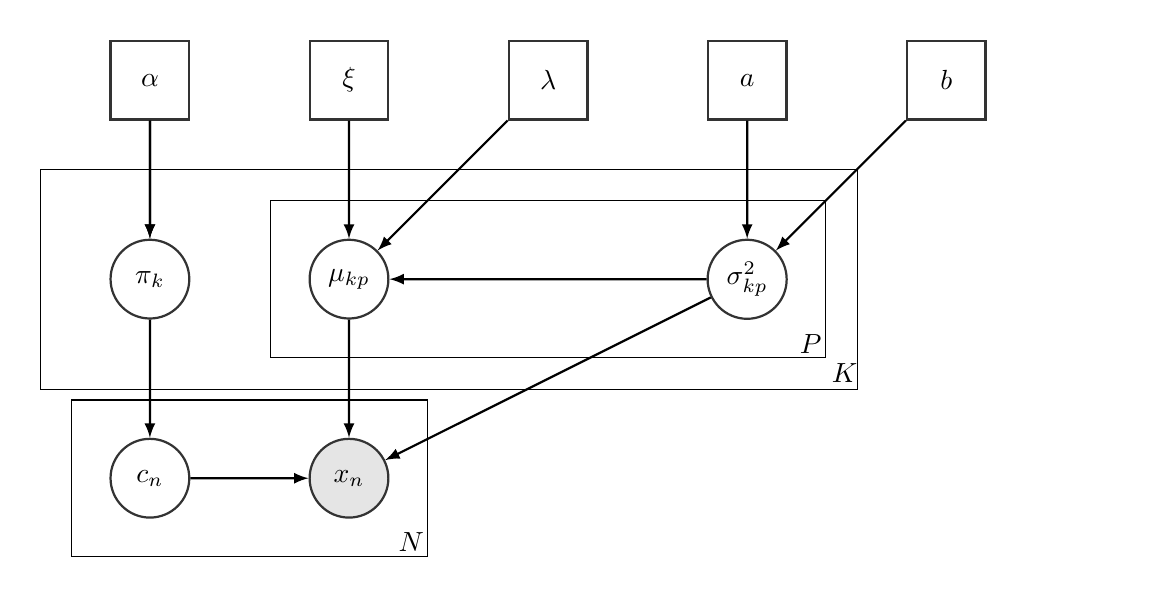
\begin{tikzpicture}[background rectangle/.style={fill=white!1}, show background rectangle, scale=.4, auto,>=latex']
		\tikzstyle{main}=[circle, minimum size = 10mm, thick, draw =black!80, node distance = 15mm]
		\tikzstyle{connect}=[-latex, thick]
		\tikzstyle{box}=[rectangle, draw=black!100]
		%\node[main] (k) {$K$ };
		\node[main, rectangle] (kappa) {$\lambda$};
		\node[main, rectangle] (xi) [left =of kappa] {$\xi$ };
		\node[main, rectangle] (alpha) [left =of xi] {$\alpha$ };
		%		\node[main] (k) [above =of alpha] {$K$};
		\node[main, rectangle] (alpha2) [right =of kappa] {$a$ };
		\node[main, rectangle] (beta) [right =of alpha2] {$b$ };
		\node[main] (pi) [below =of alpha] {$\pi_k$ };
		\node[main] (c_i) [below =of pi] {$c_n$};
		\node[main] (mu) [below=of xi] {$\mu_{kp}$};		
		\node[main] (sigma) [below =of alpha2] {$\sigma^2_{kp}$};
		\node[main, fill = black!10] (x_i) [below =of mu] {$x_n$};
		\node[rectangle, inner sep=-0.5mm, fit= (c_i) (x_i),label=below right:$N$, xshift=13mm, yshift=-1mm] {};
		\node[rectangle, inner sep=4.8mm,draw=black!100, fit= (c_i) (x_i)] {};
		\node[rectangle, inner sep=-0.8mm, fit= (mu) (pi) (sigma),label=below right:$K$, xshift=43mm, yshift=-5mm] {};
		\node[rectangle, inner sep=8.8mm, draw=black! 100, fit= (mu) (pi) (sigma)] {};
		\node[rectangle, inner sep=-0.5mm, fit= (mu) (sigma),label=below right:$P$, xshift=26mm, yshift=-1mm] {};
		\node[rectangle, inner sep=4.8mm, draw=black! 100, fit= (mu) (sigma)] {};
		\path 
		%		(k) edge [connect, bend right=30] (pi)
		%		(k) edge [connect, bend left=30] (c_i)
		%(k) edge [connect, bend left=30] (mu)
		%(k) edge [connect] (sigma)
		(alpha) edge [connect] (pi)
		(pi) edge [connect] (c_i)
		(alpha) edge [connect] (pi)
		(c_i) edge [connect] (x_i)
		(mu) edge [connect] (x_i)
		(sigma) edge [connect] (x_i)
		(sigma) edge [connect] (mu)
		(xi) edge [connect] (mu)
		(kappa) edge [connect] (mu)
		(alpha2) edge [connect] (sigma)
		(beta) edge [connect] (sigma)
		%(k) edge[connect, bend right=30] (x_i)
		;
	\end{tikzpicture}
	\caption{Directed acyclic graph for the mixture of Gaussians used.}
	\label{fig:simpleMixNormalsDAG}
\end{figure}

\subsection{Integrative clustering}
We are interested in the use of Consensus clustering for integrative methods. We used Multiple Dataset Integration \citep[\textbf{MDI}, ][]{kirk2012bayesian} as an example of a Bayesian integrative clustering method. MDI models dataset specific clusterings, in contrast to, for example, Clusternomics \citep{gabasova2017clusternomics} in which a \emph{global clustering} is inferred.

%We use the implementation made by \citep{mason2016mdi} which produces MCMC samples of the allocation vector and is thus suited to our construction of Consensus clustering.

%Bayesian mixture models have been extended to the multiple dataset context where they are used to perform integrative clustering. This means that as much pertinent information as possible can be included in the joint model. Multiple Dataset Integration \citep[\textbf{MDI}, ][]{kirk2012bayesian} is an example of such a model where dataset specific clusterings are learnt, informed by common information. We use MDI to model the clustering structure of the Yeast datasets in section \ref{sec:yeast}. The modelling of the shared information is described by the prior distribution on item allocation for $L$ datasets
The defining aspect of MDI is the prior on the allocation of the $n^{th}$ item across the $L$ datasets
\begin{align}
	p(c_{n1}, \ldots, c_{nL}) \propto \prod_{l=1}^L \pi_{c_{nl}l}\prod_{l=1}^{L-1}\prod_{m=l+1}^L(1 + \phi_{lm} \mathbb{I}(c_{nl} = c_{nm})) \textrm{ for $n = 1,\ldots,N$.}
	\label{eqn:mdiPrior}
\end{align}
$\phi_{lm}$ is the parameter defined by the similarity of the clusterings for the $l^{th}$ and $m^{th}$ datasets and is also sampled in each iteration. As $\phi_{lm}$ increases more mass is placed on the common partition for these datasets. Conversely, in the limit $\phi_{lm}\to 0$ we have independent mixture models. In other words, MDI allows datasets with similar clustering of the items to inform the clustering in each other more strongly than the clustering for an unrelated dataset. The DAG for this model for three datasets is shown in figure \ref{fig:MDIDAG}.
\begin{sidewaysfigure}
	\centering
	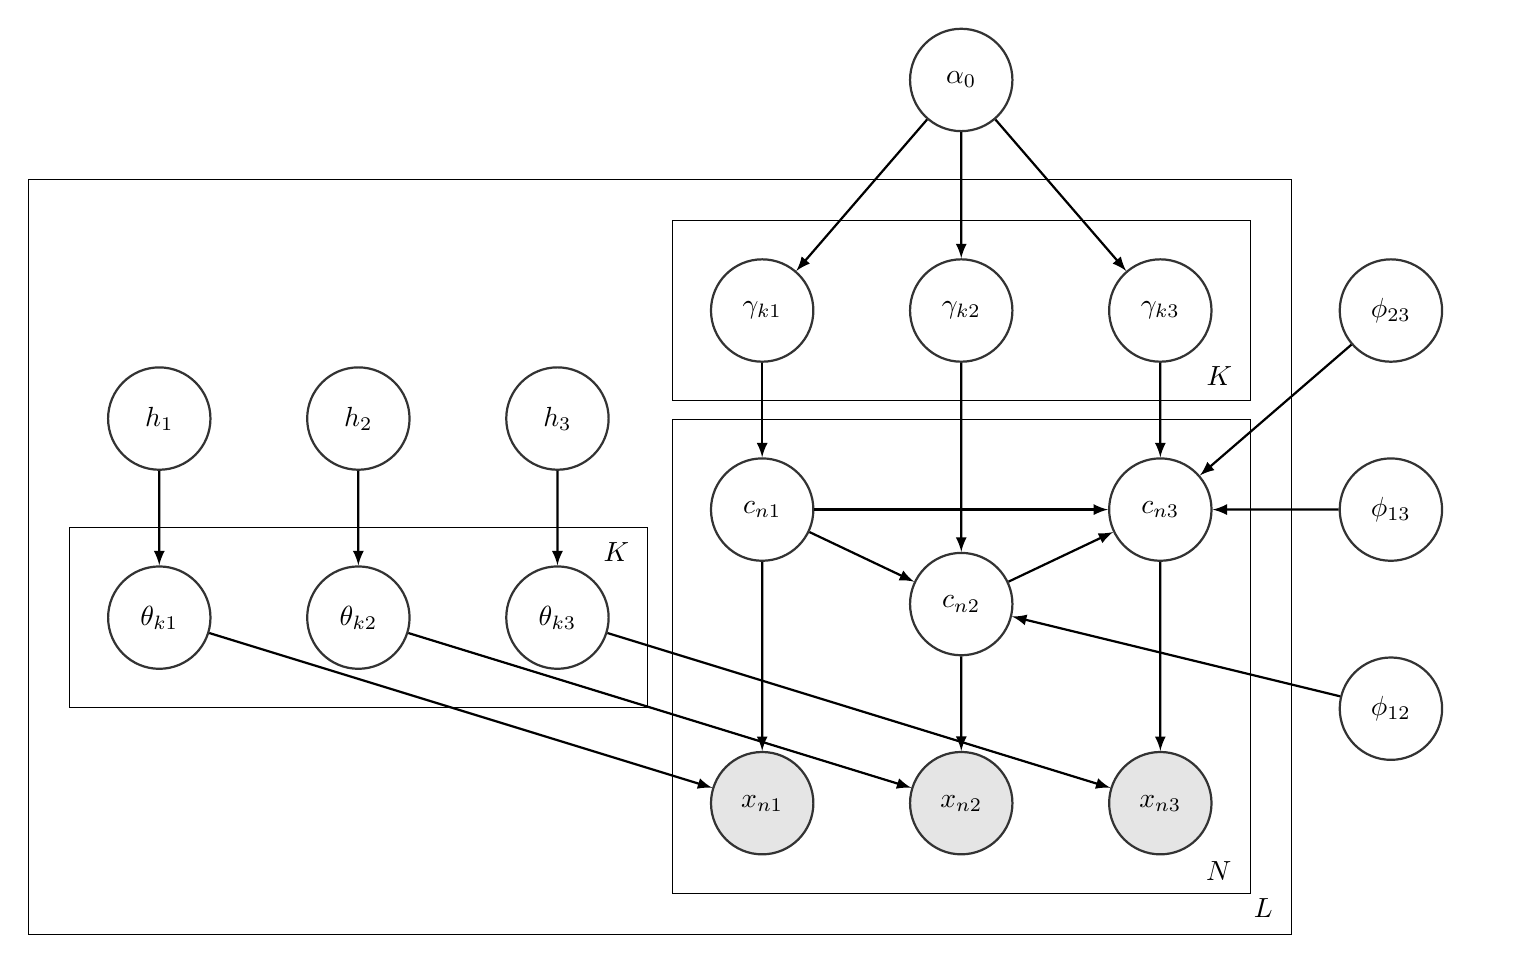
\begin{tikzpicture}[scale=.65, auto,>=latex']
	\tikzstyle{main}=[circle, minimum size = 13mm, thick, draw =black!80, node distance = 12mm]
	\tikzstyle{connect}=[-latex, thick]
	\tikzstyle{box}=[rectangle, draw=black!100]
	
	\node[main] (pi1) {$\gamma_{k1}$ };
	\node[main] (pi2) [right=of pi1] {$\gamma_{k2}$ };
	\node[main] (pi3) [right=of pi2] {$\gamma_{k3}$ };
	
	\node[main] (ci1) [below=of pi1] {$c_{n1}$};
	\node[main, node distance = 24mm] (ci2) [below=of pi2] {$c_{n2}$};
	\node[main] (ci3) [below=of pi3] {$c_{n3}$};
	
	\node[main, node distance = 16mm] (a) [above=of pi2] {$\alpha_0$ };
	
	\node[main, fill = black!10] (xi2) [below=of ci2] {$x_{n2}$}; 
	\node[main, fill = black!10] (xi1) [left=of xi2] {$x_{n1}$};
	\node[main, fill = black!10] (xi3) [right=of xi2] {$x_{n3}$};
	
	\node[main]  at (-4, -6) (theta3) {$\theta_{k3}$}; 
	\node[main] (theta2) [left=of theta3] {$\theta_{k2}$};
	\node[main] (theta1) [left=of theta2] {$\theta_{k1}$};
	
	
	\node[main] (h1) [above=of theta1] {$h_1$};
	\node[main] (h2) [above=of theta2] {$h_2$};
	\node[main] (h3) [above=of theta3] {$h_3$};
	
	\node[main, minimum size=1.3cm, node distance = 16mm] (phi13) [right=of ci3] {$\phi_{13}$}; 
	\node[main, minimum size=1.3cm] (phi12) [below=of phi13] {$\phi_{12}$};
	\node[main, minimum size=1.3cm] (phi23) [above=of phi13] {$\phi_{23}$};
	
	\node[rectangle, inner sep=-0.5mm, fit= (ci1) (ci2) (ci3) (xi1) (xi2) (xi3),label=below right:$N$, xshift=5mm, yshift=0mm] {};
	\node[rectangle, inner sep=4.8mm,draw=black!100, fit= (ci1) (ci2) (ci3) (xi1) (xi2) (xi3)] {};
	
	% \node[rectangle, inner sep=-0.8mm, fit= (theta1) (theta2) (theta3) (pi1) (pi2) (pi3) ,label=above right:$K$, xshift=63mm] {};
	% \node[rectangle, inner sep=4.8mm, draw=black! 100, fit= (theta1) (theta2) (theta3) (pi1) (pi2) (pi3)] {};
	
	\node[rectangle, inner sep=-0.8mm, fit= (theta1) (theta2) (theta3) ,label=above right:$K$, xshift=24mm] {};
	\node[rectangle, inner sep=4.8mm, draw=black! 100, fit= (theta1) (theta2) (theta3)] {};
	
	\node[rectangle, inner sep=-0.8mm, fit=  (pi1) (pi2) (pi3) ,label=below right:$K$, xshift=24mm] {};
	\node[rectangle, inner sep=4.8mm, draw=black! 100, fit= (pi1) (pi2) (pi3)] {};
	
	\node[rectangle, inner sep=-0.8mm, fit= (ci1) (ci2) (ci3) (xi1) (xi2) (xi3) (theta1) (theta2) (theta3) (pi1) (pi2) (pi3) (h1) (h2) (h3),label=below right:$L$, xshift=37mm, yshift=-5mm] {};
	\node[rectangle, inner sep=10.0mm, draw=black! 100, fit= (ci1) (ci2) (ci3) (xi1) (xi2) (xi3) (theta1) (theta2) (theta3) (pi1) (pi2) (pi3) (h1) (h2) (h3)] {};
	
	\path (pi1) edge [connect] (ci1)
	(pi2) edge [connect] (ci2)
	(pi3) edge [connect] (ci3)
	
	(ci1) edge [connect] (xi1)
	(ci2) edge [connect] (xi2)
	(ci3) edge [connect] (xi3)
	
	(ci1) edge [connect] (ci2)
	(ci1) edge [connect] (ci3)
	(ci2) edge [connect] (ci3)
	
	(theta1) edge [connect] (xi1)
	(theta2) edge [connect] (xi2)
	(theta3) edge [connect] (xi3)
	
	(h1) edge [connect] (theta1)
	(h2) edge [connect] (theta2)
	(h3) edge [connect] (theta3)
	
	(a) edge [connect] (pi1)
	(a) edge [connect] (pi2)
	(a) edge [connect] (pi3)
	
	(phi12) edge [connect] (ci2)
	(phi13) edge [connect] (ci3)
	(phi23) edge [connect] (ci3);
	
\end{tikzpicture}
	\caption{Directed acyclic graph for the Multiple Dataset Integration model for $L=3$ datasets. $h_l$ is the choice of hyperpriors for the $l^{th}$ dataset.}
	\label{fig:MDIDAG}
\end{sidewaysfigure}

\section{Consensus clustering}
Consensus clustering is an ensemble approach to cluster analysis. Ensembles are often better able to explore the full parameter space than any individual learner in its composition, thus describing more modes within parameters than the individual learners \citep{ghaemi2011review}. Ensembles also offer reductions in computational runtime because most ensemble methods enable use of a parallel environment to improve computation speed \citep{ghaemi2009survey}. 

Consensus clustering \citep{monti2003consensus} is an ensemble method for cluster analysis, previously implemented using $k$-means clustering as the base learner in the R package \texttt{ConsensusClusterPlus} \citep{wilkerson2010consensusclusterplus}. Consensus clustering has been applied in a variety of biomedical setting such as cancer subtyping \citep{lehmann2011identification, verhaak2010integrated}, identifying subclones in single cell analysis \citep{kiselev2017sc3}, and proteomic characterisation of tumours \citep{xu2020integrative}. Consensus clustering applies $S$ independent runs of the based clustering algorithm to peturbed versions of the dataset and combines the $S$ final partitions in a \emph{Consensus matrix} which is used to infer a final clustering. An outline of this algorithm is described in algorithm \ref{algorithm:CC}. The consensus matrix is a symmetric matrix with the $(i, j)^{th}$ entry being the proportions of model runs for which the $i^{th}$ and $j^{th}$ items are clustered together. For a single partition the \emph{coclustering matrix} represents this information, being a binary matrix with the $(i, j)^{th}$ entry indicating if items $i$ and $j$ are allocated to the same cluster.
%definition CM

\begin{algorithm} \label{algorithm:CC}
	\KwData{\(X=(x_1, \ldots, x_N)\)}
	\KwIn{A resampling scheme \emph{Resample} \\ A clustering algorithm \emph{Cluster} \\ Number of resampling iterations $S$ \\ Set of cluster numbers to try $\mathcal{K}=\{K_1, \ldots, K_{max}\}$}
	\KwOut{A predicted clustering, $\hat{Y}$ \\ The predicted number of clusters present $\hat{K}$}
	%	\KwResult{how to write algorithm with \LaTeX2e }
	\Begin{
		\For{$K \in \mathcal{K}$}{
			\tcc{initialise an empty Consensus Matrix}
			$\mathbf{M}^{(K)} \leftarrow \mathbf{0}_{N \times N}$\;
			\For{$s = 1$ \KwTo $S$}{
				$X^{(s)} \leftarrow Resample(X)$\;
				
				\tcc{Cluster the peturbed dataset, represented in a coclustering matrix}
				$\mathbf{B}^{(s)} \leftarrow Cluster(X^{(s)}, K)$\;
				$\mathbf{M}^{(K)} \leftarrow \mathbf{M}^{(K)} + \mathbf{B}^{(s)}$\;
			}
			$\mathbf{M}^{(K)} \leftarrow \frac{1}{S} \mathbf{M}^{(K)}$\;
		}
		$\hat{K} \leftarrow$ best $K \in \mathcal{K}$ based upon all $\mathbf{M}^{(K)}$\;
		$\hat{Y} \leftarrow$ partition $X$ based upon $\mathbf{M}^{(\hat{K})}$\;
	}
	\caption{Consensus Clustering algorithm}
\end{algorithm}

%\subsubsection{Consensus clustering of Bayesian mixture models}
Ensemble methods are rarely applied Bayesian models despite \cite{monti2003consensus} suggesting this. We believe that Bayesian methods are under exploited in the ensemble framework and propose applying Consensus clustering to Bayesian mixture models. Our implementation of this is described in algorithm \ref{algorithm:CCforBayesianMixtures}.

\begin{algorithm} \label{algorithm:CCforBayesianMixtures}
	\KwData{\(X=(x_1, \ldots, x_N)\)}
	\KwIn{A Bayesian mixture model with membership vector \(c=(c_1, \ldots, c_N)\)\\
		A clustering algorithm that generates samples \emph{Cluster}\\
		The number of chains to run, \(S\)\\
		The number of iterations within each chain, \(R\)
	}
	\KwOut{A predicted clustering, $\hat{Y}$ \\ The consensus matrix $\mathbf{M}$}
	%	\KwResult{how to write algorithm with \LaTeX2e }
	\Begin{
		\tcc{initialise an empty Consensus Matrix}
		$\mathbf{M} \leftarrow \mathbf{0}_{N \times N}$\;
		\For{$s = 1$ \KwTo $S$}{
			\tcc{set the random seed controlling initialisation and MCMC moves}
			$set.seed(s)$\;
			\tcc{initialise a random partition on $X$ drawn from the prior distribution}
			$Y_{(0,s)} \leftarrow Initialise(X)$\;
			\For{$r=1$ \KwTo $R$}{
				\tcc{generate a markov chain for the membership vector}
				$Y_{(r,s)} \leftarrow Cluster(c, r)$\;
			}
			\tcc{create a coclustering matrix from the $R^{th}$ sample}
			$\mathbf{B}^{(s)} \leftarrow Y_{(R,s)}$\;
			$\mathbf{M} \leftarrow \mathbf{M} + \mathbf{B}^{(s)}$\;
		}
		$\mathbf{M} \leftarrow \frac{1}{S} \mathbf{M}$\;
		$\hat{Y} \leftarrow$ partition $X$ based upon $\mathbf{M}$\;
	}
	\caption{Consensus Clustering for Bayesian mixture models}
\end{algorithm}

We show via simulation that ensembles consisting of short chains are sufficient to uncover meaningful structure in a number of scenarios including some within which a Gibbs sampler becomes trapped in individual modes for any reasonable length of runtime. The chains are both short and independent, thus their individual runtime is far shorter than the chains traditionally used for Bayesian inference and may also be run in parallel. This means that consensus clustering of Bayesian mixture models offers significant reductions in runtime without sacrifices in performance. As the ensemble can describe multiple modes, the uncertainty present in the consensus matrix can be more representative of the data than the individual modes captured by any single chain.

We then consider the multiple dataset setting. We apply Consensus clustering to an integrative extension of Bayesian mixture models, Multiple Dataset Integration (MDI). We apply this ensemble to three 'omics datasets for \emph{Saccharomyces cerevisiae} and discover biological meaningful clusters. We then compared this result to performing Bayesian inference of MDI.

%We show on three datasets from the original MDI paper that Consensus clustering performs similarly to Bayesian inference of this model, and then using more modern, larger data that Consensus clustering enables implementation of such models in scenarios where the problem of long runtimes and poor mixing previously discouraged this. 

\subsection{Stopping} \label{sec:stopping}
As our ensemble sidesteps the traditional problem of convergence within each chain, we need an alternative stopping criteria for growing the ensemble in chain depth, $R$, and number of chains, $S$. We propose a heuristic based upon the Consensus matrix to decide if a given value of $R$ and $S$ are sufficient. We suspect that increasing $S$ and $R$ might continuously improve the performance of the ensemble, but we believe that these improvements will become smaller and smaller for greater values, approaching some asymptote for each of $S$ and $R$. Following this logic if the Consensus matrices for three ensembles define by the parameters $(aR, S), (R, bS)$ and $(R, S)$ are not visibly different for some reasonable values of $a, b, S$ and $R$ than increasing ensemble size or depth will see at most marginal improvement in performance. We suggest bounds of $a, b \in (0, 0.5]$ and $R \geq 100, S \geq 50$, but make the general observation that large $S$ and $R$ are always good and that the closer $a$ and $b$ are to 0 the more strict the stopping criteria become.

\section{Simulations} \label{sec:simulations}
We defined a number of scenarios to test certain concepts of the method and to explore behaviour due to specific characteristics of real data. The parameters associated with each scenario in table \ref{table:scenarioTable} were used to generate individual simulations using algorithm \ref{algorithm:simulationGeneration}.
\begin{table}[ht]
	\centering
	% To place a caption above a table
%	\caption{Caption above table.}
	\begin{tabular}{|l|ccccccc|}
	\hline
	\textbf{Scenario} & $N$ & $P_s$ & $P_n$ & $K$ & $\Delta\mu$ & $\sigma^2$ & $\pi$\\
	\hline 
	2D & 100 & 2 & 0 & 5 & 3.0 & 1 &  $(\frac{1}{5} , \frac{1}{5}, \frac{1}{5}, \frac{1}{5}, \frac{1}{5})$ \\
	%		\hline
	No structure & 100 & 0 & 2 & 1 & 0.0 & 1 & 1 \\
	%		\hline
	Base Case & 200 & 20 & 0 & 5 & 1.0 & 1 &  $(\frac{1}{5} , \frac{1}{5}, \frac{1}{5}, \frac{1}{5}, \frac{1}{5})$\\
	%		\hline
	Large standard deviation & 200 & 20 & 0 & 5 & 1.0 & 9 & $(\frac{1}{5} , \frac{1}{5}, \frac{1}{5}, \frac{1}{5}, \frac{1}{5})$ \\
	%		\hline
	Large standard deviation & 200 & 20 & 0 & 5 & 1.0 & 25 &  $(\frac{1}{5} , \frac{1}{5}, \frac{1}{5}, \frac{1}{5}, \frac{1}{5})$\\
	%		\hline
	Irrelevant features & 200 & 20 & 10 & 5 & 1.0 & 1 &  $(\frac{1}{5} , \frac{1}{5}, \frac{1}{5}, \frac{1}{5}, \frac{1}{5})$\\
	%		\hline
	Irrelevant features & 200 & 20 & 20 & 5 & 1.0 & 1 &  $(\frac{1}{5} , \frac{1}{5}, \frac{1}{5}, \frac{1}{5}, \frac{1}{5})$\\
	%		\hline
	Irrelevant features & 200 & 20 & 100 & 5 & 1.0 & 1 &  $(\frac{1}{5} , \frac{1}{5}, \frac{1}{5}, \frac{1}{5}, \frac{1}{5})$\\
	%		\hline
	Varying proportions & 200 & 20 & 0 & 5 & 1.0 & 1 & $(\frac{1}{2} , \frac{1}{4}, \frac{1}{8}, \frac{1}{16}, \frac{1}{16})$ \\
	Varying proportions & 200 & 20 & 0 & 5 & 0.4 & 1 &  $(\frac{1}{2} , \frac{1}{4}, \frac{1}{8}, \frac{1}{16}, \frac{1}{16})$ \\ %(0.5, 0.25, 0.125, 0.0675, 0.0675)\\
	%		\hline
	Small $N$, large $P$ & 50 & 500 & 0 & 5 & 1.0 & 1 &  $(\frac{1}{5} , \frac{1}{5}, \frac{1}{5}, \frac{1}{5}, \frac{1}{5})$\\
	%		\hline
	Small $N$, large $P$ & 50 & 500 & 0 & 5 & 0.2 & 1 &  $(\frac{1}{5} , \frac{1}{5}, \frac{1}{5}, \frac{1}{5}, \frac{1}{5})$
	\\
	\hline
	\end{tabular}
	\caption{Parameters defining the simulation scenarios as used in generating data and labels.}
	\label{table:scenarioTable}
\end{table}%
\begin{algorithm} \label{algorithm:simulationGeneration}
	\TitleOfAlgo{Simulation generation}
	%	\KwData{\(X=(x_1, \ldots, x_N)\)}
	\KwIn{
		%		A random seed $s$\\
		Distance between means \(\Delta_{\mu}\)\\
		A common standard deviation \(\sigma^2\)\\
		A number of clusters \(K\)\\
		The number of items to generate in total \(N\)\\
		The number of features to generate in total \(P\)\\
		An indicator vector of feature relevance \(\phi = (\phi_1, \ldots, \phi_P)\)\\
		The expected proportion of items in each cluster \(\pi=(\pi_1, \ldots, \pi_K)\)\\
		A method for sampling \(x\) times from the array \(y\), with weights \(\pi\): \emph{Sample}\((y, x, \pi)\)\\
		A method for permuting a vector \(x\): \emph{Permute}\((x)\)\\
		A method for generating a value from a univariate Gaussian distribution with mean \(\mu\) and standard deviation \(\sigma^2\): \emph{Gaussian}\((\mu, \sigma^2)\)\\
	}
	\KwOut{A dataset, $X$ \\ The generating cluster labels $c=(c_1, \ldots, c_N)$}
	%	\KwResult{how to write algorithm with \LaTeX2e }
	\Begin{
		%		\tcc{Set the random seed defining the sampling and permuting}
		%		$set.seed(s)$\;
		\tcc{initialise the empty data matrix}
		$X \leftarrow 0_{N \times P}$\;
		\tcc{create a matrix of \(K\) means}
		$\mu \leftarrow (\Delta_{\mu}, \ldots, K\Delta_{\mu})$\;
		\tcc{generate the allocation vector}
		\(c \leftarrow\) \emph{Sample}\((1:K, N, \pi)\)\;
		
		$\mathbf{M} \leftarrow \mathbf{0}_{N \times N}$\;
		\For{$p = 1$ \KwTo $P$}{
			\tcc{Test if the feature is relevant, if relevant generate data from a mixture of univariate Gaussians, otherwise draw all items from the same distribution}
			\If{$\phi_p = 1$}{
				
				%				\tcc{Permute the means associated with each cluster within the current feature to create independent features}
				$\nu \leftarrow$ \emph{Permute}$(\mu)$\;
				
				\For{$n = 1$ \KwTo $N$}{
					%					\tcc{Generate data defined by the original label}
					\(X(n, p) \leftarrow\) \emph{Gaussian}\((\nu_{c_n}, \sigma^2)\)
				}
			}
			\If{$\phi_p = 0$}{
				\For{$n = 1$ \KwTo $N$}{
					\(X(n, p) \leftarrow\) \emph{Gaussian}\((0, \sigma^2)\)
				}
			}
		}
		\tcc{Mean centre and scale the data}
		$X \leftarrow Normalise(X)$
	}
	\caption{Data generation for a mixture of Gaussian with independent features. This algorithm is implemented in the \texttt{generateSimulationDataset} function from the \texttt{mdiHelpR} package available at \texttt{www.github.com/stcolema/mdiHelpR}.}
\end{algorithm}

\begin{itemize}
	\item \emph{2D}: a low dimensional scenario within which we expected \texttt{Mclust} to perform well and the long chains to converge and explore the full support of the posterior distribution.
	\item \emph{No structure}: we included this scenario to reassure fears that Consensus clustering has a predilection to finding clusters where none exist \citep{senbabaoglu2014reassessment,senbabaouglu2014critical}.
	\item \emph{Base case}: highly informative datasets within which we expected methods to find the true generating labels quite easily. We included this scenario to benchmark the others that are variations of this setting.
	\item \emph{Large standard deviation}: these two scenarios investigated the degree of distinction required between clusters for the methods to uncover their structure.
	\item \emph{Irrelevant features}: we included these scenarios to investigate how robust the methods are to irrelevant features.
	\item \emph{Varying proportions}: these scenarios investigated how well each method uncovers clusters when the clusters have significantly different membership counts.
	\item \emph{Small $N$, large $P$}: an investigation of behaviour when the number of features is far greater than the number of items.
\end{itemize}

\subsection{Bayesian analysis} \label{sec:simBayesianAnalysis}
For each simulation we ran 10 chains for 1 million iterations, keeping every thousandth sample. We discarded the first 10,000 iterations to account for burn-in bias, leaving 990 samples per chain. To check if the chains were converged we used
\begin{itemize}
	\item the Geweke convergence diagnostic \citep{geweke1991evaluating} to investigate within-chain stationarity, and
	\item the potential scale reduction factor \citep[$\hat{R}$, ][]{gelman1992inference} and the Vats-Knudson extension \citep[\emph{stable $\hat{R}$},][]{vats2018revisiting} to check across-chain convergence.
\end{itemize}
The Geweke convergence diagnostic is a standard Z-score; it compares the sample mean of two sets of samples (in this case buckets of samples from the first half of the samples to the sample mean of the entire second half of samples). It is calculated under the assumption that the two parts of the chain are asymptotically independent and if this assumption holds (i.e. the chain is sampling the same distribution in both samples) than the scores are expected to be standard normally distributed. If a chain's Geweke convergence diagnostic passed a Shapiro-Wilks test for normality \citep{shapiro1965analysis} (based upon a threshold of 0.05), we considered it to have achieved stationarity and included it in the model performance analysis. 

$\hat{R}$ is expected to approach 1.0 if the set of chains are converged. Low $\hat{R}$ is not sufficient in itself to claim chain convergence, but values above 1.1 are clear evidence for a lack of convergence \citep{gelman2013bayesian}. \cite{vats2018revisiting} show that this threshold is significantly too high (1.01 being a better choice) and propose extensions to $\hat{R}$ that enable a more formal rule for a threshold. We use their method as implemented in the R package \texttt{stableGR} \citep{knudson20202stableGR} as the final check of convergence. An example of the $\hat{R}$ series across the 100 simulations for a scenario where chains are well-behaved is shown in figure \ref{fig:simBaseCaseRhat}.

\begin{figure} %[!tpb]
	\centering
	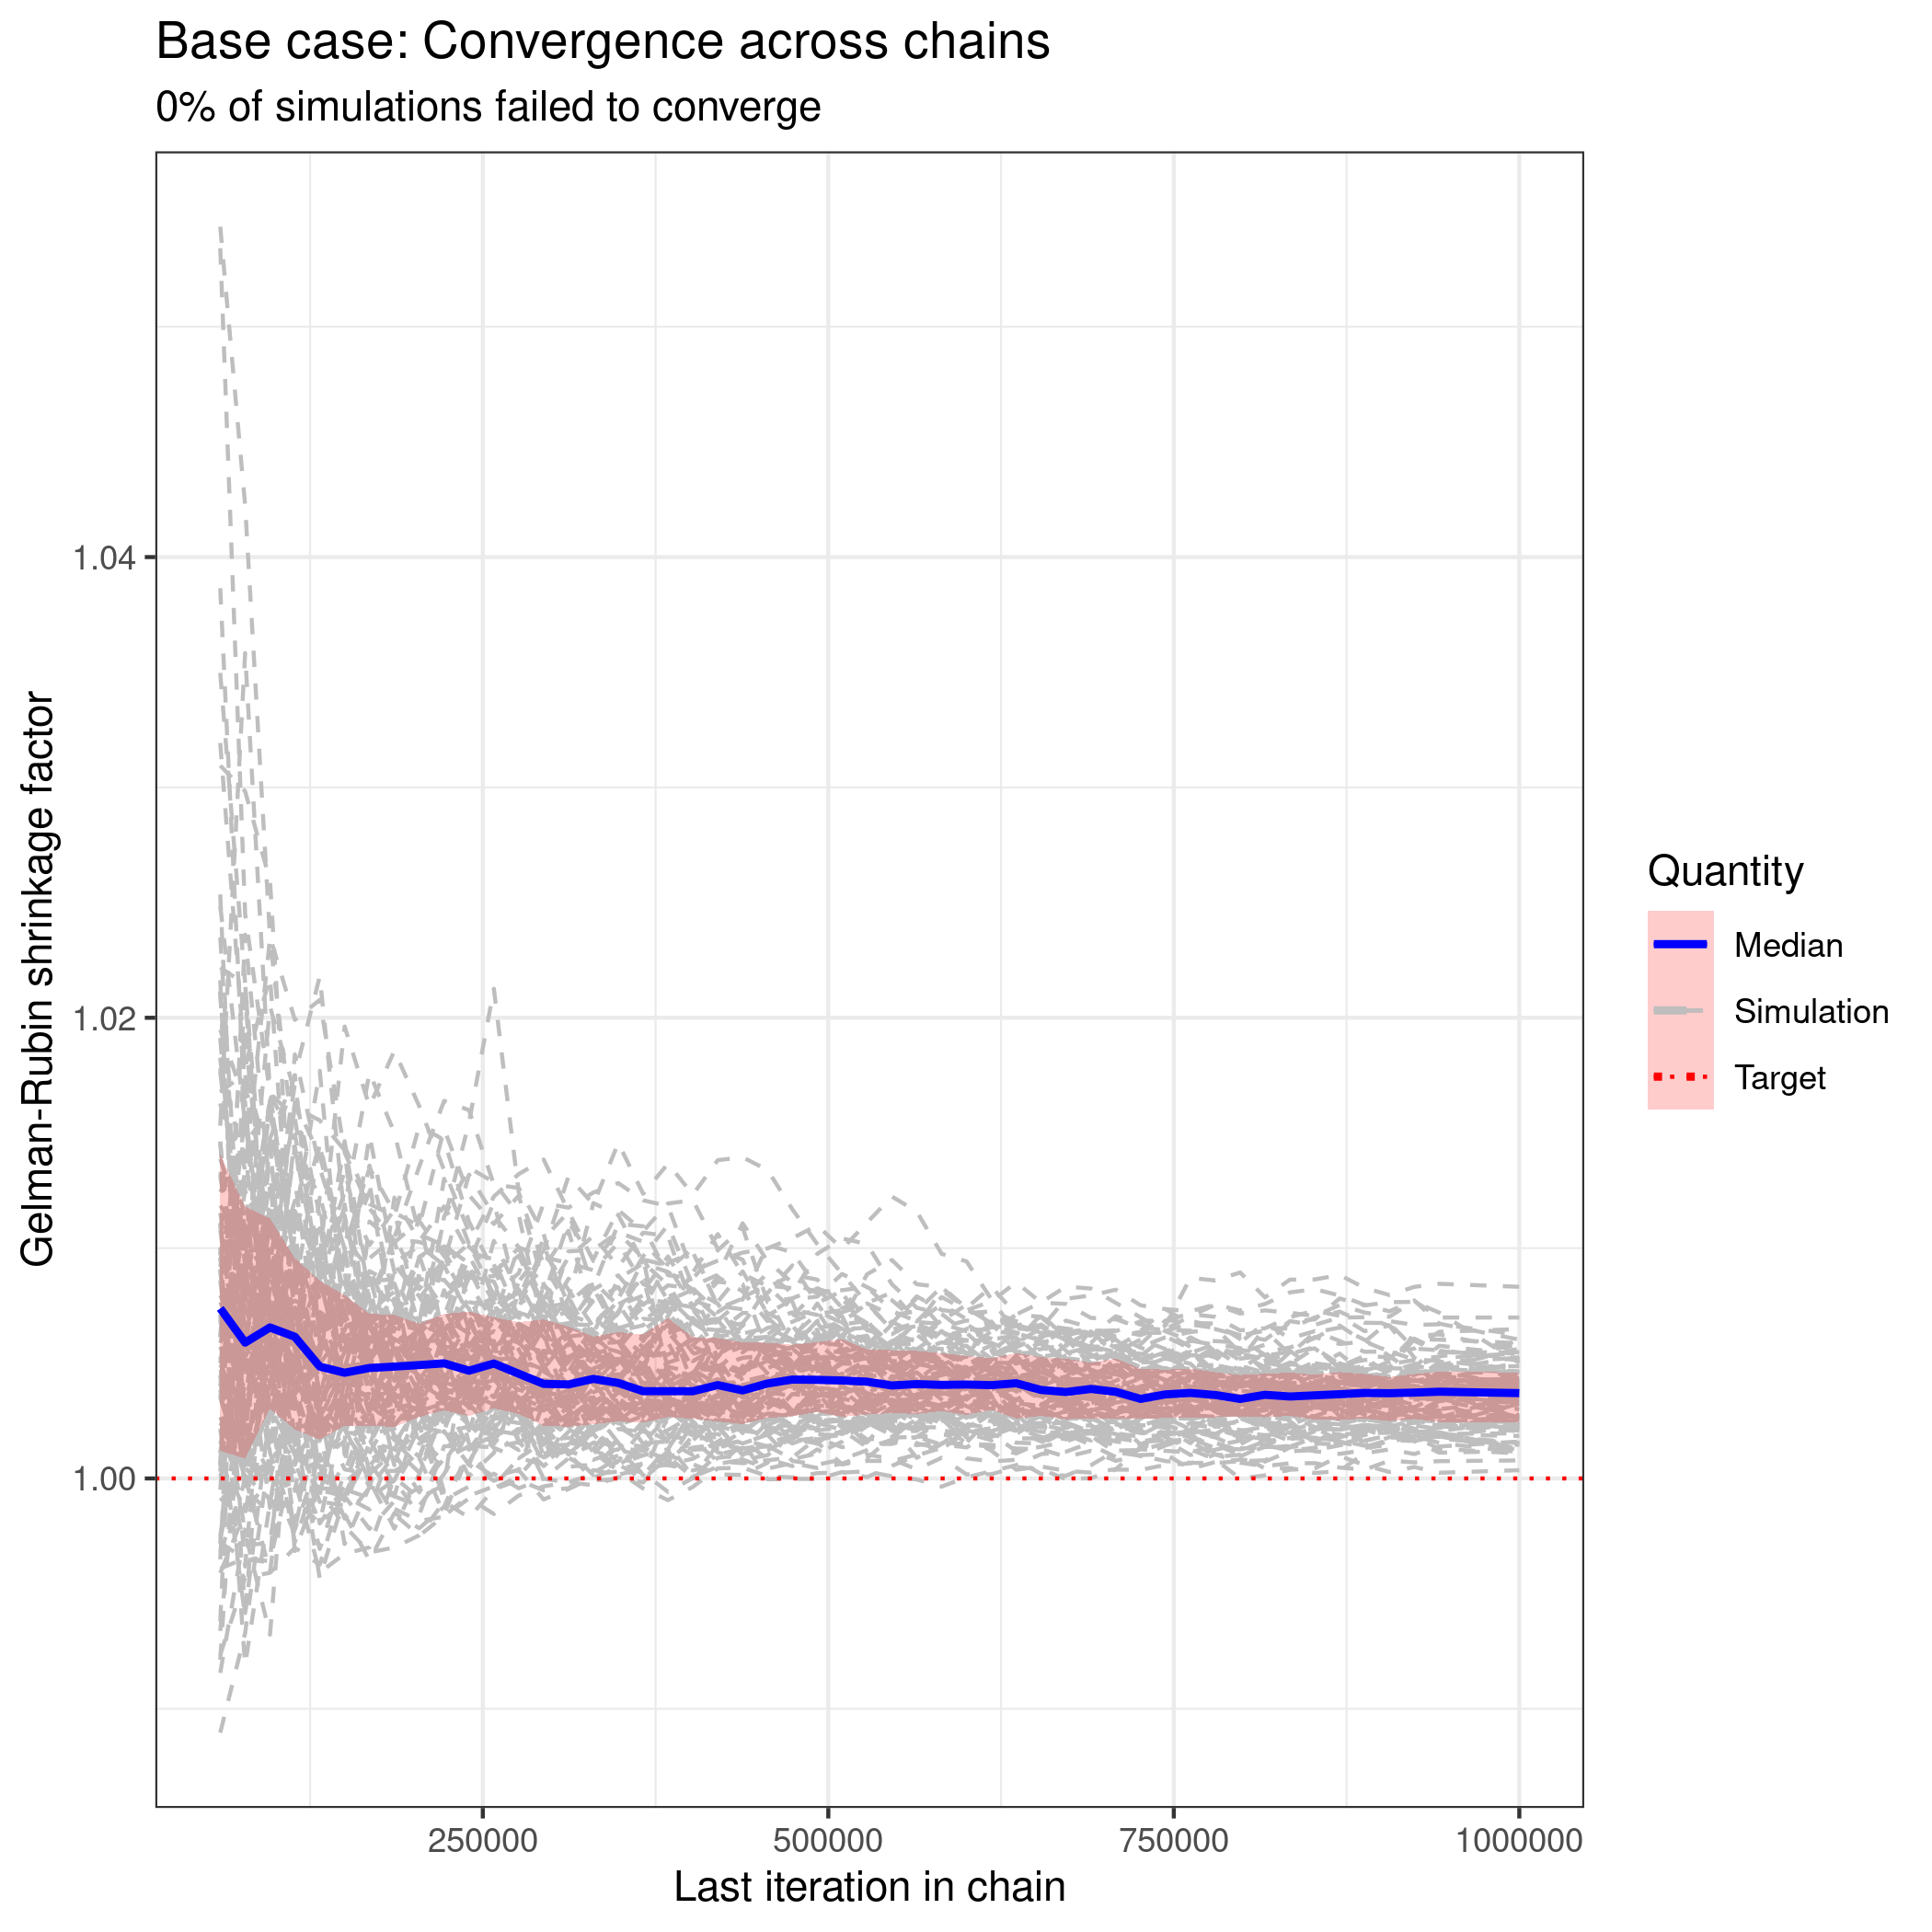
\includegraphics[scale=0.65]{./Images/Simulations/Convergence/base_caseConvergenceAcrossChains.png}
	\caption{The $\hat{R}$ values for each simulation (in dotted grey), the median value and the interquartile range across simulations. One can see that $\hat{R}$ approaches 1.0, being below 1.01 for every simulation by the end of the chains. The ``0\% of simulations failed to converge" is a statement based upon the percentage of simulations which passed the test of stable $\hat{R}$.}
	\label{fig:simBaseCaseRhat}
\end{figure}

We focused upon stationarity of the continuous variables as assesing convergence of the allocation labels is difficult due to label-switching. In our simulations the only recorded continuous variable is the concentration parameter of the Dirichlet distribution for the component weights. 

We pooled the samples from the stationary chains and used these to form a PSM. This and the point estimate clustering found by applying the R function \texttt{maxpear} \citep{fritsch2012mcclust} to this PSM are used in model performance analysis in section \ref{sec:simModelPerformance}. \texttt{maxpear} attempts to find the clustering that maximises the Adjusted Rand Index to the true clustering by using an approximation of the expected clustering under the posterior, $\mathbb{E}(c|X)$, believing that this converges to the true clustering. A sample average clustering is used to approximate the expected clustering. This is estimated from the PSM by maximising
\begin{align}
	\frac{\sum_{i < j}\mathbb{I}(c_i^* = c_j^*) p_{ij} - \sum_{i < j}\mathbb{I}(c_i^* = c_j^*)\sum_{i < j}p_{ij} / {N \choose 2}}{\frac{1}{2}\left[\sum_{i < j}\mathbb{I}(c_i^* = c_j^*) + \sum_{i < j}p_{ij}\right] - \sum_{i < j}\mathbb{I}(c_i^* = c_j^*)\sum_{i < j}p_{ij} / {N \choose 2}}
\end{align}
where $p_{ij}$ is the $(i,j)^{th}$ entry of the PSM \citep{fritsch2009improved}. When the chain has converged this maximises the posterior expected ARI to the true clustering.

There are three possibilities to consider the decision to pool the samples across chains under:
\begin{itemize}
	\item The chains are converged and agree upon the distribution sampled (see figure \ref{fig:simPSMsAgreeExample} for an example).
	\item The chains are not in agreement upon the partition sampled, becoming trapped in different modes. However, a mode does dominate being the mode present in a majority of chains (see figure \ref{fig:simPSMsDisagreeExample} for an example of this behaviour).
	\item The chains are not in agreement and no one mode dominates among chains (see figure \ref{fig:simPSMsPathologicalDisagreeExample} for an example of this behaviour).
\end{itemize}
In the first case pooling has no effect upon the predicted clustering compared to using any one chain. In the second case it feels natural that one would use the mode that dominates. Pooling the samples effectively does this for the predictive performance of the method as the mode with the greatest number of samples across the chains dominates; however, the uncertainty for this mode is increased. In the third case the analysis is non-trivial and further thought, chains and samples would be required. In our simulations this case only arises in the most pathological form in the second \emph{Large $N$, small $P$} scenario, where each chain remains trapped in the initial partition. The clustering inferred from any chain is not meaningful being a random clustering; thus the clustering predicted by pooling the PSMs is no more or less relevant as it too is random. 
%However, the lessening of the certainty around any specific random partition is rewarded under the Frobenius norm.

\begin{figure} %[!tpb]
	\centering
	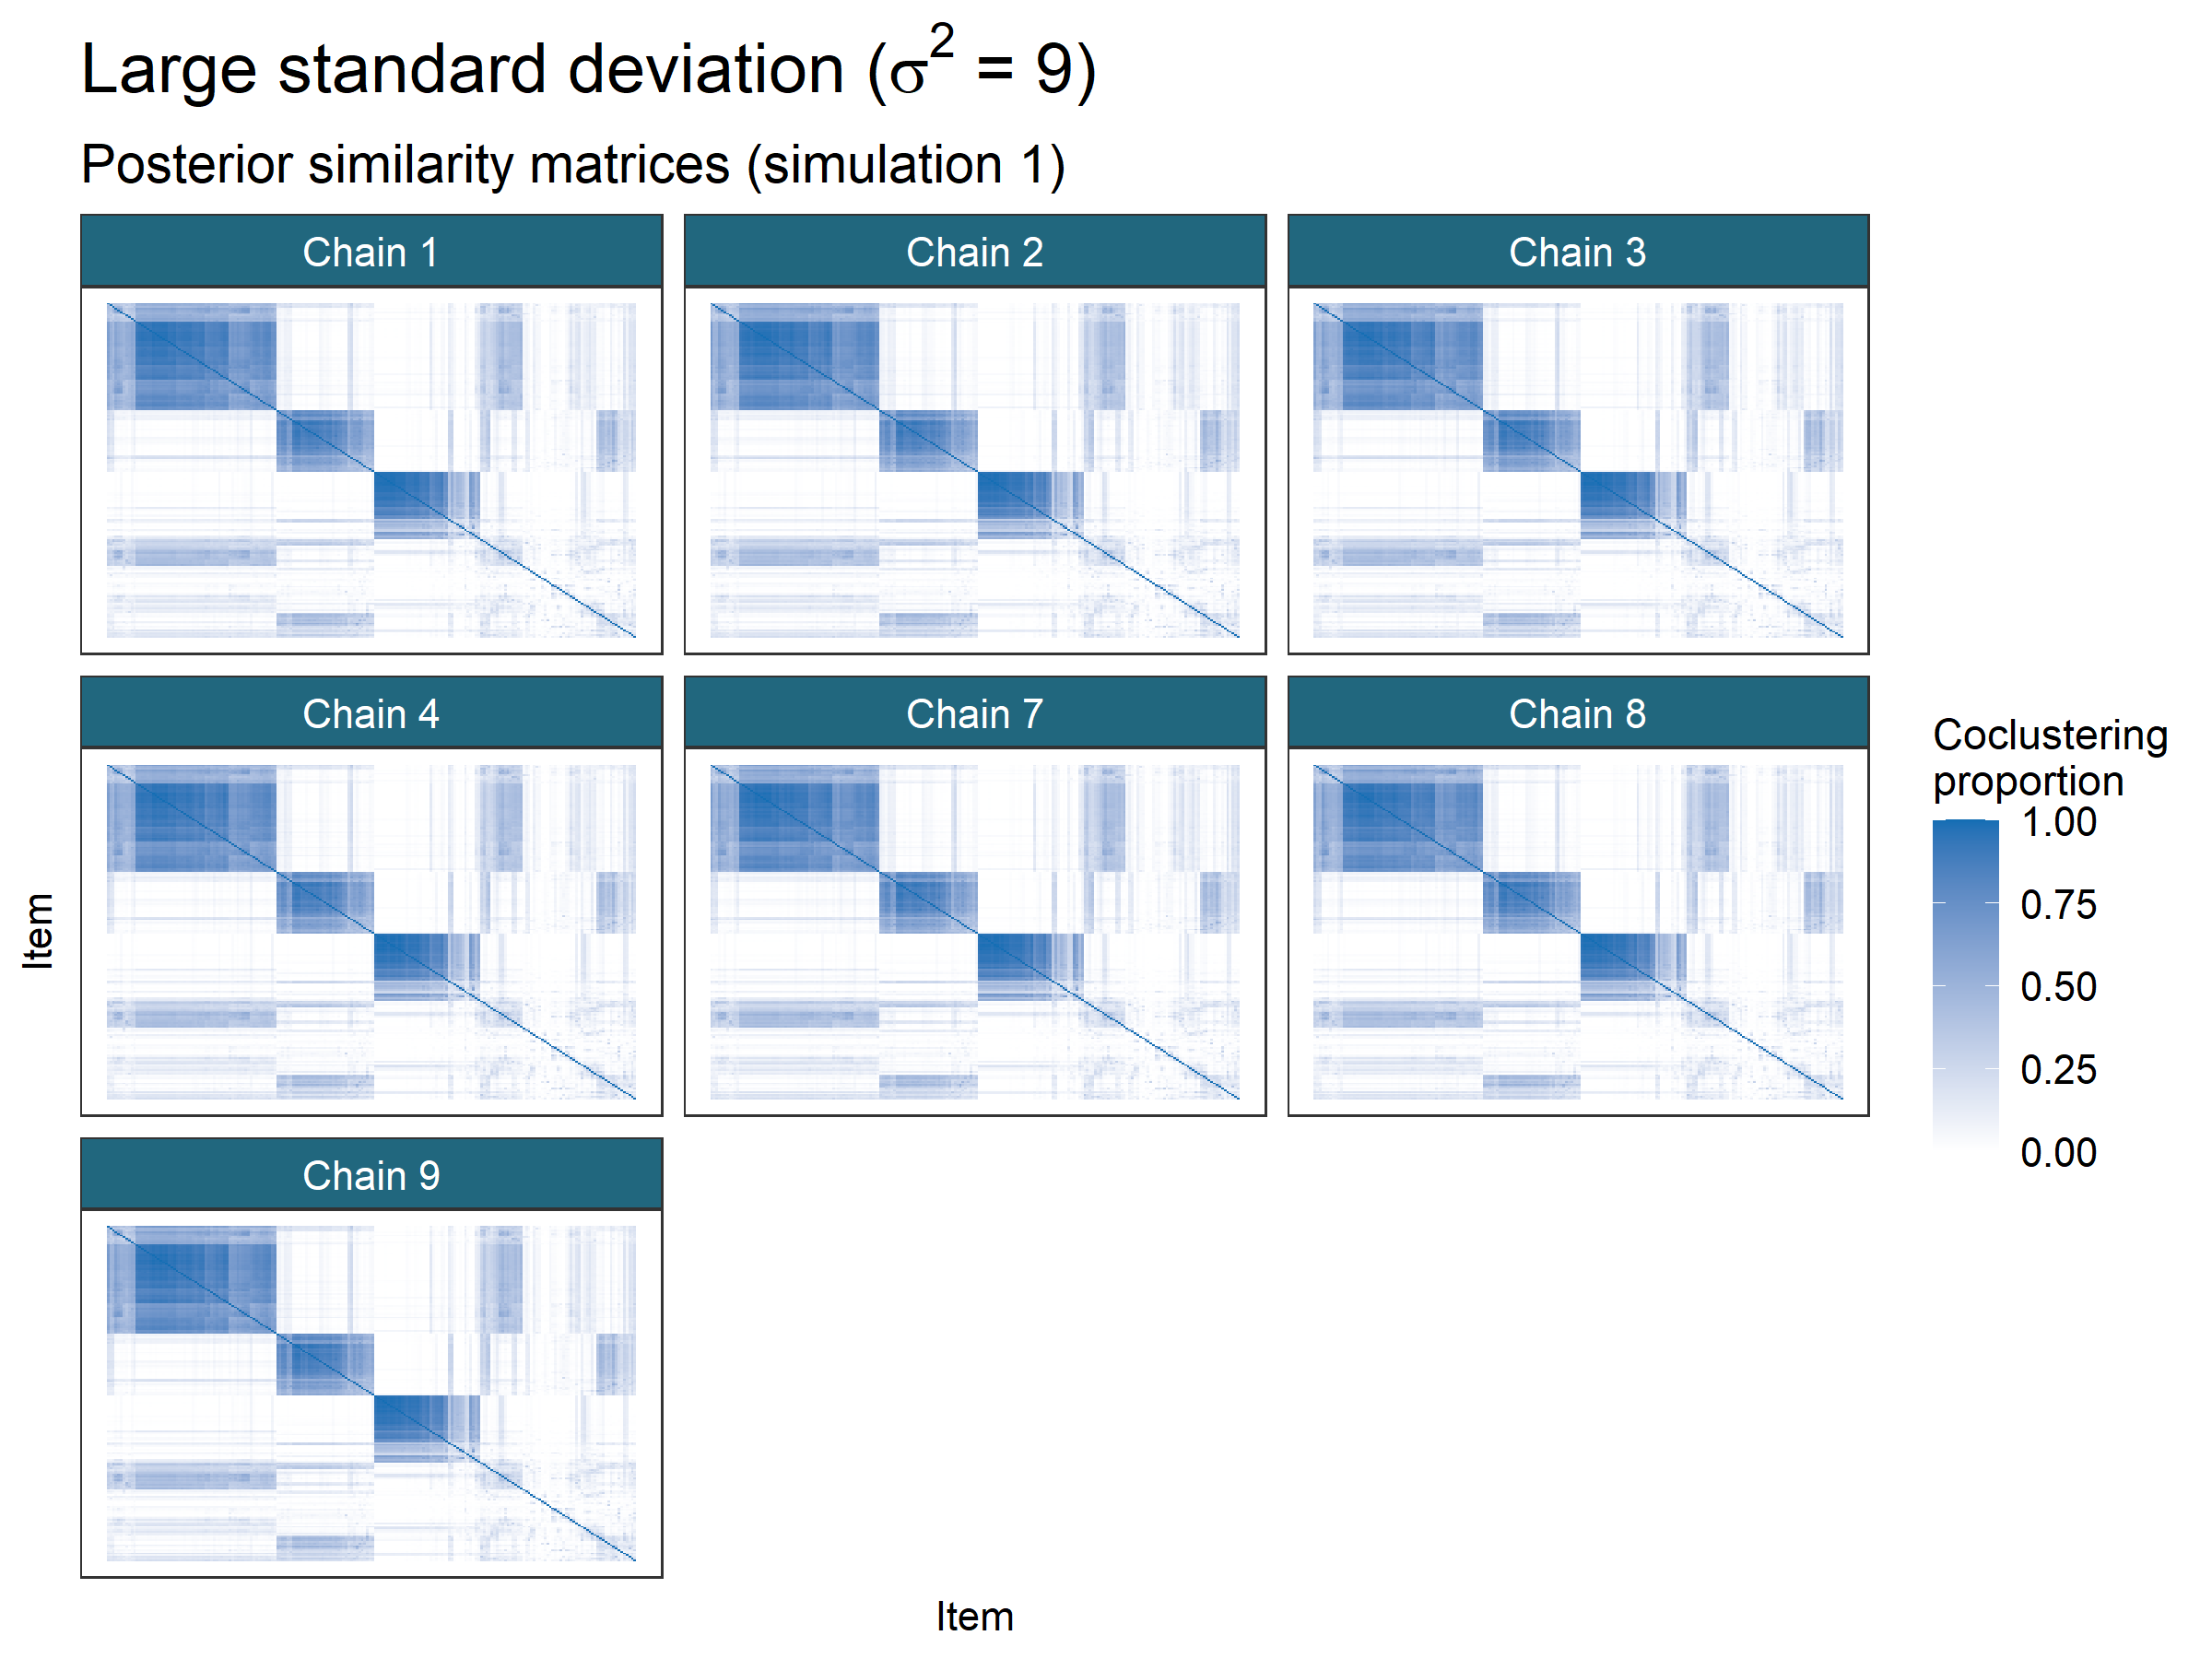
\includegraphics[scale=0.65]{./Images/Simulations/PSMs/large_standard_deviation_3Sim1.png}
	\caption{Posterior similarity matrices for the simulation generated using a random seed set to 1 for the first large standard deviation scenario from table \ref{table:scenarioTable}. This is an example of all stationary chains agreeing in a simulation (and thus pooling of samples is no different to using any choice of chain for the performance analysis). Ordering of rows and columns is defined by hierarchical clustering of the first matrix in the series, in this case that from Chain 1.}
	\label{fig:simPSMsAgreeExample}
\end{figure}

\begin{figure} %[!tpb]
	\centering
	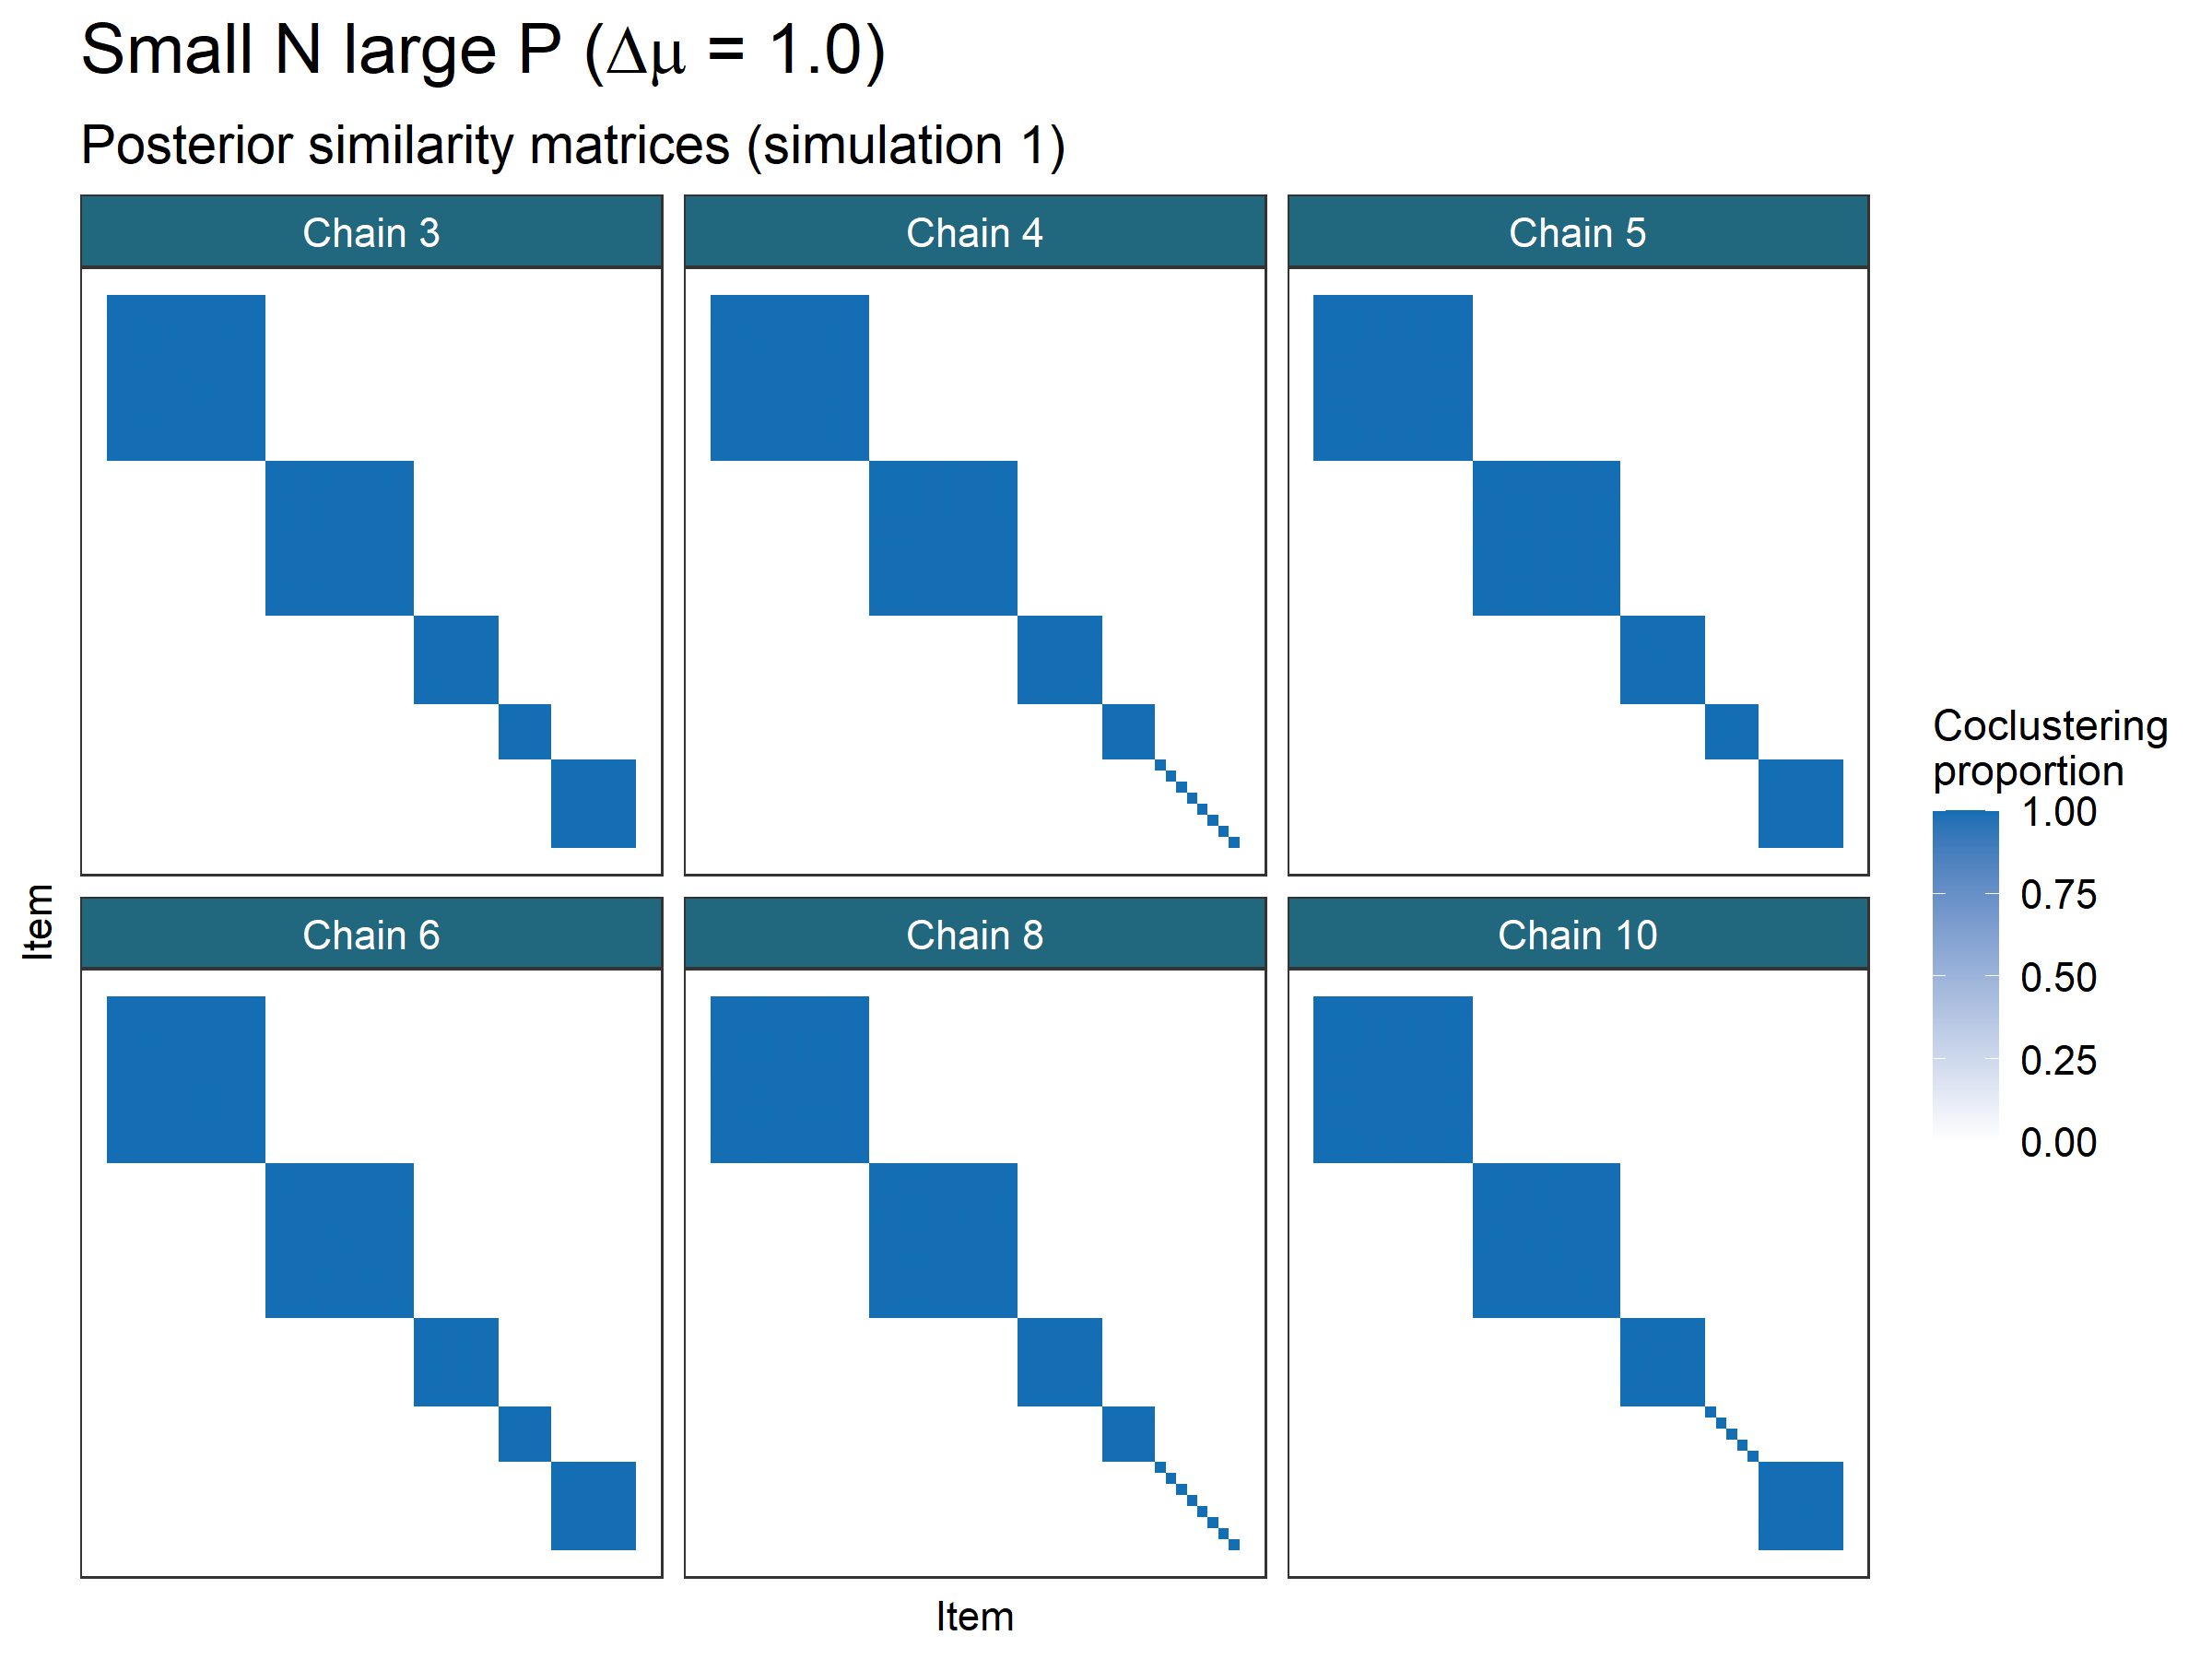
\includegraphics[scale=0.65]{./Images/Simulations/PSMs/small_n_large_p_baseSim1.png}
	\caption{Posterior similarity matrices for the simulation generated using a random seed set to 1 for the first small $N$, large $P$ scenario from table \ref{table:scenarioTable}. This is an example of different chains becoming trapped in different modes, but one mode (which does represent the generating structure well) is dominant, being fully present in 3 of the 6 chains, with the two other modes present having significant overlap. Ordering of rows and columns is defined by hierarchical clustering of the first matrix in the series, in this case that from Chain 1.}
	\label{fig:simPSMsDisagreeExample}
\end{figure}


\begin{figure} %[!tpb]
	\centering
	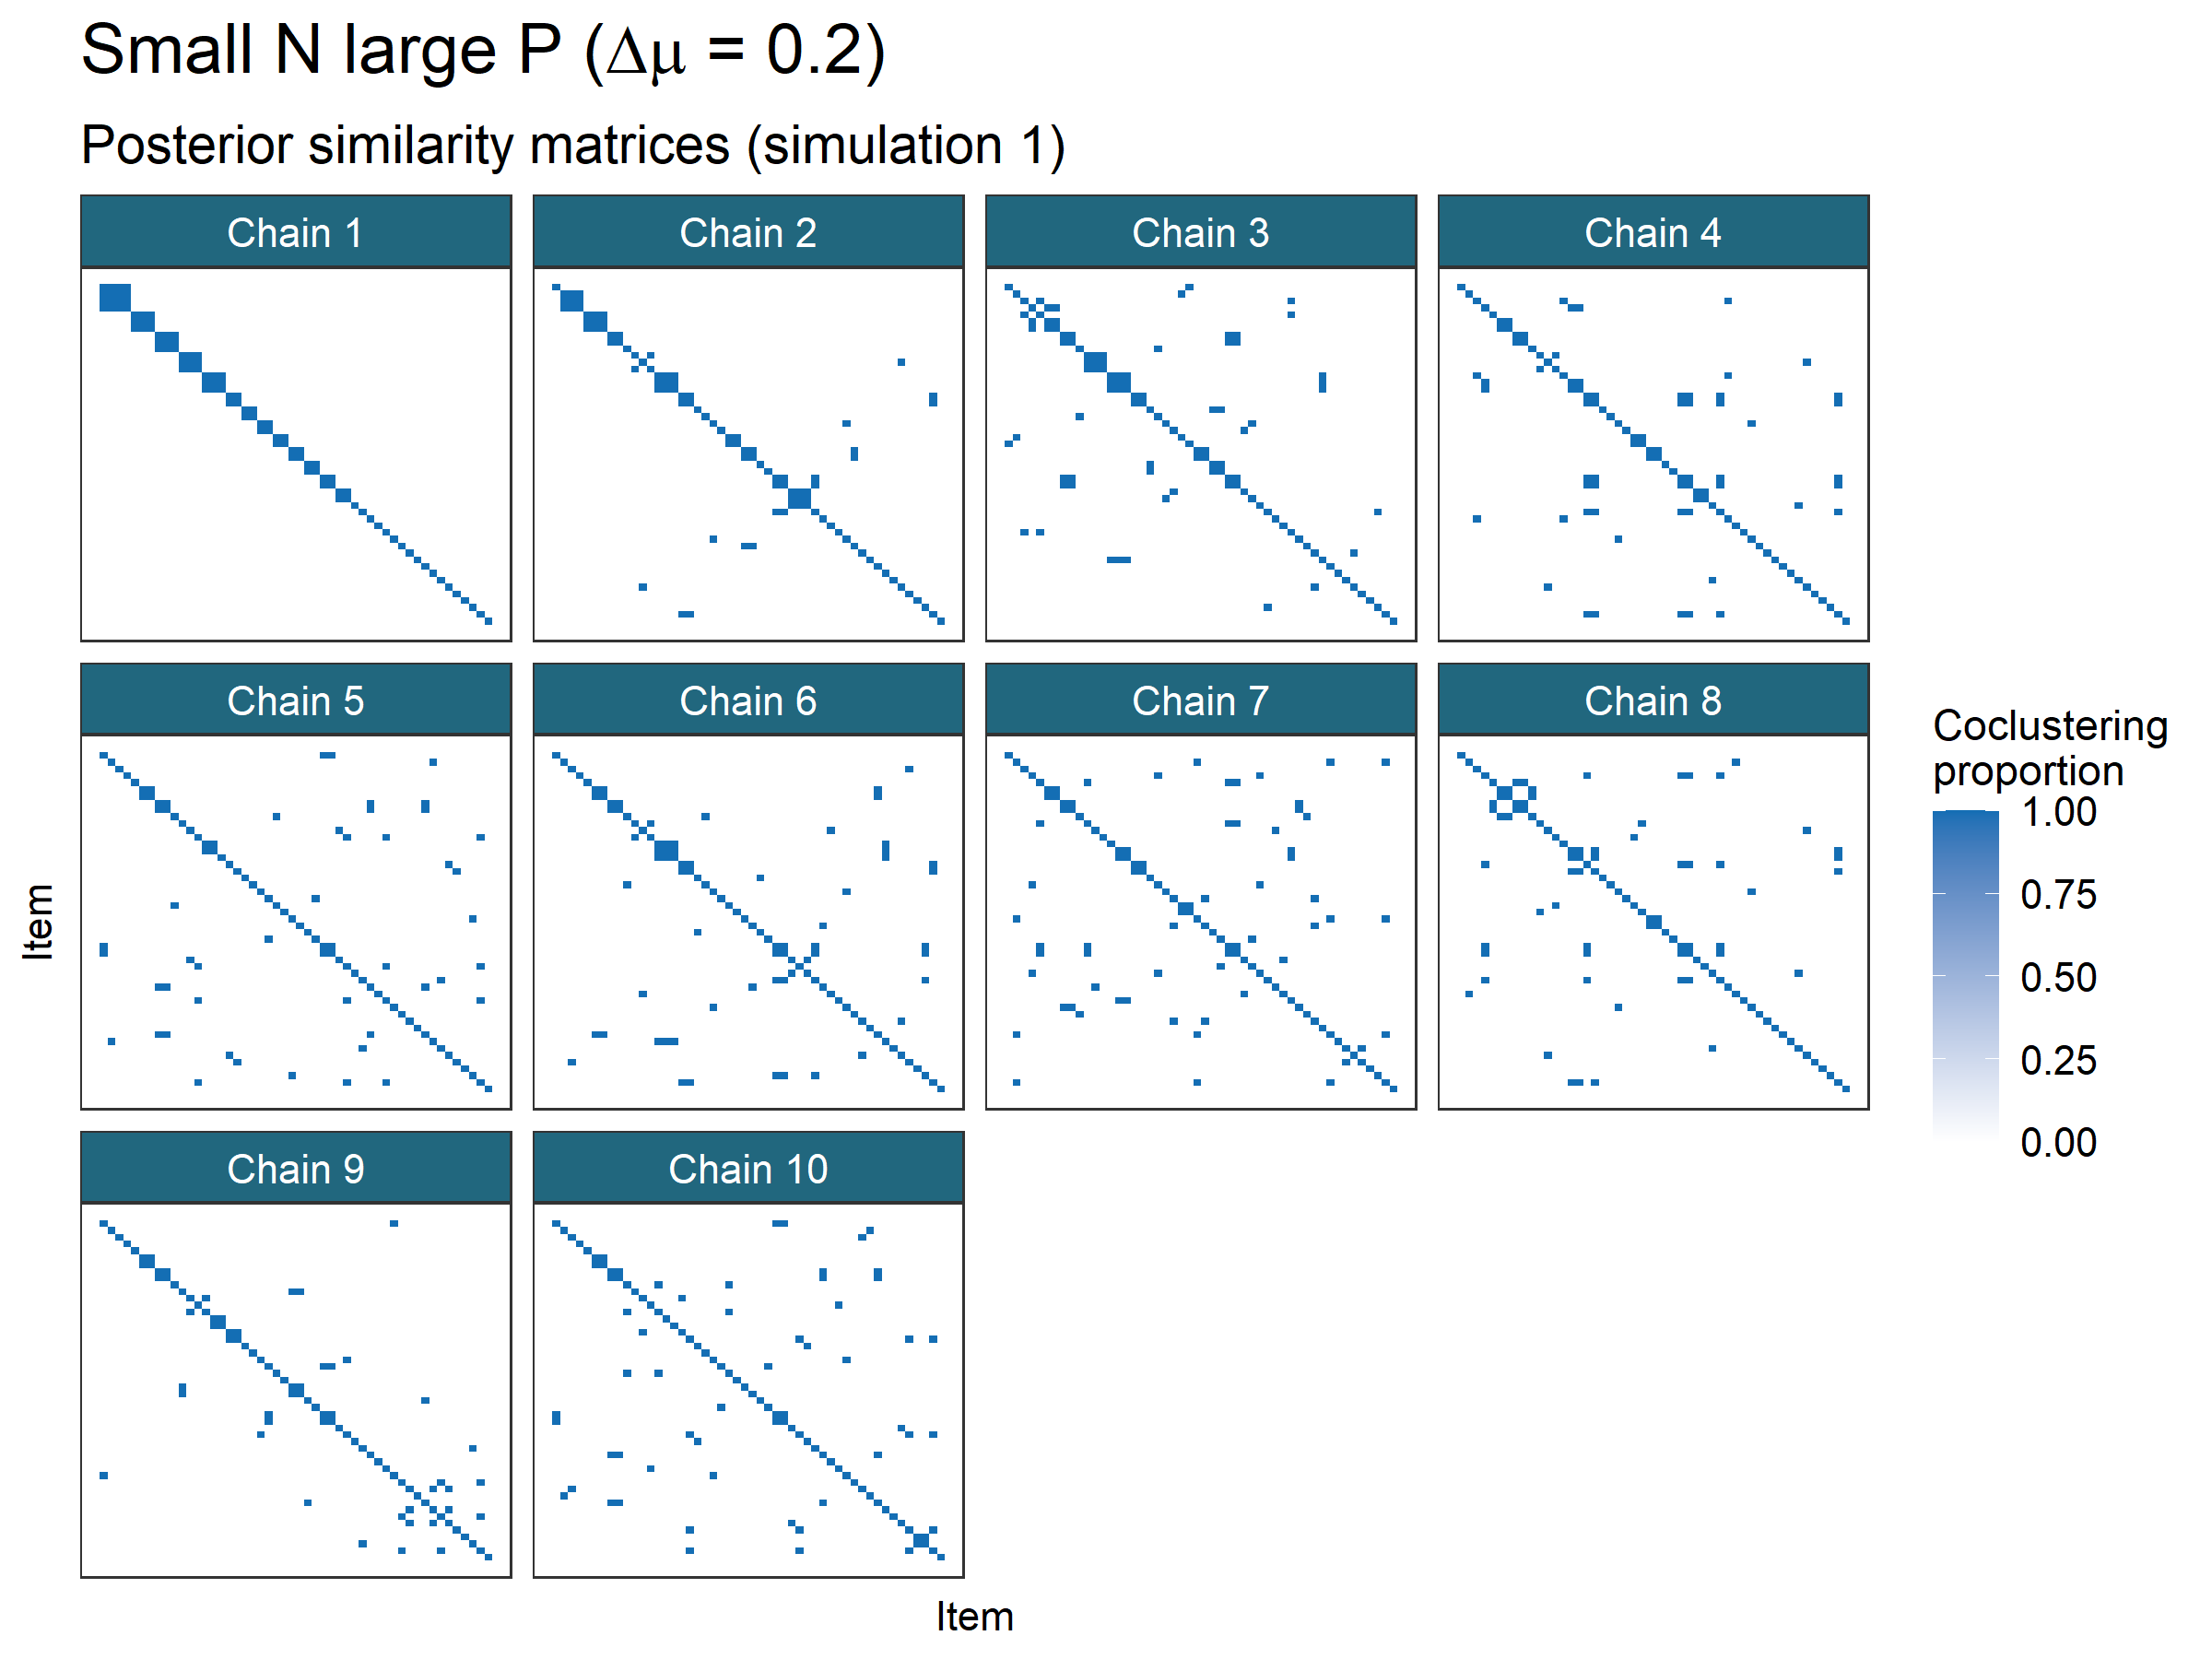
\includegraphics[scale=0.65]{./Images/Simulations/PSMs/small_n_large_p_small_dmSim1.png}
	\caption{Posterior similarity matrices for the simulation generated using a random seed set to 1 for the second small $N$, large $P$ scenario from table \ref{table:scenarioTable}. This is an example of different chains becoming trapped in different modes with no mode being dominant. In this scenario each chain remains trapped in initialisation. Ordering of rows and columns is defined by hierarchical clustering of the first matrix in the series, in this case that from Chain 1.}
	\label{fig:simPSMsPathologicalDisagreeExample}
\end{figure}


\subsection{Consensus clustering analysis} 
We investigated a range of ensembles, using all combinations of chain depth, $R=(1, 10, 100, 1000, 10000)$, and the number of chains, $S=(1, 10, 30, 50, 100)$. This gave a total of 25 different ensembles. A Consensus matrix was constructed from the samples generated by each ensemble by finding the proportion of samples within which any pair of items are coclustered. An example of the Consensus matrices for each ensemble in a given simulation is shown in figure \ref{fig:simCMsIrr100}. We used the \texttt{maxpear} function from the R package \texttt{mcclust} to create a point clustering estimate from the Consensus matrix. In this context where we do not assume that the Consensus matrix of the samples is the Posterior similarity matrix we do not expect that the predicted clustering maximises the posterior expected ARI. Instead \texttt{maxpear} is used as calculating a sample average clustering which we believe is representative of the ensemble.

\begin{figure} %[!tpb]
	\centering
	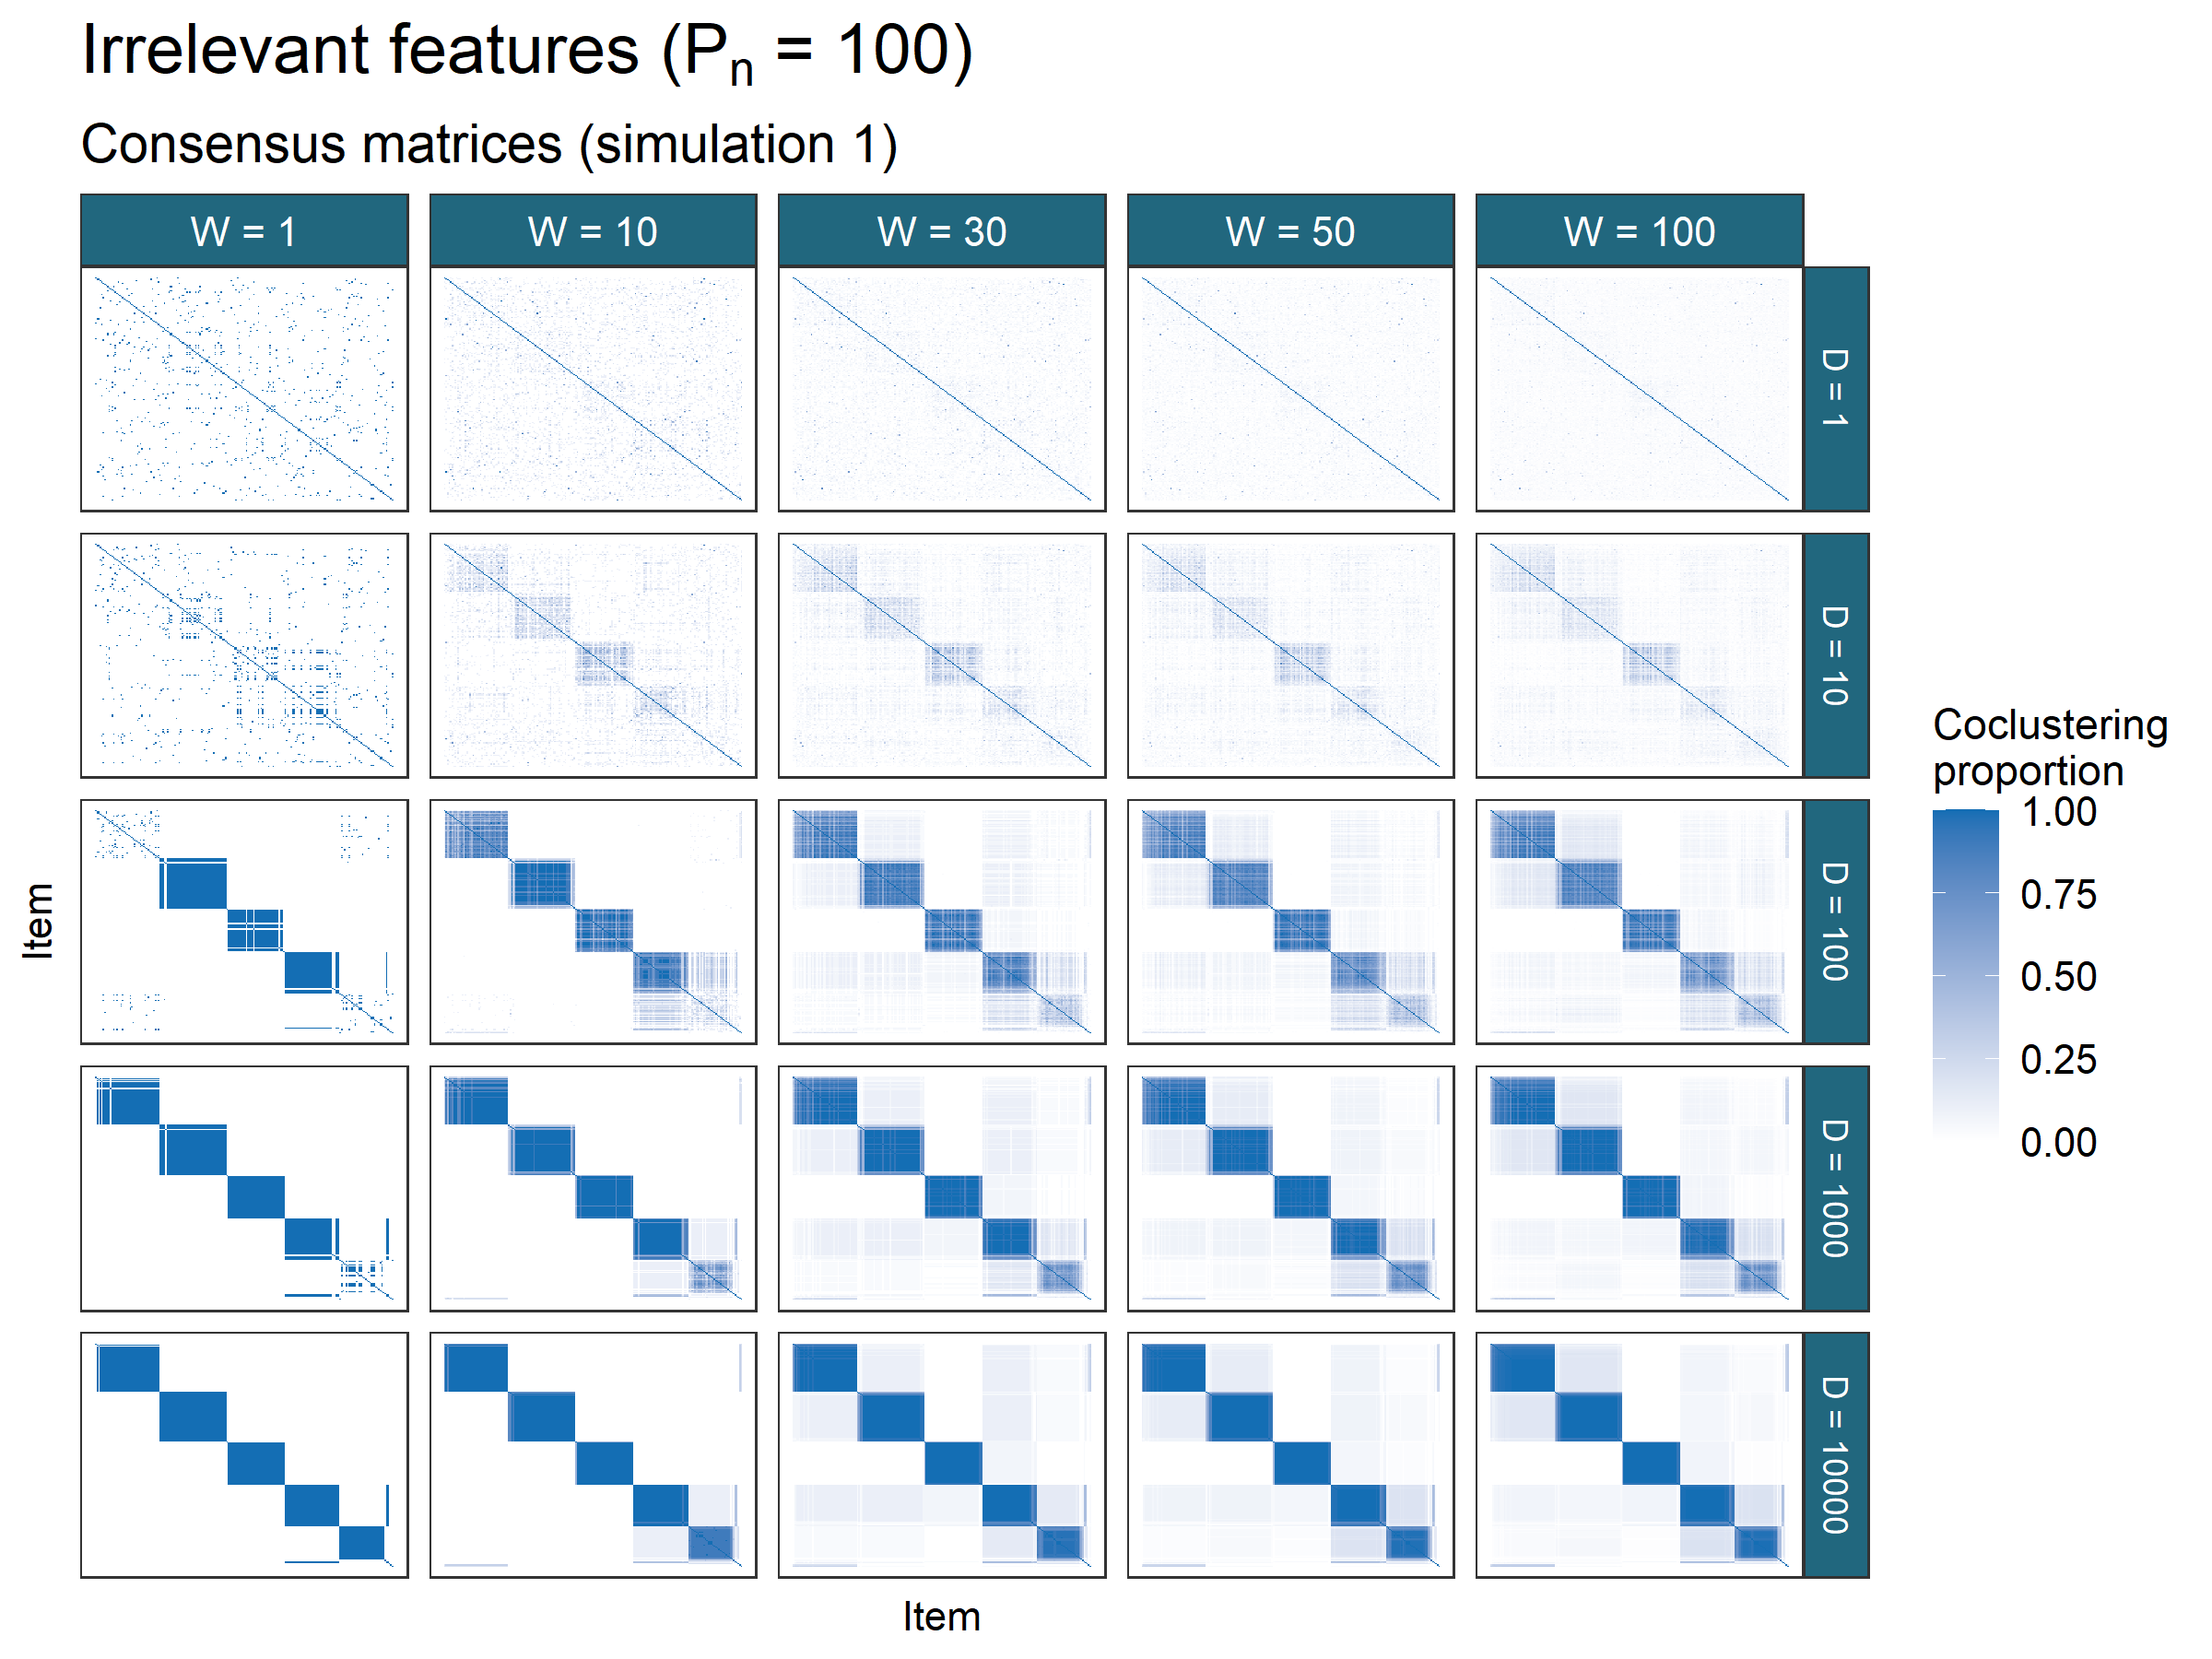
\includegraphics[scale=0.65]{./Images/Simulations/CMs/irrelevant_features_100Sim1.png}
	\caption{Consensus matrices for the simulation generated using a random seed set to 1 for the third irrelevant features scenario from table \ref{table:scenarioTable}. $R$ is the individual chain length and $S$ is the number of chains used. In this example there are several modes present (as seen in the entries with values between 0 and 1) but one mode is clearly dominant (the 5 dark  squares along the diagonal which correspond closely to the generating labels).}
	\label{fig:simCMsIrr100}
\end{figure}


\subsection{\texttt{Mclust}}
We called \texttt{Mclust} using the default settings and a range of inputs for the choice of $K$. We used $K = (2, \ldots, \min(\frac{N}{2}, 50))$ to mirror the choice of $K_{max}=50$ used for the overfitted mixture models (the default in the software we used), with the bound of $\frac{N}{2}$ to avoid fitting 50 clusters in the \emph{Small $N$, large $P$} scenario where $N=50=K_{max}$. In the \emph{No structure} scenarios we extended to range to $K = (1 \ldots, 50)$ to include the correct structure as an option. The model choice was performed using the Bayesian Information Criterion \citep[][as implemented in \texttt{Mclust}]{schwarz1978estimating}.

% An example of each scenario may be seen in figure \ref{fig:genData}

\subsection{Model performance} \label{sec:simModelPerformance}
The different models (Bayesian (pooled), \texttt{Mclust} and the 25 Consensus clustering ensembles) were compared under their ability to predict the generating clustering and their uncertainty about this quantity.

In figure \ref{fig:simPrediction} the ARI between the generating labels and the point estimate clustering from each method is shown. For two partitions $c_1, c_2$, 
\begin{itemize}
	\item $ARI(c_1, c_2) = 1.0$: a perfect match between the two partitions,
	\item $ARI(c_1, c_2) = 0.0$: $c_1$ is no more similar to $c_2$ than is expected for a random partition of the data.
\end{itemize}
In several scenarios \texttt{Mclust} performs the best under this metric (e.g. in the scenarios \emph{2D}, \emph{Small $N$, large $P$ ($\Delta \mu = 0.2$)}). However when the number of irrelevant features is large \texttt{Mclust} performs less well (see \emph{Irrelevant features ($P_n = 20$)} and \emph{($P_n = 100$)}) than the other methods. 
%The decrease in uncertainty due to conditioning on a given number of clusters, $K$, means that when \texttt{Mclust} is correct it is more certain than it might otherwise be. Secondly, 
The initialisation used by \texttt{Mclust} is based upon a hierarchical clustering of the data. We suspect that this contributes to the better performance in the \emph{Small $N$, large $P$ ($\Delta \mu = 0.2$)} case and the poor performance in the presence of large numbers of irrelevant features.

The pooled Bayesian samples act as an upper bound on the Consensus clustering ensembles in these simulations.

For the ensembles there are two parameters changing between each model, the iteration used to provide the clustering in the ensemble, $R$, and the number of chains (and hence samples) used, $S$. In many of the scenarios we find that the benefit of increasing $R$ stabilises by approximately $R = 10$. We believe that in a low-dimensional dataset (such as \emph{2D}), or a highly informative dataset (such as \emph{Base case} or any of the higher dimensional scenarios with no irrelevant features where $\frac{\Delta \mu}{\sigma^2} \geq 1$) the chains quickly find a ``sensible" partition of the data and thus increasing the depth within the chain does not increase the probability that any partition sampled will be closer to the generating partition. For example in figure \ref{fig:simPrediction} in the \emph{Small $N$, large $P$} case, the distribution of the ARI across the ensembles for which $R\geq10$ and $S=1$ is nearly identical; this suggests that the chain is sampling a very similar partition again and again for 9,990 iterations (and possibly beyond based upon the PSMs shown in figure \ref{fig:simPSMsDisagreeExample}) and it is through adding more chains rather than using particularly long chains that we improve the ability to uncover the generating structure. 

We also notice that even if the behaviour has not stabilised for $R$ that the ensemble can uncover meaningful structure. The ARI for the ensembles of short chains can be quite high (as is the case in many of the scenarios). The behaviour of the Consensus matrices also shows that low $R$ is not a disqualifier from meaningful inference even if longer chains would be ideal. Consider the Consensus matrices in figure \ref{fig:simCMsIrr100}, it can be seen that the behaviour has not stabilised before $R=10000$ (and possibly there is still some benefit in increasing $R$ beyond this value), but the structure being uncovered when there is a sufficient number of chains and $R$ is small does correspond to the structure uncovered in the largest and deepest ensemble. We believe that the order in which components merge and items are co-clustered varies depending on initialisation, and thus if the chain is not sufficiently deep that all of the final mergings have occured that a sufficiently large ensemble can still perform meaningful inference of the subpopulation structure. Even though each learner probably has too many clusters for small $R$ the consensus among them will have less. This is why the entries of the Consensus matrix for $R=100$ and $S=100$ in figure \ref{fig:simCMsIrr100} are more pale than in deeper ensembles; very few items correctly (possibly none) cocluster in every partition, it is only in observing the consensus that the global structure of interest emerges. Thus if there is some limit to the length of chains available for an analysis (e.g. computational or temporal constraints) than the inference obtained from the shorter chains can still be meaningful, with the caveat that the point clustering might have more clusters than the same analysis with longer chains would provide. Additional post-hoc merging of some clusters might be necessary in this case.

In contrast, when the dataset is sparse or contains many irrelevant features, we believe that deeper chains are required to reach this steady-state sampling where no single sample is expected to be better than any other (see the \emph{Irrelevant features ($P_n = 100$)} facet of figure \ref{fig:simPrediction}).
%think that in the scenarios with less distinct clusters (i.e. where the number of irrelevant features, $P_n$, is large or $\frac{\Delta \mu}{\sigma^2} \leq 1$), 


In some scenarios no method is successful in uncovering the generating labels. In the \emph{Large standard deviation ($\sigma^2 =25$)} and \emph{Small $N$, large $P$ ($\Delta \mu = 0.2$)} this is due to the lack of signal - the clusters overlap so significantly that it is not possible for any of these methods to uncover much of the generating structure. In the \emph{No structure} case it is different (although \texttt{Mclust} does perform well here). In this case all items are generated from a common distributions. For the Bayesian chains and the ensembles, a clustering of singletons is predicted; each item is allocated a unique label (see figures \ref{fig:simNoStructPSMs} and \ref{fig:simNoStructCMs}). While failing to perform well under the ARI, this is a sensible result. Rather than indicating (as we did with the shared label) that no item is particularly distinct from the others and thus all share a common label, this clustering of singletons states that no item is more similar to any other and thus no two items should cluster together. It is an alternative statement of the same result, i.e. that there is no evidence for subpopulation structure. We consider this evidence that an ensemble of Bayesian mixture models is not as susceptible to predicting labels than an ensemble based upon $K$-means clustering as in \cite{senbabaoglu2014reassessment,senbabaouglu2014critical}.

\begin{figure} %[!tpb]
	\centering
	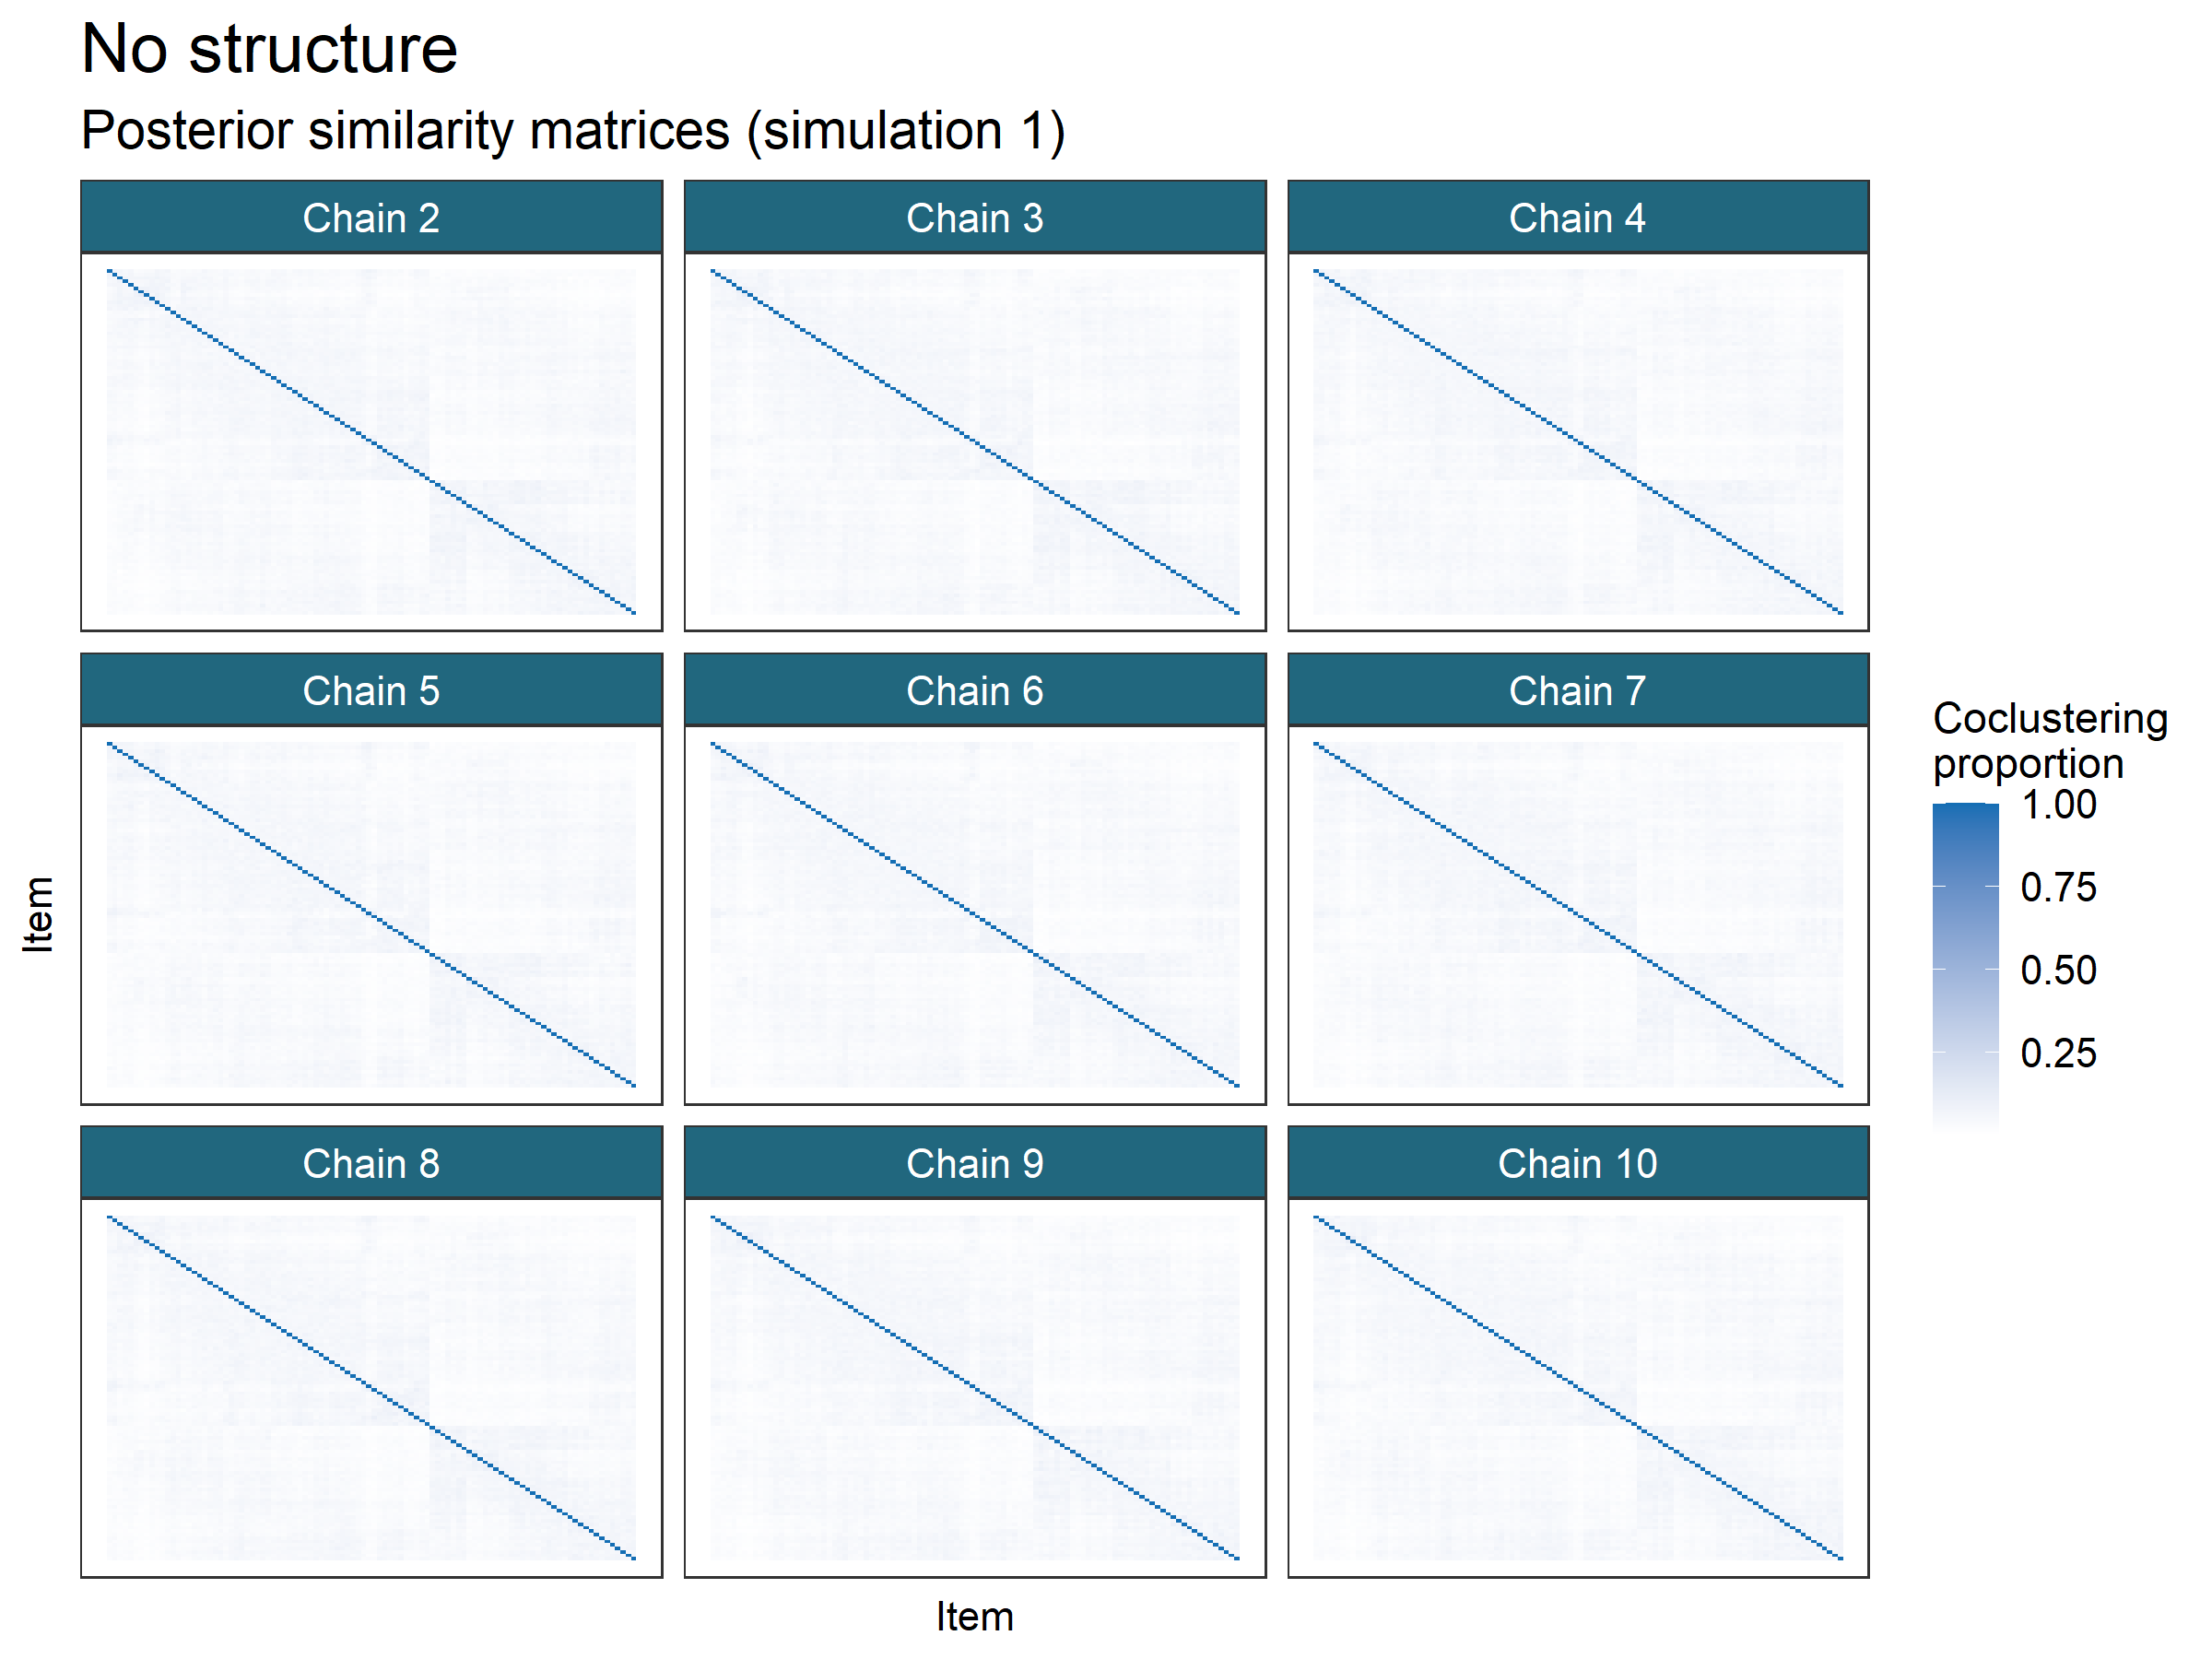
\includegraphics[scale=0.65]{./Images/Simulations/PSMs/no_structureSim1.png}
	\caption{Posterior similarity matrices for simulation 1 of the \emph{No structure} scenario. Each item is allocated to a singleton.}
	\label{fig:simNoStructPSMs}
\end{figure}

\begin{figure} %[!tpb]
	\centering
	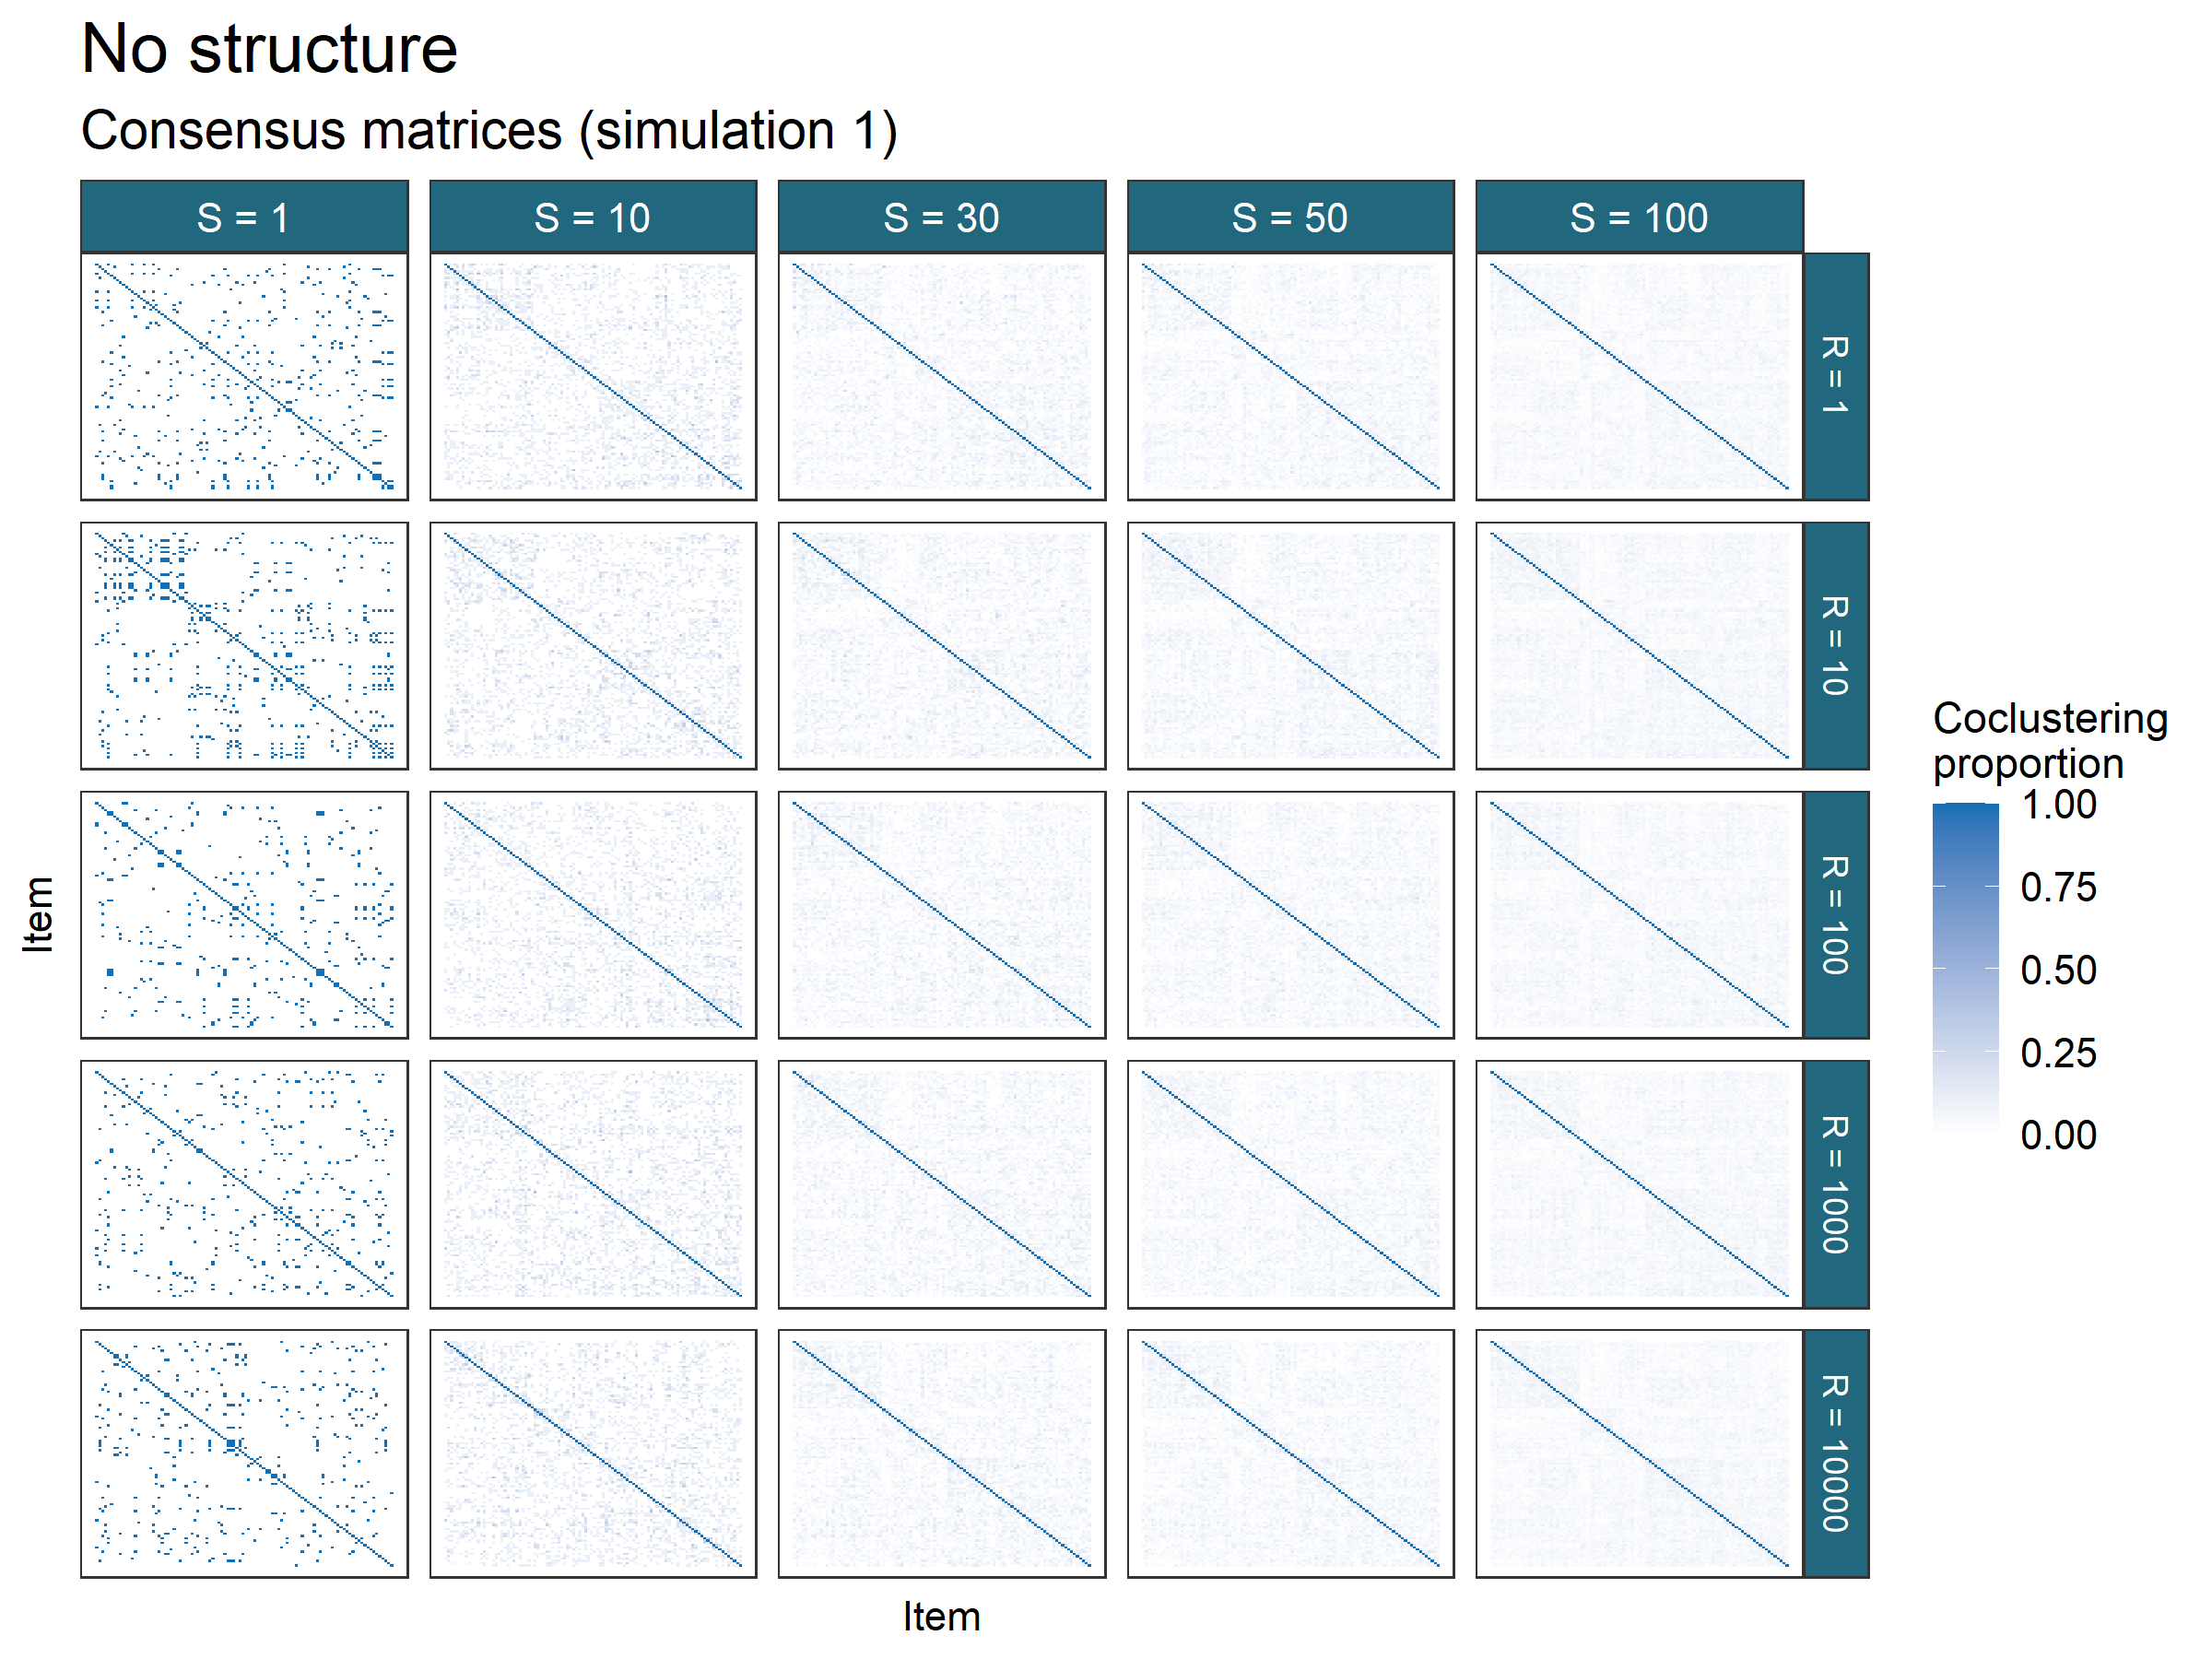
\includegraphics[scale=0.65]{./Images/Simulations/CMs/no_structureSim1.png}
	\caption{Consensus matrices for simulation 1 of the \emph{No structure} scenario. Each item is allocated to a singleton in many of the Consensus matrices.}
	\label{fig:simNoStructCMs}
\end{figure}

Increasing $S$ is also required when the dimensionality of the dataset is large. In this case it is due to individual chains exploring only a single mode (as can be seen in figure \ref{fig:simPSMsDisagreeExample} where each chain appears to sample only a single partition). In this example where each sample is a partition that appears to be a mode in the posterior distribution of the allocation vector from very early in the chain (based upon the stable performance for $R \geq 10$), increasing $S$ allows each chain to ``vote" on which mode is the global mode, as we believe that the mode that attracts the most chains is the global mode (although in real datasets the number of chains required might be greater than in our simulations). An example of this behaviour may be seen in figure \ref{fig:simSmallNLargePCMs}.

\begin{figure} %[!tpb]
	\centering
	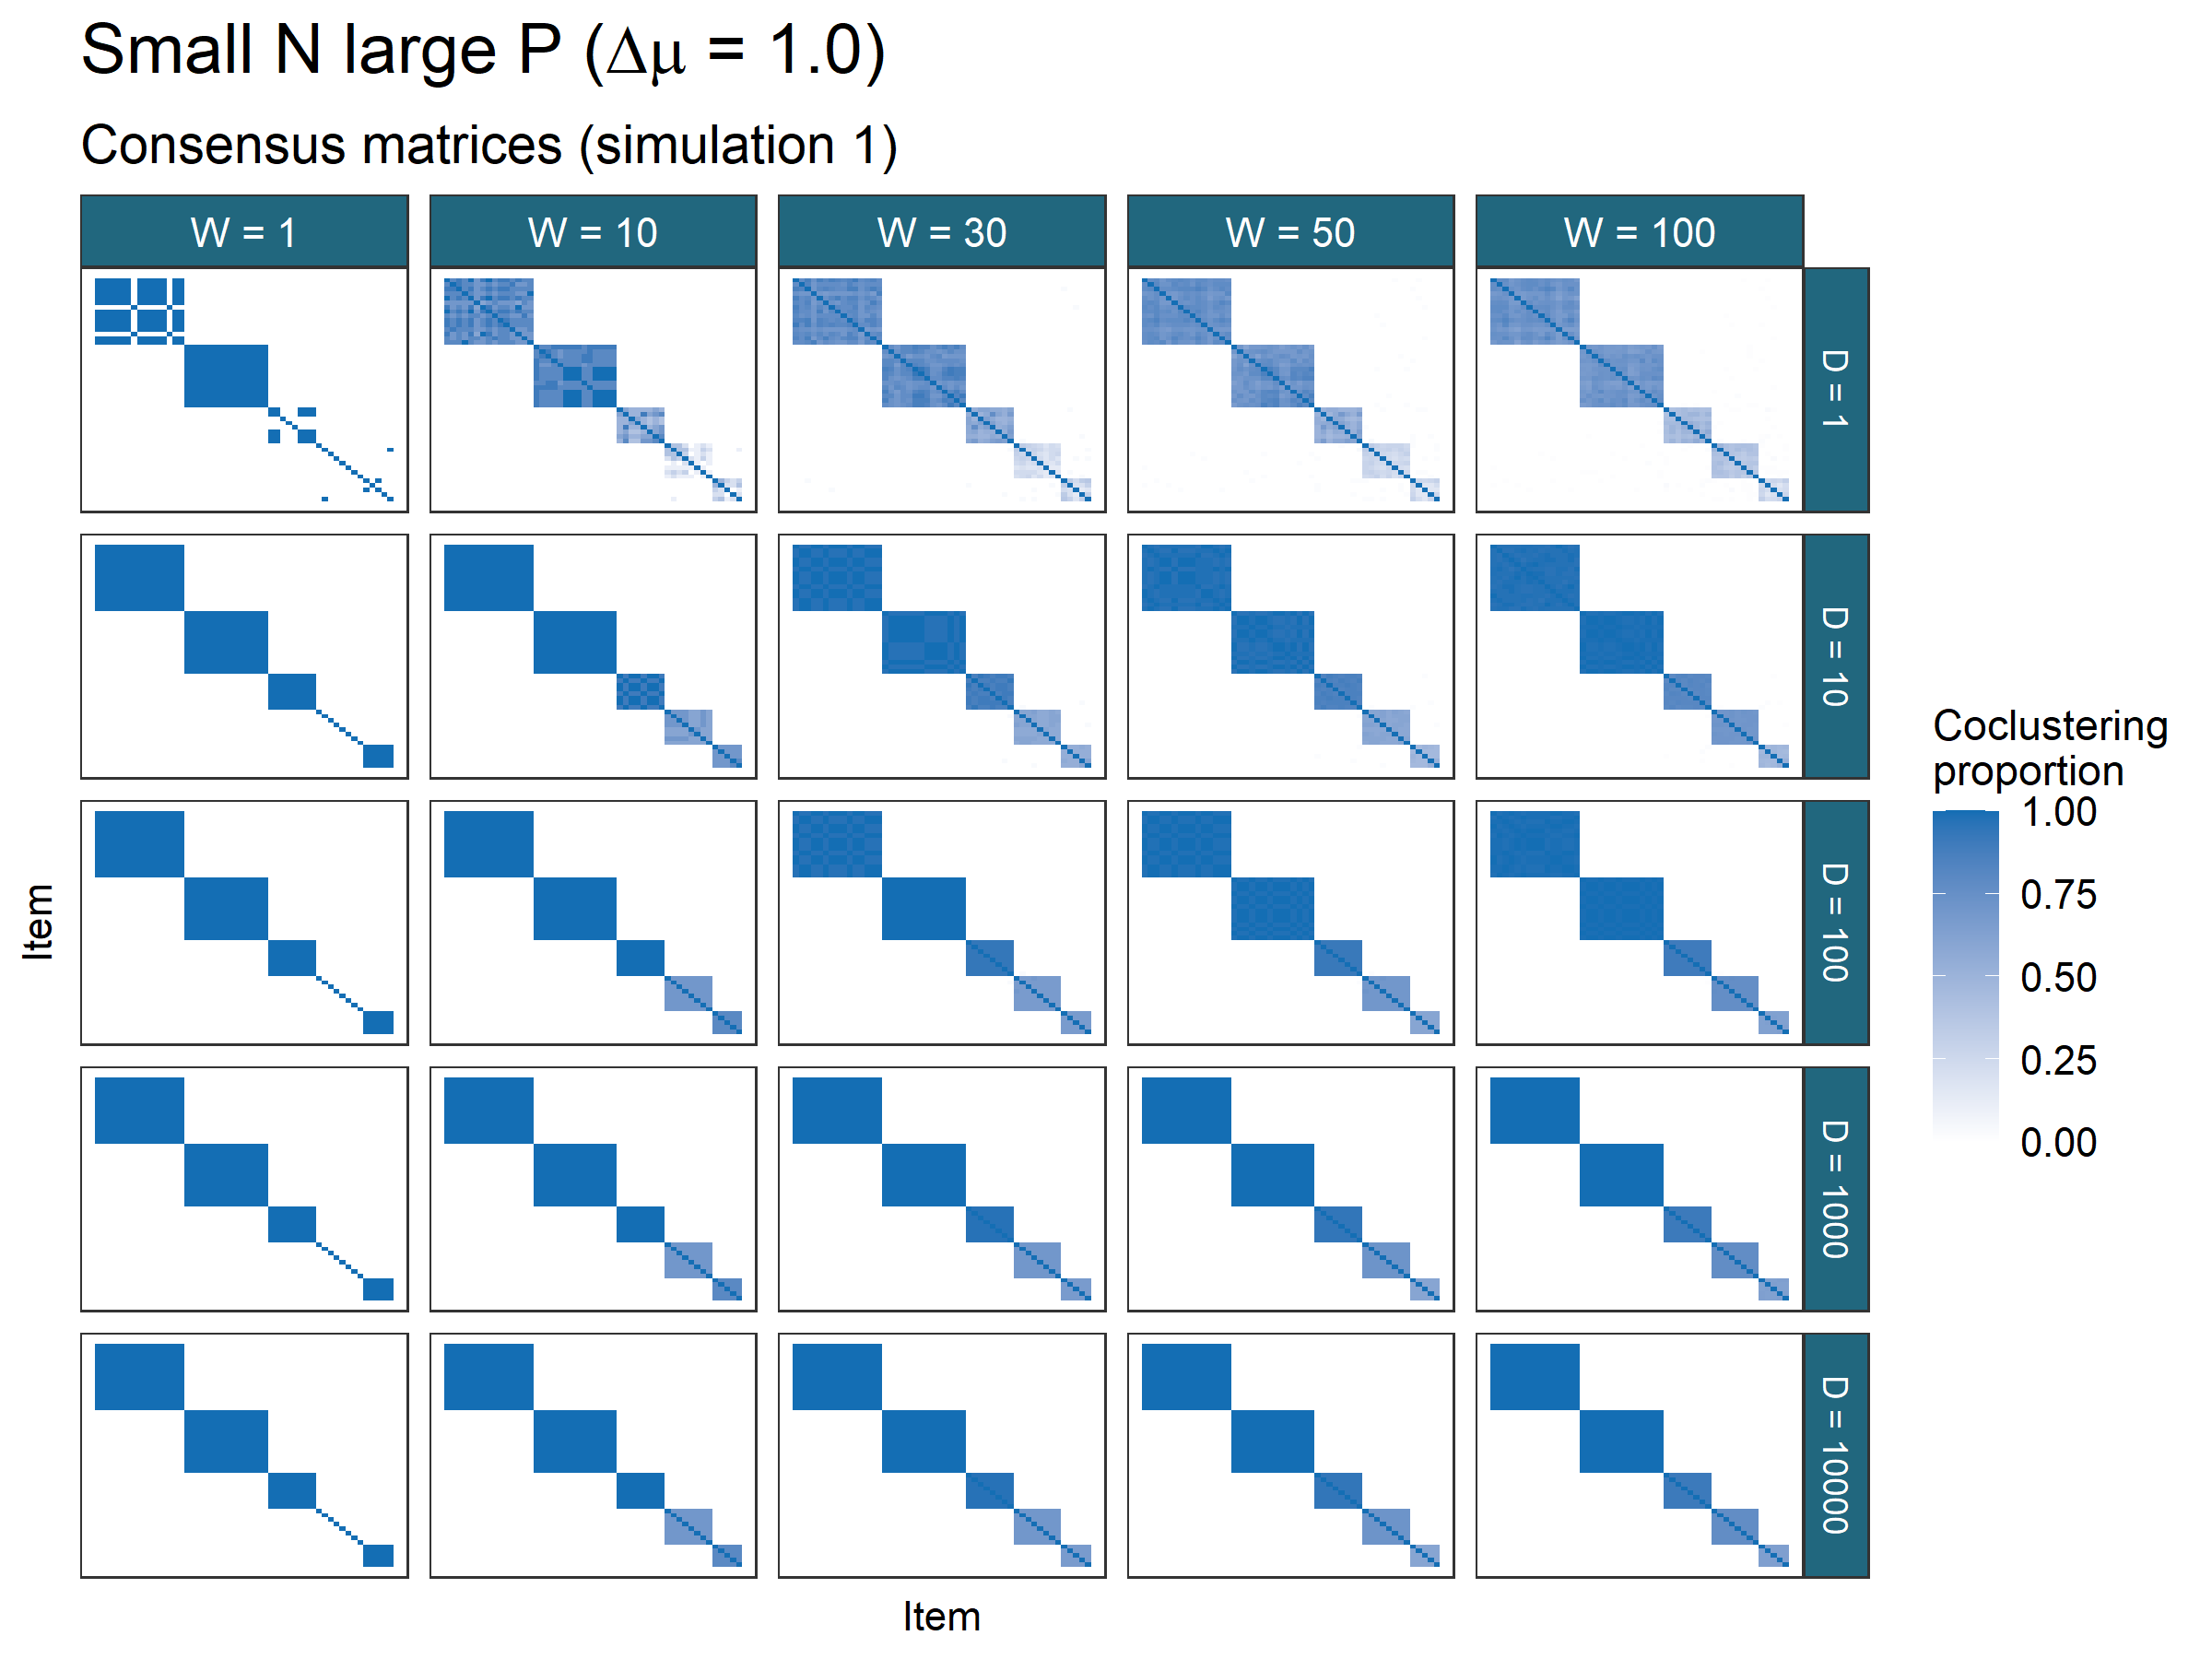
\includegraphics[scale=0.65]{./Images/Simulations/CMs/small_n_large_p_baseSim1.png}
	\caption{Consensus matrices for simulation 1 of the first \emph{Large $N$, small $P$} scenario. One can see that by iteration ten the sample being drawn is from the mode (for $S=1$, $R = 10$), and that an ensemble of chains does find structure that recalls the generating labels (see figure \ref{fig:simPrediction}, the ARI for $CC(10, s)$ is 1.0 for $s > 1$, meaning that the true labels perfectly align with those predicted by the Consensus matrix).}
	\label{fig:simSmallNLargePCMs}
\end{figure}

In figure \ref{fig:simPrediction}, limiting behaviour for increases of $S$ and $R$ can be seen for the ensemble. This inspires our belief that the ensemble depth and width should be grown until this limiting behaviours emerge. In practice where no ground truth is available to compare the ARI values, we recommend visually inspecting the Consensus matrices in a grid like figures \ref{fig:simCMsIrr100}, \ref{fig:simNoStructCMs} and \ref{fig:simSmallNLargePCMs} and checking if there is any noticeable difference between the Consensus matrices for some sets of chain depth, $R'=\{r_1, \ldots, r_a\}$, and chain length $S'=\{s_1, \ldots, s_b\}$ (where $r_i < r_j \iff i < j$ and $s_i < s_j \iff i < j$ for all $i, j$). If there is no difference between the Consensus matrix for $(r_i, s_j)$ and that for $(r_a, s_b)$ for any $i = 1, \ldots, a - 1$, $j = 1, \ldots, b - 1$ than the limiting behaviour is assumed to have emerged. For example, in figure \ref{fig:simSmallNLargePCMs} this limiting behaviour appears to have emerged by $R=10$ and $S=10$, but this can only be seen by comparing the ensembles of $R = 10, S = 30$ and $R=100, S = 10$ with $R= 100, S= 30$. We suggest that $\frac{r_a}{r_{a - 1}} \leq 0.5, \frac{s_b}{s_{b-1}} \leq 0.5$ and $r_a, s_b \geq 50$.

Beyond the empricial behaviour of the ensembles in this simulation study, this heuristic is also inspired by the belief that a clustering method should produce stable results across similar datasets \citep{von2005towards, meinshausen2010stability}. We believe that if the method is still producing a partition that is visibly changing for additional chains and depth, than the random initialisation is influencing the result sufficiently that it is unlikely to be stable for similar datasets or reproducible for a random choice of seeds. % given that is the method is not stable even within the same dataset.

\begin{sidewaysfigure} %[!tpb]
	\centering
	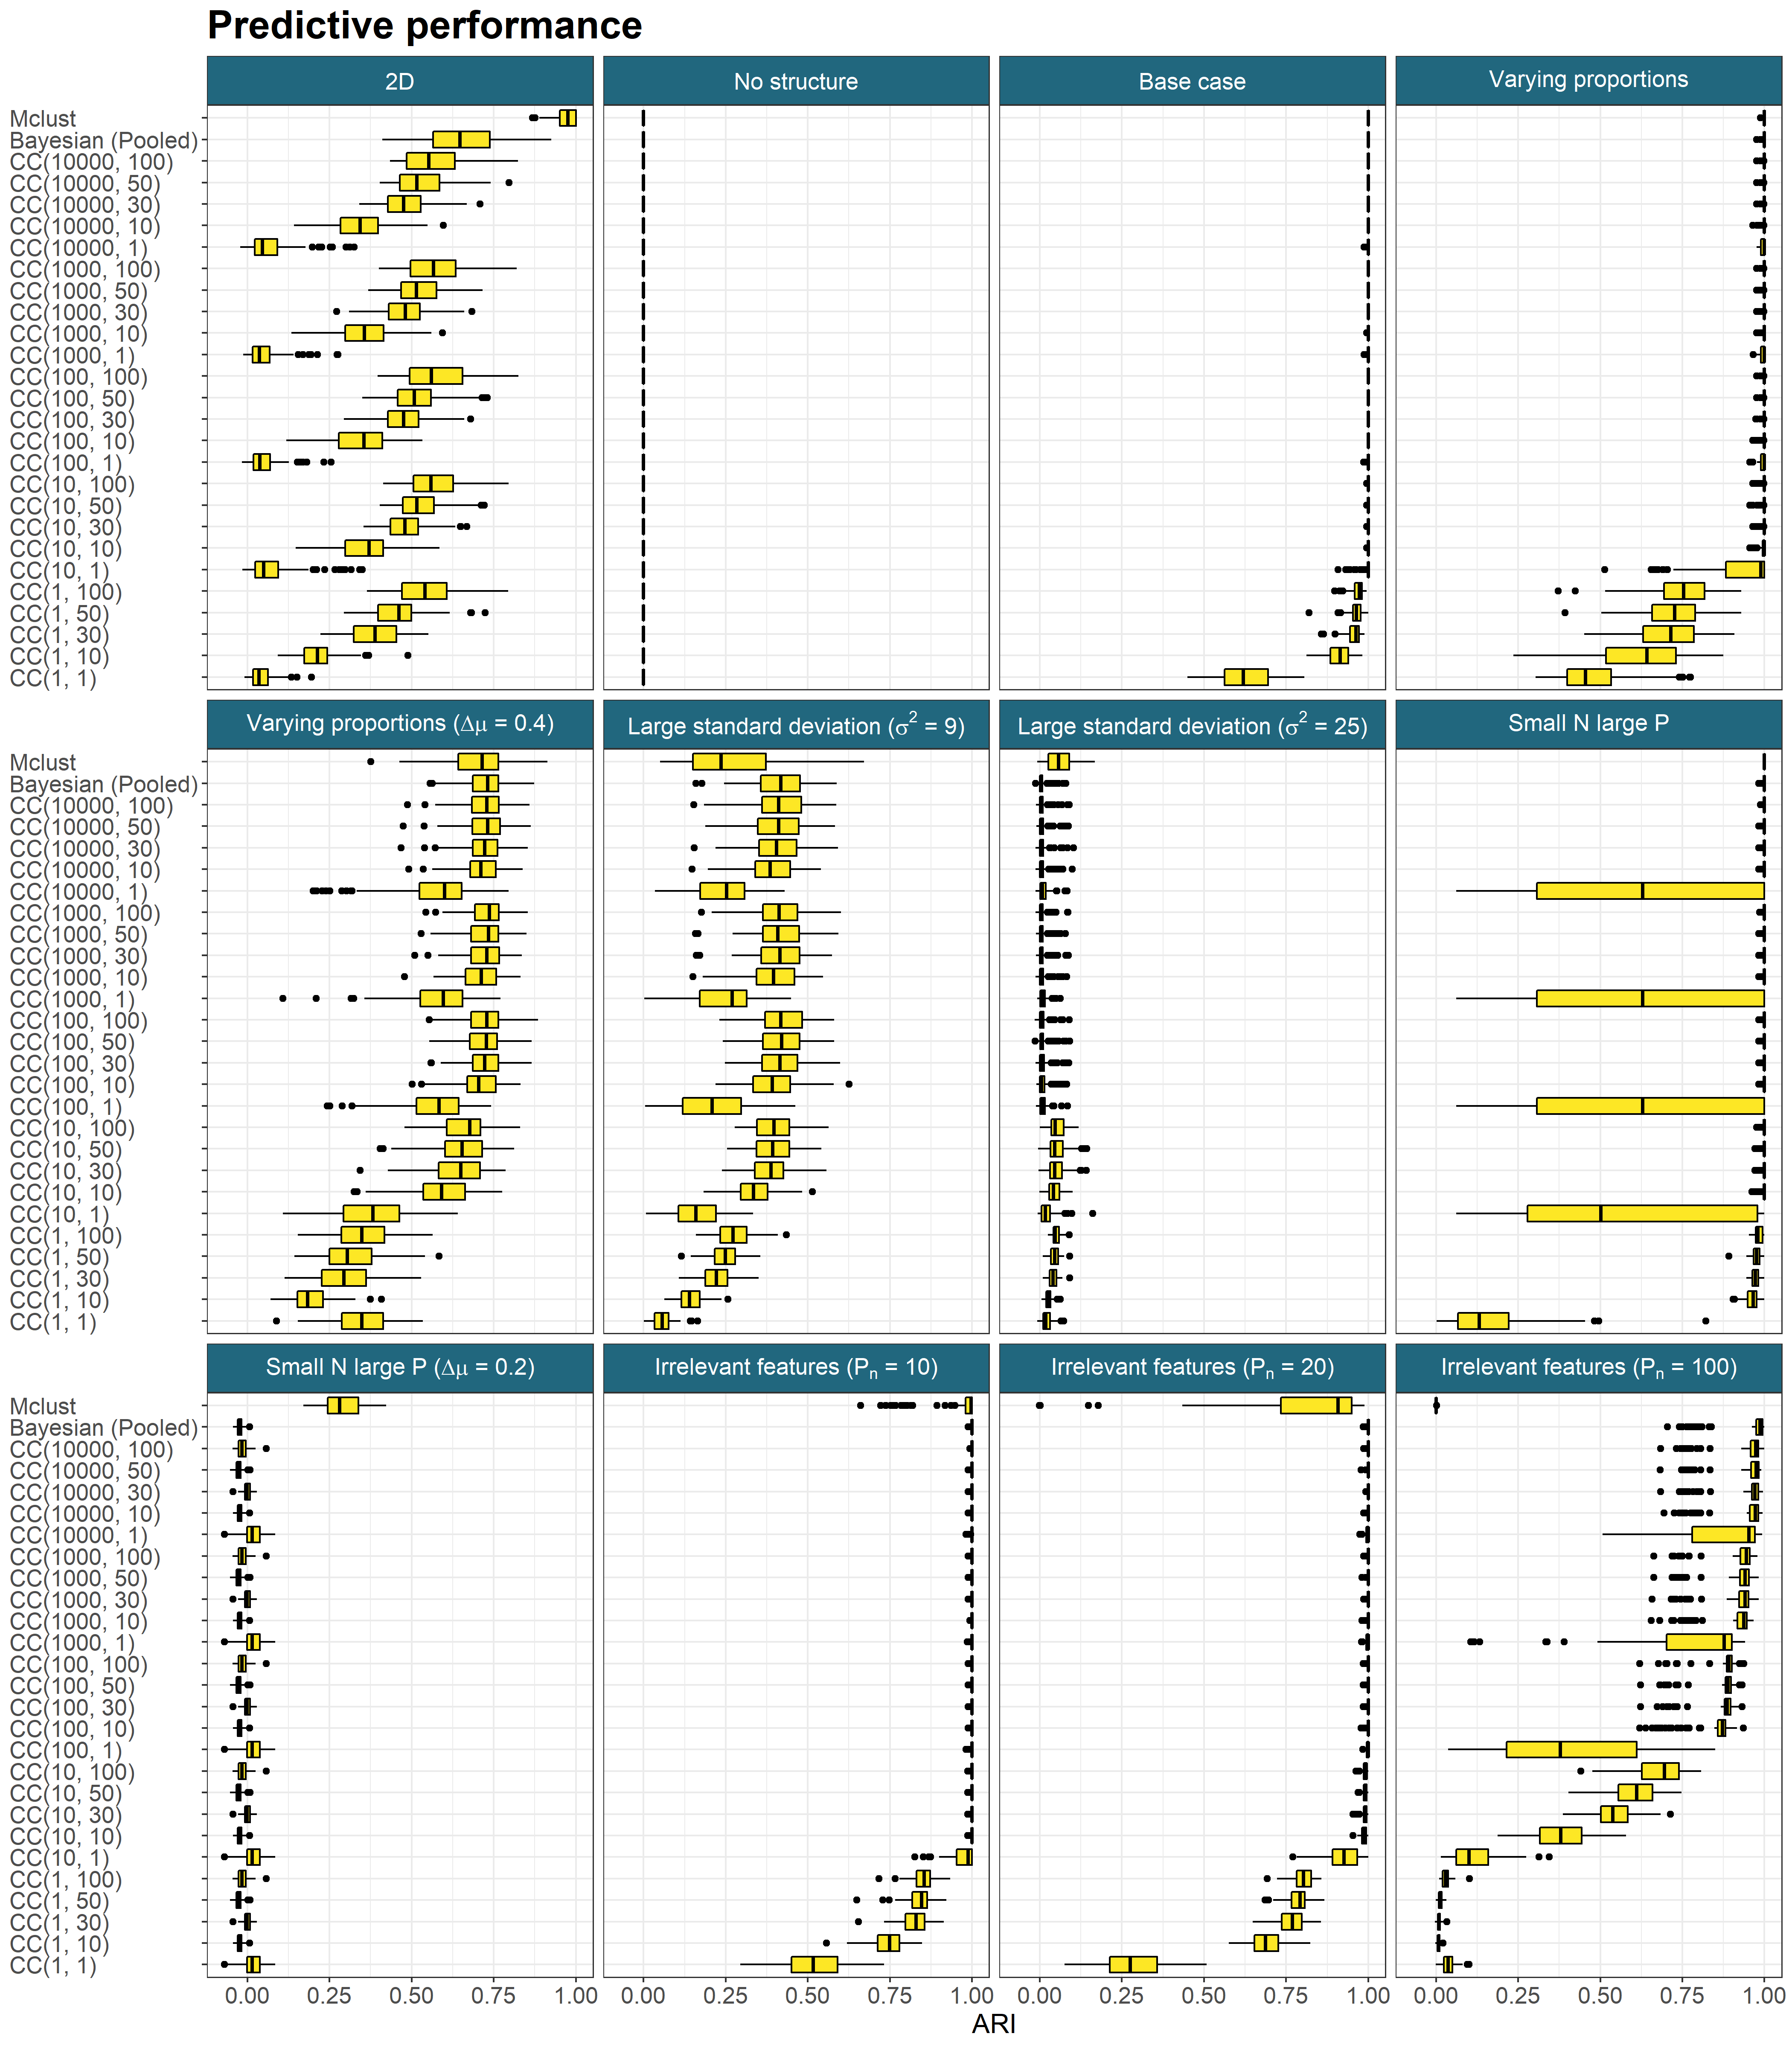
\includegraphics[scale=0.4]{./Images/Simulations/simulation_model_prediction.png}
	\caption{Predictive performance across all simulations. $CC(R, S)$ denotes Consensus clustering using the $R^{th}$ sample from $S$ different chains. In the cases where the generating structure is not exactly found, increasing $R$ and $S$ sees some improvement in the ARI between the truth and the predicted clusterings before some limiting behaviour emerges and and further increase appears to have no change in the performance.}
	\label{fig:simPrediction}
\end{sidewaysfigure}

\begin{sidewaysfigure} %[!tpb]
	\centering
	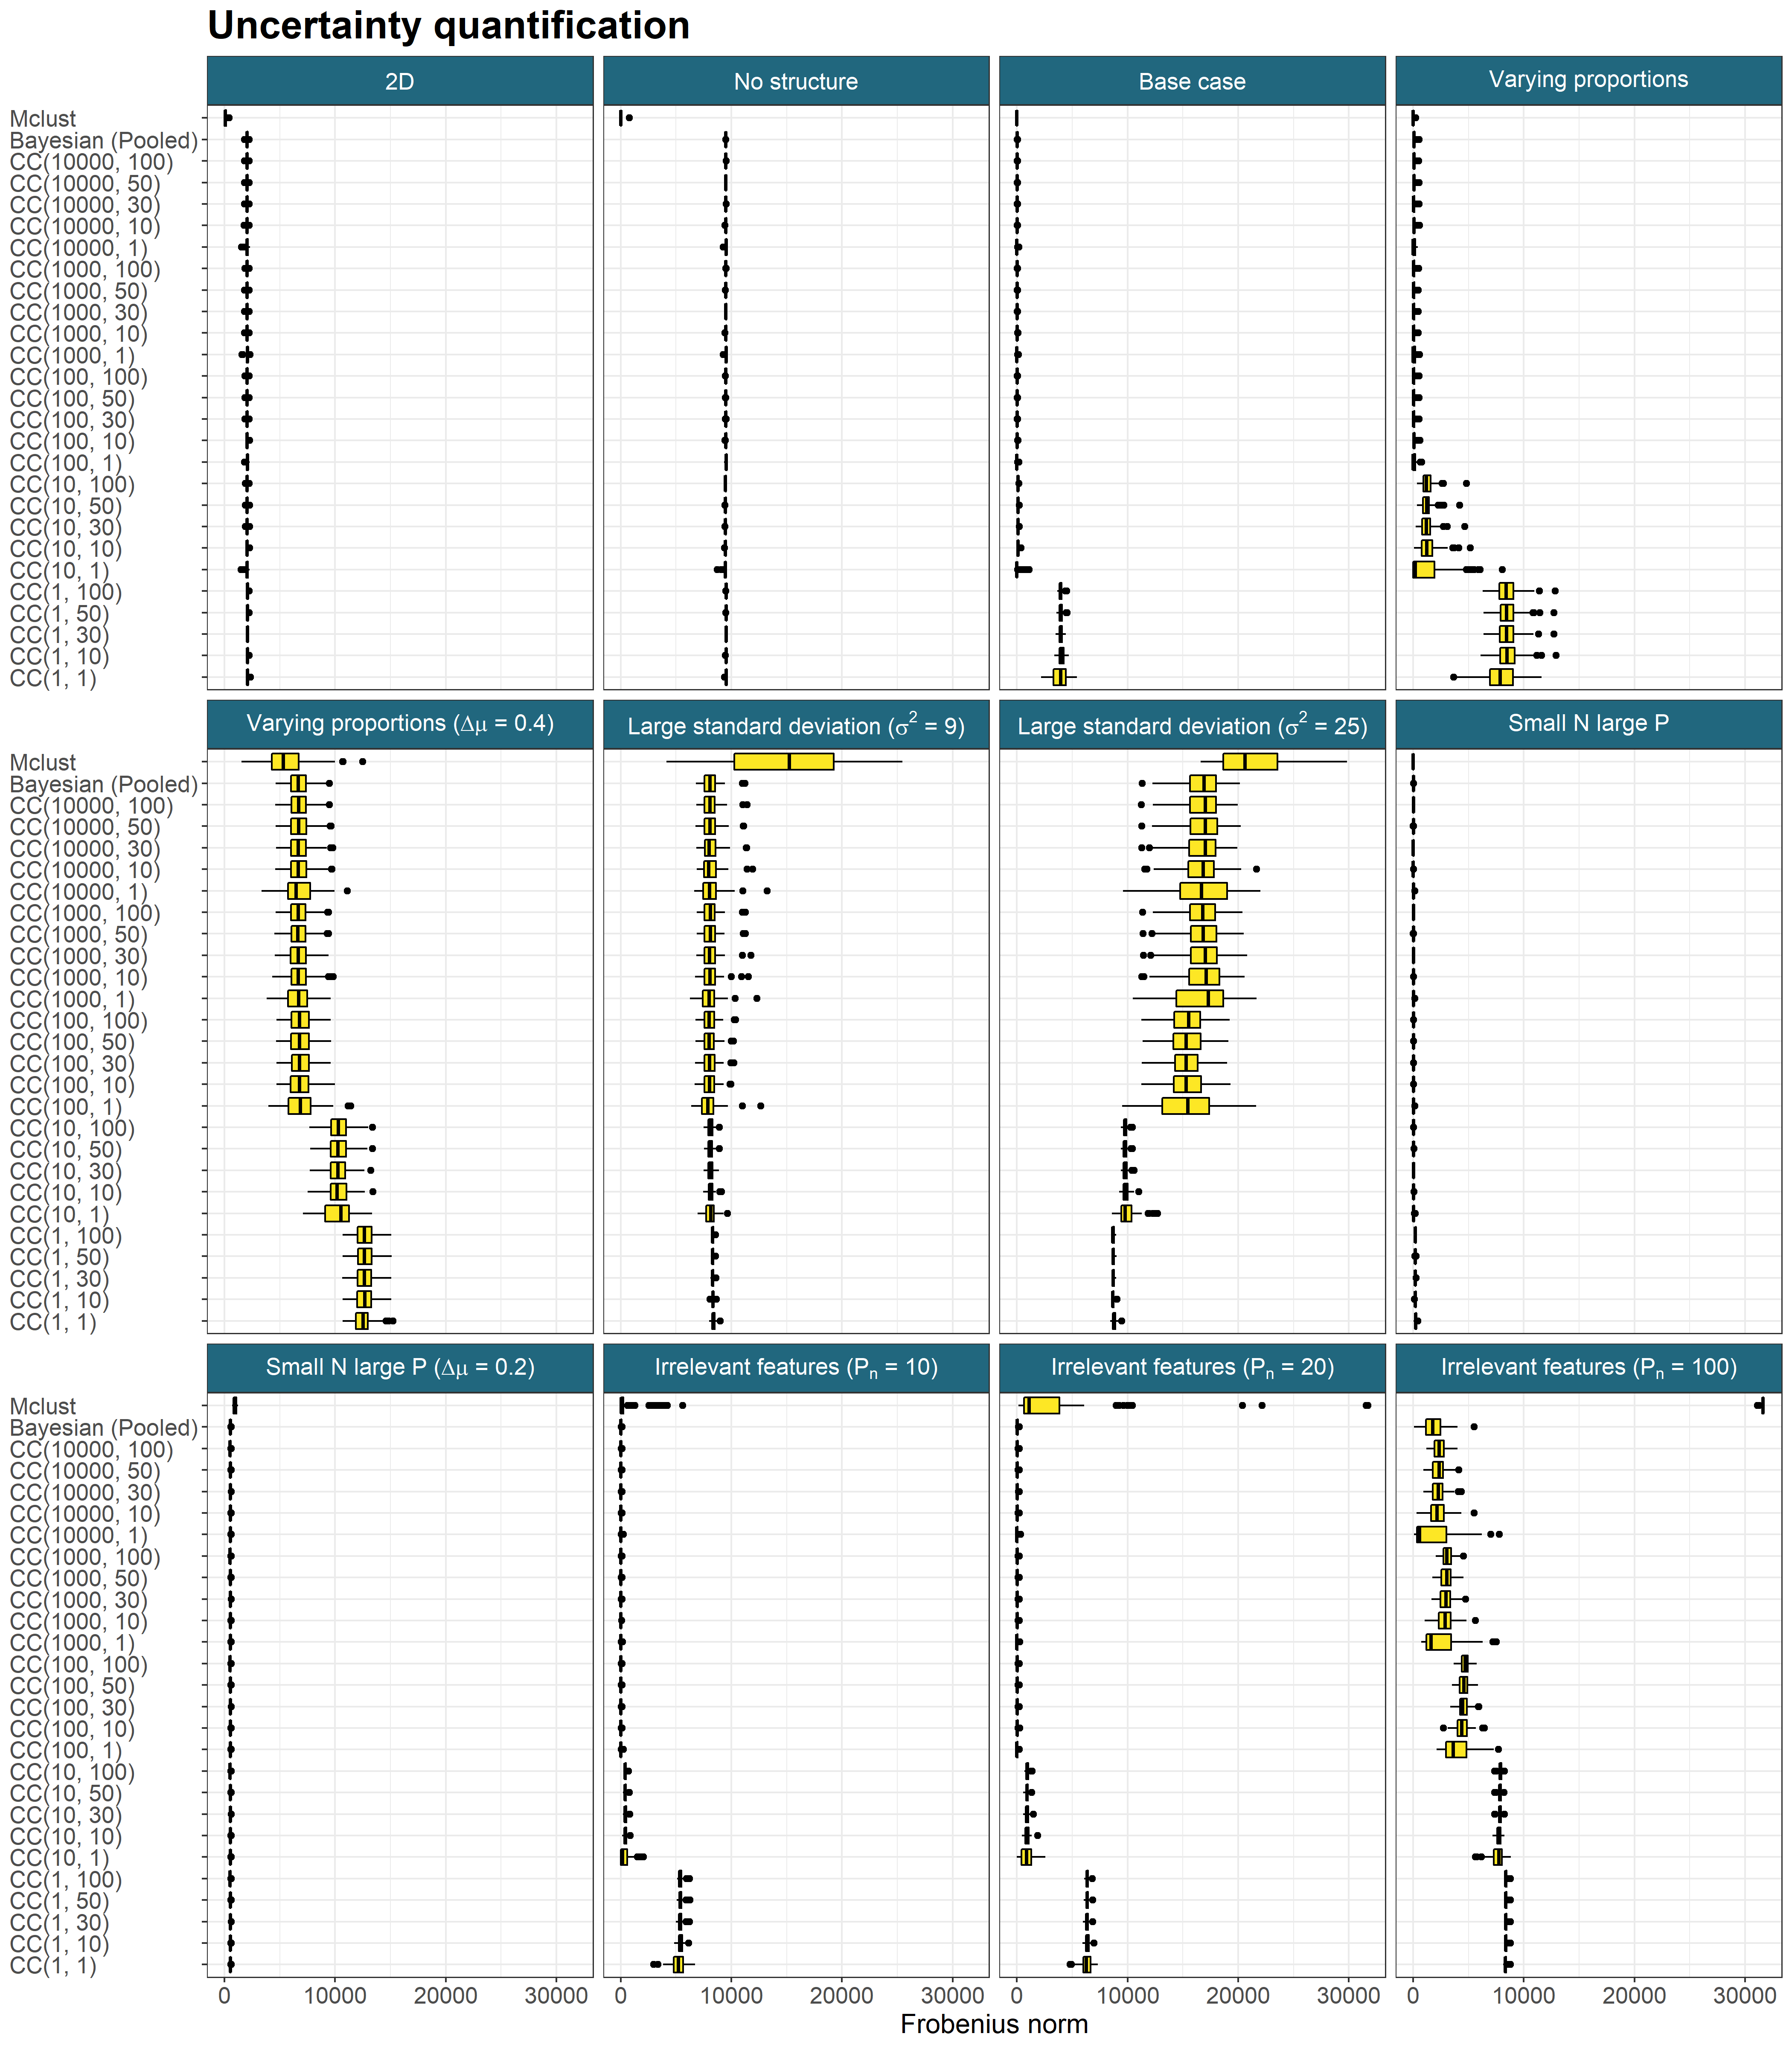
\includegraphics[scale=0.4]{./Images/Simulations/simulation_uncertainty.png}
	\caption{Frobenius norm across simulations. $CC(R, S)$ denotes Consensus clustering using the $R^{th}$ sample from $S$ different chains. Lower values are better. In the \emph{Large standard deivation ($\sigma^2 = 25$)} scenario, the very low valued entries from the ensembles of very short chains are rewarded. These ensembles are not closer to the true structure than the longer ensembles, but they are rewarded for the lack of certainty.}
	\label{fig:simUncertainty}
\end{sidewaysfigure}

\section{Yeast} \label{sec:yeast}

Contents:
\begin{itemize}
	\item Walkthrough datasets (e.g. define protein interactions, what they should tell about gene benefit of co-analysing), 
	\item why co-analyse and 
	\item what info each is expected to contribute.
\end{itemize}

We aimed to construct sets of co-regulated genes that share biological functions in \emph{Saccharomyces cerevisiae}. We believe such informed gene sets are more relevant to phenotypic traits and offer insight into more complex biological processes. To construct these sets we performed an integrative cluster analysis incorporating more biological meaning than a traditional analysis of a single experiment. In the latter case interpreting the clusters defined by similarity within a single experiment often entails strong assumptions about the biological processes behind the result (e.g. correlation of transcripts implies co-regulation).

We included three datasets that are generated using different techniques. We expect that including measurements from a variety of experiments offers more useful information about specific genes and their products than any single type of 'omics data. We performed an integrative analysis of these datasets using the MDI model, jointly modelling the clustering in each dataset. The additional information from the integrative analysis for each gene and the flexible joint model improve our ability to interpret the clusters that emerge as biological constructs without forcing meaning via agressive assumptions or excessive structure \emph{a priori} due to our model choice (e.g. a model that assumes a global generating structure across all datasets).

% We are attempting to learn about higher-level processes that individual genes. To enable this we include more information and use a flexible joint model to improve our ability to interpret the clusters that emerge as biological constructs without forcing \emph{a priori} structure via assumptions (e.g. that co-expressed genes are co-regulated) or our model choice (e.g. a model that assumes a global generating structure across all datasets). Performing individual cluster analyses on each dataset means that 

Our \textbf{Yeast dataset} consists of three datasets with different types of gene products associated with a common set of 551 genes. The datasets are:
\begin{itemize}
	\item microarray profiles of RNA expression from \cite{granovskaia2010high}. This dataset comprises measurements of cell-cycle-regulated expression at 5-minute intervals for 41 time points (up to three cell division cycles) and is referred to as the \textbf{Timecourse} dataset. We include only the genes identified by \cite{granovskaia2010high} as having periodic expression profiles. This includes some non-coding RNAs (\textbf{ncRNAs}) of which the majority are anti-sense RNAs.
	\item Chromatin immunoprecipitation followed by microarray hybridization (\textbf{ChIP-chip}) data from \cite{harbison2004transcriptional}. This dataset has comprises measurements across 117 DNA-binding transcriptional regulators.
	\item Protein-protein interaction (\textbf{PPI}) data from BioGrid \citep{stark2006biogrid}. This dataset consists of of physical and genetic interactions between gene and gene products. The dataset is a collection of results observed in high throughput experiments. The dataset we use contains 603 proteins.
\end{itemize}
The datasets were reduced to 551 items by considering only the genes with no missing data in the PPI and ChIP-chip data. The choices to reduce the datasets to these 551 genes are the same steps as the original MDI paper \citep{kirk2012bayesian}. The data is shown in figure \ref{fig:yeastData}.

Cell-cycle data is exciting as virtually all cellular processes - metabolism, protein synthesis, secretion, DNA replication, organelle biogenesis, cytoskeletal dynamics and chromosome segregation - and diverse regulatory events emerge \cite{granovskaia2010high}. It is also naturally suited to integrative analyis as many of the protein encoding genes in the mitotic cell cycle have well studied genomic binding sites with mapped of transcription factors that control phase-specific expression \citep{cho1998genome, spellman1998comprehensive}. Post-translational regulation also contributes to control of timing of cell-cycle progression in addition to the transcriptional regulation. Thus we hope that for many of our genes that the integration of cell-cycle data, transcription factor data and PPI data should provide rich and meaningful clusters.

We are interested in performing a joint cluster analysis of the three datasets as the shared information will hopefully impart any clusters that emerge across datasets with deeper meaning. For example, if we cluster the Timecourse dataset alone, any clusters that we find are defined by correlation across time. This might be assumed to be driven by shared regulatory mechanisms, but other sources of structure might be encouraging this, even experimental error. However, if a cluster aligns across both the Timecourse dataset and the ChIP-chip dataset we can be more certain that these genes are part of some regulatory network; if this cluster also emerges in the PPI dataset we might believe that the genes are co-regulated as part of the formation of some protein complex.

The MDI model allows different clusters to align across datasets but does not enforce a global structure; this means that individual clusters or even genes can align across datasets based upon the evidence present in the data without forcing global alignment. Thus we can include the PPI data and expect it to contribute to our final clustering despite the expectation that the ncRNAs might not have common cluster allocation across the Timecourse and PPI datasets.

We expect that the complexity of this data and model means that the time required for convergence of the MCMC algorithm would be very large. We avoid this problem by using Consensus clustering of MDI, instead basing our final ensemble choice on the stopping rule laid out in section \ref{sec:stopping}.

The datasets were modelled using a mixture of Gaussian processes in the Timecourse dataset and Multinomial distributions in the ChIP-chip and PPI datasets. To ensure that our mixture model is initially overfitted we set $K_{max}=275\approx\frac{N}{2}$.

\begin{figure}
	\centering
	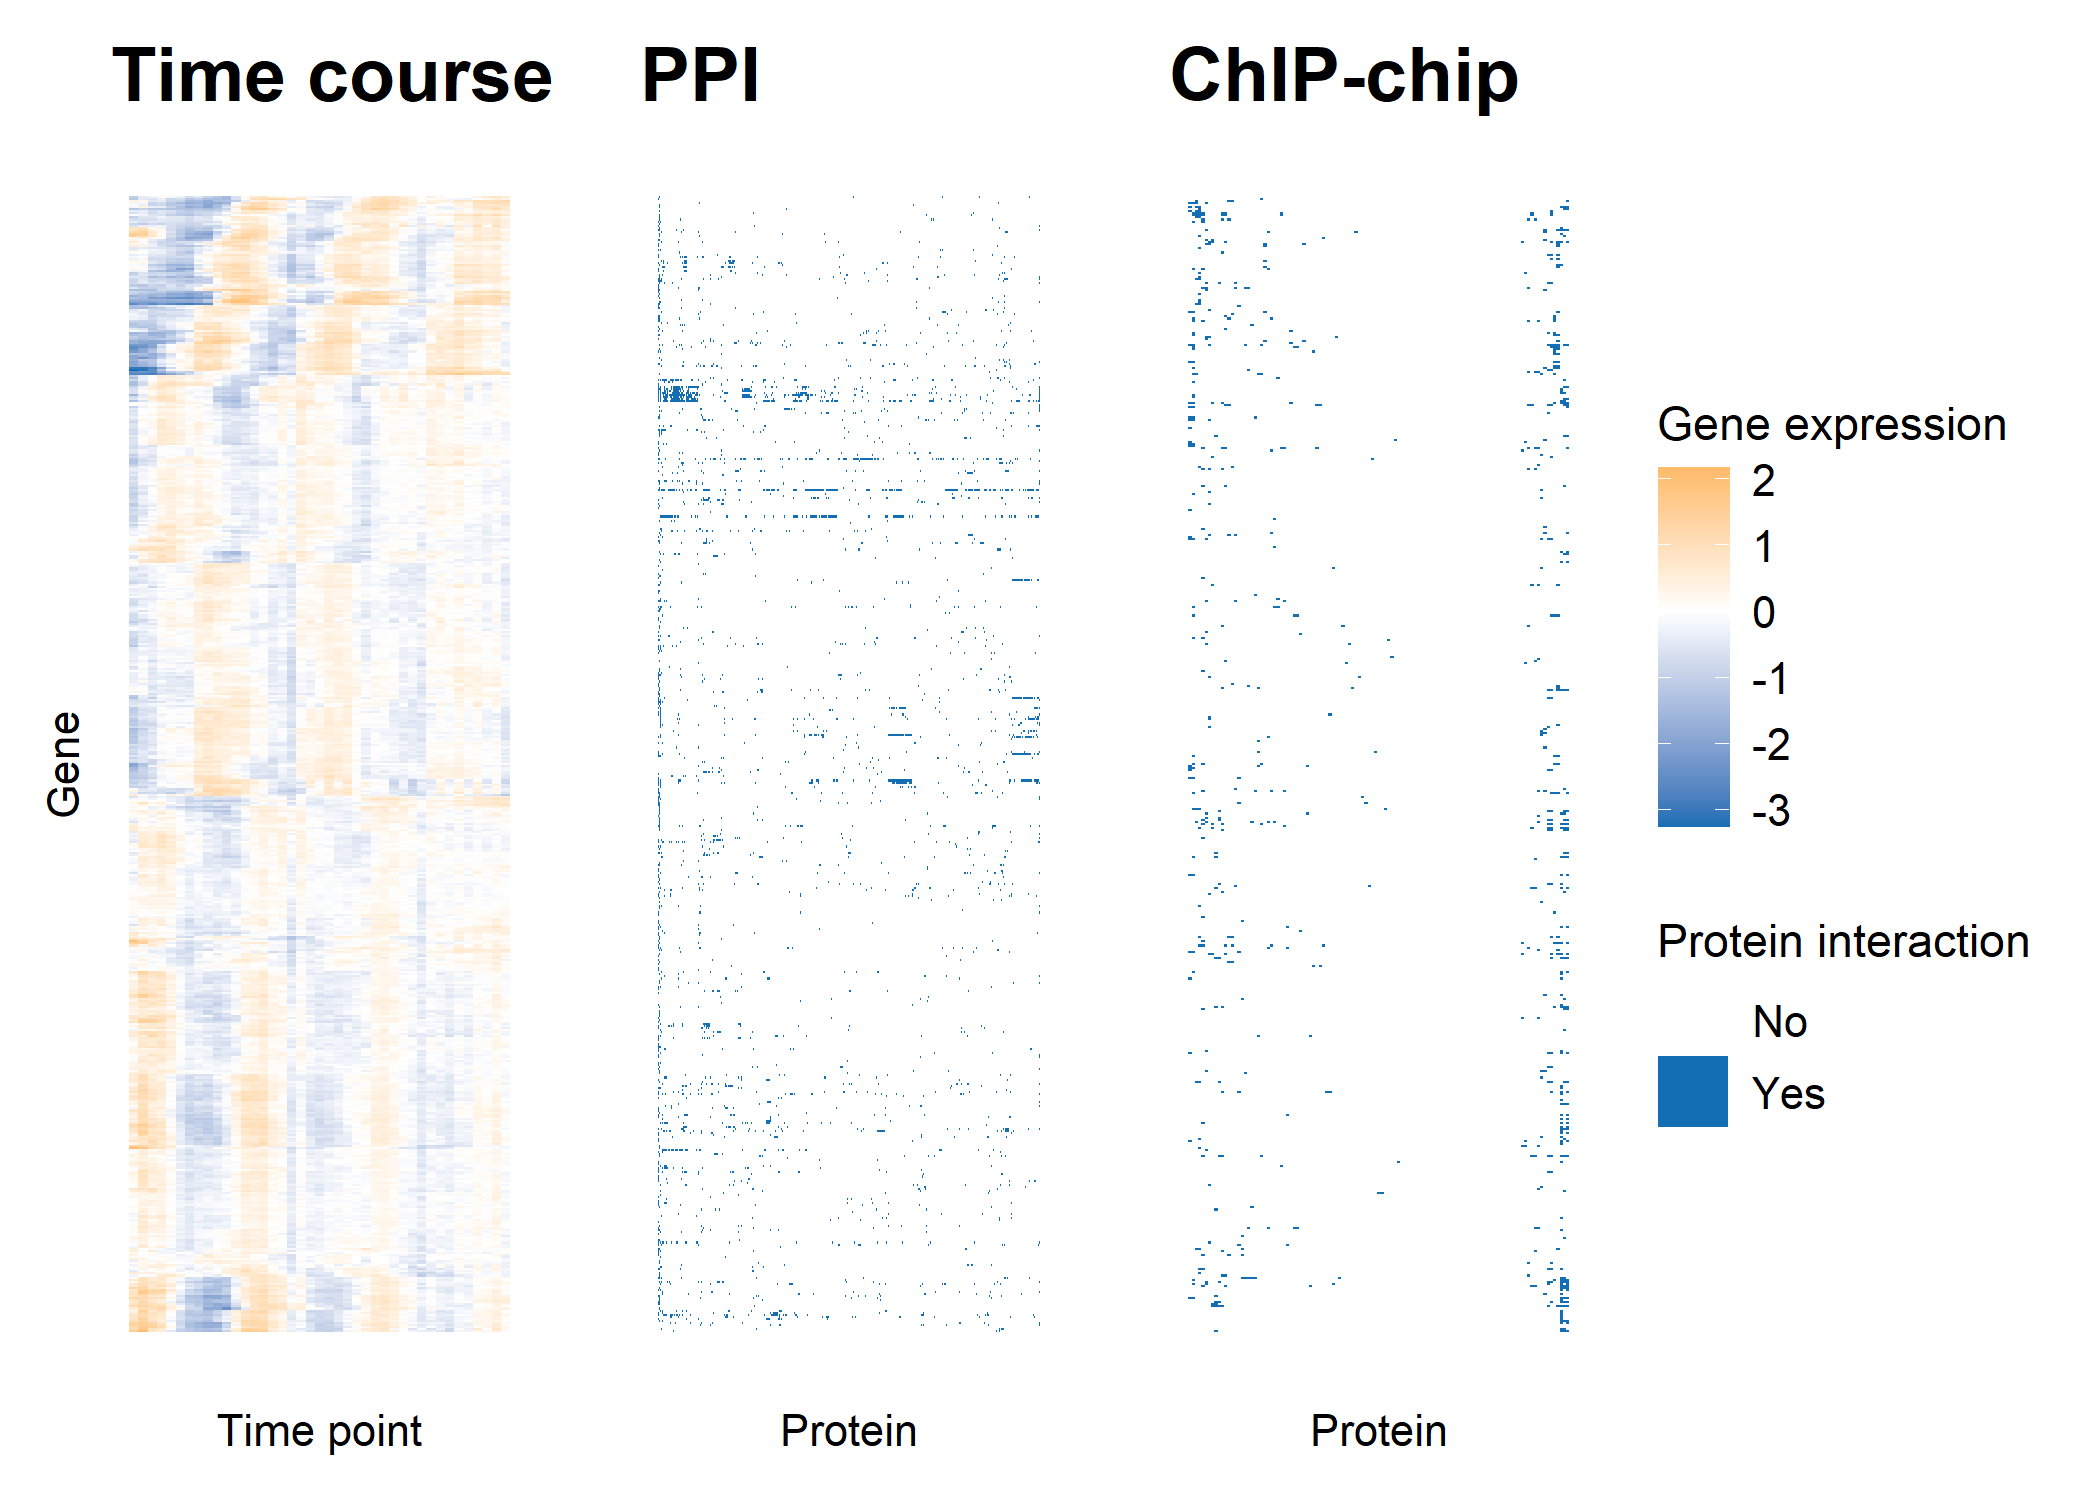
\includegraphics[scale=0.7]{./Images/Yeast/yeastData.png}
	\caption{Heatmap of the yeast datasets. Each plot has a common row order corresponding to the gene products being clustered. This order was decided by a hierarchical clustering of the rows of the Timecourse expression matrix. The Timecourse data is associated with the ``Gene expression" legend and the ChIP-chip and PPI data with ``Protein interaction" legend.}
	\label{fig:yeastData}
\end{figure}

\subsection{Consensus clustering analysis} \label{sec:consensusClustering}

Contents:
\begin{itemize}
	\item Talk about clusters that emerge, number of clusters, similarity across datasets,
	\item Do full analysis via Consensus clustering and then compare to the long chains (comparison separately).
	\item Cluster X is a cluster of genes involved in function Y – look at gene names and gene descriptions.
%	\item Take clusters more than 5 – increases power 
	\item Talk about alignment across datasets.
	\item If ChIP-chip are contributing to timecourse, maybe know which regulate – something is controlling the periodic expression.
\end{itemize}

\subsubsection{Ensemble choice}
We use an ensemble of depth $R=10001$ and width $S=1000$ with a base learner of MDI (using the implementation from \cite{mason2016mdi}). This ensemble depth and width was decided using the stopping rule from section \ref{sec:stopping}. We include the Consensus matrices for this ensemble and those for the combinations of $R = (1001, 5001, 10001)$, $S=(100, 500, 1,000)$ in the three datasets (shown in figures \ref{fig:timecourseCMs}, \ref{fig:chipchipCMs} and \ref{fig:ppiCMs}).

%Following the logic inspired by the behaviour seen in section \ref{sec:simModelPerformance}, we decide the ensemble is sufficiently deep and wide to stop growing if,  for a given depth $r$ and width $s$, there is no visible difference between the Consensus matrices from the ensembles using $R=(a r, r)$, $S=(s, b s)$. In our analysis we used $a=b=0.5$ (the smaller the choice of $a,b$ the more extreme the stopping criterion). An example of this logic can be seen in figures \ref{fig:chipchipCMs} and \ref{fig:ppiCMs} (and to a lesser degree in figure \ref{fig:timecourseCMs}). 

We decide to stop increasing at $R=10001$ as there is no apparent gain in increasing chain depth from $R=5001$ to $R=10001$ across the three datasets. An example of insufficient depth can be see for $R=1001$ in figure \ref{fig:ppiCMs}; there is a marked difference in the Consensus matrices between $R=1001$ and $R=5001$. 

In terms of the number of chains required, we believe this to have stabilised, as there is no obvious change in increasing $S$ from 100 in any dataset.

\subsection{Cluster analysis}
We use \texttt{maxpear} to infer an estimate clustering from the Consensus matrices as in the Simulations except we set \texttt{k.max = 275}. 

% Table created by stargazer v.5.2.2 by Marek Hlavac, Harvard University. E-mail: hlavac at fas.harvard.edu
% Date and time: Tue, Oct 27, 2020 - 15:28:31

%\begin{table}[!htbp] \centering 
%	\caption{} 
%	\label{} 

\subsubsection{Fused genes}
\begin{itemize}
	\item Cluster 1: NAD+ Metabolism and Regulation
	\item Cluster 2: singleton
	\item Cluster 3: G1 arrest / S-phase initiation \citep{schwob1993clb5, stuart1998clb5, crosby2007cell, chang2017yeast, miles2016msa1};
	\item Cluster 4: 
\end{itemize}


	\begin{longtable}{@{\extracolsep{3pt}} cccp{85mm}} 
		\\[-1.8ex]\hline 
		\hline \\[-1.8ex] 
		ORF & Gene & Cluster & Description \\ 
		\hline \\[-1.8ex] 
		YOR374W & ALD4 & 1 & Mitochondrial aldehyde dehydrogenase;
%		required for growth on ethanol and conversion of acetaldehyde to acetate; 
		phosphorylated; activity is K+ dependent; utilizes NADP+ or NAD+ equally as coenzymes; expression is glucose repressed 
%		can substitute for cytosolic NADP-dependent aldehyde dehydrogenase when directed to the cytosol; human homolog ALDH2 can complement yeast ald4 mutant
		\\ 
		YGL037C & PNC1 & 1 & Nicotinamidase that converts nicotinamide to nicotinic acid; part of the NAD(+) salvage pathway
%		; required for life span extension by calorie restriction; lacks a peroxisomal targeting signal but is imported into peroxisomes via binding to Gpd1p; PNC1 expression responds to all known stimuli that extend replicative life span; protein increases in abundance and relative distribution to cytoplasmic foci decreases upon DNA replication stress
		\\ 
		YCL040W & GLK1 & 1 & Glucokinase; catalyzes the phosphorylation of glucose at C6 in the first irreversible step of glucose metabolism; one of three glucose phosphorylating enzymes
%		; expression regulated by non-fermentable carbon sources; GLK1 has a paralog, EMI2, that arose from the whole genome duplication 
		\\  \hline \\ [-1.8ex] 
		YBL010C &  & 2 & Putative protein of unknown function; green fluorescent protein (GFP)-fusion protein colocalizes with clathrin-coated vesicles \\  \hline \\ [-1.8ex] 
		YKR077W & MSA2 & 3 & Modulates G1-specific transcription to promote G1 arrest \citep{miles2016msa1}; 
		Putative transcriptional activator; interacts with G1-specific transcription factor MBF and G1-specific promoters; MSA2 has a paralog, MSA1, that arose from the whole genome duplication \\
		YPL014W & CIP1 & 3 & Cyclin-dependent kinase inhibitor; interacts with and inhibits the Cdc28p/Cln2p, G1/S phase cyclin-dependent kinase complex but not S-phase, or M-phase complexes; overexpression blocks cells in G1 phase and stabilizes the Cdc28p inhibitor Sic1p, while disruption accelerates the G1/S phase transition; phosphorylated during S phase in a Cdc28p-dependent manner
%		; green fluorescent protein (GFP)-fusion protein localizes to the cytoplasm and to the nucleus 
		\\ 
		YGR109C & CLB6 & 3 & B-type cyclin involved in DNA replication during S phase; activates Cdc28p to promote initiation of DNA synthesis; functions in formation of mitotic spindles along with Clb3p and Clb4p; most abundant during late G1
%		; CLB6 has a paralog, CLB5, that arose from the whole genome duplication 
		\\  \hline \\ [-1.8ex] 
		YNL310C & ZIM17 & 4 & 
		Protein co-chaperone with a zinc finger motif; 
		essential for protein import into mitochondria; 
		may act with Pam18p to facilitate recognition and folding of imported proteins by Ssc1p (mtHSP70) in the mitochondrial matrix; 
		required for the maintenance of Ssc1p solubility and assists in the functional interaction of Ssc1p with substrate proteins \\ 
		YML020W &  & 4 & Putative protein of unknown function \\ 
		YHR159W & TDA11 & 4 & Putative protein of unknown function; green fluorescent protein (GFP)-fusion protein localizes to the cytoplasm %; 
%		potential Cdc28p substrate; null mutant is sensitive to expression of the top1-T722A allele 
		\\ 
		YJR154W &  & 4 & Putative protein of unknown function; green fluorescent protein (GFP)-fusion protein localizes to the cytoplasm \\ 
		YBR073W & RDH54 & 4 & DNA-dependent ATPase; DNA recombination/repair translocase, supercoils DNA and promotes DNA strand opening; stimulates strand exchange by modifying dsDNA topology; involved in recombinational repair of DNA double-strand breaks (DSBs) during mitosis and meiosis; phosphorylated in Mec1p-, Rad53p-dependent way in response to one DSB; contributes to remodelling of nucleosomes; proposed to be involved in crossover interference; interacts with Dmc1p; stimulates Dmc1p and Rad51p \\ 
		YER170W & ADK2 & 4 & Mitochondrial adenylate kinase; catalyzes the reversible synthesis of GTP and AMP from GDP and ADP; may serve as a back-up for synthesizing GTP or ADP depending on metabolic conditions; 3' sequence of ADK2 varies with strain background \\  \hline \\ [-1.8ex] 
		YNL165W &  & 5 & Putative protein of unknown function; YNL165W is not an essential gene \\ 
		YIL132C & CSM2 & 5 & Component of Shu complex (aka PCSS complex); Shu complex also includes Psy3, Shu1, Shu2, and promotes error-free DNA repair,; Shu complex mediates inhibition of Srs2p function; promotes formation of Rad51p filaments; Psy3p and Csm2p contain similar DNA-binding regions which work together to form a single DNA binding site; required for accurate chromosome segregation during meiosis \\ 
		YKL165C & MCD4 & 5 & Protein involved in GPI anchor synthesis; multimembrane-spanning protein that localizes to the endoplasmic reticulum; highly conserved among eukaryotes; GPI stands for glycosylphosphatidylinositol \\ 
		YDR518W & EUG1 & 5 & Protein disulfide isomerase of the endoplasmic reticulum lumen; 
%		EUG1 has a paralog, PDI1, that arose from the whole genome duplication; function overlaps with that of Pdi1p; 
		may interact with nascent polypeptides in the ER 
		\\ 
		YGL027C & CWH41 & 5 & Processing alpha glucosidase I; ER type II integral membrane N-glycoprotein involved in assembly of cell wall beta 1,6 glucan and asparagine-linked protein glycosylation; also involved in ER protein quality control and sensing of ER stress \\ 
		YDL093W & PMT5 & 5 & Protein O-mannosyltransferase; transfers mannose residues from dolichyl phosphate-D-mannose to protein serine/threonine residues; acts in a complex with Pmt3p, can instead interact with Pmt2p in some conditions; target for new antifungals \\ 
		YLR151C & PCD1 & 5 & 8-oxo-dGTP diphosphatase; prevents spontaneous mutagenesis via sanitization of oxidized purine nucleoside triphosphates; can also act as peroxisomal pyrophosphatase with specificity for coenzyme A and CoA derivatives, may function to remove potentially toxic oxidized CoA disulfide from peroxisomes to maintain the capacity for beta-oxidation of fatty acids; nudix hydrolase family member; similar E. coli MutT and human, rat and mouse MTH1 \\  \hline \\ [-1.8ex] 
		YPL163C & SVS1 & 6 & Cell wall and vacuolar protein; required for wild-type resistance to vanadate %; SVS1 has a paralog, SRL1, that arose from the whole genome duplication 
		\\  \hline \\ [-1.8ex] 
		YDR400W & URH1 & 7 & Uridine nucleosidase (uridine-cytidine N-ribohydrolase); cleaves N-glycosidic bonds in nucleosides; involved in the pyrimidine salvage and nicotinamide riboside salvage pathways \\ 
		YNL072W & RNH201 & 7 & Ribonuclease H2 catalytic subunit; removes RNA primers during Okazaki fragment synthesis and errant ribonucleotides misincorporated during DNA replication; role in ribonucleotide excision repair; homolog of RNAse HI; related to human AGS4 which causes Aicardi-Goutieres syndrome \\ 
		YOL019W &  & 7 & Protein of unknown function; green fluorescent protein (GFP)-fusion protein localizes to the cell periphery and vacuole; YOL019W has a paralog, DCV1, that arose from the whole genome duplication \\ 
		YDL010W & GRX6 & 7 & Cis-golgi localized monothiol glutaredoxin, binds Fe-S cluster; more similar in activity to dithiol than other monothiol glutaredoxins; involved in the oxidative stress response; GRX6 has a paralog, GRX7, that arose from the whole genome duplication \\ 
		YDL211C &  & 7 & Protein of unknown function; green fluorescent protein (GFP)-fusion protein localizes to the vacuole; YDL211C has a paralog, TDA7, that arose from the whole genome duplication \\  \hline \\ [-1.8ex] 
		YDR356W & SPC110 & 8 & Inner plaque spindle pole body (SPB) component; ortholog of human kendrin; gamma-tubulin small complex (gamma-TuSC) receptor that interacts with Spc98p to recruit the complex to the nuclear side of the SPB, connecting nuclear microtubules to the SPB; promotes gamma-TuSC assembly and oligomerization to initiate microtubule nucleation; interacts with Tub4p-complex and calmodulin; phosphorylated by Mps1p in cell cycle-dependent manner \\ 
		YHR172W & SPC97 & 8 & Component of the microtubule-nucleating Tub4p (gamma-tubulin) complex; interacts with Spc110p at the spindle pole body (SPB) inner plaque and with Spc72p at the SPB outer plaque \\  \hline \\ [-1.8ex] 
		YDR389W & SAC7 & 9 & GTPase activating protein (GAP) for Rho1p; regulator of a Tor2p-mediated, Rho1p GTPase switch that controls organization of the actin cytoskeleton; negative regulator of the RHO1-PKC1-MAPK cell integrity (CWI) and membrane fluidity homeostasis signaling pathways; potential Cdc28p substrate; SAC7 has a paralog, BAG7, that arose from the whole genome duplication \\  \hline \\ [-1.8ex] 
		YBR242W &  & 10 & Putative protein of unknown function; green fluorescent protein (GFP)-fusion protein localizes to the cytoplasm and nucleus; YBR242W is not an essential gene; YBR242W has a paralog, YGL101W, that arose from the whole genome duplication \\ 
		YOR104W & PIN2 & 10 & Exomer-dependent cargo protein; induces appearance of [PIN+] prion when overproduced; prion-like domain serves as a retention signal in the trans-Golgi network; predicted to be palmitoylated \\ 
		YDR514C &  & 10 & Protein of unknown function that localizes to mitochondria; overexpression affects endocytic protein trafficking; YDR514C has a paralog, GFD2, that arose from the whole genome duplication \\ 
		YLL028W & TPO1 & 10 & Polyamine transporter of the major facilitator superfamily; member of the 12-spanner drug:H(+) antiporter DHA1 family; recognizes spermine, putrescine, and spermidine; catalyzes uptake of polyamines at alkaline pH and excretion at acidic pH; during oxidative stress exports spermine, spermidine from the cell, which controls timing of expression of stress-responsive genes; phosphorylation enhances activity and sorting to the plasma membrane \\ 
		YNL024C & EFM6 & 10 & Putative S-adenosylmethionine-dependent lysine methyltransferase; responsible for modifying Lys-390 in translational elongation factor EF-1 alpha (eEF1A); has seven beta-strand methyltransferase motif; green fluorescent protein (GFP)-fusion protein localizes to the cytoplasm \\ 
		YCR024C-A & PMP1 & 10 & Regulatory subunit for the plasma membrane H(+)-ATPase Pma1p; small single-membrane span proteolipid; forms unique helix and positively charged cytoplasmic domain that is able to specifically segregate phosphatidylserines; PMP1 has a paralog, PMP2, that arose from the whole genome duplication \\ 
		YNR004W & SWM2 & 10 & Protein with a role in snRNA and snoRNA cap trimethylation; interacts with Tgs1p and shows similar phenotypes; required for trimethylation of the caps of spliceosomal snRNAs and the U3 snoRNA, and for efficient 3' end processing of U3 snoRNA; may act as a specificity factor for Tgs1p \\ 
		YDR020C & DAS2 & 10 & Putative protein of unknown function; non-essential gene identified in a screen for mutants with increased levels of rDNA transcription; weak similarity with uridine kinases and with phosphoribokinases \\ 
		YER140W & EMP65 & 10 & Integral membrane protein of the ER; forms an ER-membrane associated protein complex with Slp1p; identified along with SLP1 in a screen for mutants defective in the unfolded protein response (UPR); proposed to function in the folding of integral membrane proteins; interacts genetically with MPS3; the authentic, non-tagged protein is detected in highly purified mitochondria in high-throughput studies \\ 
		YIL092W &  & 10 & Putative protein of unknown function; green fluorescent protein (GFP)-fusion protein localizes to the cytoplasm and to the nucleus \\ 
		YOL014W &  & 10 & Putative protein of unknown function; mCherry fusion protein localizes to the cytosol and nucleus \\ 
		YOL158C & ENB1 & 10 & Endosomal ferric enterobactin transporter; expressed under conditions of iron deprivation; member of the major facilitator superfamily; expression is regulated by Rcs1p and affected by chloroquine treatment \\ 
		YGR177C & ATF2 & 10 & Alcohol acetyltransferase; may play a role in steroid detoxification; forms volatile esters during fermentation, which is important for brewing and winemaking \\ 
		YMR009W & ADI1 & 10 & Acireductone dioxygenease involved in methionine salvage pathway; transcribed as polycistronic mRNA with YMR010W and regulated post-transcriptionally by RNase III (Rnt1p) cleavage; ADI1 mRNA is induced in heat shock conditions; human ortholog ADI1 can complement yeast adi1 mutant \\ 
		YPL183C & RTT10 & 10 & WD40 domain-containing protein involved in endosomal recycling; forms a complex with Rrt2p that functions in the retromer-mediated pathway for recycling internalized cell-surface proteins; interacts with Trm7p for 2'-O-methylation of N34 of substrate tRNAs; has a role in regulation of Ty1 transposition; human ortholog is WDR6 \\ 
		YHR046C & INM1 & 10 & Inositol monophosphatase; involved in biosynthesis of inositol and in phosphoinositide second messenger signaling; INM1 expression increases in the presence of inositol and decreases upon exposure to antibipolar drugs lithium and valproate \\ 
		YBL067C & UBP13 & 10 & Ubiquitin-specific protease that cleaves Ub-protein fusions; UBP13 has a paralog, UBP9, that arose from the whole genome duplication \\ 
		YDR198C & RKM2 & 10 & Ribosomal protein lysine methyltransferase; responsible for trimethylation of the lysine residue at position 3 of Rpl12Ap and Rpl12Bp \\ 
		YIL167W & SDL1 & 10 & Blocked reading frame otherwise encoding L-serine dehydratase \\ 
		YLR237W & THI7 & 10 & Plasma membrane transporter responsible for the uptake of thiamine; contributes to uptake of 5-aminoimidazole-4-carboxamide-1-beta-D-ribofuranoside (acadesine); member of the major facilitator superfamily of transporters; mutation of human ortholog causes thiamine-responsive megaloblastic anemia \\ 
		YDL044C & MTF2 & 10 & Mitochondrial protein that interacts with mitochondrial RNA polymerase; interacts with an N-terminal region of mitochondrial RNA polymerase (Rpo41p) and couples RNA processing and translation to transcription \\  \hline \\ [-1.8ex] 
		YKL078W & DHR2 & 11 & Predominantly nucleolar DEAH-box ATP-dependent RNA helicase; required for 18S rRNA synthesis \\ 
		YLR003C & CMS1 & 11 & Putative subunit of the 90S preribosome processome complex; overexpression rescues supressor mutant of mcm10; null mutant is viable; relocalizes from nucleus to cytoplasm upon DNA replication stress \\ 
		YOL144W & NOP8 & 11 & Nucleolar protein required for 60S ribosomal subunit biogenesis \\  \hline \\ [-1.8ex] 
		YGR068C & ART5 & 12 & Protein proposed to regulate endocytosis of plasma membrane proteins; regulates by recruiting the ubiquitin ligase Rsp5p to its target in the plasma membrane; SWAT-GFP and mCherry fusion proteins localize to the cytosol \\  \hline \\ [-1.8ex] 
		YEL032W & MCM3 & 13 & Protein involved in DNA replication; component of the Mcm2-7 hexameric helicase complex that binds chromatin as a part of the pre-replicative complex \\ 
		YLR274W & MCM5 & 13 & Component of the Mcm2-7 hexameric helicase complex; MCM complex is important for priming origins of DNA replication in G1 and becomes an active ATP-dependent helicase that promotes DNA melting and elongation when activated by Cdc7p-Dbf4p in S-phase \\ 
		\hline \\[-1.8ex] 
	\end{longtable} 
%\end{table}

%Further argument for this choice of ensemble, $R=10001$ and $S=1000$, can be made based upon the final clustering obtained for the Timecourse data as seen in figure \ref{fig:timecourseCCTimeSeries}. We believe this clustering appears sensible, with items within clusters having similar time series of expression and most clusters having multiple members.

%\begin{sidewaysfigure}
%	\centering
%	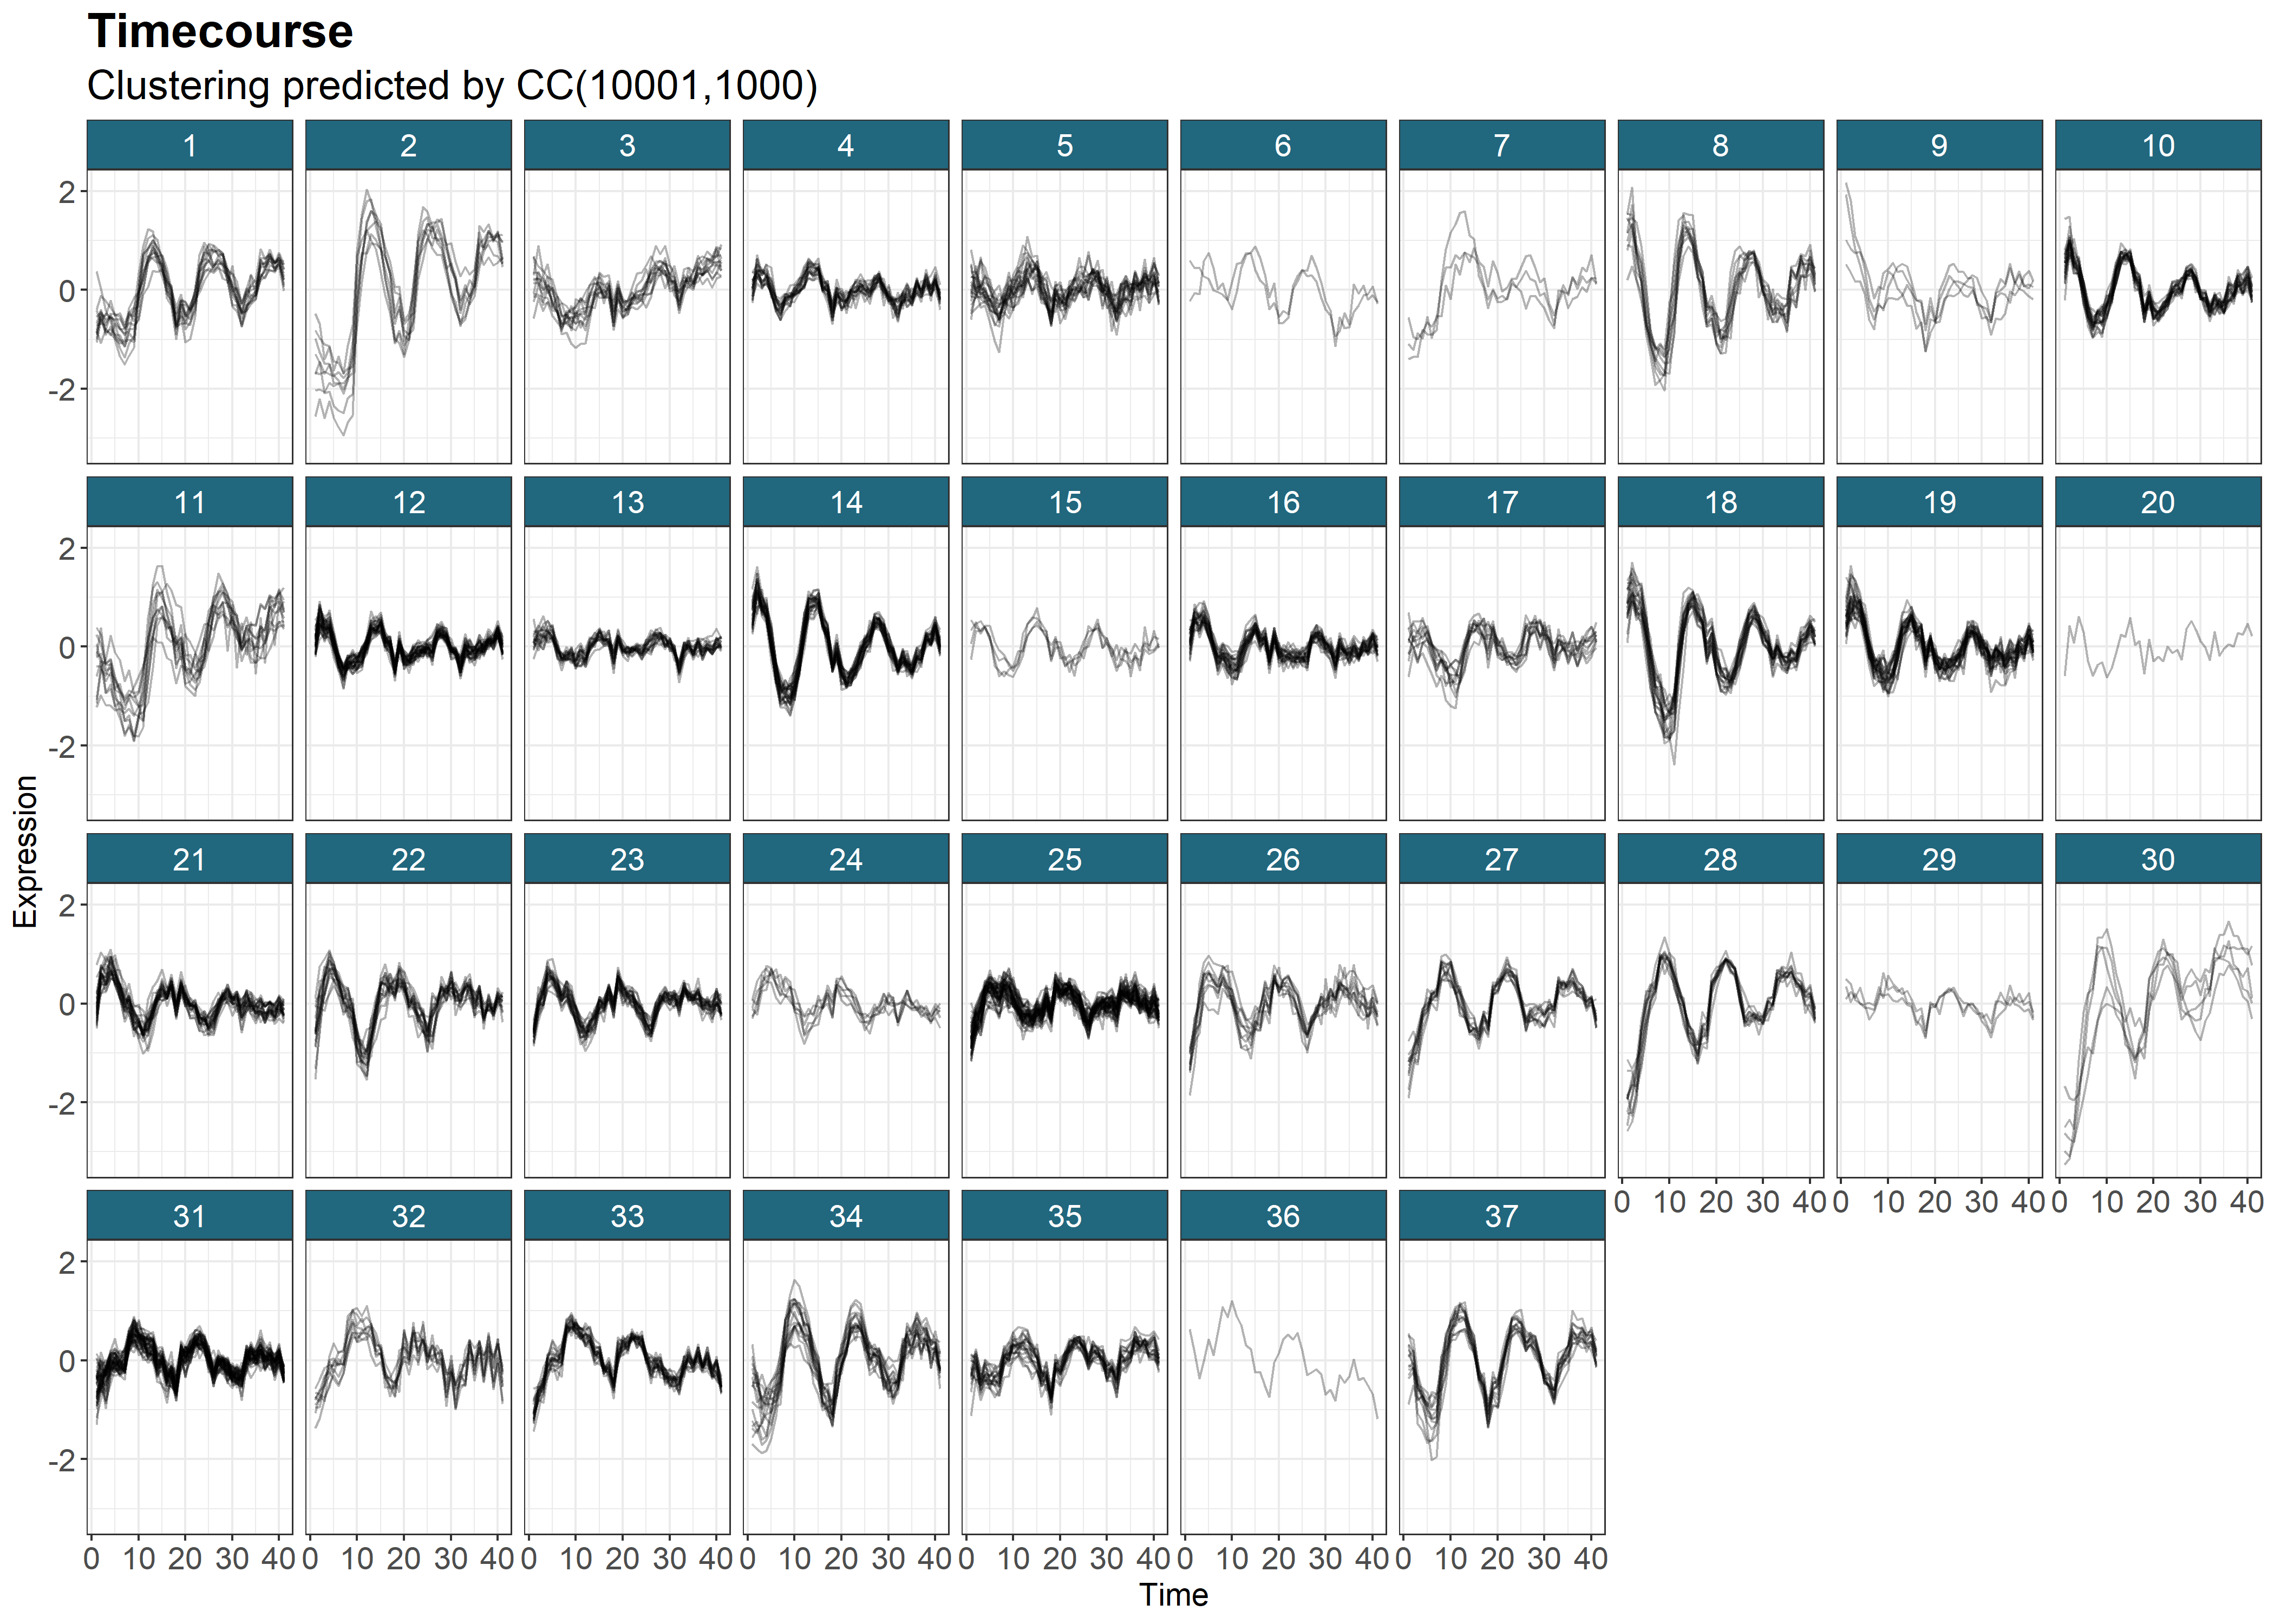
\includegraphics[scale=0.6]{./Images/Yeast/TimeSeriesClusterR10001S1000.png}
%	\caption{Gene expression across time for the predicted clusters in the Timecourse dataset for Consensus clustering of MDI with $R=10001$ and $S=1000$.}
%	\label{fig:timecourseCCTimeSeries}
%\end{sidewaysfigure}
%
%We also find that the clusters of time series in the Timecourse dataset shown in figure \ref{fig:timecourseCCTimeSeries} to be consistent.

\subsubsection{Timecourse - ChIP-chip fused}
Cluster 16 is nice! Histone proteins and then three others, GAS3, NRM1 and PDS1.

GAS3 is a poorly understood gene. We find that it is associated with HEK2 and SMT3 in the PPI data and SWI6, FKH2 and FKH1 in the ChIP-chip data. 

\begin{itemize}
	\item FKH1: Fkh1p cooperates with Isw1p to remodel chromatin during G2/M. FKH1 has additional roles in the establishment of chromatin silencing at the silent mating-type cassette and in the regulation of donor preference during mating type switching. FKH1 and the Swi4p/Swi6p-containing SCB-binding factor (SBF) independently regulate donor preference through direct interactions with a cis-acting sequence called the recombination enhancer, with Fkh1p binding in the G2 phase and SBF binding in the G1 phase of the cell cycle. 
	\item FKH2: negative role in chromatin silencing at HML and HMR.
	\item SWI6: Transcription cofactor. FKH1 and the Swi6p-containing SCB-binding factor (SBF) independently regulate donor preference through direct interactions with a cis-acting sequence called the recombination enhancer, with Fkh1p binding in the G2 phase and SBF binding in the G1 phase of the cell cycle.
	\item HEK2: RNA binding protein involved in asymmetric localization of ASH1 mRNA; represses translation of ASH1 mRNA, an effect reversed by Yck1p-dependent phosphoryation; regulates telomere position effect and length; similarity to hnRNP-K.
	\item SMT3: regulates chromatid cohesion, chromosome segregation, APC-mediated proteolysis, DNA replication and septin ring dynamics.
\end{itemize}
This suggests that GAS3 might be assoicated with chromosome/chormatin stuff. Not sure what this ``donor preference" stuff is, but it might be important for this.

NRM1: Transcriptional co-repressor of MBF-regulated gene expression; Nrm1p associates stably with promoters via MCB binding factor (MBF) to repress transcription upon exit from G1 phase. Approximately half of the members of cluster 16 have an interaction with MBF in the ChIP-chip data.

ESP1: An ESP1/PDS1 complex regulates loss of sister chromatid cohesion at the metaphase to anaphase transition in yeast \citep{ciosk1998esp1}.

Cluster 26 is also very consistent - 3 MCM complex genes and 2 others. Try to make a story.

	\begin{longtable}{@{\extracolsep{3pt}} cccp{85mm}} 
	\\[-1.8ex]\hline 
	\hline \\[-1.8ex] 
Gene & Name & Cluster & Description \\ 
\hline \\[-1.8ex] 
YNL078W & NIS1 & 1 & Protein localized in the bud neck at G2/M phase; physically interacts with septins; possibly involved in a mitotic signaling network \\ 
YIL009W & FAA3 & 1 & Long chain fatty acyl-CoA synthetase; activates imported fatty acids with a preference for C16:0-C18:0 chain lengths; green fluorescent protein (GFP)-fusion protein localizes to the cell periphery \\ 
YNL328C & MDJ2 & 1 & Constituent of the mitochondrial import motor; associated with the presequence translocase; function overlaps with that of Pam18p; stimulates the ATPase activity of Ssc1p to drive mitochondrial import; contains a J domain \\ \hline \\ [-1.8ex] 
YKL164C & PIR1 & 2 & O-glycosylated protein required for cell wall stability; attached to the cell wall via beta-1,3-glucan; mediates mitochondrial translocation of Apn1p; expression regulated by the cell integrity pathway and by Swi5p during the cell cycle; PIR1 has a paralog, YJL160C, that arose from the whole genome duplication \\ 
YNL327W & EGT2 & 2 & Glycosylphosphatidylinositol (GPI)-anchored cell wall endoglucanase; required for proper cell separation after cytokinesis; expression is activated by Swi5p and tightly regulated in a cell cycle-dependent manner \\ 
YKL185W & ASH1 & 2 & Component of the Rpd3L histone deacetylase complex; zinc-finger inhibitor of HO transcription; mRNA is localized and translated in the distal tip of anaphase cells, resulting in accumulation of Ash1p in daughter cell nuclei and inhibition of HO expression; potential Cdc28p substrate \\ 
YPL158C & AIM44 & 2 & Protein that regulates Cdc42p and Rho1p; functions in the late steps of cytokinesis and cell separation; sustains Rho1p at the cell division site after actomyosin ring contraction; inhibits the activation of Cdc42-Cla4 at the cell division site to prevent budding inside the old bud neck; transcription is regulated by Swi5p; null mutant displays elevated frequency of mitochondrial genome loss; relocalizes from bud neck to cytoplasm upon DNA replication stress \\ 
YDL179W & PCL9 & 2 & Cyclin; forms a functional kinase complex with Pho85p cyclin-dependent kinase (Cdk), expressed in late M/early G1 phase, activated by Swi5p; PCL9 has a paralog, PCL2, that arose from the whole genome duplication \\ \hline \\ [-1.8ex] 
YOR374W & ALD4 & 3 & Mitochondrial aldehyde dehydrogenase; required for growth on ethanol and conversion of acetaldehyde to acetate; phosphorylated; activity is K+ dependent; utilizes NADP+ or NAD+ equally as coenzymes; expression is glucose repressed; can substitute for cytosolic NADP-dependent aldehyde dehydrogenase when directed to the cytosol; human homolog ALDH2 can complement yeast ald4 mutant \\ 
YGL037C & PNC1 & 3 & Nicotinamidase that converts nicotinamide to nicotinic acid; part of the NAD(+) salvage pathway; required for life span extension by calorie restriction; lacks a peroxisomal targeting signal but is imported into peroxisomes via binding to Gpd1p; PNC1 expression responds to all known stimuli that extend replicative life span; protein increases in abundance and relative distribution to cytoplasmic foci decreases upon DNA replication stress \\ 
YCL040W & GLK1 & 3 & Glucokinase; catalyzes the phosphorylation of glucose at C6 in the first irreversible step of glucose metabolism; one of three glucose phosphorylating enzymes; expression regulated by non-fermentable carbon sources; GLK1 has a paralog, EMI2, that arose from the whole genome duplication \\ 
YFR053C & HXK1 & 3 & Hexokinase isoenzyme 1; a cytosolic protein that catalyzes phosphorylation of glucose during glucose metabolism; expression is highest during growth on non-glucose carbon sources; glucose-induced repression involves hexokinase Hxk2p; HXK1 has a paralog, HXK2, that arose from the whole genome duplication \\ \hline \\ [-1.8ex] 
YOR342C &  & 4 & Protein of unknown function; green fluorescent protein (GFP)-fusion protein localizes to the cytoplasm and the nucleus; relocalizes from nucleus to cytoplasm upon DNA replication stress; YOR342C has a paralog, YAL037W, that arose from the whole genome duplication \\ 
YGR289C & MAL11 & 4 & High-affinity maltose transporter (alpha-glucoside transporter); inducible; encoded in the MAL1 complex locus; broad substrate specificity that includes maltotriose; required for isomaltose utilization \\ 
YDL102W & POL3 & 4 & Catalytic subunit of DNA polymerase delta; required for chromosomal DNA replication during mitosis and meiosis, intragenic recombination, repair of double strand DNA breaks, and DNA replication during nucleotide excision repair (NER) \\ 
YLR457C & NBP1 & 4 & Spindle pole body (SPB) component; required for the insertion of the duplication plaque into the nuclear membrane during SPB duplication; essential for bipolar spindle formation; component of the Mps2p-Bbp1p complex; NBP1 has a paralog, YPR174C, that arose from the whole genome duplication \\ 
YBL010C &  & 4 & Putative protein of unknown function; green fluorescent protein (GFP)-fusion protein colocalizes with clathrin-coated vesicles \\ 
YBR098W & MMS4 & 4 & Subunit of structure-specific Mms4p-Mus81p endonuclease; cleaves branched DNA; involved in recombination, DNA repair, and joint molecule formation/resolution during meiotic recombination; phosphorylation of the non-catalytic subunit Mms4p by Cdc28p and Cdc5p during mitotic cell cycle activates the function of Mms4p-Mus81p \\ 
YDR440W & DOT1 & 4 & Nucleosomal histone H3-Lys79 methylase; methylation is required for telomeric silencing, meiotic checkpoint control, and DNA damage response \\ 
YHR127W &  & 4 & Protein of unknown function; localizes to the nucleus; required for asymmetric localization of Kar9p during mitosis \\ 
YGR042W & MTE1 & 4 & Protein of unknown function; involved in maintenance of proper telomere length; green fluorescent protein (GFP)-fusion protein localizes to both the cytoplasm and the nucleus; forms nuclear foci upon DNA replication stress \\ \hline \\ [-1.8ex] 
YER111C & SWI4 & 5 & DNA binding component of the SBF complex (Swi4p-Swi6p); a transcriptional activator that in concert with MBF (Mbp1-Swi6p) regulates late G1-specific transcription of targets including cyclins and genes required for DNA synthesis and repair; Slt2p-independent regulator of cold growth; acetylation at two sites, K1016 and K1066, regulates interaction with Swi6p \\ 
YKR077W & MSA2 & 5 & Putative transcriptional activator; interacts with G1-specific transcription factor MBF and G1-specific promoters; MSA2 has a paralog, MSA1, that arose from the whole genome duplication \\ 
YPL014W & CIP1 & 5 & Cyclin-dependent kinase inhibitor; interacts with and inhibits the Cdc28p/Cln2p, G1/S phase cyclin-dependent kinase complex but not S-phase, or M-phase complexes; overexpression blocks cells in G1 phase and stabilizes the Cdc28p inhibitor Sic1p, while disruption accelerates the G1/S phase transition; phosphorylated during S phase in a Cdc28p-dependent manner; green fluorescent protein (GFP)-fusion protein localizes to the cytoplasm and to the nucleus \\ 
YMR179W & SPT21 & 5 & Protein with a role in transcriptional silencing; required for normal transcription at several loci including HTA2-HTB2 and HHF2-HHT2, but not required at the other histone loci; functionally related to Spt10p; localizes to nuclear foci that become diffuse upon DNA replication stress \\ 
YGR109C & CLB6 & 5 & B-type cyclin involved in DNA replication during S phase; activates Cdc28p to promote initiation of DNA synthesis; functions in formation of mitotic spindles along with Clb3p and Clb4p; most abundant during late G1; CLB6 has a paralog, CLB5, that arose from the whole genome duplication \\ 
YPL267W & ACM1 & 5 & Pseudosubstrate inhibitor of the APC/C; suppresses APC/C [Cdh1]-mediated proteolysis of mitotic cyclins; associates with Cdh1p, Bmh1p and Bmh2p; cell cycle regulated protein; the anaphase-promoting complex/cyclosome is also known as APC/C \\ \hline \\ [-1.8ex] 
YDL156W & CMR1 & 6 & Nuclear protein with a role in protein quality control; localizes to the intranuclear quality control compartment (INQ) in response to proteasome inhibition or DNA replication stress; INQ likely sequesters proteins involved in DNA metabolism for degradation or re-folding; DNA-binding protein with preference for UV-damaged DNA; contains three WD domains (WD-40 repeat); human ortholog WDR76 also exhibits perinuclear localization under similar stress conditions \\ 
YFR027W & ECO1 & 6 & Acetyltransferase; required for establishment of sister chromatid cohesion; acetylates Mps3p to regulate nuclear organization; modifies Smc3p at replication forks and Mcd1p in response to dsDNA breaks; phosphorylated by three kinases (Cdc28p, Cdc7p, Mck1p) to generate pair of phosphates spaced precisely for recognition by ubiquitin ligase SCF-Cdc4; mutations in human homolog ESCO2 cause Roberts syndrome; relative distribution to nucleus increases upon DNA replication stress \\ 
YKL108W & SLD2 & 6 & Single-stranded DNA origin-binding and annealing protein; required for initiation of DNA replication; phosphorylated in S phase by cyclin-dependent kinases (Cdks), promoting origin binding, DNA replication and Dpb11p complex formation; component of the preloading complex; binds the Mcm2-7p complex to prevent inappropriate Mcm2-7p interaction with the GINS complex in G1; required for S phase checkpoint; relative distribution to the nucleus increases upon DNA replication stress \\ 
YNL309W & STB1 & 6 & Protein with role in regulation of MBF-specific transcription at Start; phosphorylated by Cln-Cdc28p kinases in vitro; unphosphorylated form binds Swi6p, which is required for Stb1p function; expression is cell-cycle regulated; STB1 has a paralog, YOL131W, that arose from the whole genome duplication \\ 
YOR144C & ELG1 & 6 & Subunit of an alternative replication factor C complex; important for DNA replication and genome integrity; suppresses spontaneous DNA damage; involved in homologous recombination-mediated repair and telomere homeostasis; required for PCNA (Pol30p) unloading during DNA replication \\ 
YJL181W & RBH1 & 6 & Putative protein of unknown function; expression is cell-cycle regulated as shown by microarray analysis; potential regulatory target of Mbp1p, which binds to the YJL181W promoter region; contains a PH-like domain; RBH1 has a paralog, RBH2, that arose from the whole genome duplication \\ 
YLR032W & RAD5 & 6 & DNA helicase/Ubiquitin ligase; involved in error-free DNA damage tolerance (DDT), replication fork regression during postreplication repair by template switching, error-prone translesion synthesis; promotes synthesis of free and PCNA-bound polyubiquitin chains by Ubc13p-Mms2p; forms nuclear foci upon DNA replication stress; associates with native telomeres, cooperates with homologous recombination in senescent cells; human homolog HLTF can complement yeast null mutant \\ 
YOR033C & EXO1 & 6 & 5'-3' exonuclease and flap-endonuclease; involved in recombination, double-strand break repair, MMS2 error-free branch of the post replication (PRR) pathway and DNA mismatch repair; role in telomere maintenance; member of the Rad2p nuclease family, with conserved N and I nuclease domains; relative distribution to the nucleus increases upon DNA replication stress; EXO1 has a paralog, DIN7, that arose from the whole genome duplication \\ 
YNL233W & BNI4 & 6 & Targeting subunit for Glc7p protein phosphatase; localized to the bud neck, required for localization of chitin synthase III to the bud neck via interaction with the chitin synthase III regulatory subunit Skt5p; phosphorylation by Slt2p and Kss1p involved in regulating Bni4p in septum assembly \\ 
YNL262W & POL2 & 6 & Catalytic subunit of DNA polymerase (II) epsilon; a chromosomal DNA replication polymerase that exhibits processivity and proofreading exonuclease activity; participates in leading-strand synthesis during DNA replication; also involved in DNA synthesis during DNA repair; interacts extensively with Mrc1p \\ 
YFL008W & SMC1 & 6 & Subunit of the multiprotein cohesin complex; essential protein involved in chromosome segregation and in double-strand DNA break repair; SMC chromosomal ATPase family member, binds DNA with a preference for DNA with secondary structure \\ \hline \\ [-1.8ex] 
YNL310C & ZIM17 & 7 & Protein co-chaperone with a zinc finger motif; essential for protein import into mitochondria; may act with Pam18p to facilitate recognition and folding of imported proteins by Ssc1p (mtHSP70) in the mitochondrial matrix; required for the maintenance of Ssc1p solubility and assists in the functional interaction of Ssc1p with substrate proteins \\ 
YDL103C & QRI1 & 7 & UDP-N-acetylglucosamine pyrophosphorylase; catalyzes the formation of UDP-N-acetylglucosamine (UDP-GlcNAc), which is important in cell wall biosynthesis, protein N-glycosylation, and GPI anchor biosynthesis; protein abundance increases in response to DNA replication stress \\ 
YLR233C & EST1 & 7 & TLC1 RNA-associated factor involved in telomere length regulation; recruitment subunit of telomerase; has G-quadruplex promoting activity required for telomere elongation; role in activating telomere-bound Est2p-TLC1-RNA; EST1 has a paralog, EBS1, that arose from the whole genome duplication \\ 
YLR382C & NAM2 & 7 & Mitochondrial leucyl-tRNA synthetase; also has direct role in splicing of several mitochondrial group I introns; indirectly required for mitochondrial genome maintenance; human homolog LARS2 can complement yeast null mutant, and is implicated in Perrault syndrome \\ 
YML020W &  & 7 & Putative protein of unknown function \\ 
YNL304W & YPT11 & 7 & Rab GTPase; Myo2p-binding protein implicated in mother-to-bud transport of cortical endoplasmic reticulum (ER), late Golgi, and mitochondria during cell division; function is regulated at multiple levels; abundance of active Ypt11p forms is controlled by phosphorylation status and degradation; normally a low-abundance protein whose ER localization is only detected when protein is highly over expressed \\ 
YAR003W & SWD1 & 7 & Subunit of the COMPASS (Set1C) complex; COMPASS methylates histone H3 on lysine 4 and is required in transcriptional silencing near telomeres; WD40 beta propeller superfamily member with similarity to mammalian Rbbp7 \\ 
YDR481C & PHO8 & 7 & Repressible vacuolar alkaline phosphatase; regulated by levels of Pi and by Pho4p, Pho9p, Pho80p, Pho81p and Pho85p; dephosphorylates phosphotyrosyl peptides; contributes to NAD+ metabolism by producing nicotinamide riboside from NMN \\ 
YHR159W & TDA11 & 7 & Putative protein of unknown function; green fluorescent protein (GFP)-fusion protein localizes to the cytoplasm; potential Cdc28p substrate; null mutant is sensitive to expression of the top1-T722A allele \\ 
YJR154W &  & 7 & Putative protein of unknown function; green fluorescent protein (GFP)-fusion protein localizes to the cytoplasm \\ 
YJR155W & AAD10 & 7 & Putative aryl-alcohol dehydrogenase; similar to P. chrysosporium aryl-alcohol dehydrogenase; mutational analysis has not yet revealed a physiological role; members of the AAD gene family comprise three pairs (AAD3 + AAD15, AAD6/AAD16 + AAD4, AAD10 + AAD14) whose two genes are more related to one another than to other members of the family \\ 
YLL002W & RTT109 & 7 & Histone acetyltransferase; critical for cell survival in presence of DNA damage during S phase, required for recovery after DSB repair; acetylates H3K56, H3K9; H3K56 acetylation activity required for expression homeostasis, buffering of mRNA synthesis rate against changes in gene dosage during S phase; involved in non-homologous end joining and regulation of Ty1 transposition; prevents hyper-amplification of rDNA; interacts physically with Vps75p \\ 
YLR212C & TUB4 & 7 & Gamma-tubulin; involved in nucleating microtubules from both the cytoplasmic and nuclear faces of the spindle pole body; protein abundance increases in response to DNA replication stress \\ 
YBR073W & RDH54 & 7 & DNA-dependent ATPase; DNA recombination/repair translocase, supercoils DNA and promotes DNA strand opening; stimulates strand exchange by modifying dsDNA topology; involved in recombinational repair of DNA double-strand breaks (DSBs) during mitosis and meiosis; phosphorylated in Mec1p-, Rad53p-dependent way in response to one DSB; contributes to remodelling of nucleosomes; proposed to be involved in crossover interference; interacts with Dmc1p; stimulates Dmc1p and Rad51p \\ 
YER170W & ADK2 & 7 & Mitochondrial adenylate kinase; catalyzes the reversible synthesis of GTP and AMP from GDP and ADP; may serve as a back-up for synthesizing GTP or ADP depending on metabolic conditions; 3' sequence of ADK2 varies with strain background \\ 
YOR288C & MPD1 & 7 & Member of the protein disulfide isomerase (PDI) family; interacts with and inhibits the chaperone activity of Cne1p; MPD1 overexpression in a pdi1 null mutant suppresses defects in Pdi1p functions such as carboxypeptidase Y maturation \\ 
YEL064C & AVT2 & 7 & Putative transporter; member of a family of seven S. cerevisiae genes (AVT1-7) related to vesicular GABA-glycine transporters \\ 
YBR275C & RIF1 & 7 & Protein that binds to the Rap1p C-terminus; acts synergistically with Rif2p to help control telomere length and establish telomeric silencing; involved in control of DNA replication; contributes to resection of DNA double strand breaks (DSBs); deletion results in telomere elongation \\ 
YJL019W & MPS3 & 7 & Nuclear envelope protein; required for SPB insertion, SPB duplication, Kar5p localization near the SPB and nuclear fusion; interacts with Mps2p to tether half-bridge to core SPB; N-terminal acetylation by Eco1p regulates its role in nuclear organization; localizes to the SPB half bridge and telomeres during meiosis; required with Ndj1p and Csm4p for meiotic bouquet formation and telomere-led rapid prophase movement; member of the SUN protein family (Sad1-UNC-84 homology) \\ 
YPL208W & RKM1 & 7 & SET-domain lysine-N-methyltransferase; catalyzes the formation of dimethyllysine residues on the large ribosomal subunit proteins L23 (Rpl23Ap and Rpl23Bp) and monomethyllysine residues on L18 (Rps18Ap and Rps18Bp) \\ 
YBR042C & CST26 & 7 & Acyltransferase; enzyme mainly responsible for the introduction of saturated very long chain fatty acids into neo-synthesized molecules of phosphatidylinositol; required for incorporation of stearic acid into phosphatidylinositol; affects chromosome stability when overexpressed; CST26 has a paralog, YDR018C, that arose from the whole genome duplication \\ 
YOR176W & HEM15 & 7 & Ferrochelatase; a mitochondrial inner membrane protein, catalyzes insertion of ferrous iron into protoporphyrin IX, the eighth and final step in the heme biosynthetic pathway; human homolog FECH can complement yeast mutant and allow growth of haploid null after sporulation of a heterozygous diploid \\ 
YKL092C & BUD2 & 7 & GTPase activating factor for Rsr1p/Bud1p; plays a role in spindle position checkpoint distinct from its role in bud site selection; required for both axial and bipolar budding patterns; mutants exhibit random budding in all cell types; contains two PH-like domains \\ \hline \\ [-1.8ex] 
YFL054C & AQY3 & 8 & Putative channel-like protein; similar to Fps1p; mediates passive diffusion of glycerol in the presence of ethanol \\ 
YDR517W & GRH1 & 8 & Acetylated cis-Golgi protein, involved in ER to Golgi transport; homolog of human GRASP65; forms a complex with the coiled-coil protein Bug1p; mutants are compromised for the fusion of ER-derived vesicles with Golgi membranes; protein abundance increases in response to DNA replication stress \\ 
YHR188C & GPI16 & 8 & Subunit of the glycosylphosphatidylinositol transamidase complex; transmembrane protein; adds GPIs to newly synthesized proteins; human PIG-Tp homolog \\ 
YDR348C & PAL1 & 8 & Protein of unknown function thought to be involved in endocytosis; physically interacts with Ede1p and is found at endocytic sites at cell periphery during early stages of endocytosis; green fluorescent protein (GFP)-fusion protein localizes to bud neck; potential Cdc28p substrate; similar to S. pombe Pal1 protein; relocalizes from bud neck to cytoplasm upon DNA replication stress; PAL1 has a paralog, YHR097C, that arose from the whole genome duplication \\ 
YER104W & RTT105 & 8 & Protein with a role in regulation of Ty1 transposition \\ 
YDL095W & PMT1 & 8 & Protein O-mannosyltransferase of the ER membrane; transfers mannose from dolichyl phosphate-D-mannose to protein serine and threonine residues; 1 of 7 related proteins involved in O-glycosylation which is essential for cell wall rigidity; involved in ER quality control; amino terminus faces cytoplasm, carboxyl terminus faces ER lumen \\ 
YAL007C & ERP2 & 8 & Member of the p24 family involved in ER to Golgi transport; similar to Emp24p and Erv25p; role in misfolded protein quality control; forms a heterotrimeric complex with Erp1p, Emp24p, and Erv25p; localized to COPII-coated vesicles; ERP2 has a paralog, ERP4, that arose from the whole genome duplication \\ \hline \\ [-1.8ex] 
YBL035C & POL12 & 9 & B subunit of DNA polymerase alpha-primase complex; required for initiation of DNA replication during mitotic and premeiotic DNA synthesis; also functions in telomere capping and length regulation \\ 
YNL273W & TOF1 & 9 & Subunit of a replication-pausing checkpoint complex; Tof1p-Mrc1p-Csm3p acts at the stalled replication fork to promote sister chromatid cohesion after DNA damage, facilitating gap repair of damaged DNA; interacts with the MCM helicase; relocalizes to the cytosol in response to hypoxia \\ 
YPR175W & DPB2 & 9 & Second largest subunit of DNA polymerase II (DNA polymerase epsilon); required for maintenance of fidelity of chromosomal replication; essential motif in C-terminus is required for formation of the four-subunit Pol epsilon; expression peaks at the G1/S phase boundary; Cdc28p substrate \\ 
YAR008W & SEN34 & 9 & Subunit of the tRNA splicing endonuclease; tRNA splicing endonuclease (Sen complex) is composed of Sen2p, Sen15p, Sen34p, and Sen54p; Sen complex also cleaves the CBP1 mRNA at the mitochondrial surface; Sen34p contains the active site for tRNA 3' splice site cleavage and has similarity to Sen2p and to Archaeal tRNA splicing endonuclease \\ 
YJL074C & SMC3 & 9 & Subunit of the multiprotein cohesin complex; required for sister chromatid cohesion in mitotic cells; also required, with Rec8p, for cohesion and recombination during meiosis; phylogenetically conserved SMC chromosomal ATPase family member \\ 
YDR097C & MSH6 & 9 & Protein required for mismatch repair in mitosis and meiosis; forms a complex with Msh2p to repair both single-base and insertion-deletion mispairs; also involved in interstrand cross-link repair; potentially phosphorylated by Cdc28p \\ 
YJL115W & ASF1 & 9 & Nucleosome assembly factor; involved in chromatin assembly, disassembly; required for recovery after DSB repair; role in H3K56 acetylation required for expression homeostasis, buffering mRNA synthesis rate against gene dosage changes in S phase; anti-silencing protein, derepresses silent loci when overexpressed; role in regulating Ty1 transposition; relocalizes to cytosol under hypoxia; growth defect of asf1 null is functionally complemented by either human ASF1A or ASF1B \\ 
YAR007C & RFA1 & 9 & Subunit of heterotrimeric Replication Protein A (RPA); RPA is a highly conserved single-stranded DNA binding protein involved in DNA replication, repair, and recombination; RPA protects against inappropriate telomere recombination, and upon telomere uncapping, prevents cell proliferation by a checkpoint-independent pathway; role in DNA catenation/decatenation pathway of chromosome disentangling; relocalizes to the cytosol in response to hypoxia \\ 
YCL061C & MRC1 & 9 & S-phase checkpoint protein required for DNA replication; couples DNA helicase and polymerase; interacts with and stabilizes Pol2p at stalled replication forks during stress, where it forms a pausing complex with Tof1p and is phosphorylated by Mec1p; defines a novel S-phase checkpoint with Hog1p that coordinates DNA replication and transcription upon osmostress; protects uncapped telomeres; Dia2p-dependent degradation mediates checkpoint recovery; mammalian claspin homolog \\ 
YLR103C & CDC45 & 9 & DNA replication initiation factor; recruited to MCM pre-RC complexes at replication origins; promotes release of MCM from Mcm10p, recruits elongation machinery; binds tightly to ssDNA, which disrupts interaction with the MCM helicase and stalls it during replication stress; mutants in human homolog may cause velocardiofacial and DiGeorge syndromes \\ 
YNL102W & POL1 & 9 & Catalytic subunit of the DNA polymerase I alpha-primase complex; required for the initiation of DNA replication during mitotic DNA synthesis and premeiotic DNA synthesis \\ 
YPL153C & RAD53 & 9 & DNA damage response protein kinase; required for cell-cycle arrest, regulation of copper genes in response to DNA damage; phosphorylates nuclear pores to counteract gene gating, preventing aberrant transitions at forks approaching transcribed genes; activates downstream kinase Dun1p; differentially senses mtDNA depletion, mitochondrial ROS; relocalizes to cytosol under hypoxia; human homolog CHEK2 implicated in breast cancer can complement yeast null mutant \\ 
YKL113C & RAD27 & 9 & 5' to 3' exonuclease, 5' flap endonuclease; required for Okazaki fragment processing and maturation, for long-patch base-excision repair and large loop repair (LLR), ribonucleotide excision repair; member of the S. pombe RAD2/FEN1 family; relocalizes to the cytosol in response to hypoxia \\ 
YIL026C & IRR1 & 9 & Subunit of the cohesin complex; which is required for sister chromatid cohesion during mitosis and meiosis and interacts with centromeres and chromosome arms; relocalizes to the cytosol in response to hypoxia; essential for viability \\ 
YNL312W & RFA2 & 9 & Subunit of heterotrimeric Replication Protein A (RPA); RPA is a highly conserved single-stranded DNA binding protein involved in DNA replication, repair, and recombination; RPA protects against inappropriate telomere recombination, and upon telomere uncapping, prevents cell proliferation by a checkpoint-independent pathway; in concert with Sgs1p-Top2p-Rmi1p, stimulates DNA catenation/decatenation activity of Top3p; protein abundance increases in response to DNA replication s \\ 
YPL241C & CIN2 & 9 & GTPase-activating protein (GAP) for Cin4p; tubulin folding factor C involved in beta-tubulin (Tub2p) folding; mutants display increased chromosome loss and benomyl sensitivity; human homolog RP2 complements yeast null mutant \\ \hline \\ [-1.8ex] 
YLR120C & YPS1 & 10 & Aspartic protease; hyperglycosylated member of the yapsin family of proteases, attached to the plasma membrane via a glycosylphosphatidylinositol (GPI) anchor; involved in nutrient limitation-induced cleavage of the extracellular inhibitory domain of signaling mucin Msb2p, resulting in activation of the filamentous growth MAPK pathway; involved with other yapsins in the cell wall integrity response; role in KEX2-independent processing of the alpha factor precursor \\ 
YLR234W & TOP3 & 10 & DNA Topoisomerase III; conserved protein that functions in a complex with Sgs1p and Rmi1p to relax single-stranded negatively-supercoiled DNA preferentially; DNA catenation/decatenation activity is stimulated by RPA and Sgs1p-Top3p-Rmi1p; involved in telomere stability and regulation of mitotic recombination \\ 
YNL165W &  & 10 & Putative protein of unknown function; YNL165W is not an essential gene \\ 
YIL132C & CSM2 & 10 & Component of Shu complex (aka PCSS complex); Shu complex also includes Psy3, Shu1, Shu2, and promotes error-free DNA repair,; Shu complex mediates inhibition of Srs2p function; promotes formation of Rad51p filaments; Psy3p and Csm2p contain similar DNA-binding regions which work together to form a single DNA binding site; required for accurate chromosome segregation during meiosis \\ 
YKL089W & MIF2 & 10 & Protein required for structural integrity of elongating spindles; localizes to the kinetochore; interacts with histones H2A, H2B, and H4; phosphorylated by Ipl1p; orthologous to human centromere constitutive-associated network (CCAN) subunit CENP-C and fission yeast cnp3 \\ 
YKL165C & MCD4 & 10 & Protein involved in GPI anchor synthesis; multimembrane-spanning protein that localizes to the endoplasmic reticulum; highly conserved among eukaryotes; GPI stands for glycosylphosphatidylinositol \\ 
YDR518W & EUG1 & 10 & Protein disulfide isomerase of the endoplasmic reticulum lumen; EUG1 has a paralog, PDI1, that arose from the whole genome duplication; function overlaps with that of Pdi1p; may interact with nascent polypeptides in the ER \\ 
YGL027C & CWH41 & 10 & Processing alpha glucosidase I; ER type II integral membrane N-glycoprotein involved in assembly of cell wall beta 1,6 glucan and asparagine-linked protein glycosylation; also involved in ER protein quality control and sensing of ER stress \\ 
YML061C & PIF1 & 10 & DNA helicase, potent G-quadruplex DNA binder/unwinder; possesses strand annealing activity; promotes DNA synthesis during break-induced replication; important for crossover recombination; translation from different start sites produces mitochondrial and nuclear forms; nuclear form is a catalytic inhibitor of telomerase; mitochondrial form involved in DNA repair and recombination; mutations affect Zn, Fe homeostasis; regulated by Rad53p-dependent phosphorylation in rho0 cells \\ 
YDL093W & PMT5 & 10 & Protein O-mannosyltransferase; transfers mannose residues from dolichyl phosphate-D-mannose to protein serine/threonine residues; acts in a complex with Pmt3p, can instead interact with Pmt2p in some conditions; target for new antifungals \\ 
YGL175C & SAE2 & 10 & Endonuclease required for telomere elongation; required for telomeric 5' C-rich strand resection; involved in ds-break repair and processing hairpin DNA structures with the MRX complex; function requires sumoylation and phosphorylation; exists as inactive oligomers that are transiently released into smaller active units by phosphorylation; DNA damage triggers Sae2p removal, so active Sae2p is present only transiently; sequence and functional similarity with human CtIP/RBBP8 \\ 
YLR151C & PCD1 & 10 & 8-oxo-dGTP diphosphatase; prevents spontaneous mutagenesis via sanitization of oxidized purine nucleoside triphosphates; can also act as peroxisomal pyrophosphatase with specificity for coenzyme A and CoA derivatives, may function to remove potentially toxic oxidized CoA disulfide from peroxisomes to maintain the capacity for beta-oxidation of fatty acids; nudix hydrolase family member; similar E. coli MutT and human, rat and mouse MTH1 \\ 
YLR381W & CTF3 & 10 & Outer kinetochore protein that forms a complex with Mcm16p and Mcm22p; may bind the kinetochore to spindle microtubules; required for the spindle assembly checkpoint; orthologous to human centromere constitutive-associated network (CCAN) subunit CENP-I and fission yeast mis6 \\ 
YAL034W-A & MTW1 & 10 & Essential component of the MIND kinetochore complex; joins kinetochore subunits contacting DNA to those contacting microtubules; critical to kinetochore assembly; complex consists of Mtw1p Including Nnf1p-Nsl1p-Dsn1p (MIND) \\ 
YKL067W & YNK1 & 10 & Nucleoside diphosphate kinase; catalyzes the transfer of gamma phosphates from nucleoside triphosphates, usually ATP, to nucleoside diphosphates by a mechanism that involves formation of an autophosphorylated enzyme intermediate; protein abundance increases in response to DNA replication stress \\ 
YGL094C & PAN2 & 10 & Catalytic subunit of the Pan2p-Pan3p poly(A)-ribonuclease complex; complex acts to control poly(A) tail length and regulate the stoichiometry and activity of postreplication repair complexes \\ 
YOR081C & TGL5 & 10 & Bifunctional triacylglycerol lipase and LPA acyltransferase; lipid particle-localized triacylglycerol (TAG) lipase involved in triacylglycerol mobilization; catalyzes acylation of lysophosphatidic acid (LPA); potential Cdc28p substrate; TGL5 has a paralog, TGL4, that arose from the whole genome duplication \\ 
YFL025C & BST1 & 10 & GPI inositol deacylase of the endoplasmic reticulum (ER); negatively regulates COPII vesicle formation; prevents production of vesicles with defective subunits; required for proper discrimination between resident ER proteins and Golgi-bound cargo molecules; functional ortholog of human PGAP1, mutation of which is associated with intellectual disability and encephalopathy \\ \hline \\ [-1.8ex] 
YKR013W & PRY2 & 11 & Sterol binding protein involved in the export of acetylated sterols; secreted glycoprotein and member of the CAP protein superfamily (cysteine-rich secretory proteins (CRISP), antigen 5, and pathogenesis related 1 proteins); sterol export function is redundant with that of PRY1; may be involved in detoxification of hydrophobic compounds; PRY2 has a paralog, PRY1, that arose from the whole genome duplication \\ 
YPL163C & SVS1 & 11 & Cell wall and vacuolar protein; required for wild-type resistance to vanadate; SVS1 has a paralog, SRL1, that arose from the whole genome duplication \\ 
YGR014W & MSB2 & 11 & Mucin family member involved in various signaling pathways; functions as osmosensor in the Sho1p-mediated HOG pathway; functions in Cdc42p- and MAP kinase-dependent filamentous growth signaling pathway; processed into secreted and cell-associated forms by aspartyl protease Yps1p; potential Cdc28p substrate \\ \hline \\ [-1.8ex] 
YDL003W & MCD1 & 12 & Essential alpha-kleisin subunit of the cohesin complex; required for sister chromatid cohesion in mitosis and meiosis; apoptosis induces cleavage and translocation of a C-terminal fragment to mitochondria; expression peaks in S phase \\ 
YER070W & RNR1 & 12 & Major isoform of large subunit of ribonucleotide-diphosphate reductase; the RNR complex catalyzes rate-limiting step in dNTP synthesis, regulated by DNA replication and DNA damage checkpoint pathways via localization of small subunits; relative distribution to the nucleus increases upon DNA replication stress; RNR1 has a paralog, RNR3, that arose from the whole genome duplication \\ 
YGR221C & TOS2 & 12 & Protein involved in localization of Cdc24p to the site of bud growth; may act as a membrane anchor; localizes to the bud neck and bud tip; potentially phosphorylated by Cdc28p; TOS2 has a paralog, SKG6, that arose from the whole genome duplication \\ 
YML027W & YOX1 & 12 & Homeobox transcriptional repressor; binds to Mcm1p and to early cell cycle boxes (ECBs) in the promoters of cell cycle-regulated genes expressed in M/G1 phase; expression is cell cycle-regulated; phosphorylated by Cdc28p; relocalizes from nucleus to cytoplasm upon DNA replication stress; YOX1 has a paralog, YHP1, that arose from the whole genome duplication \\ 
YER095W & RAD51 & 12 & Strand exchange protein; forms a helical filament with DNA that searches for homology; involved in the recombinational repair of double-strand breaks in DNA during vegetative growth and meiosis; homolog of Dmc1p and bacterial RecA protein \\ 
YNL289W & PCL1 & 12 & Cyclin, interacts with cyclin-dependent kinase Pho85p; member of the Pcl1,2-like subfamily, involved in the regulation of polarized growth and morphogenesis and progression through the cell cycle; is ubiquitinated by Dma1p; phosphorylation by Pho85p targets it for degradation; localizes to sites of polarized cell growth \\ 
YOR074C & CDC21 & 12 & Thymidylate synthase; required for de novo biosynthesis of pyrimidine deoxyribonucleotides; expression is induced at G1/S; human homolog TYMSOS can complement yeast cdc21 temperature-sensitive mutant at restrictive temperature \\ 
YJL187C & SWE1 & 12 & Protein kinase that regulates the G2/M transition; negative regulator of the Cdc28p kinase; morphogenesis checkpoint kinase; positive regulator of sphingolipid biosynthesis via Orm2p; phosphorylates a tyrosine residue in the N-terminus of Hsp90 in a cell-cycle associated manner, thus modulating the ability of Hsp90 to chaperone a selected clientele; localizes to the nucleus and to the daughter side of the mother-bud neck; homolog of S. pombe Wee1p; potential Cdc28p substrate \\ 
YOL007C & CSI2 & 12 & Protein of unknown function; green fluorescent protein (GFP)- fusion protein localizes to the mother side of the bud neck and the vacuole; YOL007C is not an essential gene \\ \hline \\ [-1.8ex] 
YHR153C & SPO16 & 13 & Meiosis-specific protein involved in synaptonemal complex assembly; implicated in regulation of crossover formation; required for sporulation \\ 
YML060W & OGG1 & 13 & Nuclear and mitochondrial glycosylase/lyase; specifically excises 7,8-dihydro-8-oxoguanine residues located opposite cytosine or thymine residues in DNA, repairs oxidative damage to mitochondrial DNA, contributes to UVA resistance \\ 
YPL057C & SUR1 & 13 & Mannosylinositol phosphorylceramide (MIPC) synthase catalytic subunit; forms a complex with regulatory subunit Csg2p; function in sphingolipid biosynthesis is overlapping with that of Csh1p; SUR1 has a paralog, CSH1, that arose from the whole genome duplication \\ 
YDR400W & URH1 & 13 & Uridine nucleosidase (uridine-cytidine N-ribohydrolase); cleaves N-glycosidic bonds in nucleosides; involved in the pyrimidine salvage and nicotinamide riboside salvage pathways \\ 
YDR503C & LPP1 & 13 & Lipid phosphate phosphatase; catalyzes Mg(2+)-independent dephosphorylation of phosphatidic acid (PA), lysophosphatidic acid, and diacylglycerol pyrophosphate; involved in control of the cellular levels of phosphatidylinositol and PA \\ 
YNL072W & RNH201 & 13 & Ribonuclease H2 catalytic subunit; removes RNA primers during Okazaki fragment synthesis and errant ribonucleotides misincorporated during DNA replication; role in ribonucleotide excision repair; homolog of RNAse HI; related to human AGS4 which causes Aicardi-Goutieres syndrome \\ 
YOL019W &  & 13 & Protein of unknown function; green fluorescent protein (GFP)-fusion protein localizes to the cell periphery and vacuole; YOL019W has a paralog, DCV1, that arose from the whole genome duplication \\ 
YKL042W & SPC42 & 13 & Central plaque component of spindle pole body (SPB); involved in SPB duplication, may facilitate attachment of the SPB to the nuclear membrane \\ 
YDL010W & GRX6 & 13 & Cis-golgi localized monothiol glutaredoxin, binds Fe-S cluster; more similar in activity to dithiol than other monothiol glutaredoxins; involved in the oxidative stress response; GRX6 has a paralog, GRX7, that arose from the whole genome duplication \\ 
YDL197C & ASF2 & 13 & Anti-silencing protein; causes derepression of silent loci when overexpressed \\ 
YDL211C &  & 13 & Protein of unknown function; green fluorescent protein (GFP)-fusion protein localizes to the vacuole; YDL211C has a paralog, TDA7, that arose from the whole genome duplication \\ 
YOR114W &  & 13 & Putative protein of unknown function; null mutant is viable \\ 
YOR321W & PMT3 & 13 & Protein O-mannosyltransferase; transfers mannose residues from dolichyl phosphate-D-mannose to protein serine/threonine residues; acts in a complex with Pmt5p, can instead interact with Pmt1p in some conditions; antifungal drug target; PMT3 has a paralog, PMT2, that arose from the whole genome duplication \\ 
YHR110W & ERP5 & 13 & Protein with similarity to Emp24p and Erv25p; member of the p24 family involved in ER to Golgi transport \\ 
YLR383W & SMC6 & 13 & Component of the SMC5-SMC6 complex; this complex plays a key role in the removal of X-shaped DNA structures that arise between sister chromatids during DNA replication and repair; homologous to S. pombe rad18 \\ 
YDR501W & PLM2 & 13 & Putative transcription factor, contains Forkhead Associated domain; found associated with chromatin; target of SBF transcription factor; induced in response to DNA damaging agents and deletion of telomerase; PLM2 has a paralog, TOS4, that arose from the whole genome duplication \\ 
YLR050C &  & 13 & Putative protein of unknown function; green fluorescent protein (GFP)-fusion protein localizes to the endoplasmic reticulum; YLR050C is not an essential gene \\ \hline \\ [-1.8ex] 
YJL091C & GWT1 & 14 & Protein involved in the inositol acylation of GlcN-PI; the inositol acylation of glucosaminyl phosphatidylinositol (GlcN-PI) forms glucosaminyl(acyl)phosphatidylinositol (GlcN(acyl)PI), an intermediate in the biosynthesis of glycosylphosphatidylinositol (GPI) anchors \\ \hline \\ [-1.8ex] 
YOR195W & SLK19 & 15 & Kinetochore-associated protein; required for chromosome segregation and kinetochore clustering; required for normal segregation of chromosomes in meiosis and mitosis; component of the FEAR regulatory network, which promotes Cdc14p release from the nucleolus during anaphase; potential Cdc28p substrate \\ 
YDR480W & DIG2 & 15 & MAP kinase-responsive inhibitor of the Ste12p transcription factor; involved in the regulation of mating-specific genes and the invasive growth pathway; related regulators Dig1p and Dig2p bind to Ste12p; DIG2 has a paralog, DIG1, that arose from the whole genome duplication \\ 
YDR488C & PAC11 & 15 & Dynein intermediate chain, microtubule motor protein; required for intracellular transport and cell division; acts in cytoplasmic dynein pathway; forms complex with dynein light chain Dyn2p that promotes Dyn1p homodimerization and potentiates motor processivity; Dyn2p-Pac11p complex is also important for interaction of dynein motor complex with dynactin complex; forms cortical cytoplasmic microtubule capture site with Num1p; essential in the absence of CIN8 \\ 
YGR188C & BUB1 & 15 & Protein kinase involved in the cell cycle checkpoint into anaphase; in complex with Mad1p and Bub3p, prevents progression into anaphase in presence of spindle damage; Cdc28p-mediated phosphorylation at Bub1p-T566 is important for degradation in anaphase and adaptation of checkpoint to prolonged mitotic arrest; associates with centromere DNA via Skp1p; involved in Sgo1p relocalization in response to sister kinetochore tension; paralog MAD3 arose from whole genome duplication \\ 
YER003C & PMI40 & 15 & Mannose-6-phosphate isomerase; catalyzes the interconversion of fructose-6-P and mannose-6-P; required for early steps in protein mannosylation \\ 
YGL093W & SPC105 & 15 & Subunit of a kinetochore-microtubule binding complex; complex bridges centromeric heterochromatin and kinetochore MAPs and motors; required for sister chromatid bi-orientation and kinetochore binding of SAC components; complex also includes Kre28p; modified by sumoylation \\ 
YMR144W & FDO1 & 15 & Protein involved in directionality of mating type switching; acts with Fkh1p to control which donor mating-type locus is inserted into MAT locus during mating type switching; localized to the nucleus; not an essential gene \\ 
YNL088W & TOP2 & 15 & Topoisomerase II; relieves torsional strain in DNA by cleaving and re-sealing phosphodiester backbone of both positively and negatively supercoiled DNA; cleaves complementary strands; localizes to axial cores in meiosis; required for replication slow zone (RSZ) breakage following Mec1p inactivation; human homolog TOP2A implicated in cancers, and can complement yeast null mutant \\ 
YOR083W & WHI5 & 15 & Repressor of G1 transcription; binds to SCB binding factor (SBF) at SCB target promoters in early G1; dilution of Whi5p concentration during cell growth determines cell size; phosphorylation of Whi5p by the CDK, Cln3p/Cdc28p relieves repression and promoter binding by Whi5, and contributes to both the determination of critical cell size at START and cell fate; periodically expressed in G1 \\ 
YDR356W & SPC110 & 15 & Inner plaque spindle pole body (SPB) component; ortholog of human kendrin; gamma-tubulin small complex (gamma-TuSC) receptor that interacts with Spc98p to recruit the complex to the nuclear side of the SPB, connecting nuclear microtubules to the SPB; promotes gamma-TuSC assembly and oligomerization to initiate microtubule nucleation; interacts with Tub4p-complex and calmodulin; phosphorylated by Mps1p in cell cycle-dependent manner \\ 
YLL021W & SPA2 & 15 & Component of the polarisome; functions in actin cytoskeletal organization during polarized growth; acts as a scaffold for Mkk1p and Mpk1p cell wall integrity signaling components; potential Cdc28p substrate; coding sequence contains length polymorphisms in different strains; SPA2 has a paralog, SPH1, that arose from the whole genome duplication \\ 
YBL009W & ALK2 & 15 & Protein kinase; along with its paralog, ALK1, required for proper spindle positioning and nuclear segregation following mitotic arrest, proper organization of cell polarity factors in mitosis, proper localization of formins and polarity factors, and survival in cells that activate spindle assembly checkpoint; phosphorylated in response to DNA damage; ALK2 has a paralog, ALK1, that arose from the whole genome duplication; similar to mammalian haspins \\ 
YHR172W & SPC97 & 15 & Component of the microtubule-nucleating Tub4p (gamma-tubulin) complex; interacts with Spc110p at the spindle pole body (SPB) inner plaque and with Spc72p at the SPB outer plaque \\ 
YNL166C & BNI5 & 15 & Linker protein responsible for recruitment of myosin to the bud neck; interacts with the C-terminal extensions of septins Cdc11p and Shs1p and binds Myo1p to promote cytokinesis \\ 
YER019W & ISC1 & 15 & Inositol phosphosphingolipid phospholipase C; mitochondrial membrane localized; hydrolyzes complex sphingolipids to produce ceramide; activates genes required for non-fermentable carbon source metabolism during diauxic shift; activated by phosphatidylserine, cardiolipin, and phosphatidylglycerol; mediates Na+ and Li+ halotolerance; ortholog of mammalian neutral sphingomyelinase type 2 \\ 
YBL031W & SHE1 & 15 & Mitotic spindle protein; interacts with components of the Dam1 (DASH) complex, its effector Sli15p, and microtubule-associated protein Bim1p; also localizes to nuclear microtubules and to the bud neck in a ring-shaped structure; inhibits dynein function \\ 
YPR141C & KAR3 & 15 & Minus-end-directed microtubule motor; functions in mitosis and meiosis, localizes to the spindle pole body and localization is dependent on functional Cik1p, required for nuclear fusion during mating; potential Cdc28p substrate \\ \hline \\ [-1.8ex] 
YDR113C & PDS1 & 16 & Securin; inhibits anaphase by binding separin Esp1p; blocks cyclin destruction and mitotic exit, essential for meiotic progression and mitotic cell cycle arrest; localization is cell-cycle dependent and regulated by Cdc28p phosphorylation \\ 
YNL030W & HHF2 & 16 & 
%Histone H4; 
Core histone protein required for chromatin assembly and chromosome function
%; one of two identical histone proteins (see also HHF1); contributes to telomeric silencing; N-terminal domain involved in maintaining genomic integrity 
\\ 
YPL127C & HHO1 & 16 & Histone protein 
%Histone H1, linker histone with roles in meiosis and sporulation; decreasing levels early in sporulation may promote meiosis, and increasing levels during sporulation facilitate compaction of spore chromatin; binds to promoters and within genes in mature spores; may be recruited by Ume6p to promoter regions, contributing to transcriptional repression outside of meiosis; suppresses DNA repair involving homologous recombination 
\\ 
YBL002W & HTB2 & 16 & 
%Histone H2B; 
Core histone protein required for chromatin assembly and chromosome function
%; nearly identical to HTB1; Rad6p-Bre1p-Lge1p mediated ubiquitination regulates reassembly after DNA replication, transcriptional activation, meiotic DSB formation and H3 methylation 
\\ 
YDR225W & HTA1 & 16 & 
%Histone H2A; 
Core histone protein required for chromatin assembly and chromosome function
%; one of two nearly identical subtypes (see also HTA2); DNA damage-dependent phosphorylation by Mec1p facilitates DNA repair; acetylated by Nat4p; N-terminally propionylated in vivo 
\\ 
YBR010W & HHT1 & 16 & 
%Histone H3; 
Core histone protein required for chromatin assembly
%, part of heterochromatin-mediated telomeric and HM silencing; one of two identical histone H3 proteins (see HHT2); regulated by acetylation, methylation, and phosphorylation; H3K14 acetylation plays an important role in the unfolding of strongly positioned nucleosomes during repair of UV damage 
\\ 
YDR224C & HTB1 & 16 & 
%Histone H2B; 
Core histone protein required for chromatin assembly and chromosome function
%; nearly identical to HTB2; Rad6p-Bre1p-Lge1p mediated ubiquitination regulates reassembly after DNA replication, transcriptional activation, meiotic DSB formation and H3 methylation 
\\ 
YNL031C & HHT2 & 16 & 
%Histone H3; 
Core histone protein required for chromatin assembly 
%, part of heterochromatin-mediated telomeric and HM silencing; one of two identical histone H3 proteins (see HHT1); regulated by acetylation, methylation, and phosphorylation; H3K14 acetylation plays an important role in the unfolding of strongly positioned nucleosomes during repair of UV damage 
\\ 
YBL003C & HTA2 & 16 & 
%Histone H2A; 
Core histone protein required for chromatin assembly and chromosome function
%; one of two nearly identical (see also HTA1) subtypes; DNA damage-dependent phosphorylation by Mec1p facilitates DNA repair; acetylated by Nat4p 
\\ 
YNR009W & NRM1 & 16 & Transcriptional co-repressor of MBF-regulated gene expression; Nrm1p associates stably with promoters via MCB binding factor (MBF) to repress transcription upon exit from G1 phase \\ 
YBR009C & HHF1 & 16 & 
%Histone H4; 
Core histone protein required for chromatin assembly and chromosome function
%; one of two identical histone proteins (see also HHF2); contributes to telomeric silencing; N-terminal domain involved in maintaining genomic integrity 
\\ 
YMR215W & GAS3 & 16 & Putative 1,3-beta-glucanosyltransferase; has similarity go other GAS family members; low abundance, possibly inactive member of the GAS family of GPI-containing proteins; localizes to the cell wall; mRNA induced during sporulation \\ \hline \\ [-1.8ex] 
YMR117C & SPC24 & 17 & Component of the kinetochore-associated Ndc80 complex; involved in chromosome segregation, spindle checkpoint activity, and kinetochore clustering; evolutionarily conserved; other members include Ndc80p, Nuf2p, Spc24p, and Spc25p \\ 
YGR099W & TEL2 & 17 & Subunit of the ASTRA complex, involved in chromatin remodeling; subunit of the telomere cap complex DNA-binding protein specific to single-stranded yeast telomeric DNA repeats, required for telomere length regulation and telomere position effect; involved in the stability or biogenesis of PIKKs such as TORC1 \\ 
YPL116W & HOS3 & 17 & Trichostatin A-insensitive homodimeric histone deacetylase (HDAC); specificity in vitro for histones H3, H4, H2A, and H2B; similar to Hda1p, Rpd3p, Hos1p, and Hos2p; deletion results in increased histone acetylation at rDNA repeats \\ 
YLR210W & CLB4 & 17 & B-type cyclin involved in cell cycle progression; activates Cdc28p to promote the G2/M transition; may be involved in DNA replication and spindle assembly; accumulates during S phase and G2, then targeted for ubiquitin-mediated degradation; CLB4 has a paralog, CLB3, that arose from the whole genome duplication \\ 
YNL176C & TDA7 & 17 & Cell cycle-regulated gene of unknown function; promoter bound by Fkh2p; null mutant is sensitive to expression of the top1-T722A allele; TDA7 has a paralog, YDL211C, that arose from the whole genome duplication \\ \hline \\ [-1.8ex] 
YLR209C & PNP1 & 18 & Purine nucleoside phosphorylase; specifically metabolizes inosine and guanosine nucleosides; involved in the nicotinamide riboside salvage pathway \\ \hline \\ [-1.8ex] 
YMR006C & PLB2 & 19 & Phospholipase B (lysophospholipase) involved in lipid metabolism; displays transacylase activity in vitro; overproduction confers resistance to lysophosphatidylcholine \\ 
YGR113W & DAM1 & 19 & Essential subunit of the Dam1 complex (aka DASH complex); cooperates with Duo1p to connect the DASH complex with the microtubules (MT); couples kinetochores to the force produced by MT depolymerization thereby aiding in chromosome segregation; Ipl1p target for regulating kinetochore-MT attachments \\ 
YLR288C & MEC3 & 19 & DNA damage and meiotic pachytene checkpoint protein; subunit of a heterotrimeric complex (Rad17p-Mec3p-Ddc1p) that forms a sliding clamp, loaded onto partial duplex DNA by a clamp loader complex; homolog of human and S. pombe Hus1 \\ 
YIR010W & DSN1 & 19 & Essential component of the MIND kinetochore complex; joins kinetochore subunits contacting DNA to those contacting microtubules; Dsn1p phosphorylation promotes interaction between outer and inner kinetochore proteins; kinetochore receptor for monopolin, via interaction with subunit Csm1p; essential for meiotic but not mitotic chromosome segregation; MIND complex consists of Mtw1p, Nnf1p, Nsl1p and Dsn1p; modified by sumoylation; phosphorylated by monopolin subunit Hrr25p \\ 
YBL097W & BRN1 & 19 & Subunit of the condensin complex; required for chromosome condensation and for clustering of tRNA genes at the nucleolus; may influence multiple aspects of chromosome transmission \\ 
YGL101W &  & 19 & Protein of unknown function; non-essential gene; interacts with the DNA helicase Hpr5p; YGL101W has a paralog, YBR242W, that arose from the whole genome duplication \\ 
YJR076C & CDC11 & 19 & Component of the septin ring that is required for cytokinesis; present at the ends of rod-like septin hetero-oligomers; C-terminal extension is important for recruitment of Bni5p to the mother-bud neck, which in turn is required for Myo1p recruitment and cytokinesis; septin rings at the mother-bud neck act as scaffolds for recruiting cell division factors and as barriers to prevent diffusion of specific proteins between mother and daughter cells \\ 
YKL048C & ELM1 & 19 & Serine/threonine protein kinase; regulates the orientation checkpoint, the morphogenesis checkpoint and the metabolic switch from fermentative to oxidative metabolism by phosphorylating the activation loop of Kin4p, Hsl1p and Snf4p respectively; cooperates with Hsl7p in recruiting Hsl1p to the septin ring, a prerequisite for subsequent recruitment, phosphorylation, and degradation of Swe1p; forms part of the bud neck ring; regulates cytokinesis \\ 
YKL069W &  & 19 & Methionine-R-sulfoxide reductase; reduces the R enantiomer of free Met-SO, in contrast to Ycl033Cp which reduces Met-R-SO in a peptide linkage; has a role in protection against oxidative stress; relative distribution to the nucleus increases upon DNA replication stress \\ 
YMR190C & SGS1 & 19 & RecQ family nucleolar DNA helicase; role in genome integrity maintenance, chromosome synapsis, meiotic joint molecule/crossover formation; stimulates activity of Top3p; rapidly lost in response to rapamycin in Rrd1p-dependent manner; forms nuclear foci upon DNA replication stress; yeast SGS1 complements mutations in human homolog BLM implicated in Bloom syndrome; also similar to human WRN implicated in Werner syndrome; human BLM and WRN can each complement yeast null mutant \\ 
YDL028C & MPS1 & 19 & Dual-specificity kinase; autophosphorylation required for function; required for spindle pole body (SPB) duplication and spindle checkpoint function; contributes to bi-orientation by promoting formation of force-generating kinetochore-microtubule attachments in meiosis I; substrates include SPB proteins Spc42p, Spc110p, and Spc98p, mitotic exit network protein Mob1p, kinetochore protein Cnn1p, and checkpoint protein Mad1p; substrate of APCC(Cdh1); similar to human Mps1p \\ 
YDR130C & FIN1 & 19 & Spindle pole body-related intermediate filament protein; forms cell cycle-specific filaments between spindle pole bodies in dividing cells; localizes to poles and microtubules of spindle during anaphase and contributes to spindle stability; involved in Glc7p localization and regulation; relative distribution to the nucleus increases upon DNA replication stress \\ 
YDR227W & SIR4 & 19 & SIR protein involved in assembly of silent chromatin domains; silent information regulator (SIR) along with SIR2 and SIR3; involved in assembly of silent chromatin domains at telomeres and the silent mating-type loci; some alleles of SIR4 prolong lifespan; required for telomere hypercluster formation in quiescent yeast cells \\ 
YHR146W & CRP1 & 19 & Protein that binds to cruciform DNA structures; CRP1 has a paralog, MDG1, that arose from the whole genome duplication \\ 
YPR004C & AIM45 & 19 & Putative ortholog of mammalian ETF-alpha; interacts with frataxin, Yfh1p; null mutant displays elevated frequency of mitochondrial genome loss; may have a role in oxidative stress response; ETF-alpha is an electron transfer flavoprotein complex subunit \\ 
YDR325W & YCG1 & 19 & Subunit of the condensin complex; required for establishment and maintenance of chromosome condensation, chromosome segregation and chromatin binding by the complex; required for tRNA genes clustering at the nucleolus; required for replication slow zone breakage following Mec1p inactivation; transcription is cell cycle regulated, peaking in mitosis and declining in G1; protein is constitutively degraded by the proteasome; rate limiting for condensin recruitment to chromatin \\ 
YBR130C & SHE3 & 19 & Protein adaptor between Myo4p and the She2p-mRNA complex; part of the mRNA localization machinery that restricts accumulation of certain proteins to the bud; also required for cortical ER inheritance \\ 
YFL017C & GNA1 & 19 & Glucosamine-6-phosphate acetyltransferase; evolutionarily conserved; required for multiple cell cycle events including passage through START, DNA synthesis, and mitosis; involved in UDP-N-acetylglucosamine synthesis, forms GlcNAc6P from AcCoA \\ 
YML065W & ORC1 & 19 & Largest subunit of the origin recognition complex; involved in directing DNA replication by binding to replication origins; also involved in transcriptional silencing; exhibits ATPase activity; ORC1 has a paralog, SIR3, that arose from the whole genome duplication \\ 
YML125C & PGA3 & 19 & Putative cytochrome b5 reductase, localized to the plasma membrane; may be involved in regulation of lifespan; required for maturation of Gas1p and Pho8p, proposed to be involved in protein trafficking; PGA3 has a paralog, AIM33, that arose from the whole genome duplication \\ 
YNL068C & FKH2 & 19 & Forkhead family transcription factor; rate-limiting activator of replication origins; evolutionarily conserved regulator of lifespan; binds multiple chromosomal elements with distinct specificities, cell cycle dynamics; positively regulates transcriptional elongation; facilitates clustering, activation of early-firing replication origins; negative role in chromatin silencing at HML and HMR; major role in expression of G2/M phase genes; relocalizes to cytosol under hypoxia \\ 
YML058W & SML1 & 19 & Ribonucleotide reductase inhibitor; involved in regulating dNTP production; regulated by Mec1p and Rad53p during DNA damage and S phase; SML1 has a paralog, DIF1, that arose from the whole genome duplication \\ 
YMR299C & DYN3 & 19 & Dynein light intermediate chain (LIC); localizes with dynein, null mutant is defective in nuclear migration \\ 
YDR346C & SVF1 & 19 & Protein with a potential role in cell survival pathways; required for the diauxic growth shift; expression in mammalian cells increases survival under conditions inducing apoptosis; mutant has increased aneuploidy tolerance \\ 
YOR129C & AFI1 & 19 & Arf3p polarization-specific docking factor; required for the polarized distribution of the ADP-ribosylation factor, Arf3p; participates in polarity development and maintenance of a normal haploid budding pattern; interacts with Cnm7p \\ 
YBR123C & TFC1 & 19 & Subunit of RNA polymerase III transcription initiation factor complex; one of six subunits of the RNA polymerase III transcription initiation factor complex (TFIIIC); part of the TauA globular domain of TFIIIC that binds DNA at the BoxA promoter sites of tRNA and similar genes; human homolog is TFIIIC-63 \\ 
YKL183W & LOT5 & 19 & Protein of unknown function; gene expression increases in cultures shifted to a lower temperature; protein abundance increases in response to DNA replication stress \\ 
YPR111W & DBF20 & 19 & Ser/Thr kinase involved in late nuclear division; one of the mitotic exit network (MEN) proteins; necessary for the execution of cytokinesis; also plays a role in regulating the stability of SWI5 and CLB2 mRNAs; DBF20 has a paralog, DBF2, that arose from the whole genome duplication \\ \hline \\ [-1.8ex] 
YGL021W & ALK1 & 20 & Protein kinase; along with its paralog, ALK2, required for proper spindle positioning and nuclear segregation following mitotic arrest, proper organization of cell polarity factors in mitosis, proper localization of formins and polarity factors, and survival in cells that activate spindle assembly checkpoint; phosphorylated in response to DNA damage; ALK1 has a paralog, ALK2, that arose from the whole genome duplication; similar to mammalian haspins \\ 
YJR092W & BUD4 & 20 & Anillin-like protein involved in bud-site selection; required for the axial budding pattern; required for the formation and disassembly of the double septin ring structure, and generally for septin organization; functions as a platform linking the cytokinesis tag septins to the axial landmark through its multiple domains; in vivo substrate of Cdc28p/Clb2p \\ 
YDR146C & SWI5 & 20 & Transcription factor that recruits Mediator and Swi/Snf complexes; activates transcription of genes expressed at the M/G1 phase boundary and in G1 phase; required for expression of the HO gene controlling mating type switching; localization to nucleus occurs during G1 and appears to be regulated by phosphorylation by Cdc28p kinase; SWI5 has a paralog, ACE2, that arose from the whole genome duplication \\ 
YMR001C & CDC5 & 20 & Polo-like kinase; controls targeting and activation of Rho1p at cell division site via Rho1p guanine nucleotide exchange factors; regulates Spc72p; also functions in adaptation to DNA damage during meiosis; regulates the shape of the nucleus and expansion of the nuclear envelope during mitosis; similar to Xenopus Plx1 and S. pombe Plo1p; human homologs PLK1, PLK3 can each complement yeast cdc5 thermosensitive mutants \\ 
YLR190W & MMR1 & 20 & Phosphorylated protein of the mitochondrial outer membrane; localizes only to mitochondria of the bud; interacts with Myo2p to mediate mitochondrial distribution to buds; mRNA is targeted to the bud via the transport system involving She2p \\ \hline \\ [-1.8ex] 
YDR389W & SAC7 & 21 & GTPase activating protein (GAP) for Rho1p; regulator of a Tor2p-mediated, Rho1p GTPase switch that controls organization of the actin cytoskeleton; negative regulator of the RHO1-PKC1-MAPK cell integrity (CWI) and membrane fluidity homeostasis signaling pathways; potential Cdc28p substrate; SAC7 has a paralog, BAG7, that arose from the whole genome duplication \\ \hline \\ [-1.8ex] 
YBR242W &  & 22 & Putative protein of unknown function; green fluorescent protein (GFP)-fusion protein localizes to the cytoplasm and nucleus; YBR242W is not an essential gene; YBR242W has a paralog, YGL101W, that arose from the whole genome duplication \\ 
YFR039C & OSW7 & 22 & Protein involved in outer spore wall assembly; likely involved directly in dityrosine layer assembly; may be involved in response to high salt and changes in carbon source; SWAT-GFP, seamless-GFP and mCherry fusion proteins localize to the endoplasmic reticulum; deletion mutant has decreased spore survival in Drosophila feces; OSW7 has a paralog, SHE10, that arose from the whole genome duplication; paralogs are redundant for spore wall dityrosine assembly \\ 
YOR104W & PIN2 & 22 & Exomer-dependent cargo protein; induces appearance of [PIN+] prion when overproduced; prion-like domain serves as a retention signal in the trans-Golgi network; predicted to be palmitoylated \\ 
YKL130C & SHE2 & 22 & RNA-binding protein that binds specific mRNAs and interacts with She3p; part of the mRNA localization machinery that restricts accumulation of certain proteins to the bud; binds to ER-derived membranes and targets mRNAs to cortical ER \\ 
YDR514C &  & 22 & Protein of unknown function that localizes to mitochondria; overexpression affects endocytic protein trafficking; YDR514C has a paralog, GFD2, that arose from the whole genome duplication \\ 
YLL028W & TPO1 & 22 & Polyamine transporter of the major facilitator superfamily; member of the 12-spanner drug:H(+) antiporter DHA1 family; recognizes spermine, putrescine, and spermidine; catalyzes uptake of polyamines at alkaline pH and excretion at acidic pH; during oxidative stress exports spermine, spermidine from the cell, which controls timing of expression of stress-responsive genes; phosphorylation enhances activity and sorting to the plasma membrane \\ 
YNL024C & EFM6 & 22 & Putative S-adenosylmethionine-dependent lysine methyltransferase; responsible for modifying Lys-390 in translational elongation factor EF-1 alpha (eEF1A); has seven beta-strand methyltransferase motif; green fluorescent protein (GFP)-fusion protein localizes to the cytoplasm \\ 
YCR024C-A & PMP1 & 22 & Regulatory subunit for the plasma membrane H(+)-ATPase Pma1p; small single-membrane span proteolipid; forms unique helix and positively charged cytoplasmic domain that is able to specifically segregate phosphatidylserines; PMP1 has a paralog, PMP2, that arose from the whole genome duplication \\ 
YJR003C & MRX12 & 22 & Protein that associates with mitochondrial ribosome; detected in highly purified mitochondria in high-throughput studies; predicted to be involved in ribosome biogenesis \\ 
YKR021W & ALY1 & 22 & Alpha arrestin, substrate of calcineurin; controls nutrient-mediated intracellular sorting of permease Gap1p; interacts with AP-1 subunit Apl4p; dephosphorylation of Aly1p required for the endocytosis of Dip5p; may regulate endocytosis of plasma membrane proteins by recruiting ubiquitin ligase Rsp5p to plasma membrane targets; ALY1 has a paralog, ALY2, that arose from the whole genome duplication \\ 
YNR004W & SWM2 & 22 & Protein with a role in snRNA and snoRNA cap trimethylation; interacts with Tgs1p and shows similar phenotypes; required for trimethylation of the caps of spliceosomal snRNAs and the U3 snoRNA, and for efficient 3' end processing of U3 snoRNA; may act as a specificity factor for Tgs1p \\ 
YDR020C & DAS2 & 22 & Putative protein of unknown function; non-essential gene identified in a screen for mutants with increased levels of rDNA transcription; weak similarity with uridine kinases and with phosphoribokinases \\ 
YLR057W & MNL2 & 22 & Putative mannosidase involved in ER-associated protein degradation; localizes to the endoplasmic reticulum; sequence similarity with seven-hairpin glycosidase (GH47) family members, such as Mns1p and Mnl1p, that hydrolyze 1,2-linked alpha-D-mannose residues; non-essential gene \\ 
YBR255W & MTC4 & 22 & Protein of unknown function; required for normal growth rate at 15 degrees C; green fluorescent protein (GFP)-fusion protein localizes to the cytoplasm in a punctate pattern; mtc4 is synthetically sick with cdc13-1 \\ 
YER140W & EMP65 & 22 & Integral membrane protein of the ER; forms an ER-membrane associated protein complex with Slp1p; identified along with SLP1 in a screen for mutants defective in the unfolded protein response (UPR); proposed to function in the folding of integral membrane proteins; interacts genetically with MPS3; the authentic, non-tagged protein is detected in highly purified mitochondria in high-throughput studies \\ 
YIL092W &  & 22 & Putative protein of unknown function; green fluorescent protein (GFP)-fusion protein localizes to the cytoplasm and to the nucleus \\ 
YOL014W &  & 22 & Putative protein of unknown function; mCherry fusion protein localizes to the cytosol and nucleus \\ 
YOL158C & ENB1 & 22 & Endosomal ferric enterobactin transporter; expressed under conditions of iron deprivation; member of the major facilitator superfamily; expression is regulated by Rcs1p and affected by chloroquine treatment \\ 
YDR324C & UTP4 & 22 & Subunit of U3-containing 90S preribosome and SSU processome complexes; involved in production of 18S rRNA and assembly of small ribosomal subunit; member of t-Utp subcomplex involved with transcription of 35S rRNA transcript; Small Subunit processome is also known as SSU processome \\ 
YGR177C & ATF2 & 22 & Alcohol acetyltransferase; may play a role in steroid detoxification; forms volatile esters during fermentation, which is important for brewing and winemaking \\ 
YMR009W & ADI1 & 22 & Acireductone dioxygenease involved in methionine salvage pathway; transcribed as polycistronic mRNA with YMR010W and regulated post-transcriptionally by RNase III (Rnt1p) cleavage; ADI1 mRNA is induced in heat shock conditions; human ortholog ADI1 can complement yeast adi1 mutant \\ 
YMR294W & JNM1 & 22 & Component of the yeast dynactin complex; consisting of Nip100p, Jnm1p, and Arp1p; required for proper nuclear migration and spindle partitioning during mitotic anaphase B \\ 
YOR319W & HSH49 & 22 & U2-snRNP associated splicing factor; similar to the mammalian splicing factor SAP49; proposed to function as a U2-snRNP assembly factor along with Hsh155p and binding partner Cus1p; contains two RNA recognition motifs (RRM) \\ 
YPL183C & RTT10 & 22 & WD40 domain-containing protein involved in endosomal recycling; forms a complex with Rrt2p that functions in the retromer-mediated pathway for recycling internalized cell-surface proteins; interacts with Trm7p for 2'-O-methylation of N34 of substrate tRNAs; has a role in regulation of Ty1 transposition; human ortholog is WDR6 \\ 
YER139C & RTR1 & 22 & CTD phosphatase; dephosphorylates S5-P in the C-terminal domain of Rpo21p; has a cysteine-rich motif required for function and conserved in eukaryotes; shuttles between the nucleus and cytoplasm; RTR1 has a paralog, RTR2, that arose from the whole genome duplication \\ 
YHR046C & INM1 & 22 & Inositol monophosphatase; involved in biosynthesis of inositol and in phosphoinositide second messenger signaling; INM1 expression increases in the presence of inositol and decreases upon exposure to antibipolar drugs lithium and valproate \\ 
YBL067C & UBP13 & 22 & Ubiquitin-specific protease that cleaves Ub-protein fusions; UBP13 has a paralog, UBP9, that arose from the whole genome duplication \\ 
YDR198C & RKM2 & 22 & Ribosomal protein lysine methyltransferase; responsible for trimethylation of the lysine residue at position 3 of Rpl12Ap and Rpl12Bp \\ 
YIL167W & SDL1 & 22 & Blocked reading frame otherwise encoding L-serine dehydratase \\ 
YLR237W & THI7 & 22 & Plasma membrane transporter responsible for the uptake of thiamine; contributes to uptake of 5-aminoimidazole-4-carboxamide-1-beta-D-ribofuranoside (acadesine); member of the major facilitator superfamily of transporters; mutation of human ortholog causes thiamine-responsive megaloblastic anemia \\ 
YDL044C & MTF2 & 22 & Mitochondrial protein that interacts with mitochondrial RNA polymerase; interacts with an N-terminal region of mitochondrial RNA polymerase (Rpo41p) and couples RNA processing and translation to transcription \\ \hline \\ [-1.8ex] 
YMR132C & JLP2 & 23 & Protein of unknown function; contains sequence that closely resembles a J domain (typified by the E. coli DnaJ protein) \\ 
YAL059W & ECM1 & 23 & Pre-ribosomal factor involved in 60S ribosomal protein subunit export; associates with the pre-60S particle; shuttles between the nucleus and cytoplasm \\ 
YFR001W & LOC1 & 23 & Nuclear protein involved in asymmetric localization of ASH1 mRNA; binds double-stranded RNA in vitro; constituent of 66S pre-ribosomal particles; required at post-transcriptional step for efficient retrotransposition; absence results in decreased Ty1 Gag:GFP protein levels; relocalizes from nucleus to cytoplasm upon DNA replication stress \\ 
YNL110C & NOP15 & 23 & Constituent of 66S pre-ribosomal particles; involved in 60S ribosomal subunit biogenesis; localizes to both nucleolus and cytoplasm \\ 
YDR308C & SRB7 & 23 & Subunit of the RNA polymerase II mediator complex; associates with core polymerase subunits to form the RNA polymerase II holoenzyme; essential for transcriptional regulation; target of the global repressor Tup1p \\ 
YNL032W & SIW14 & 23 & Tyrosine phosphatase involved in actin organization and endocytosis; localized to the cytoplasm \\ 
YDR493W & MZM1 & 23 & Protein required for assembly of the cytochrome bc(1) complex; acts as a chaperone for Rip1p and facilitates its insertion into the complex at a late stage of assembly; localized to the mitochondrial matrix; null mutant exhibits a respiratory growth defect and reduced mitochondrial zinc levels, which is characteristic of mutations affecting bc(1) complex assembly; member of the LYR protein family; human LYRM7 is a functional ortholog \\ \hline \\ [-1.8ex] 
YOR056C & NOB1 & 24 & Protein involved in proteasomal and 40S ribosomal subunit biogenesis; required for cleavage of the 20S pre-rRNA to generate the mature 18S rRNA; cleavage is activated by Fun12p, a GTPase and translation initiation factor; relocalizes from nucleus to nucleolus upon DNA replication stress \\ 
YOL124C & TRM11 & 24 & Catalytic subunit of adoMet-dependent tRNA methyltransferase complex; required for the methylation of the guanosine nucleotide at position 10 (m2G10) in tRNAs; contains a THUMP domain and a methyltransferase domain; another complex member is Trm112p \\ 
YBR267W & REI1 & 24 & Cytoplasmic pre-60S factor; required for the correct recycling of shuttling factors Alb1, Arx1 and Tif6 at the end of the ribosomal large subunit biogenesis; involved in bud growth in the mitotic signaling network \\ 
YKL078W & DHR2 & 24 & Predominantly nucleolar DEAH-box ATP-dependent RNA helicase; required for 18S rRNA synthesis \\ 
YNL151C & RPC31 & 24 & RNA polymerase III subunit C31 \\ 
YKR081C & RPF2 & 24 & Essential protein involved in rRNA maturation and ribosomal assembly; involved in the processing of pre-rRNA and the assembly of the 60S ribosomal subunit; interacts with ribosomal protein L11; localizes predominantly to the nucleolus; constituent of 66S pre-ribosomal particles \\ 
YLR003C & CMS1 & 24 & Putative subunit of the 90S preribosome processome complex; overexpression rescues supressor mutant of mcm10; null mutant is viable; relocalizes from nucleus to cytoplasm upon DNA replication stress \\ 
YHR148W & IMP3 & 24 & Component of the SSU processome; SSU processome is required for pre-18S rRNA processing, essential protein that interacts with Mpp10p and mediates interactions of Imp4p and Mpp10p with U3 snoRNA \\ 
YNL308C & KRI1 & 24 & Essential nucleolar protein required for 40S ribosome biogenesis; associate with snR30; physically and functionally interacts with Krr1p \\ 
YLR276C & DBP9 & 24 & DEAD-box protein required for 27S rRNA processing; exhibits DNA, RNA and DNA/RNA helicase activities; ATPase activity shows preference for DNA over RNA; DNA helicase activity abolished by mutation in RNA-binding domain \\ 
YOL144W & NOP8 & 24 & Nucleolar protein required for 60S ribosomal subunit biogenesis \\ 
YDL153C & SAS10 & 24 & Subunit of U3-containing Small Subunit (SSU) processome complex; involved in production of 18S rRNA and assembly of small ribosomal subunit; disrupts silencing when overproduced; mutant has increased aneuploidy tolerance; essential gene \\ \hline \\ [-1.8ex] 
YGR068C & ART5 & 25 & Protein proposed to regulate endocytosis of plasma membrane proteins; regulates by recruiting the ubiquitin ligase Rsp5p to its target in the plasma membrane; SWAT-GFP and mCherry fusion proteins localize to the cytosol \\ 
YGR070W & ROM1 & 25 & Guanine nucleotide exchange factor (GEF) for Rho1p; mutations are synthetically lethal with mutations in rom2, which also encodes a GEP; ROM1 has a paralog, ROM2, that arose from the whole genome duplication \\ 
YJL084C & ALY2 & 25 & Alpha arrestin; controls nutrient-mediated intracellular sorting of permease Gap1p; interacts with AP-1 subunit Apl4p; phosphorylated by Npr1p and also by cyclin-CDK complex Pcl7p-Pho85p; promotes endocytosis of plasma membrane proteins; ALY2 has a paralog, ALY1, that arose from the whole genome duplication \\ 
YOR228C & MCP1 & 25 & Mitochondrial protein of unknown function involved in lipid homeostasis; integral membrane protein that localizes to the mitochondrial outer membrane; involved in mitochondrial morphology; interacts genetically with MDM10, and other members of the ERMES complex; contains five predicted transmembrane domains \\ 
YOR018W & ROD1 & 25 & Alpha-arrestin involved in ubiquitin-dependent endocytosis; activating dephosphorylation relays glucose signaling to transporter endocytosis; calcineurin dephosphorylation is required for Rsp5p-dependent internalization of agonist-occupied Ste2p, as part of signal desensitization; recruits Rsp5p to Ste2p via its 2 PPXY motifs; protein abundance increases in response to DNA replication stress; ROD1 has a paralog, ROG3, that arose from the whole genome duplication \\ \hline \\ [-1.8ex] 
YBR202W & MCM7 & 26 & Component of the Mcm2-7 hexameric helicase complex; MCM2-7 primes origins of DNA replication in G1 and becomes an active ATP-dependent helicase that promotes DNA melting and elongation in S-phase; forms an Mcm4p-6p-7p subcomplex \\ 
YDR191W & HST4 & 26 & NAD(+)-dependent protein deacetylase; deacetylation targets are primarily mitochondrial proteins; involved along with Hst3p in silencing at telomeres, cell cycle progression, radiation resistance, genomic stability and short-chain fatty acid metabolism; accumulates in mitochondria in response to biotin starvation and may link biotin metabolism with energy homeostasis; member of the Sir2 family and may be the functional equivalent of human SIRT3 \\ 
YEL032W & MCM3 & 26 & Protein involved in DNA replication; component of the Mcm2-7 hexameric helicase complex that binds chromatin as a part of the pre-replicative complex \\ 
YLR274W & MCM5 & 26 & Component of the Mcm2-7 hexameric helicase complex; MCM complex is important for priming origins of DNA replication in G1 and becomes an active ATP-dependent helicase that promotes DNA melting and elongation when activated by Cdc7p-Dbf4p in S-phase \\ 
YLR273C & PIG1 & 26 & Putative targeting subunit for type-1 protein phosphatase Glc7p; tethers Glc7p to Gsy2p glycogen synthase; PIG1 has a paralog, GAC1, that arose from the whole genome duplication \\ 
\hline \\[-1.8ex] 
\end{longtable} 

\begin{figure}
	\centering
	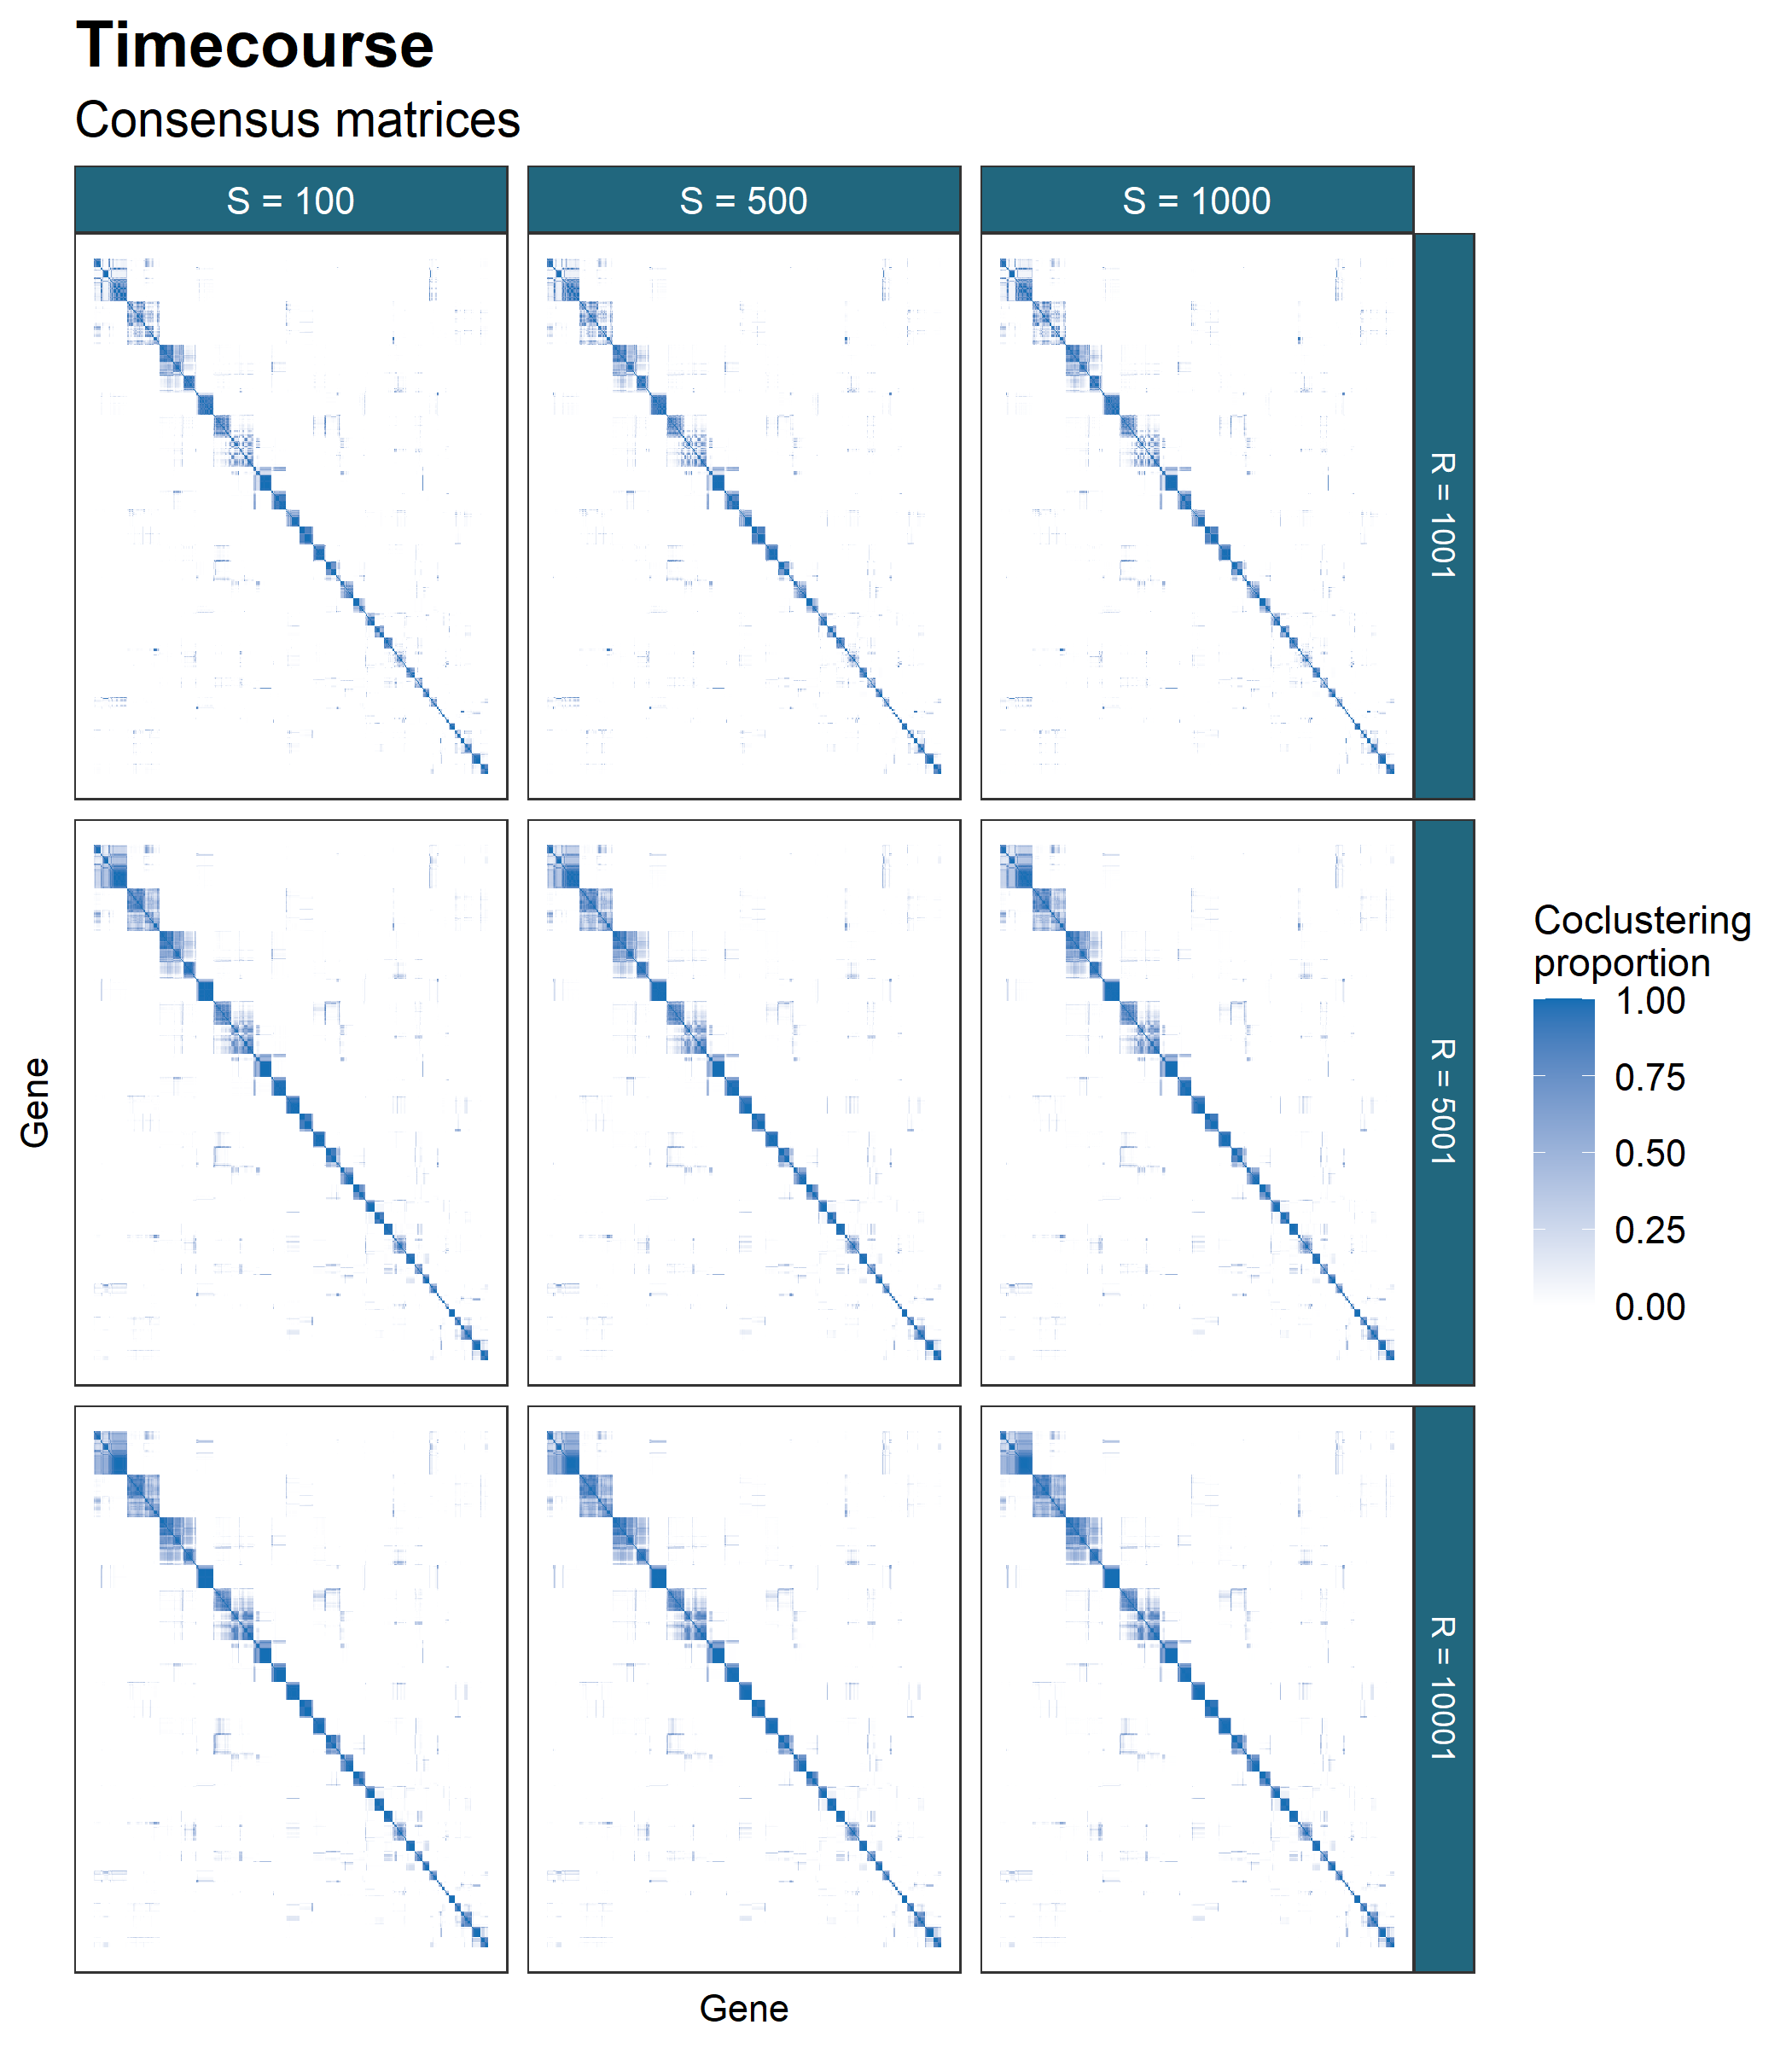
\includegraphics[scale=0.8]{./Images/Yeast/TimecourseCMcomparison.png}
	\caption{Consensus matrices for different ensembles of MDI for the Timecourse data. This dataset has stable clustering across the different choices of number of chains, $S$, and chain depth, $R$, with some components merging as the chain depth increases.}
	\label{fig:timecourseCMs}
\end{figure}

\begin{figure}
	\centering
	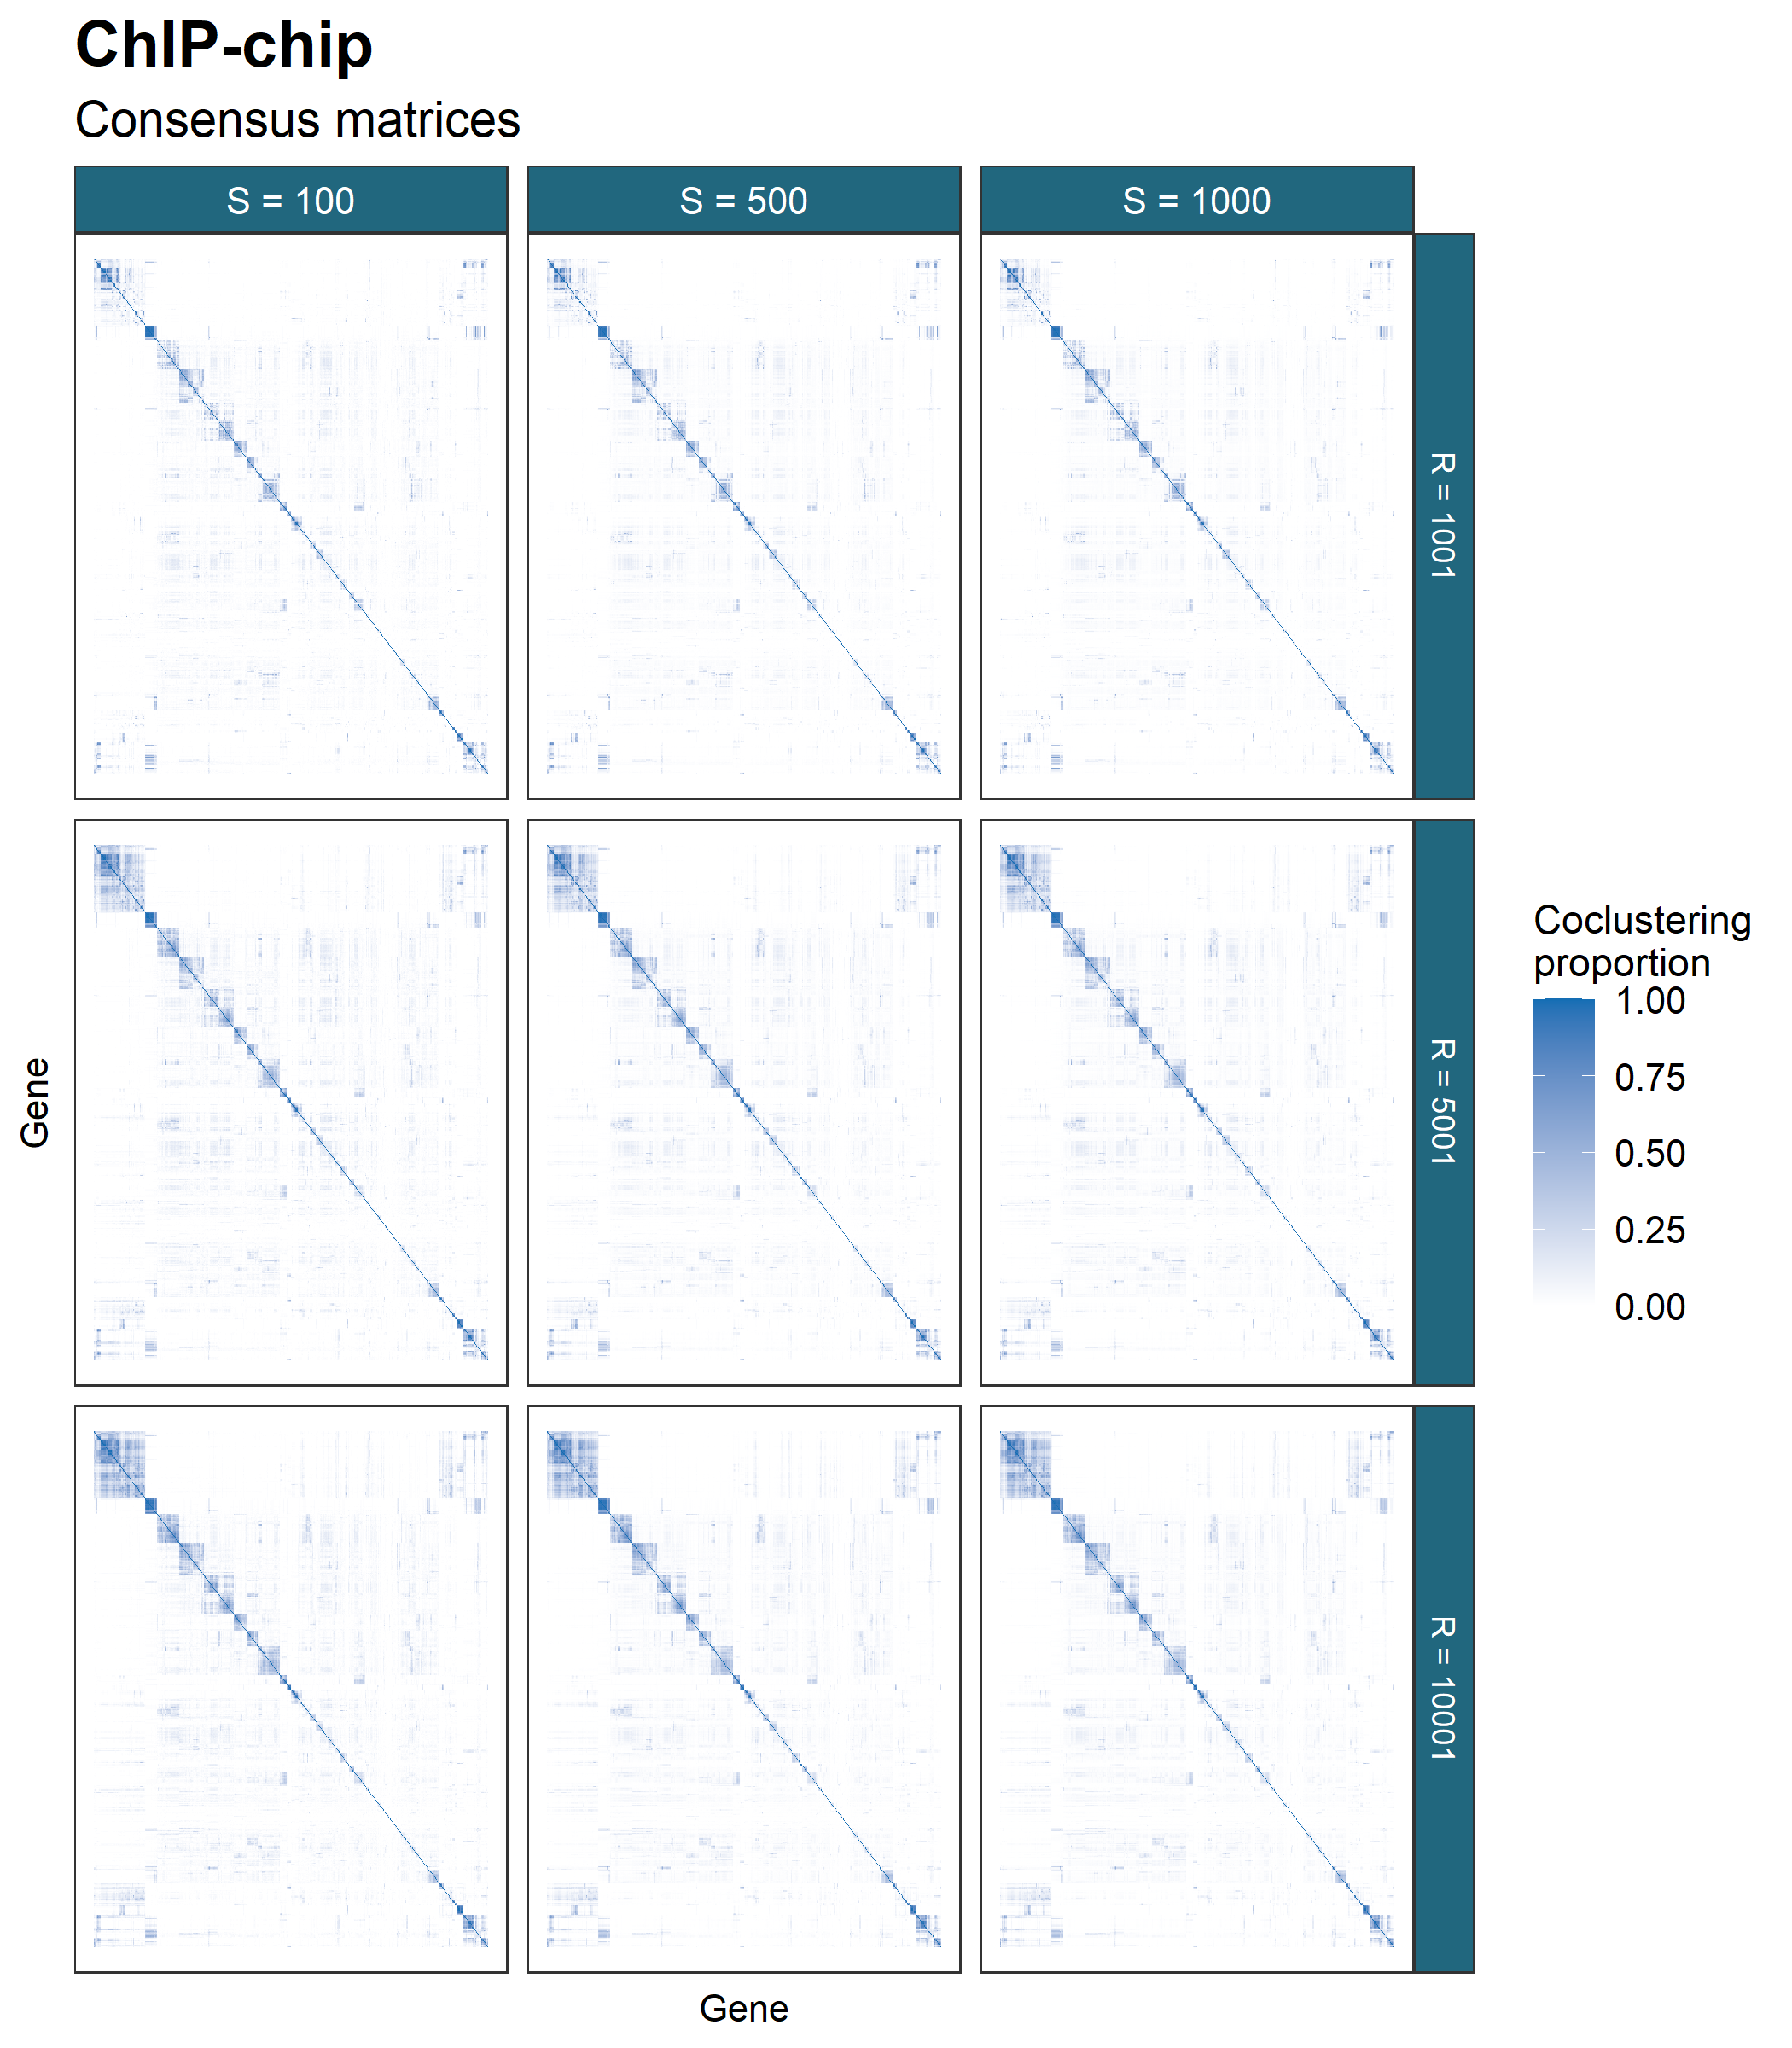
\includegraphics[scale=0.8]{./Images/Yeast/ChIP-chipCMcomparison.png}
	\caption{The ChIP-chip dataset is more sparse than the Timecourse data. In keeping with the results from the simulations for mixture models, deeper chains are required for better performance. It is only between $R=5,001$ and $R=10,001$ that no change in the clustering can be observed and the result is believed to be stable. In this dataset the number of chains used, $S$, appears relatively unimportant, with similar results for $S=100, 500, 1000$.}
	\label{fig:chipchipCMs}
\end{figure}

\begin{figure}
	\centering
	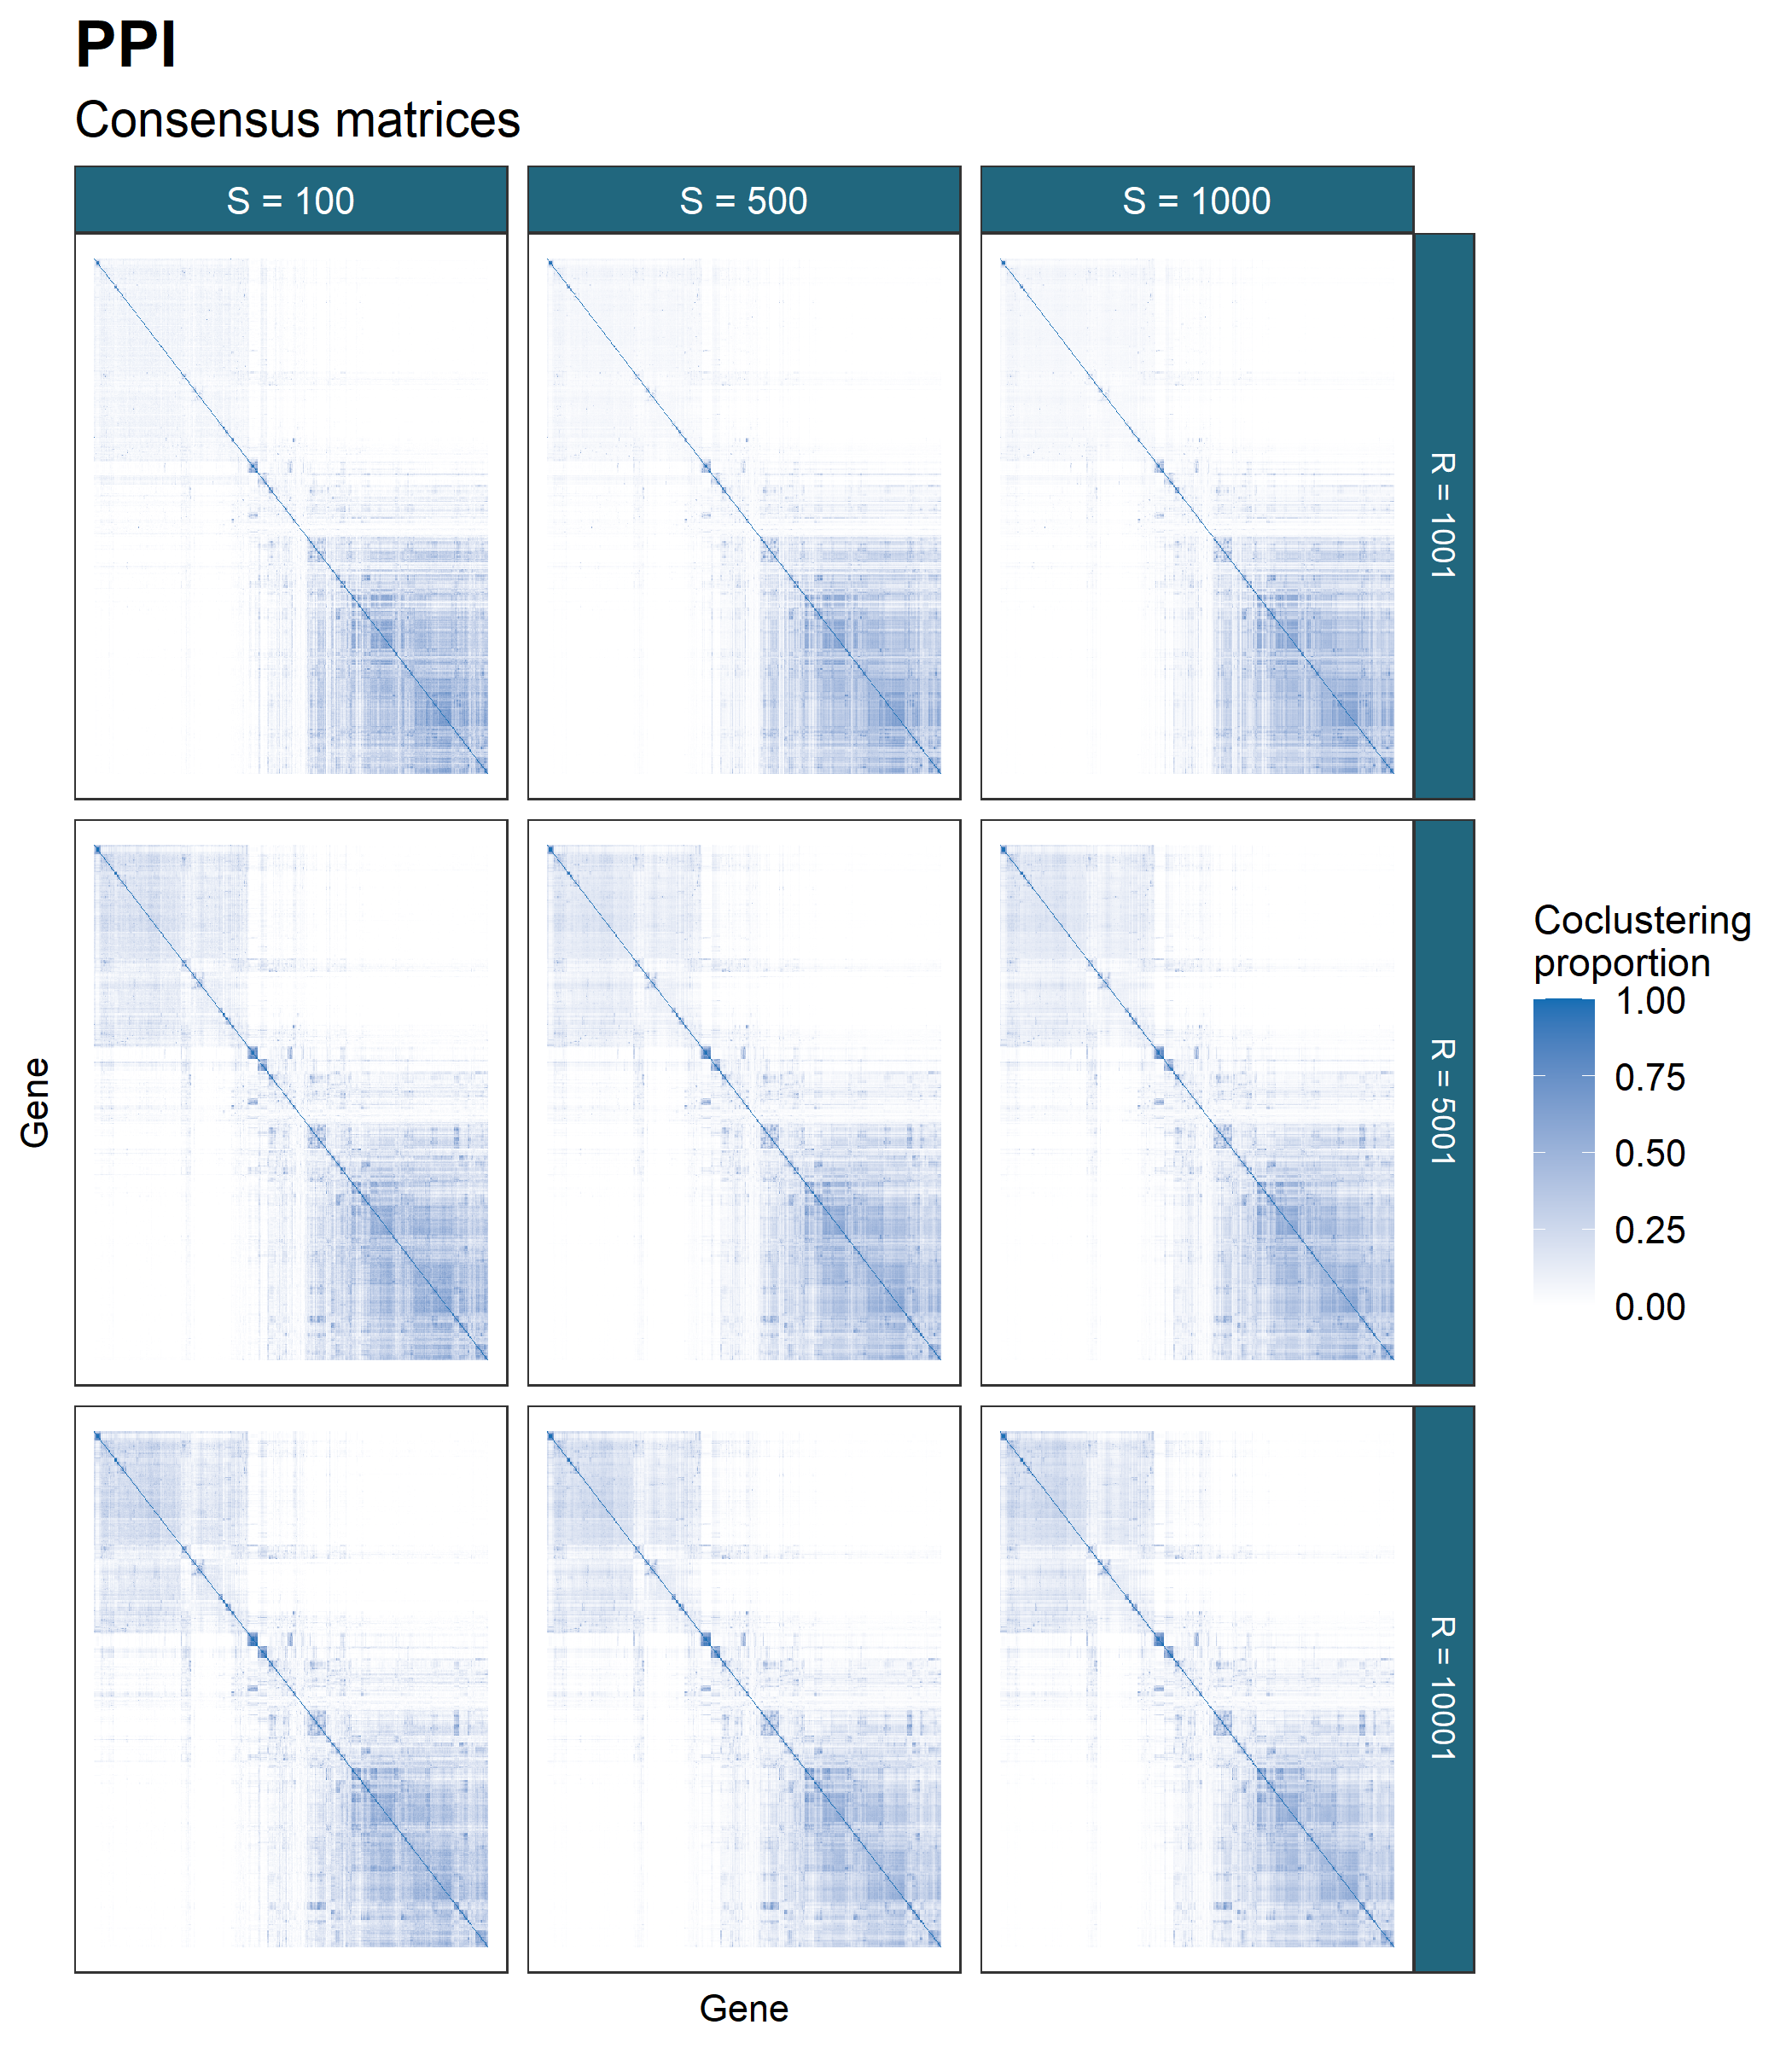
\includegraphics[scale=0.8]{./Images/Yeast/PPICMcomparison.png}
	\caption{The PPI dataset has awkward characteristics for modelling. A wide, sparse dataset it is chain depth that we found to be the most important parameter for the ensemble. Similar to the results in figure \ref{fig:chipchipCMs}, the matrices only stabilise from $R=5001$ to $R=10001$.}
	\label{fig:ppiCMs}
\end{figure}


\subsection{Bayesian analysis} \label{sec:yeastBayesianAnalysis}
We ran 10 chains of MDI for 36 hours saving every thousandth sample. This resulted in chains of varying length. We reduced the chains to 676 samples as this was the number of samples achieved by the slowest chain. Similar to section \ref{sec:simBayesianAnalysis} these chains were then investigated for 
\begin{itemize}
	\item within-chain stationarity using the Geweke convergence diagnostic \citep{geweke1991evaluating}, and
	\item across-chain convergence using $\hat{R}$ \citep{gelman1992inference} and the Vats-Knudson extension \citep[\emph{stable $\hat{R}$},][]{vats2018revisiting}.
\end{itemize}
%The Geweke convergence diagnostic is a standard Z-score; it compares the sample mean of two sets of samples (in this case buckets of samples from the first half of the samples to the sample mean of the entire second half of samples). It is calculated under the assumption that the two parts of the chain are asymptotically independent and if this assumption holds than the scores are expected to be standard normally distributed presenting evidence for within chain stationarity.
%
%$\hat{R}$ is expected to approach 1.0 if the set of chains are converged. Low $\hat{R}$ is not sufficient in itself to claim chain convergence, but values above 1.1 are clear evidence for a lack of convergence \citep{gelman2013bayesian}. \cite{vats2018revisiting} show that this threshold is significantly too high (1.01 being a better choice) and propose extensions to $\hat{R}$ that enable a more formal rule for a threshold. It is their method as implemented in the R package \texttt{stableGR} \citep{knudson20202stableGR} that is the final check of convergence.
%
Again we focus upon stationarity of the continuous variables. In the implementation of MDI we used, the recorded continuous variables are the concentration parameters of the Dirichlet distribution for the dataset-specific component weights and the $\phi_{ij}$ parameter associated with the correlation between the $i^{th}$ and $j^{th}$ datasets. 
\begin{figure}
	\centering
	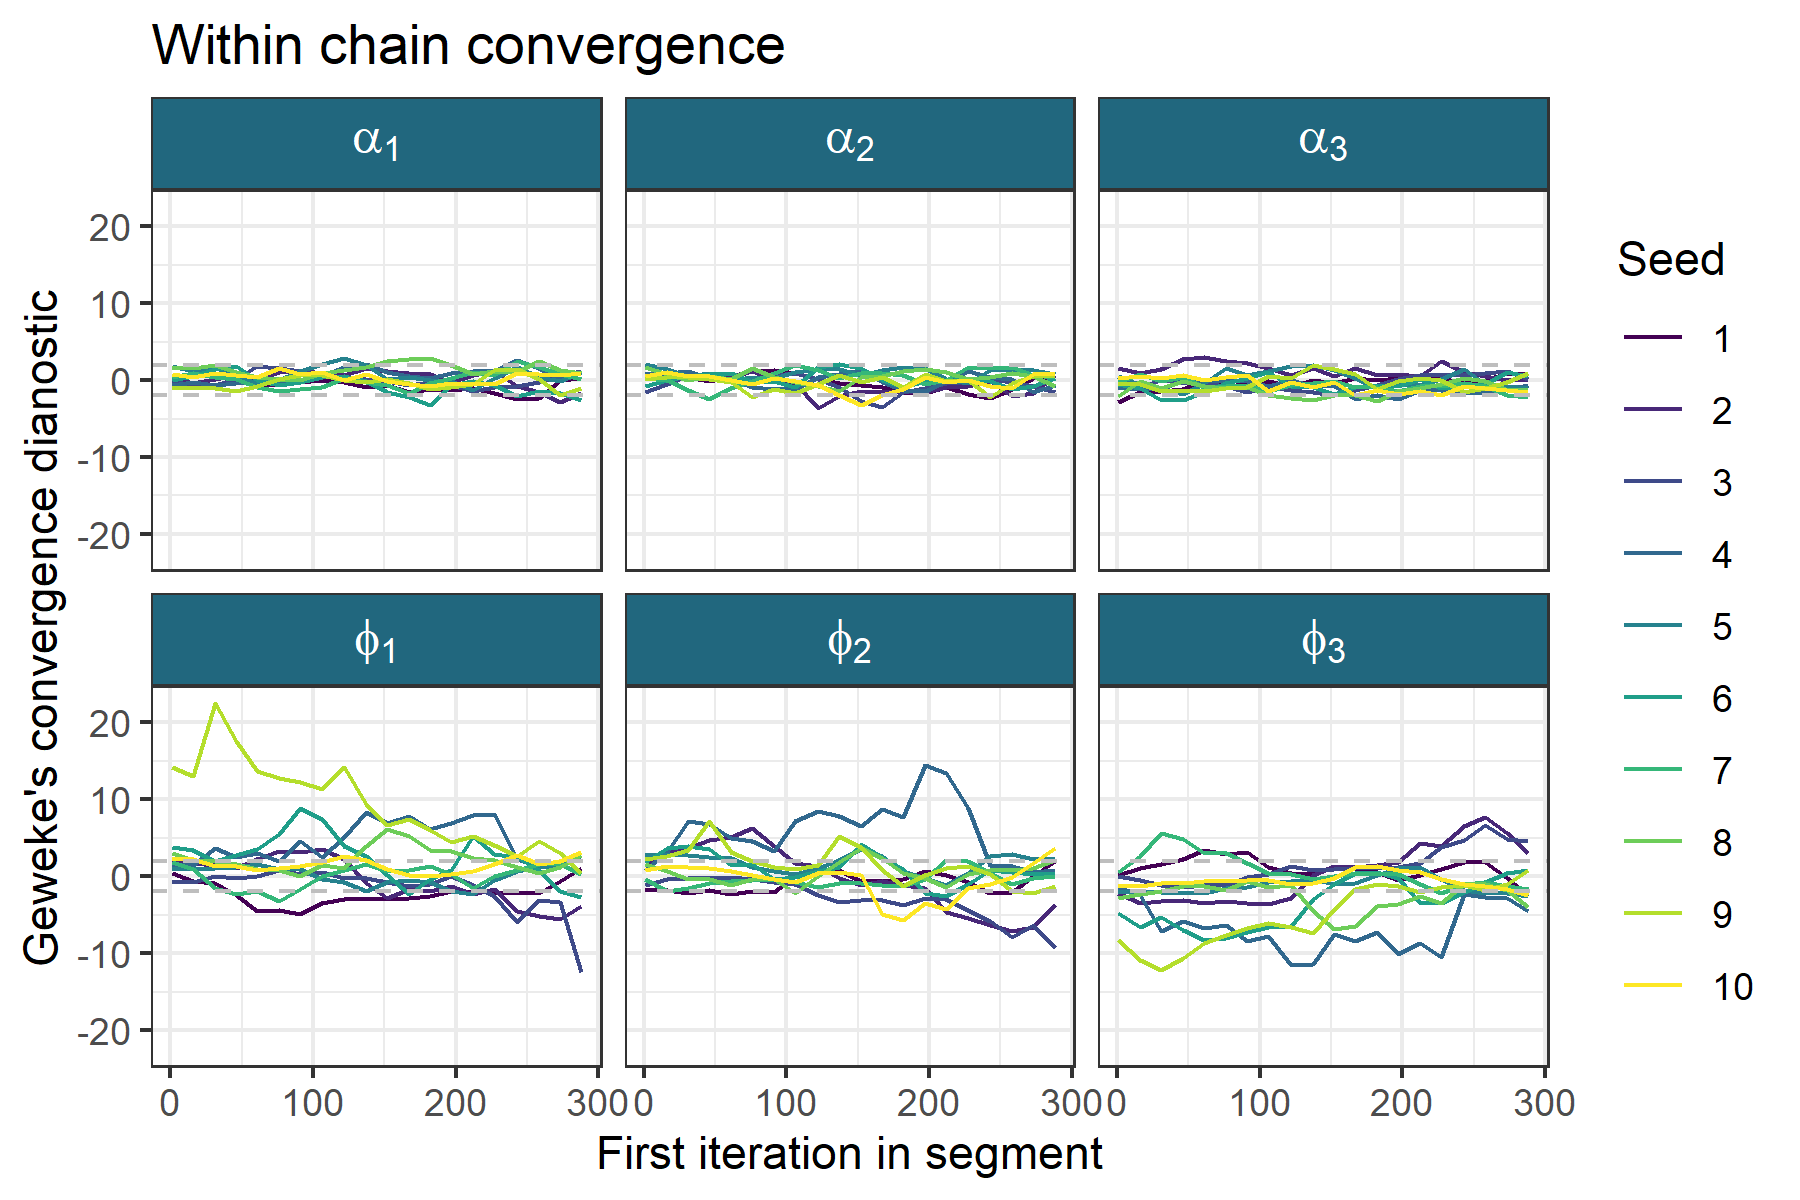
\includegraphics[scale=1.0]{./Images/Yeast/Convergence/gewekePlot.png}
	\caption{Chain 9 can be seen to have the most extreme behaviour in the distribution of the Geweke diagnostic for the parameters. We remove this chain from the analysis. Of the remaining chains we believe that 1, 2, 4 and 6 express the distributions furthest removed from the desired behaviour and are dropped from the analysis.}
	\label{fig:gewekePlot}
\end{figure}

%\begin{figure}
%	\centering
%	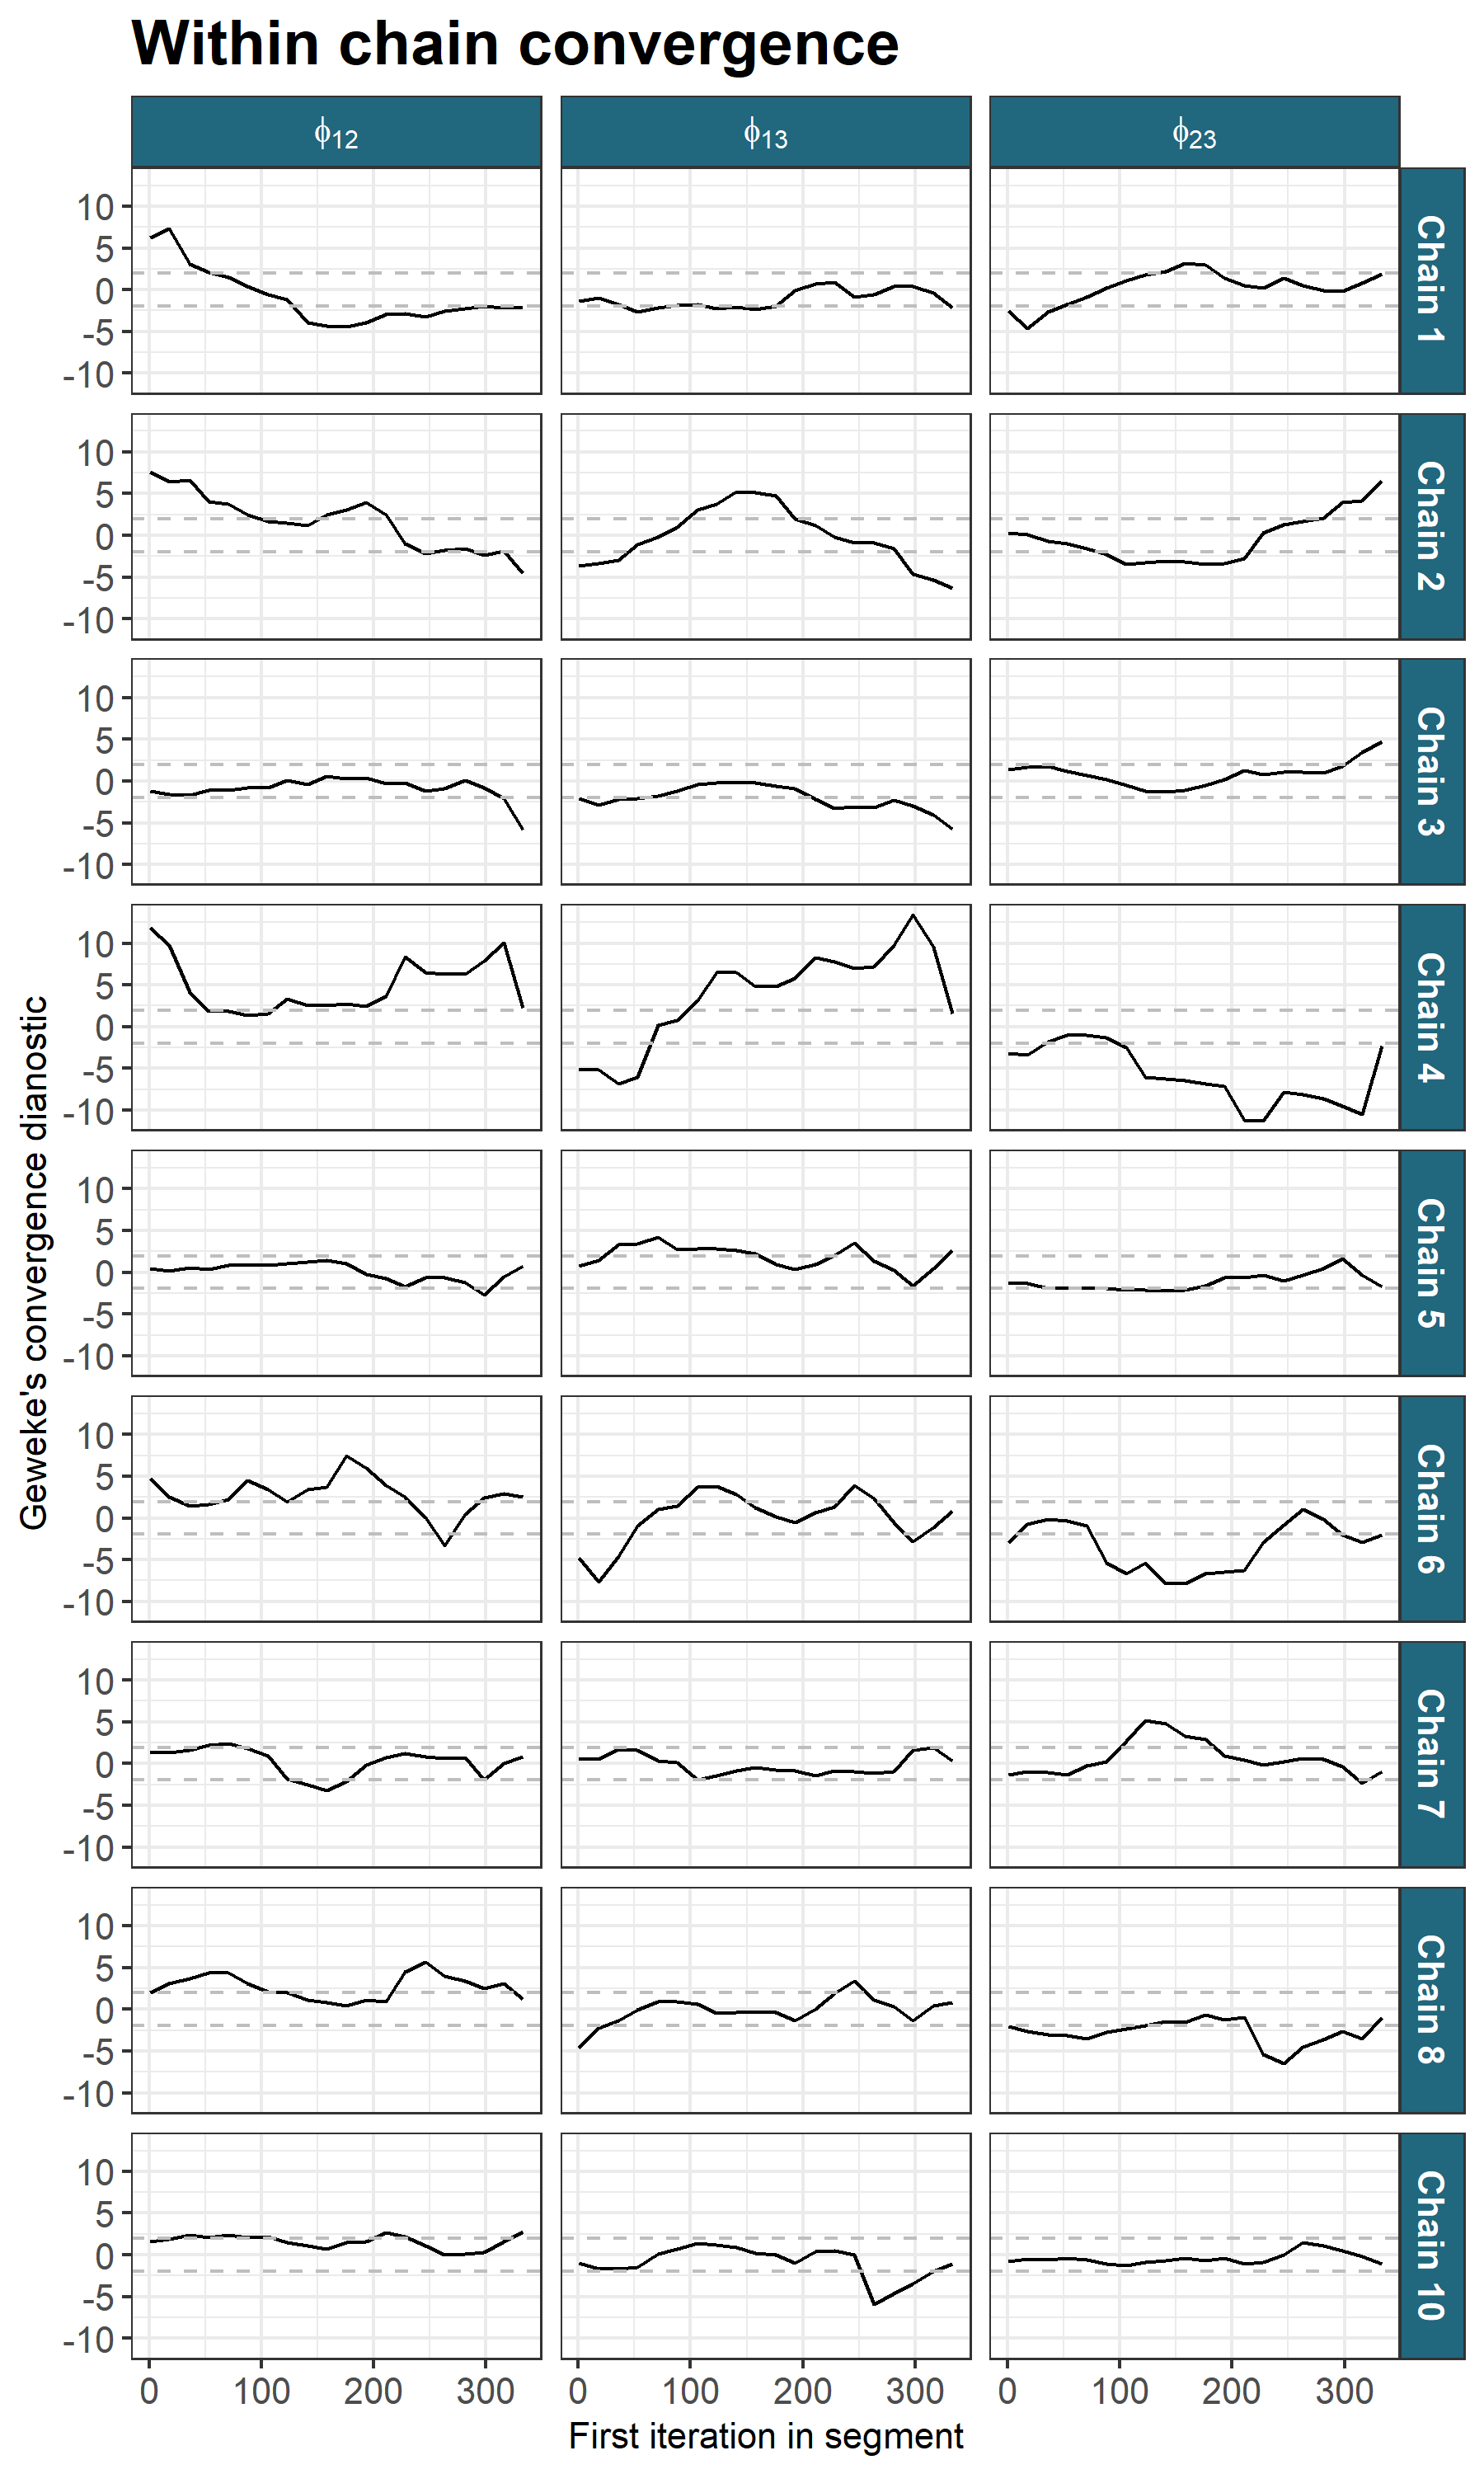
\includegraphics[scale=0.7]{./Images/Yeast/Convergence/gewekePhiChain.png}
%	\caption{None of the chains appear to be standard normal in their distribution. Chain 4 behaves very strangely and is also dropped from the analysis. Of the remaining chains there is less clear distinctions, but chains 1, 2, and 6 appear most extreme and thus are dropped.}
%	\label{fig:gewekePhiPlot}
%\end{figure}
We plot the Geweke-statistic for each chain in figure \ref{fig:gewekePlot}. No chain is perfectly behaved; as we cannot reduce to the set of stationary chains we thus exclude the most poorly behaved chains. Our lack of belief in the convergence of these chains is fortified by the behaviour of $\hat{R}$ (which can be seen in figure \ref{fig:gelmanPlot}) and the different distributions sampled for the $\phi_{lm}$ parameters shown in figure \ref{fig:bayesDensities}.
%where the values of $\hat{R}$ do not drop below 1.25 for the $\phi$ parameters. Stable $\hat{R}$ is also too high, with several million more samples recommended before convergence is expected.
\begin{figure}
	\centering
	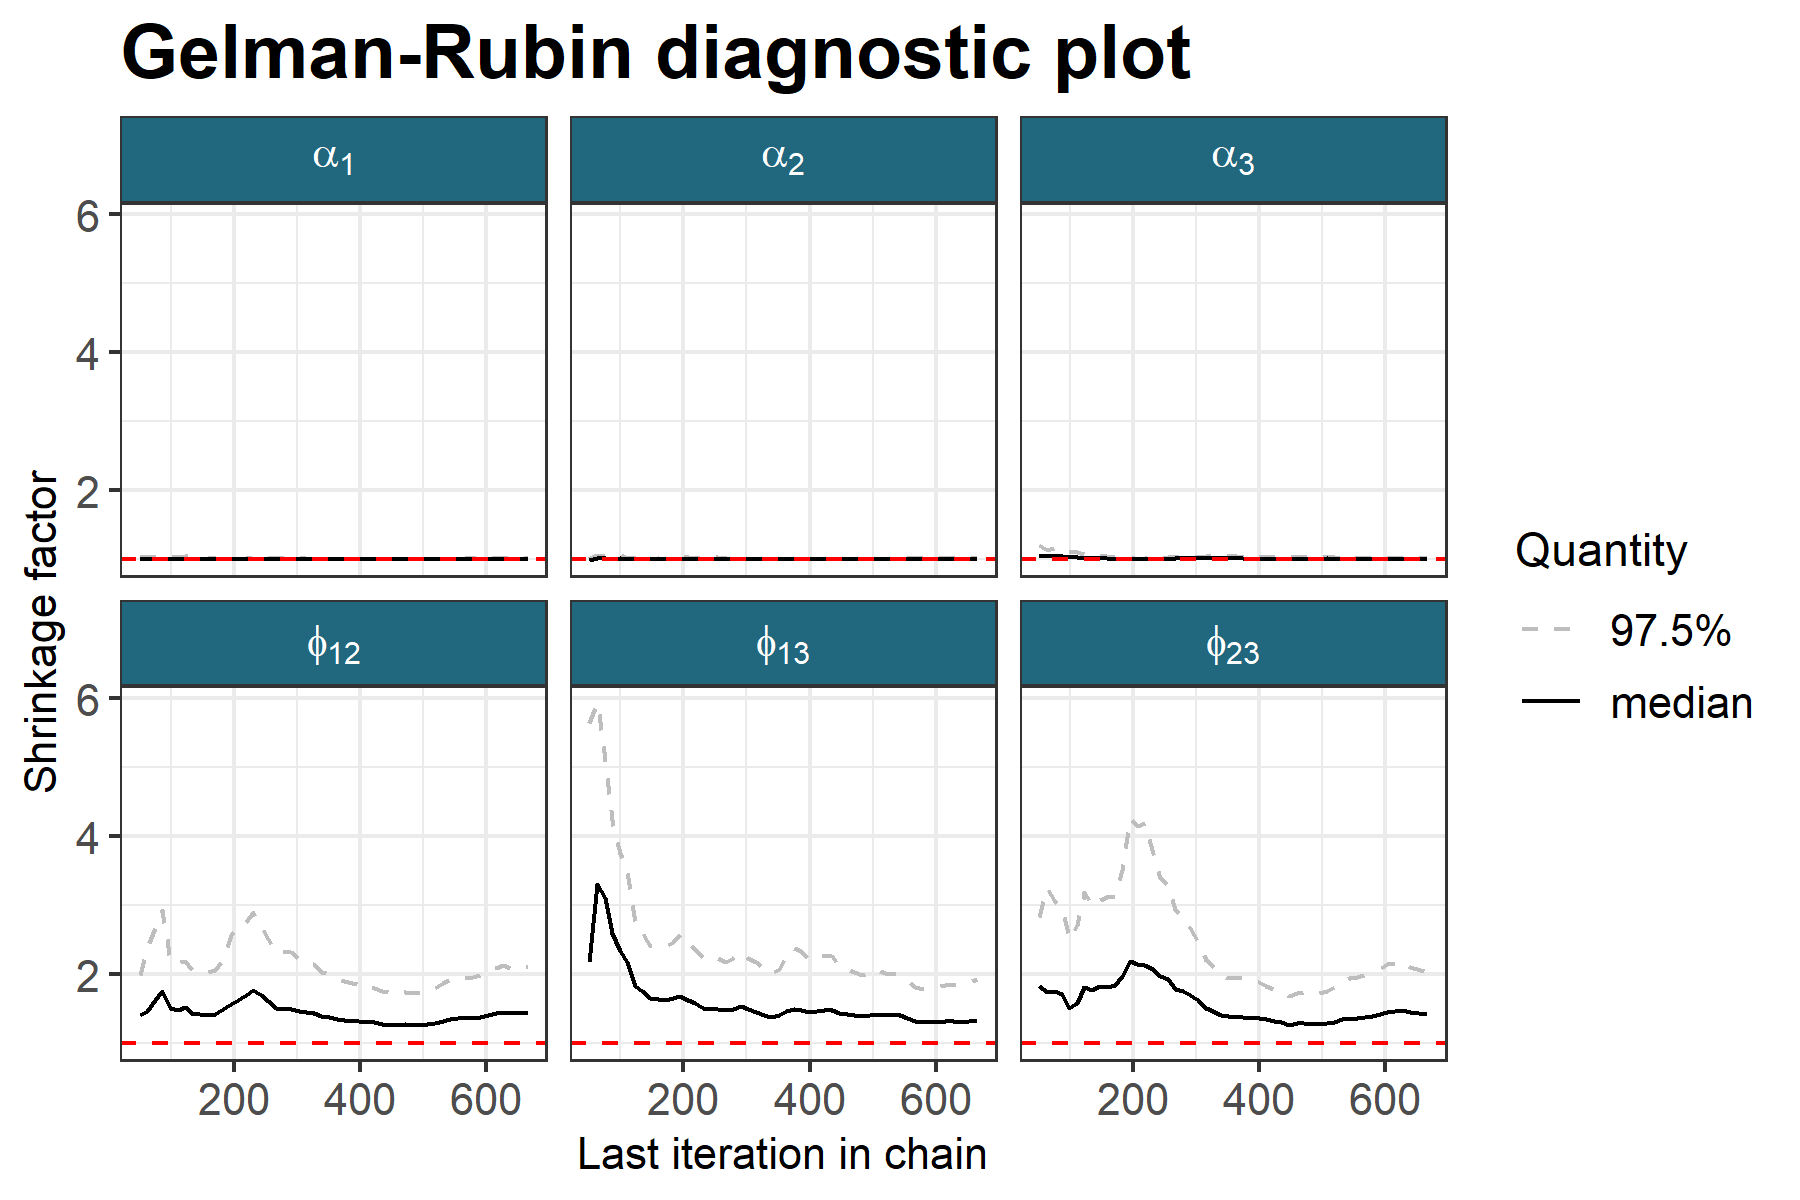
\includegraphics[scale=1.0]{./Images/Yeast/Convergence/gelmanPlot.png}
	\caption{The chains still appear to be unconverged with $\hat{R}$ remaining above 1.25 for the $\phi_{12}, \phi_{13}$ and $\phi_{23}$ parameters. Stable $\hat{R}$ is also too high with values of 1.049, 1.052 and 1.057 for $\phi_{12}, \phi_{13}$ and $\phi_{23}$ respectively.}
	\label{fig:gelmanPlot}
\end{figure}
\begin{figure}
	\centering
	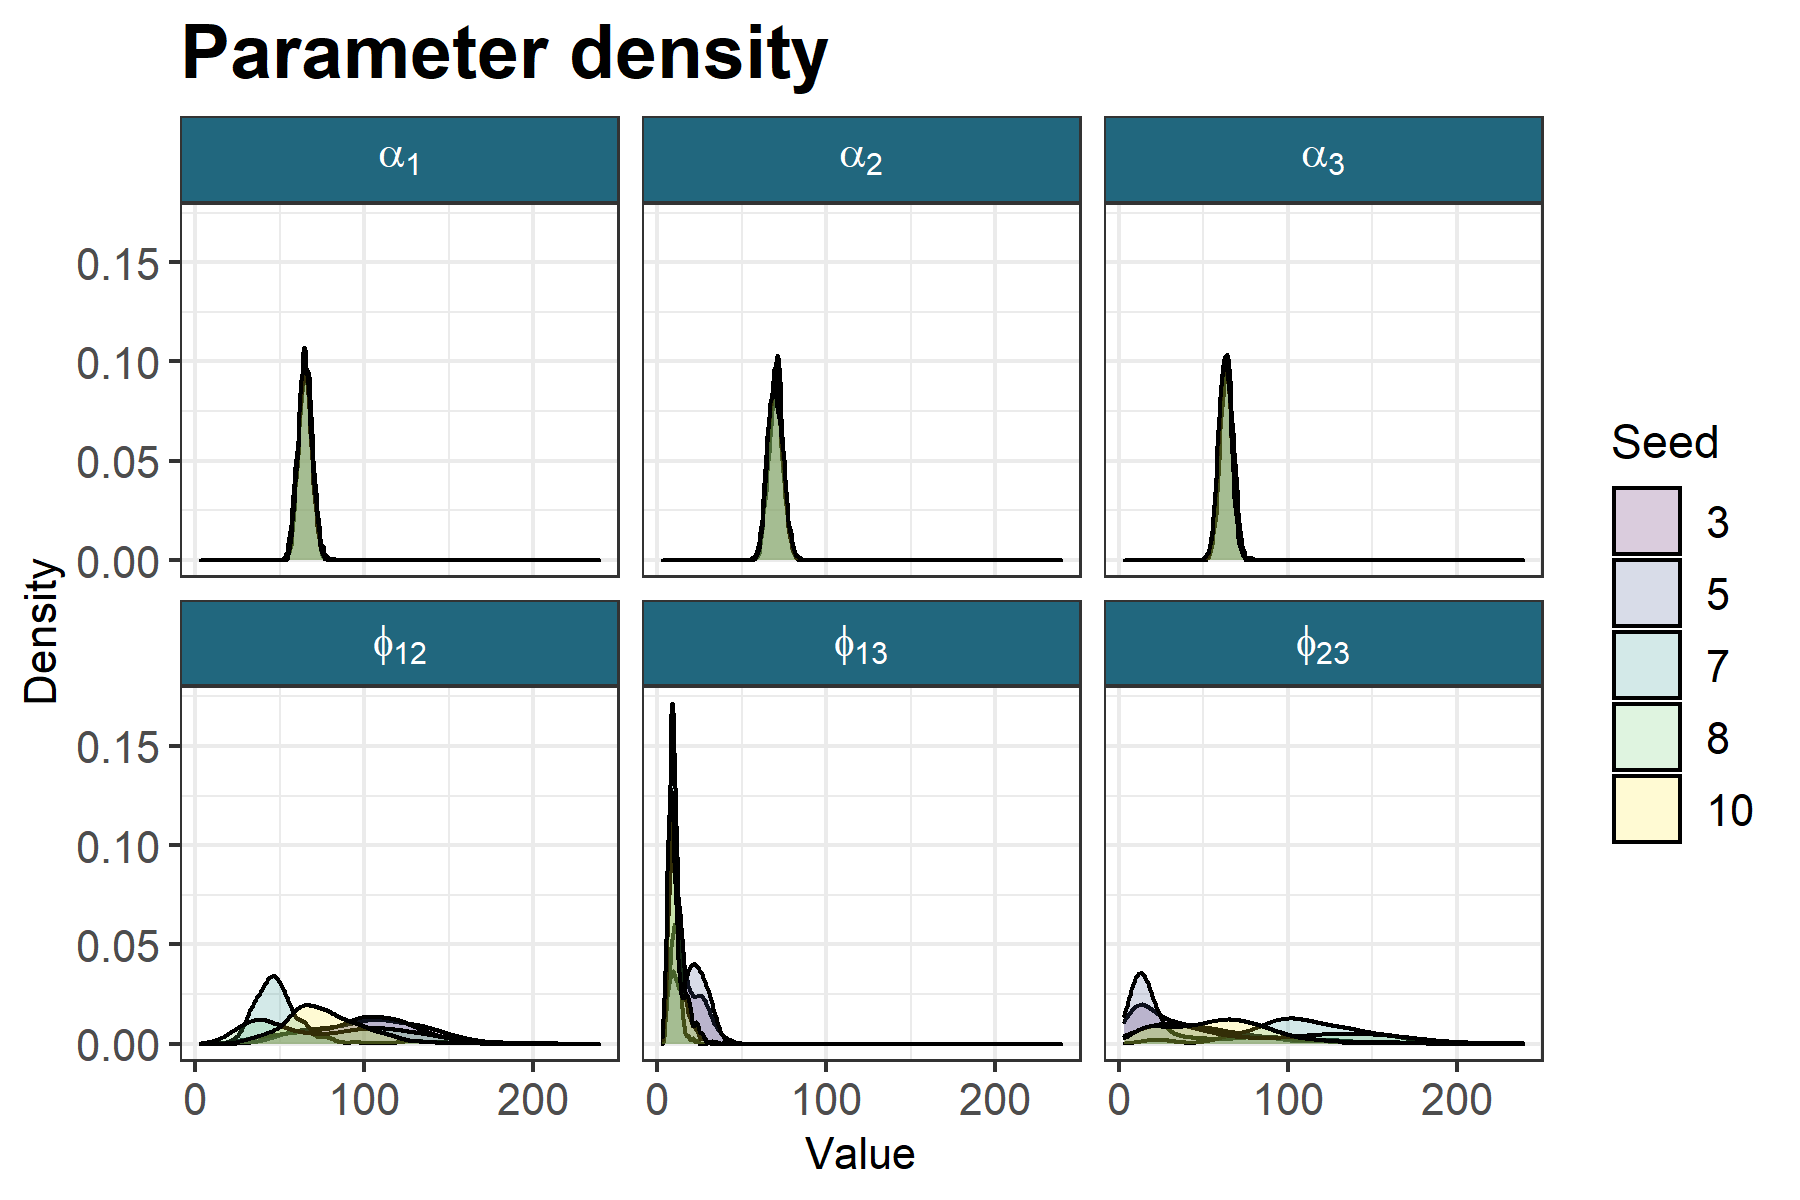
\includegraphics[scale=1]{./Images/Yeast/densityPlotReduced.png}
	\caption{The densities of the continuous variables across the 5 chains kept for analysis. The mean sampled values are $\alpha_1= 64.84$, $\alpha_2 = 69.85$, $\alpha_2 = 63.22$, $\phi_{12} = 81.76$, $\phi_{13} = 13.87$, and $\phi_{23} = 65.03$. It can be seen that different modes are being sampled for the $\phi$ parameters in each chain.
	}
	\label{fig:bayesDensities}
\end{figure}

We visualise the the PSMs for each dataset in figure \ref{fig:yeastPSMs}. 
%The Timecourse data appears to have only the mildest of disagreement between the PSMs from different chains (see figure \ref{fig:timecoursePSMs}). The lack of convergence between chains emerges in the ChIP-chip data (figure \ref{fig:chipchipPSMs}) and, to a far greater degree, in the PPI data (figure \ref{fig:ppiPSMs}).

\begin{figure}
	\centering
	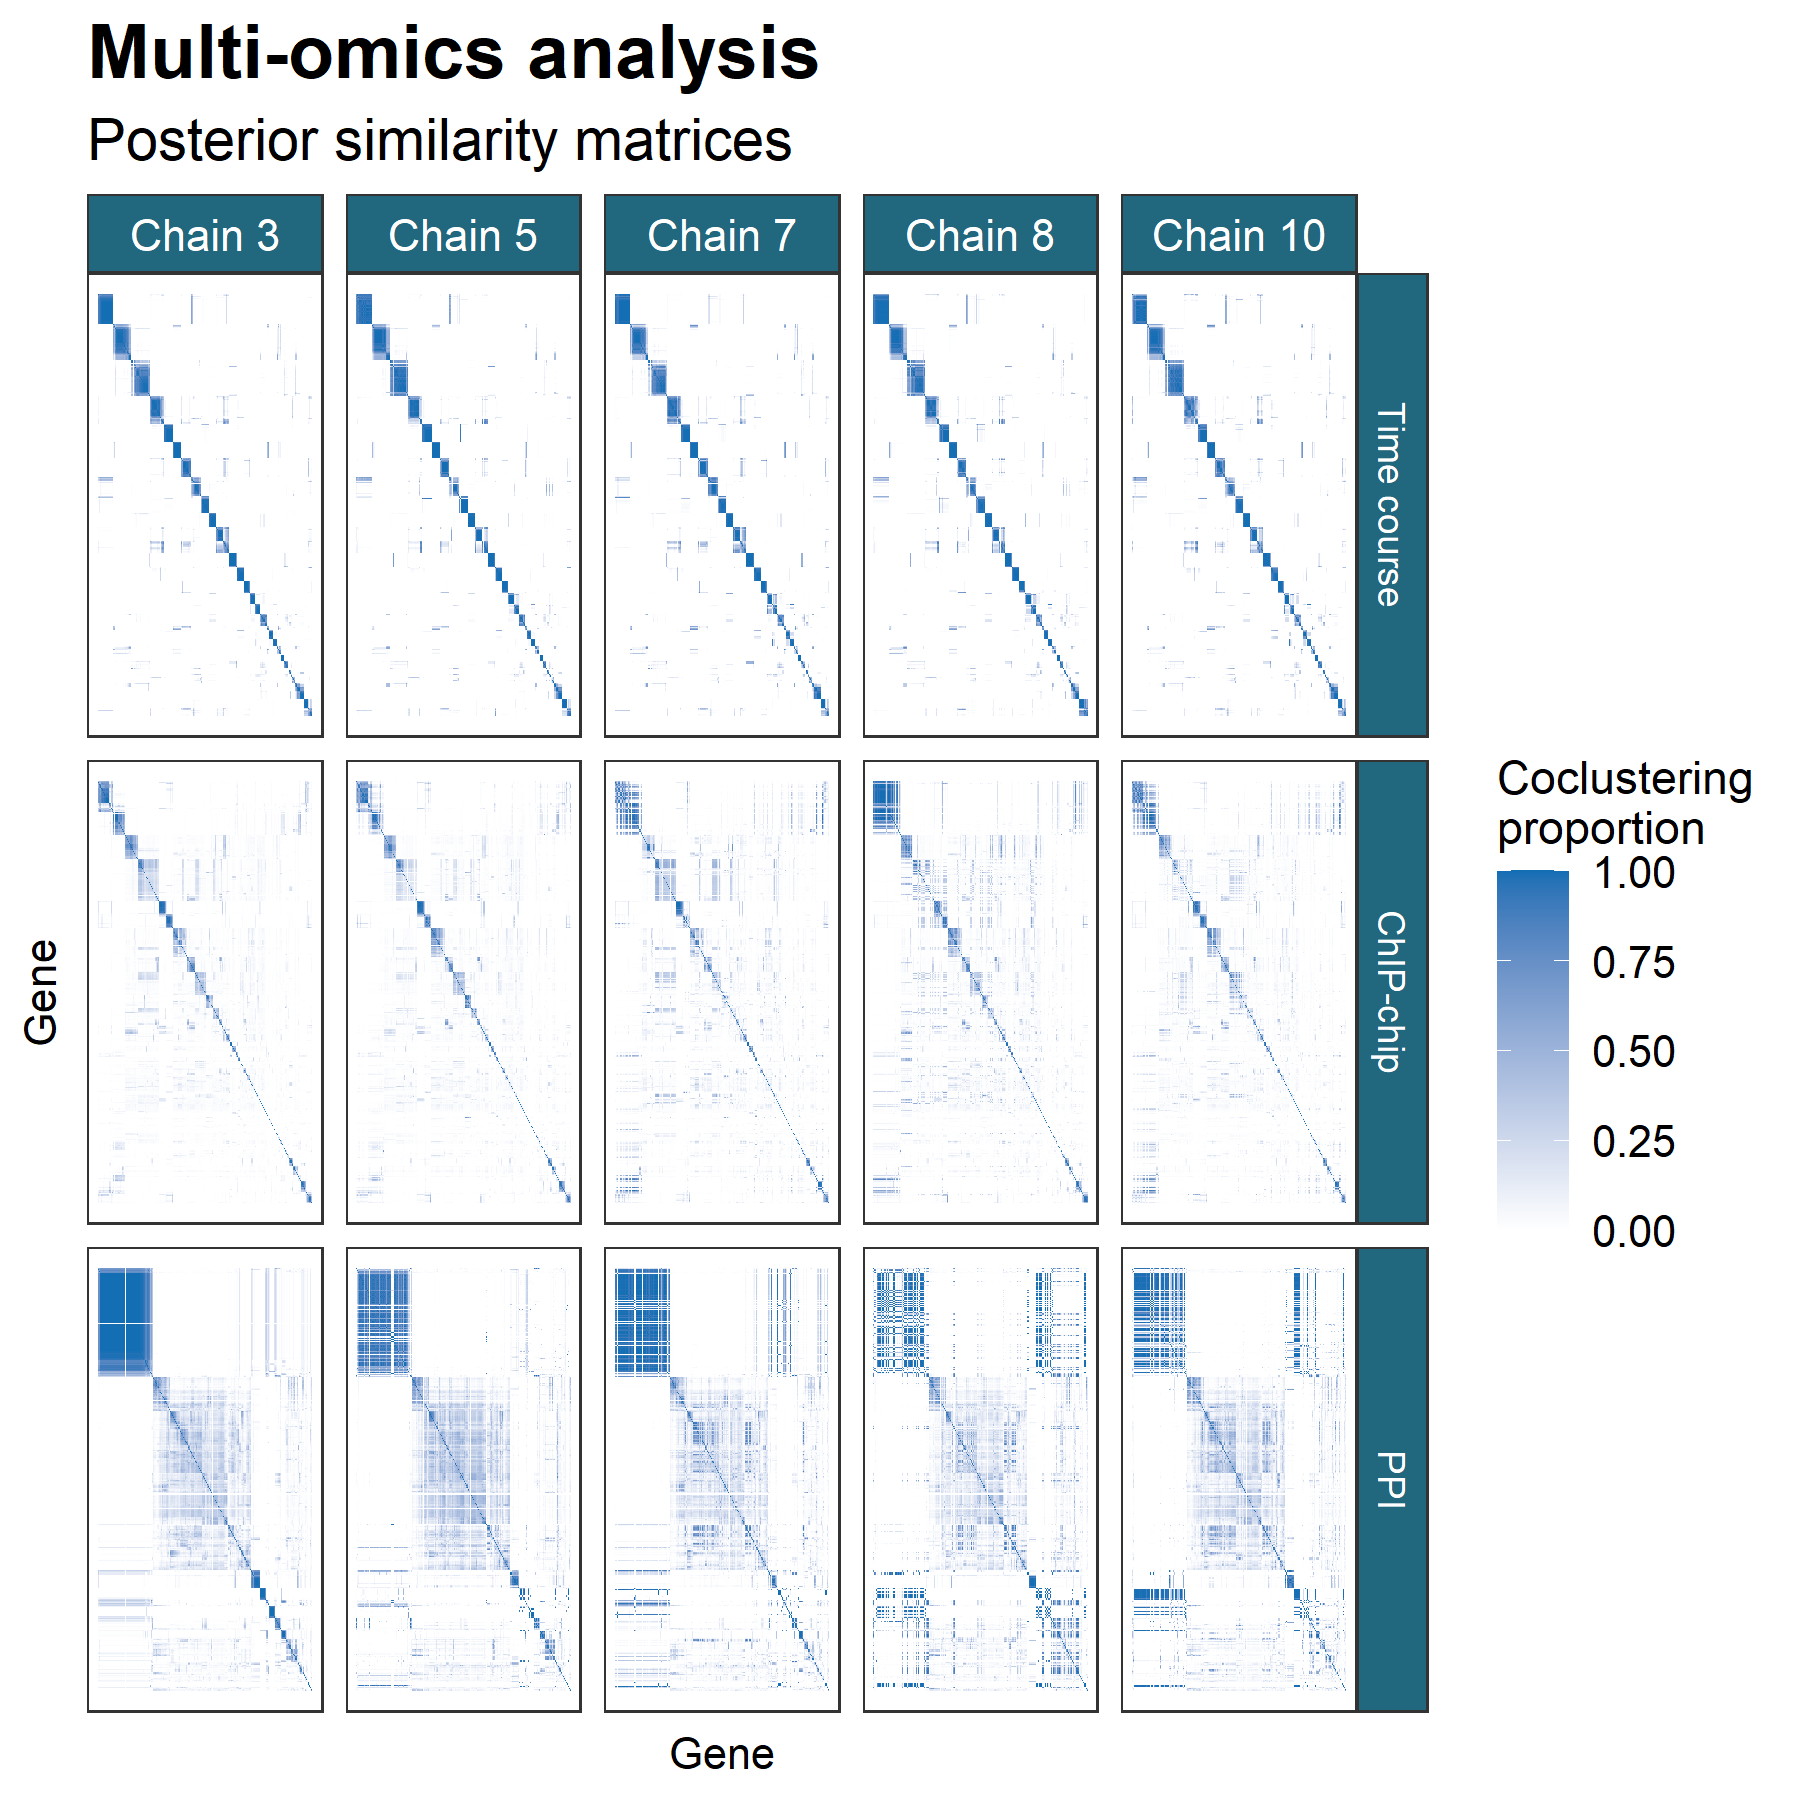
\includegraphics[scale=1.0]{./Images/Yeast/YeastPSMcomparisonReduced.png}
	\caption{PSMs for each chain within each dataset. The PSMs are ordered by hierarchical clustering of the rows of the PSM for chain 3 in each dataset. There is no marked difference between the matrices for the Timecourse data with disagreement becoming more prominent in the ChIP-chip data and more so again in the PPI dataset.}
	\label{fig:yeastPSMs}
\end{figure}


%\begin{figure}
%	\centering
%	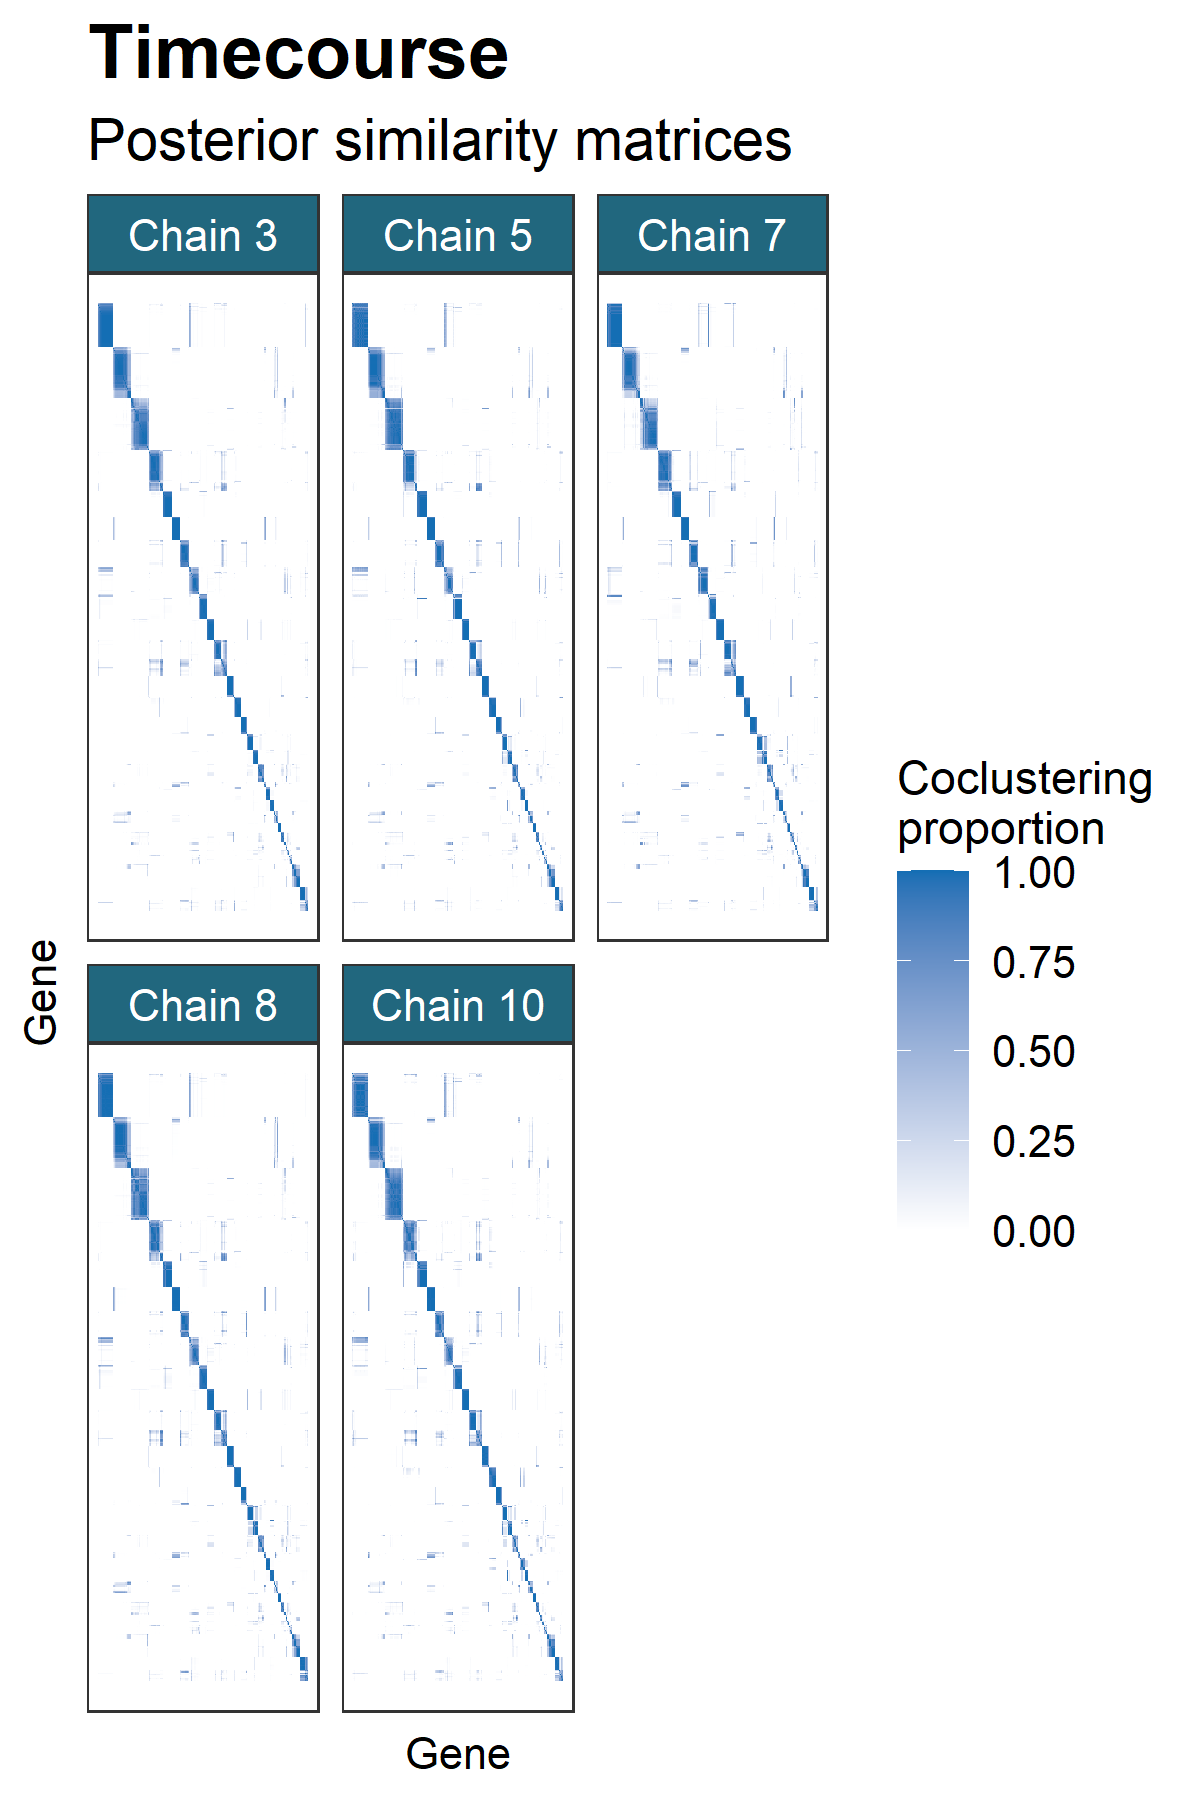
\includegraphics[scale=0.5]{./Images/Yeast/TimecoursePSMcomparisonReduced.png}
%	\caption{The entries of each matrix are ordered by hierarchical clustering of the PSM for chain 3. There is no marked difference between matrices.}
%	\label{fig:timecoursePSMs}
%\end{figure}

%\begin{figure}
%	\centering
%	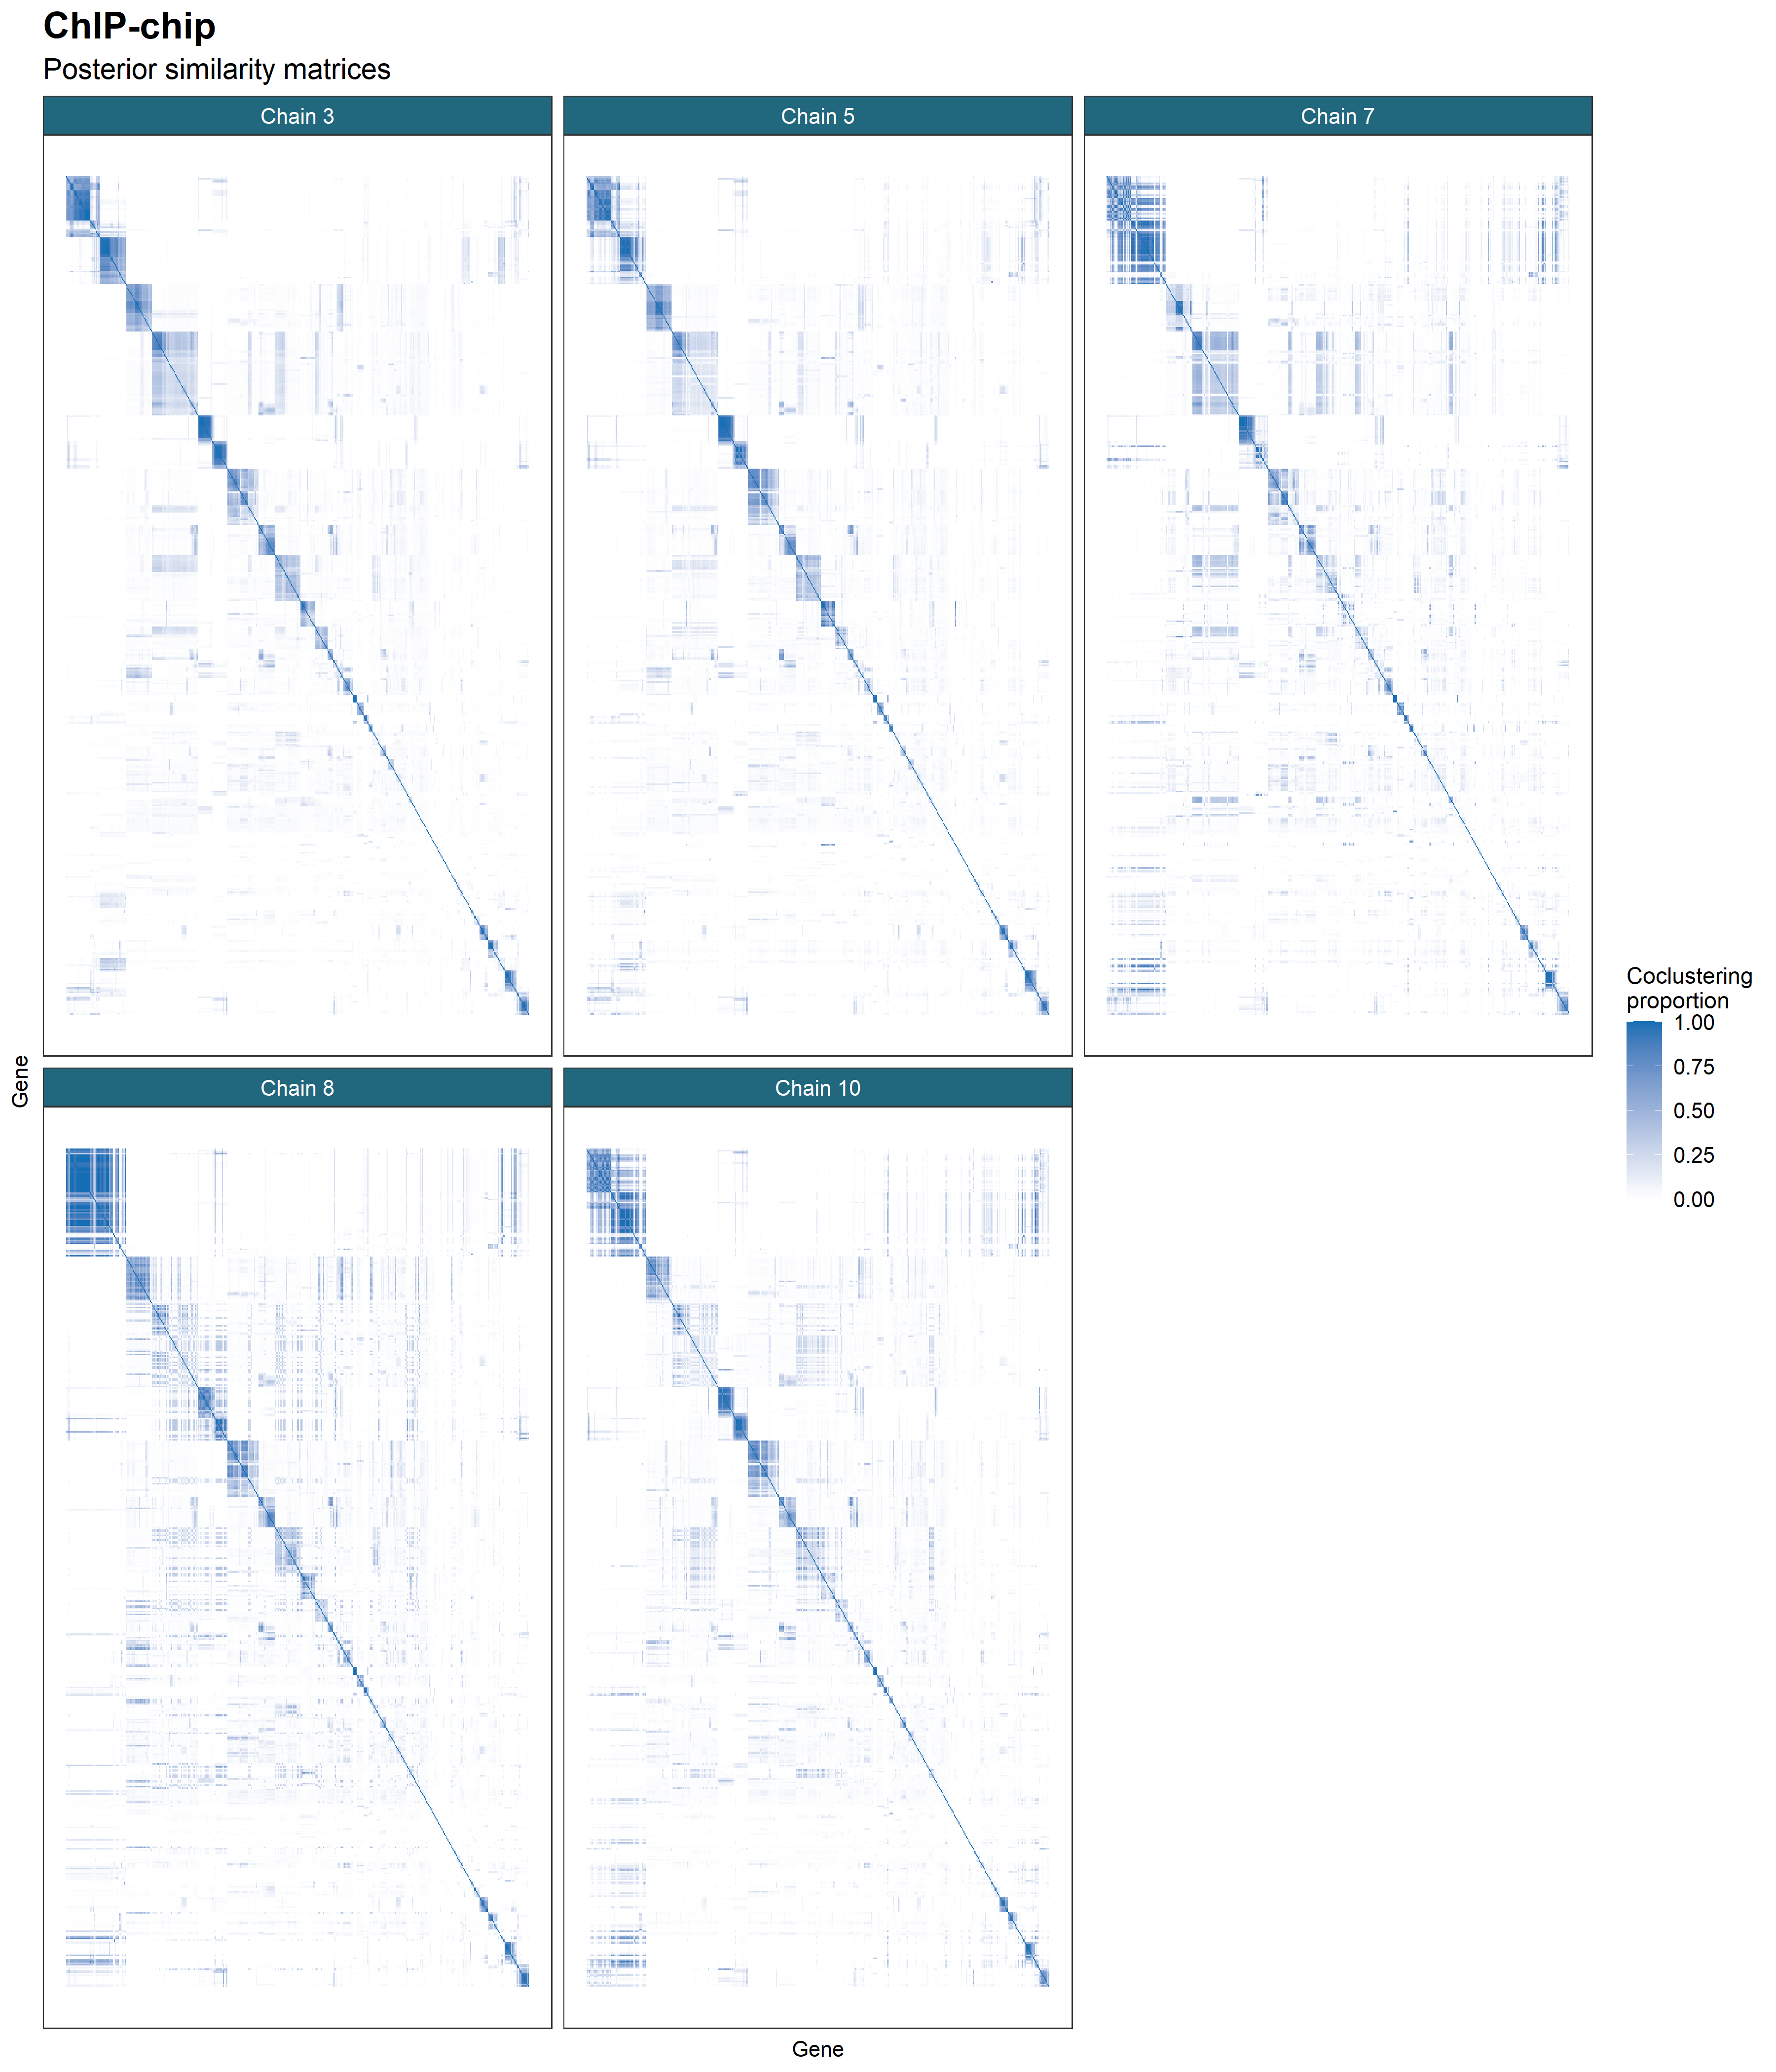
\includegraphics[scale=0.5]{./Images/Yeast/ChIP-chipPSMcomparisonReduced.png}
%	\caption{The entries of each matrix are ordered by hierarchical clustering of the PSM for chain 3. Disagreement can be seen between each chain.}
%	\label{fig:chipchipPSMs}
%\end{figure}

%\begin{figure}
%	\centering
%	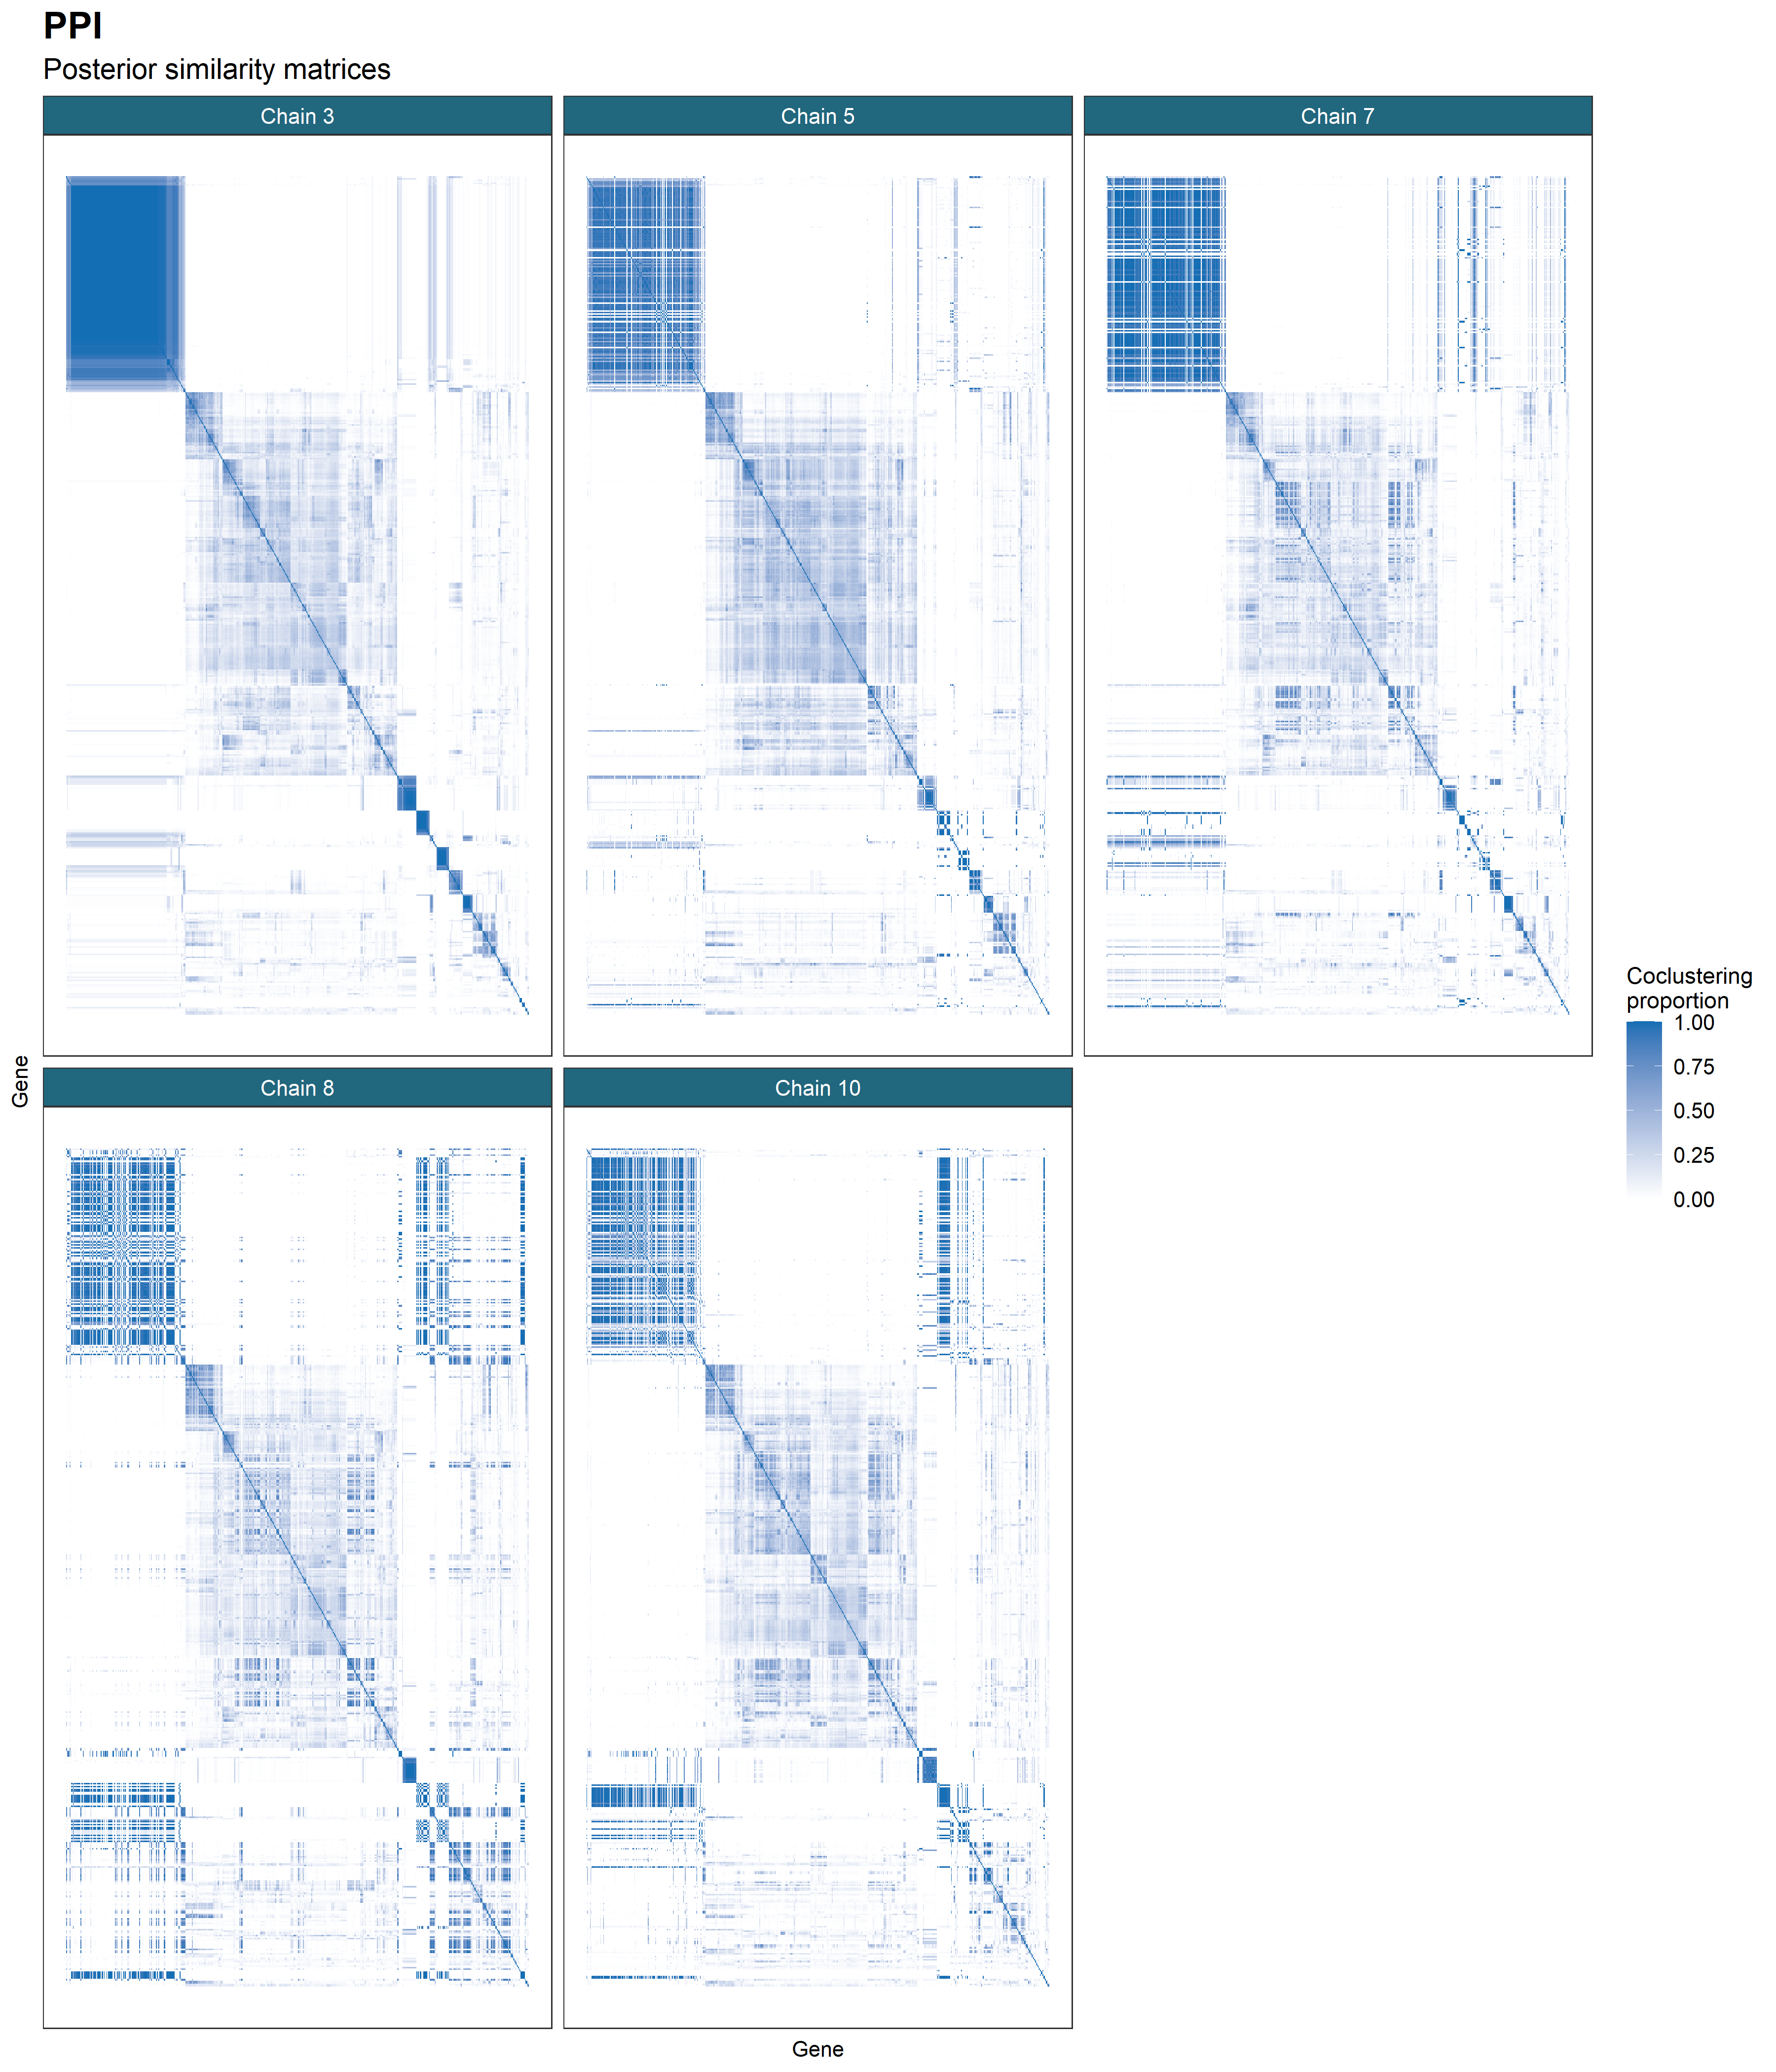
\includegraphics[scale=0.5]{./Images/Yeast/PPIPSMcomparisonReduced.png}
%	\caption{The entries of each matrix are ordered by hierarchical clustering of the PSM for chain 3. These PSMs express very large disagreement about the clustering. There is some agreement with the square in the centre of each plot appearing similar in each PSM. However, the other sections (which consist of the most confident allocations) appear to completely fail to overlap.}
%	\label{fig:ppiPSMs}
%\end{figure}

If we compare the distribution of sampled values for the $\phi$ parameters for the Bayesian chains that we keep based upon their convergence diagnostics, the final ensemble used ($R=10001$, $S=1000$) and the pooled samples from the 5 long chains, then we see that the ensemble consisting of the long chains (which might be believed to sampling different parts of the posterior distribution) is closer in its appearance to the distributions sampled by the Consensus clustering than to any single chain. There is no consistent distribution across the chains, but it appears that Consensus clustering is producing a distribution that does have similar behaviour to the overlap of the chains.

\begin{figure}
	\centering
	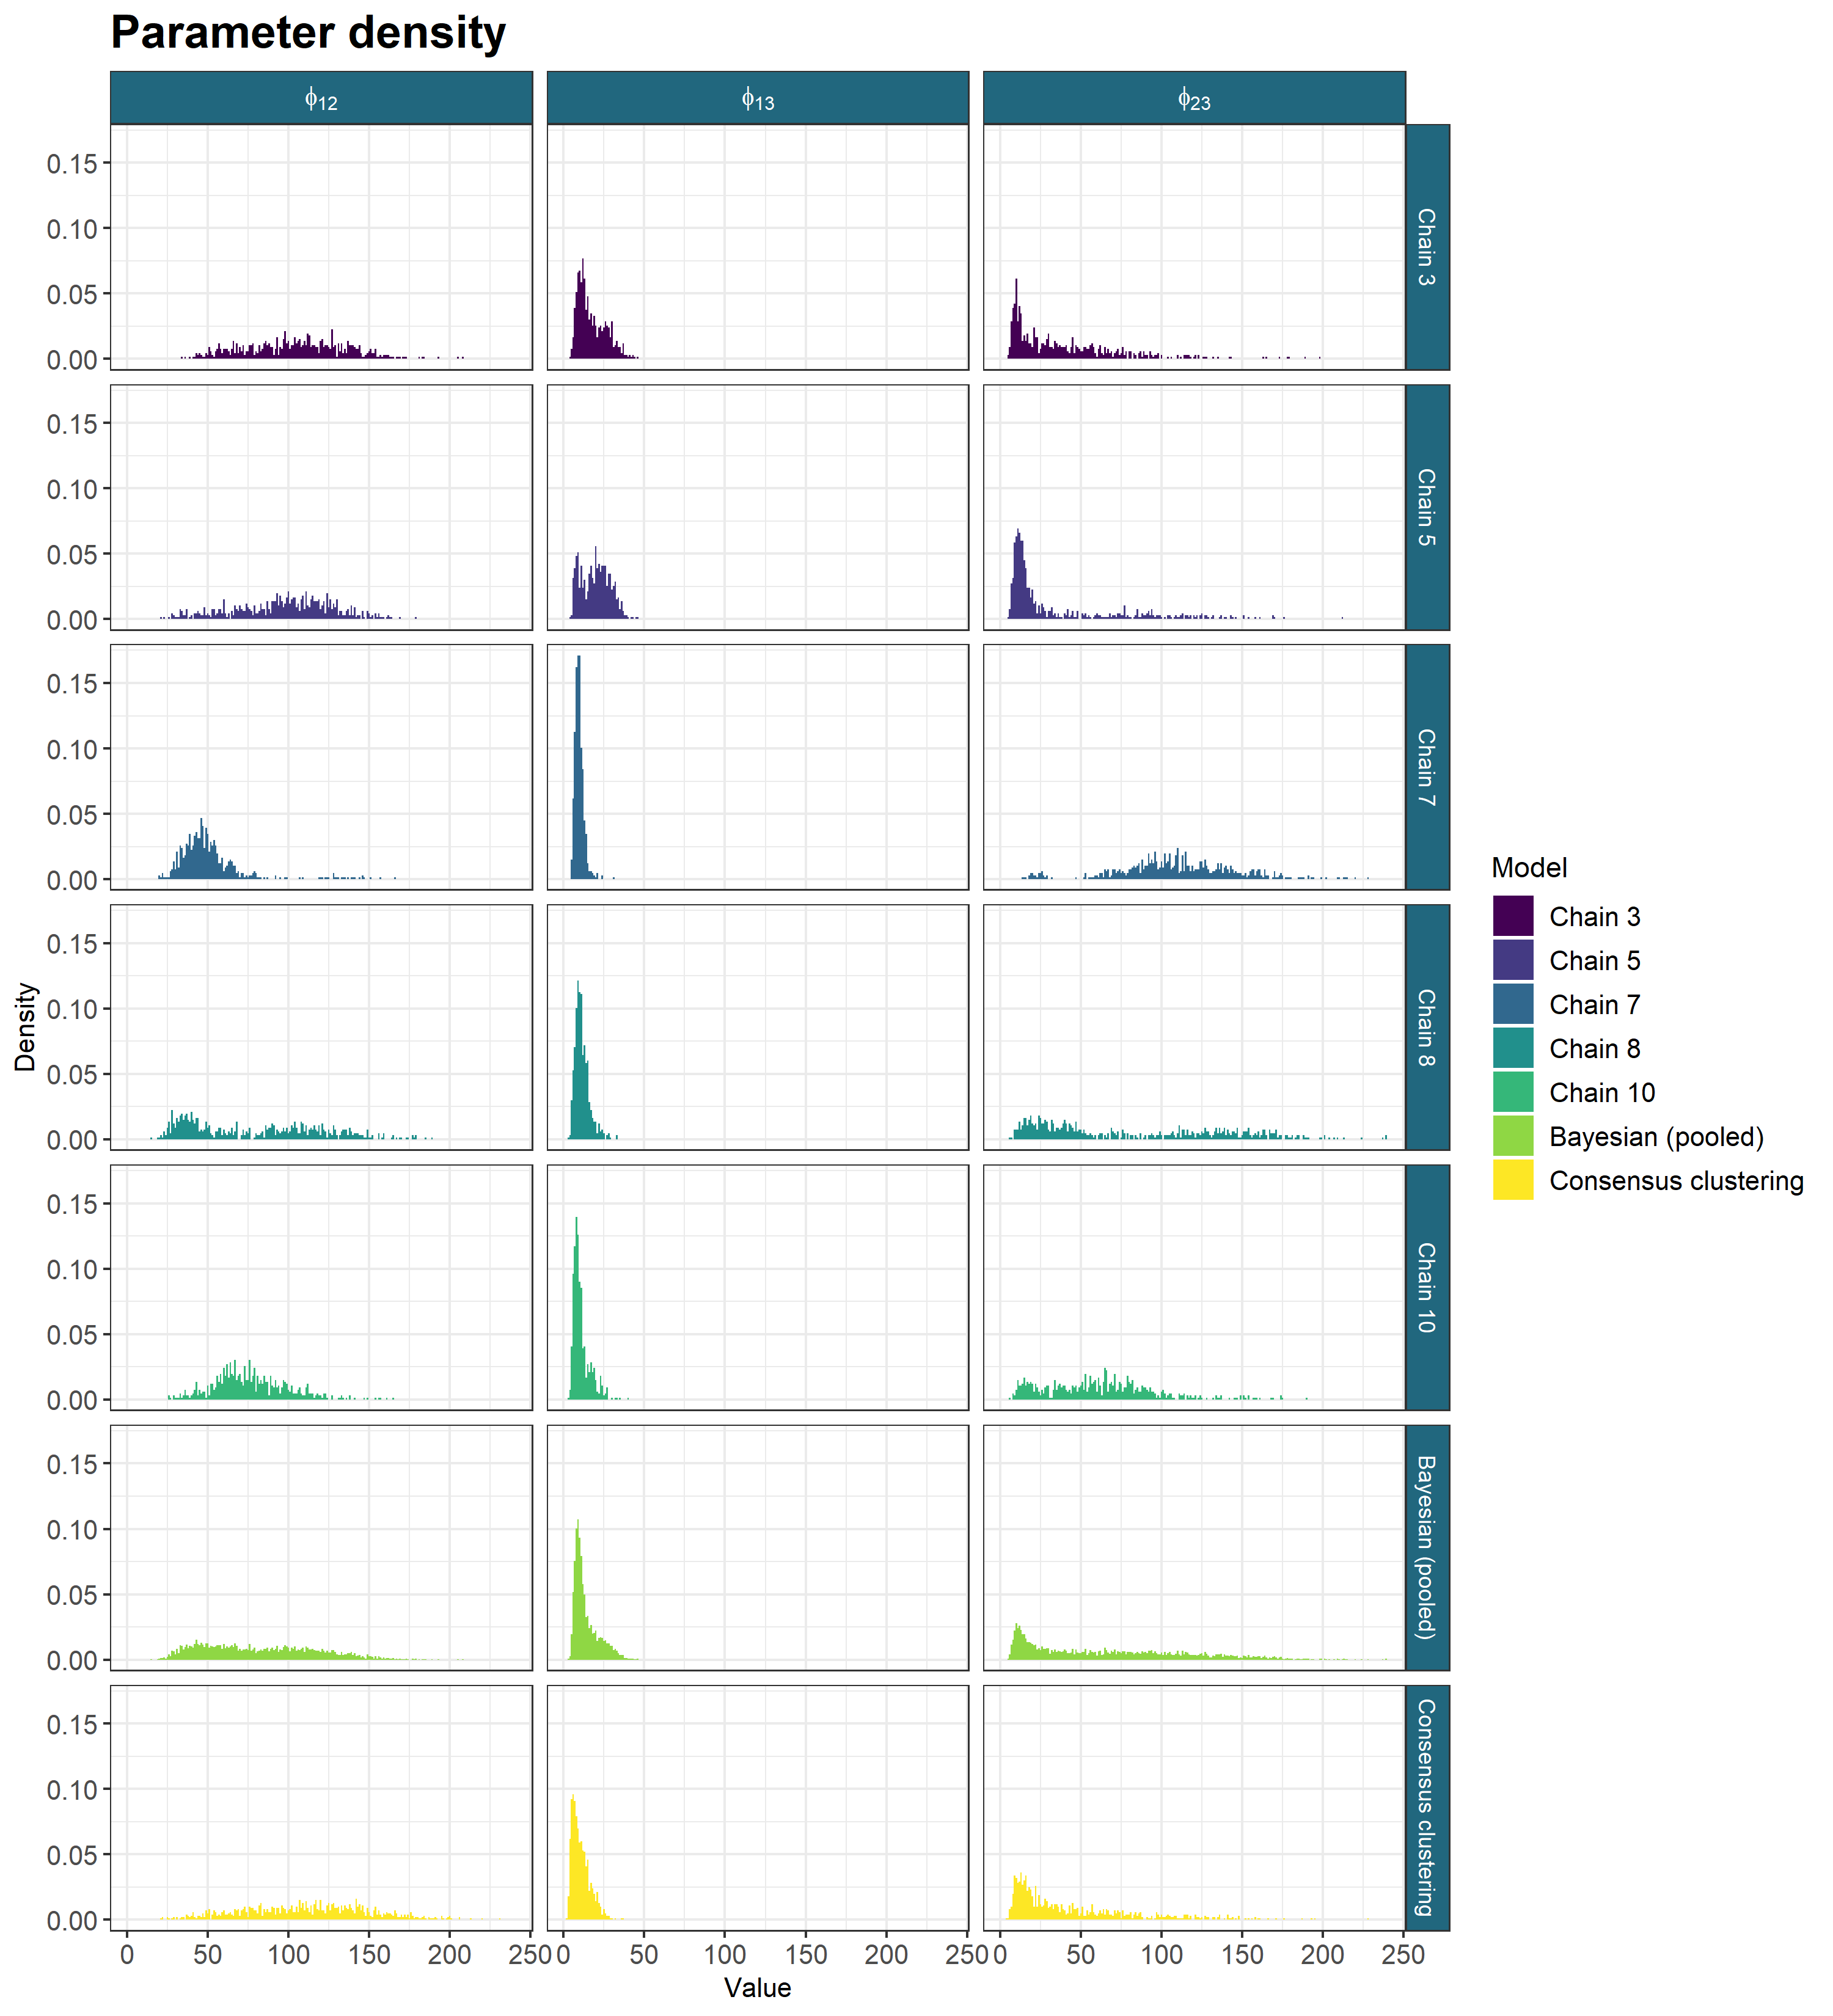
\includegraphics[scale=0.6]{./Images/Yeast/ComparisonDensities.png}
	\caption{The sampled values for the $\phi$ parameters from the long chains, their pooled samples and the consensus using 1000 chains of depth 10,001. The long chains display a variety of behaviours. Across chains there is no clear consensus on the nature of the posterior distribution. The samples from any single chain are not particularly close to the behaviour of the pooled samples across all three parameters. It is the Consensus clustering that most approaches this pooled behaviour.}
	\label{fig:densityComparison}
\end{figure}

%Evidence for this can also be seen in the coherent clusters of time series from the Timecourse dataset in figure \ref{fig:timecourseCCTimeSeries}.



\subsection{GO term over-representation} \label{sec:goTermOverRep}
To validate the predicted clusters we tested if they contained a higher concentration of specific Gene Ontology (GO) terms than would be expected by chance. We estimated clusterings from the PSMs of the chains kept from section \ref{sec:yeastBayesianAnalysis} visualised in figure \ref{fig:yeastPSMs} and the Consensus matrix of the largest ensemble run (i.e. $CC(10001, 1000)$) using the \texttt{maxpear} function from the R package \texttt{mcclust} \cite{fritsch2012mcclust} using default settings except for \texttt{k.max} which was set to 275 (the rounding down of $N/2$). To perform the GO term over-representation analysis we used the \texttt{Bioconductor} packages \texttt{clusterProfiler} \citep{yu2012clusterProfiler}, \texttt{biomaRt} \citep{durinck2009mapping} and the annotation package \texttt{org.Sc.sgd.db} \citep{carlson2014org}.

We conditioned the test on the background set of the 551 yeast genes in the data. The gene labelled YIL167W was not found in the annotation database and was dropped from the analysis leaving a background universe of 550 genes. A hypergeometric test was used to check if the number of genes associated with specific GO terms within a cluster was greater than expected by random chance. We corrected the $p$-values using the Benjamini-Hochberg correction \citep{benjamini1995controlling} and defined significance by a threshold of 0.01. We plotted the over-represented GO terms for the different clusterings within each dataset using the three different ontologies of ``Molecular function" (\textbf{MF}), ``Biological process" (\textbf{BP}) and ``Cellular component" (\textbf{CC}) (figures \ref{fig:yeastGOMF}, \ref{fig:yeastGOBP} and \ref{fig:yeastGOCC} respectively). 

We find that the Consensus clustering finds terms common to all of the long chains. It also finds some terms with low $p$-values common to a majority of chains (such as DNA helicase activity in the MF ontology for the Timecourse dataset) and a small number of GO terms unique to itself. These terms that no long chain find are normally related to other terms already over-represented within either the Consensus clustering or a number of the long chains. For example, the transmembrane transporter activity and transporter activity terms uncovered by the ensemble in the Timecourse dataset are related to terms found across 3 of the chains and by Consensus clustering (specifically transferase activity and phosphotransferase). 
%We believe that the clustering provided by Consensus clustering of MDI results in a meaningful clustering that can uncover


Furthermore, we also note that the Bayesian chains have very significant disagreements between eachother; there is no consensus on the results with many terms enriched in one or two chains (see the behaviour in any ontology for the ChIP-chip and PPI datasets). We argue that the final partition from Consensus clustering is more consistent than any of the individual long chains, agreeing where the chains agree and providing sensible differences to any given chain. As the chains are not converged and there is no clear overlap, a full analysis would be difficult to defend using any one of these long chains. 

ASIDE: I THINK I NEED A STATEMENT LIKE THIS, BUT FEEL IT IS A LITTLE HEAVY-HANDED

We believe that Consensus clustering does offer a solution to problems preventing the use of complex models such as MDI in their currently implemented forms, finding meaningful structure in a reproducible analysis.

%PPI MF GO:
%There is much disagreement between the Bayesian chains; more so in this case with no terms found in all 5 chains. This is the dataset with the most disagreement between chains in the PSMs (as seen in figure \ref{fig:yeastPSMs}).
%
%ChIP-chip MF GO:
%there is more consistency across chains, but there is still significant disagreement. The Consensus clustering finds largely terms that are common to several chains. Some terms are unique to the Consensus clustering, for example \emph{DNA binding} and \emph{nucleic acid binding} emerge in the Consensus clustering but no Bayesian chain, but this terms have overlap in their associated genes and thus evidence for one suggests the other. Furthermore, 3 clusters in chain 10 from the Bayesian analysis does have terms associated with binding over-represented in three clusters and chains 3 and 5 have many different types of binding emerging. Thus the binding terms found by the Consensus clustering are partially supported in the long chains. The other two terms unique to Consensus clustering, transmembrane transporter activity and transporter activity, are both related to each other. Transferase activity and phosphotransferase, two terms found by both Consensus clustering and three of the Bayesian chains, are associated with transporting molecules within the cell and across the cell membrane. Thus the emergence of additional terms associated with transportation are not surprising, particularly as those unique to Consensus clustering have small $p$-values.

%\begin{figure}
%	\centering
%	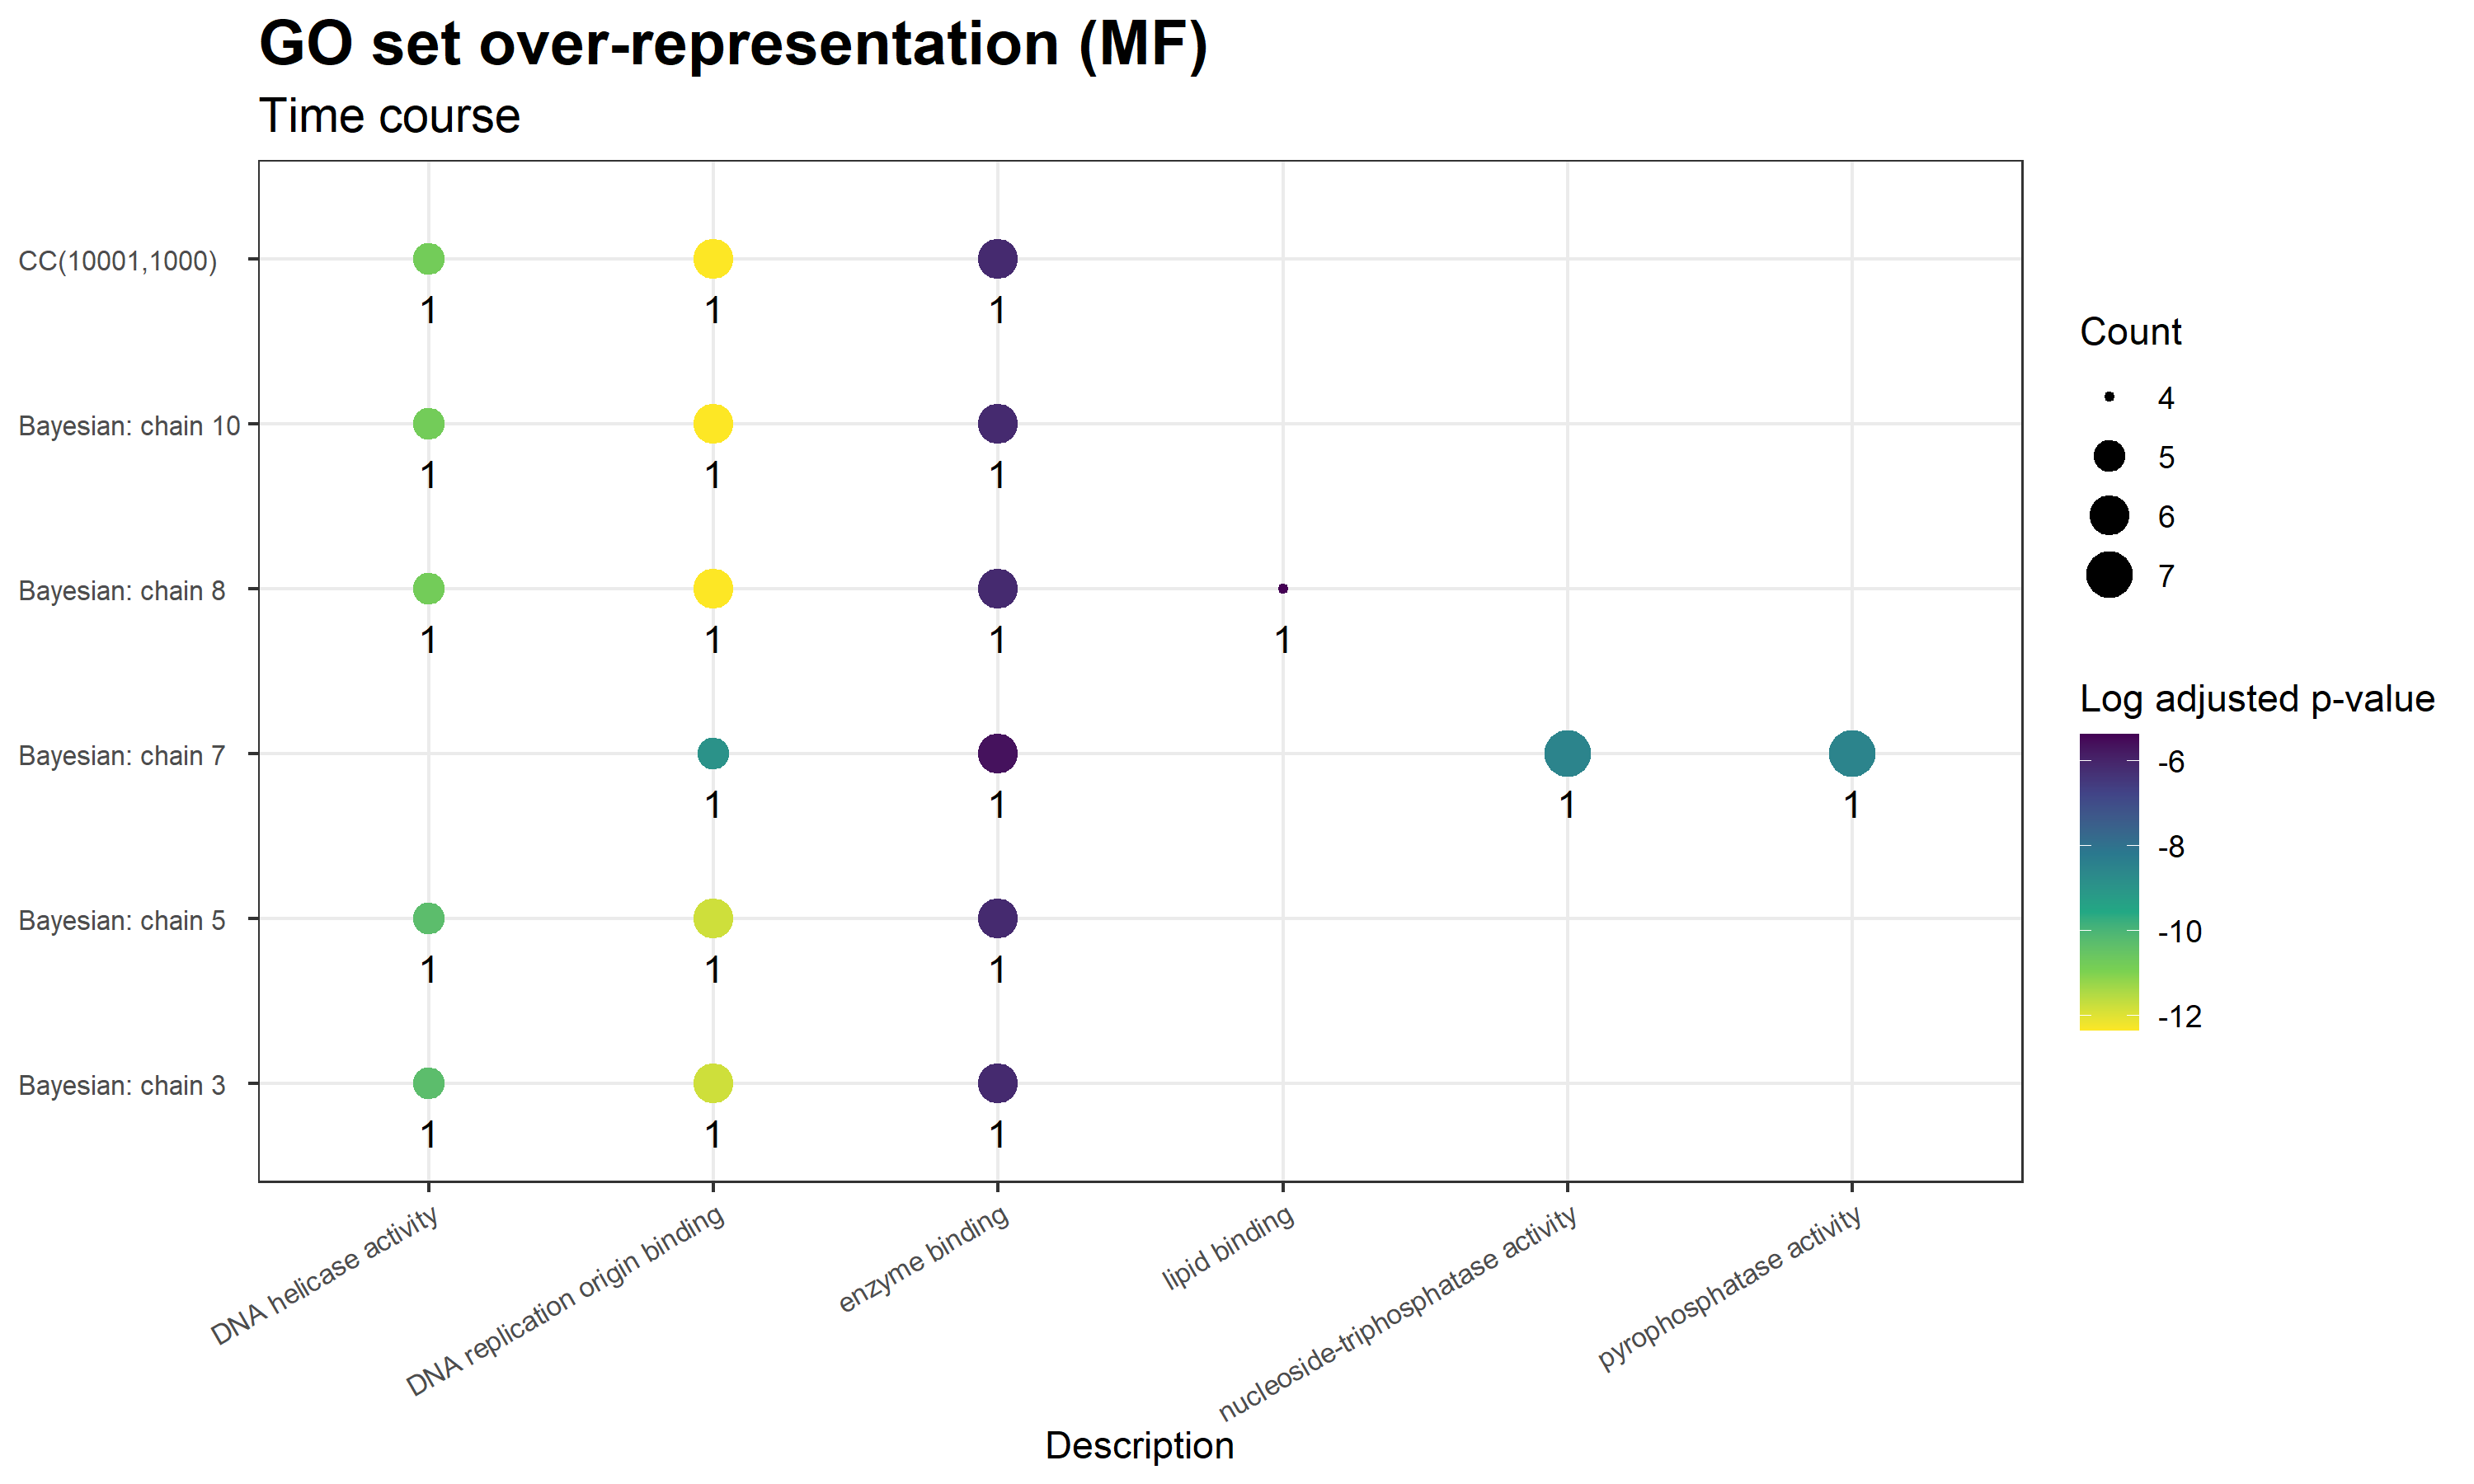
\includegraphics[scale=0.5]{./Images/Yeast/TimecoursegoEnrichmentCompMF.png}
%	\caption{GO enrichment for the Molecular function ontology in the Timecourse dataset. Each dot corresponds to a GO term that was over-represented in at least one cluster in the analysis, with colour corresponding to the adjusted $p$-value and size to the number items associated with that term in the given cluster. The number below each dot is the number of clusters from the analysis that were enriched for the term. Terms common to all chains are found also by Consensus clustering. Many terms are found only in a subset of chains. Except for DNA helicase activity, which has smaller associated $p$-values, no GO term not found in all 5 chains is over-represented in the Consensus clustering.}
%	\label{fig:timecourseGOMF}
%\end{figure}
%
%\begin{figure}
%	\centering
%	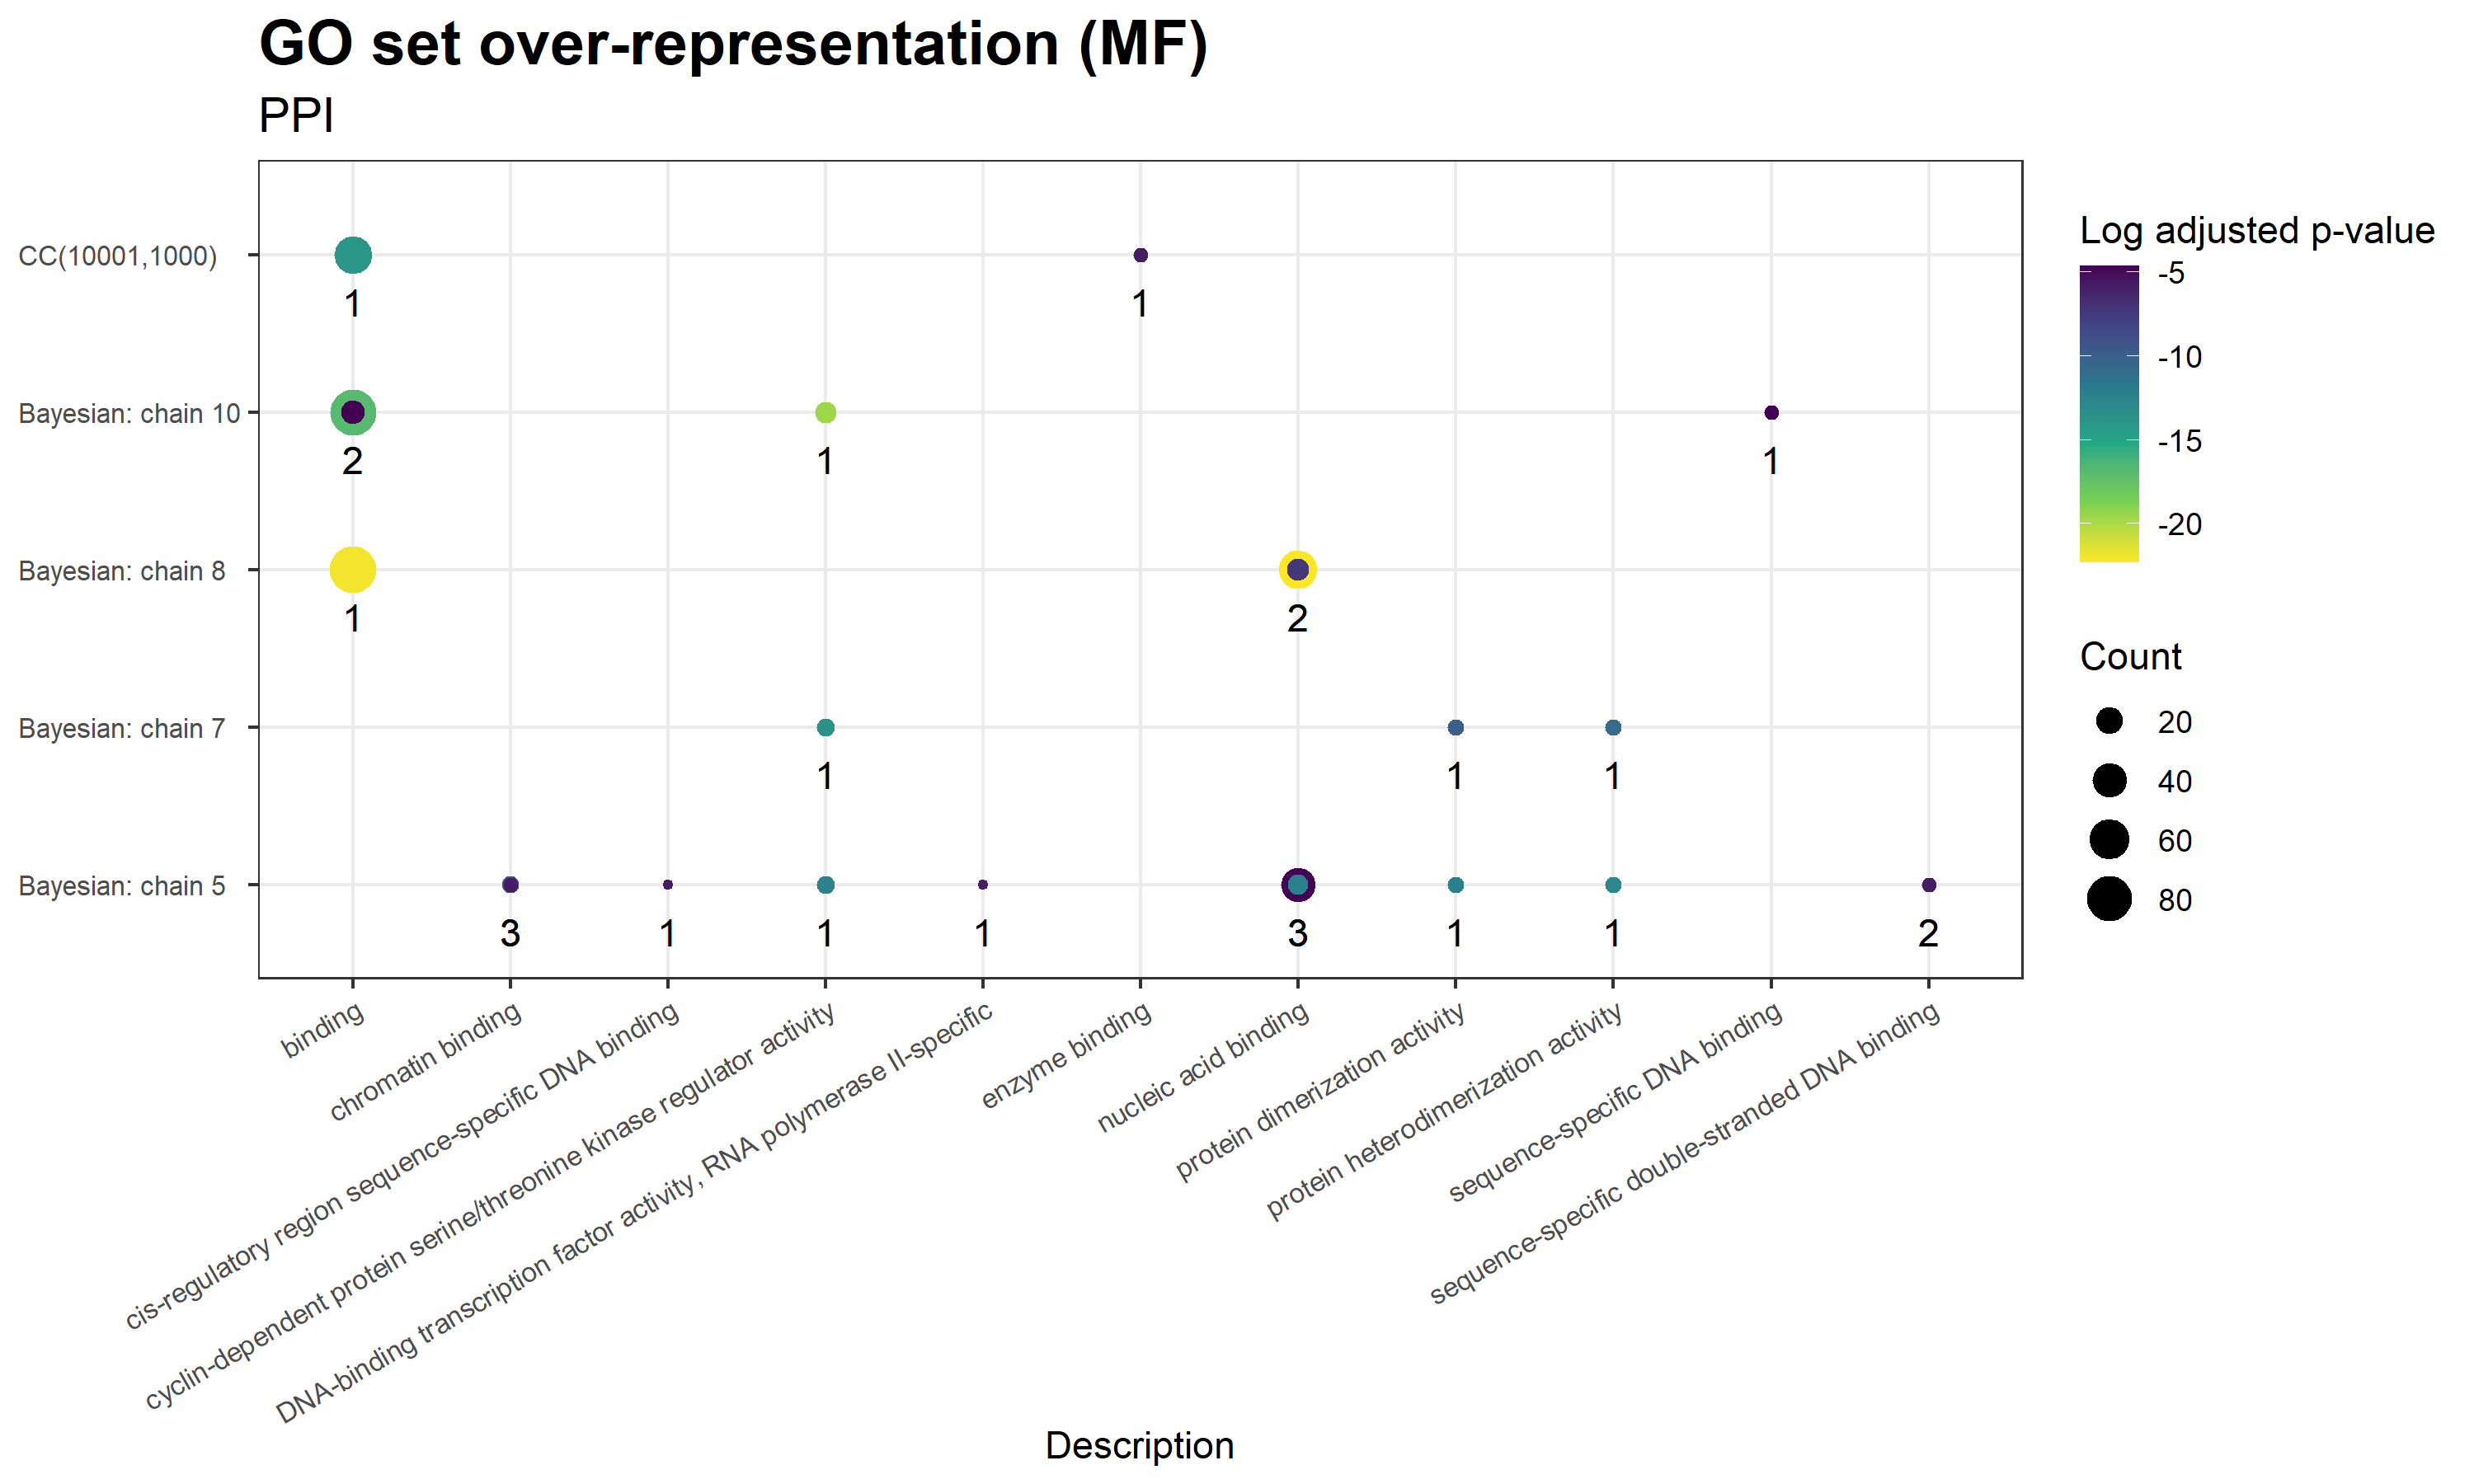
\includegraphics[scale=0.5]{./Images/Yeast/PPIgoEnrichmentCompMF.png}
%	\caption{GO enrichment for the Molecular function ontology in the PPI dataset. Each dot corresponds to a GO term that was over-represented in at least one cluster in the analysis, with colour corresponding to the adjusted $p$-value and size to the number items associated with that term in the given cluster. The number below each dot is the number of clusters from the analysis that were enriched for the term. Similar to figure \ref{fig:timecourseGOMF}, there is much disagreement between the Bayesian chains; more so in this case with no terms found in all 5 chains. This is the dataset with the most disagreement between chains in the PSMs (as seen in figure \ref{fig:yeastPSMs}).}
%	\label{fig:ppiGOMF}
%\end{figure}
%
%\begin{figure}
%	\centering
%	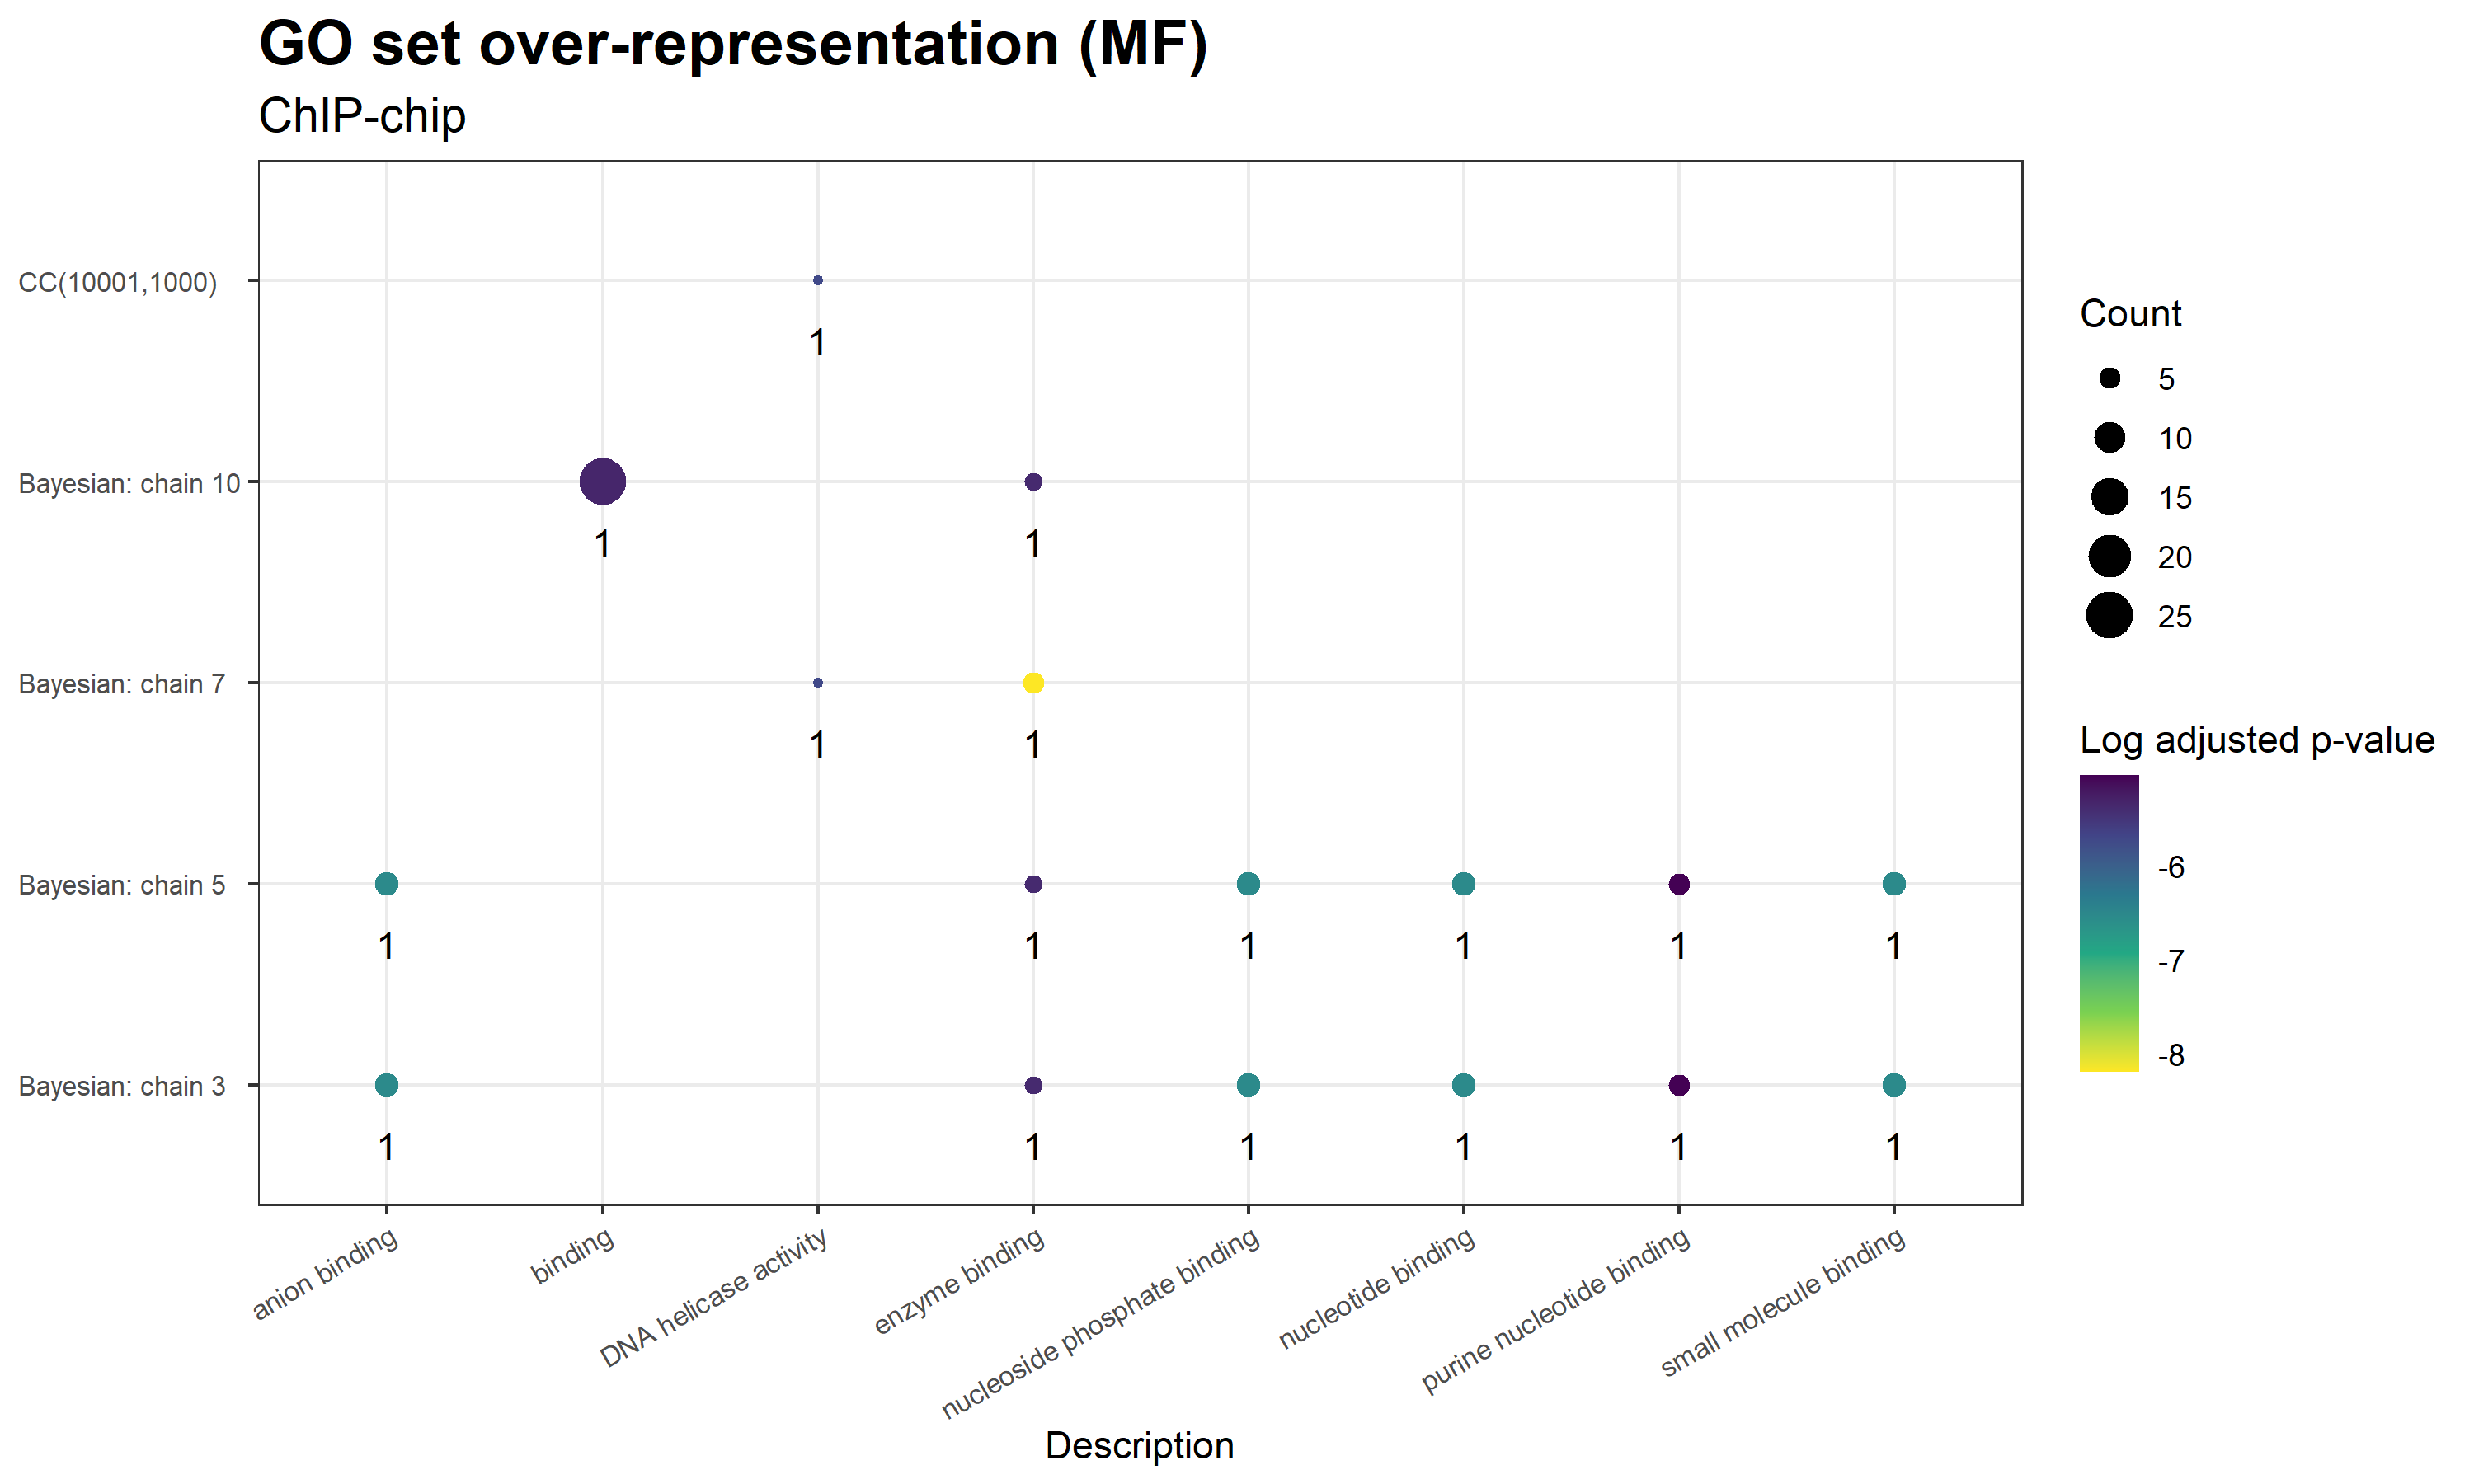
\includegraphics[scale=0.5]{./Images/Yeast/ChIP-chipgoEnrichmentCompMF.png}
%	\caption{GO enrichment for the Molecular function ontology in the ChIP-chip dataset. Each dot corresponds to a GO term that was over-represented in at least one cluster in the analysis, with colour corresponding to the adjusted $p$-value and size to the number items associated with that term in the given cluster. The number below each dot is the number of clusters from the analysis that were enriched for the term. Here there is more consistency across chains, but there is still significant disagreement. The Consensus clustering finds largely terms that are common to several chains. Some terms are unique to the Consensus clustering, for example \emph{DNA binding} and \emph{nucleic acid binding} emerge in the Consensus clustering but no Bayesian chain, but this terms have overlap in their associated genes and thus evidence for one suggests the other. Furthermore, 3 clusters in chain 10 from the Bayesian analysis does have terms associated with binding over-represented in three clusters and chains 3 and 5 have many different types of binding emerging. Thus the binding terms found by the Consensus clustering are partially supported in the long chains. The other two terms unique to Consensus clustering, transmembrane transporter activity and transporter activity, are both related to each other. Transferase activity and phosphotransferase, two terms found by both Consensus clustering and three of the Bayesian chains, are associated with transporting molecules within the cell and across the cell membrane. Thus the emergence of additional terms associated with transportation are not surprising, particularly as those unique to Consensus clustering have small $p$-values.}
%	\label{fig:chipchipGOMF}
%\end{figure}

%\begin{figure}
%	\centering
%	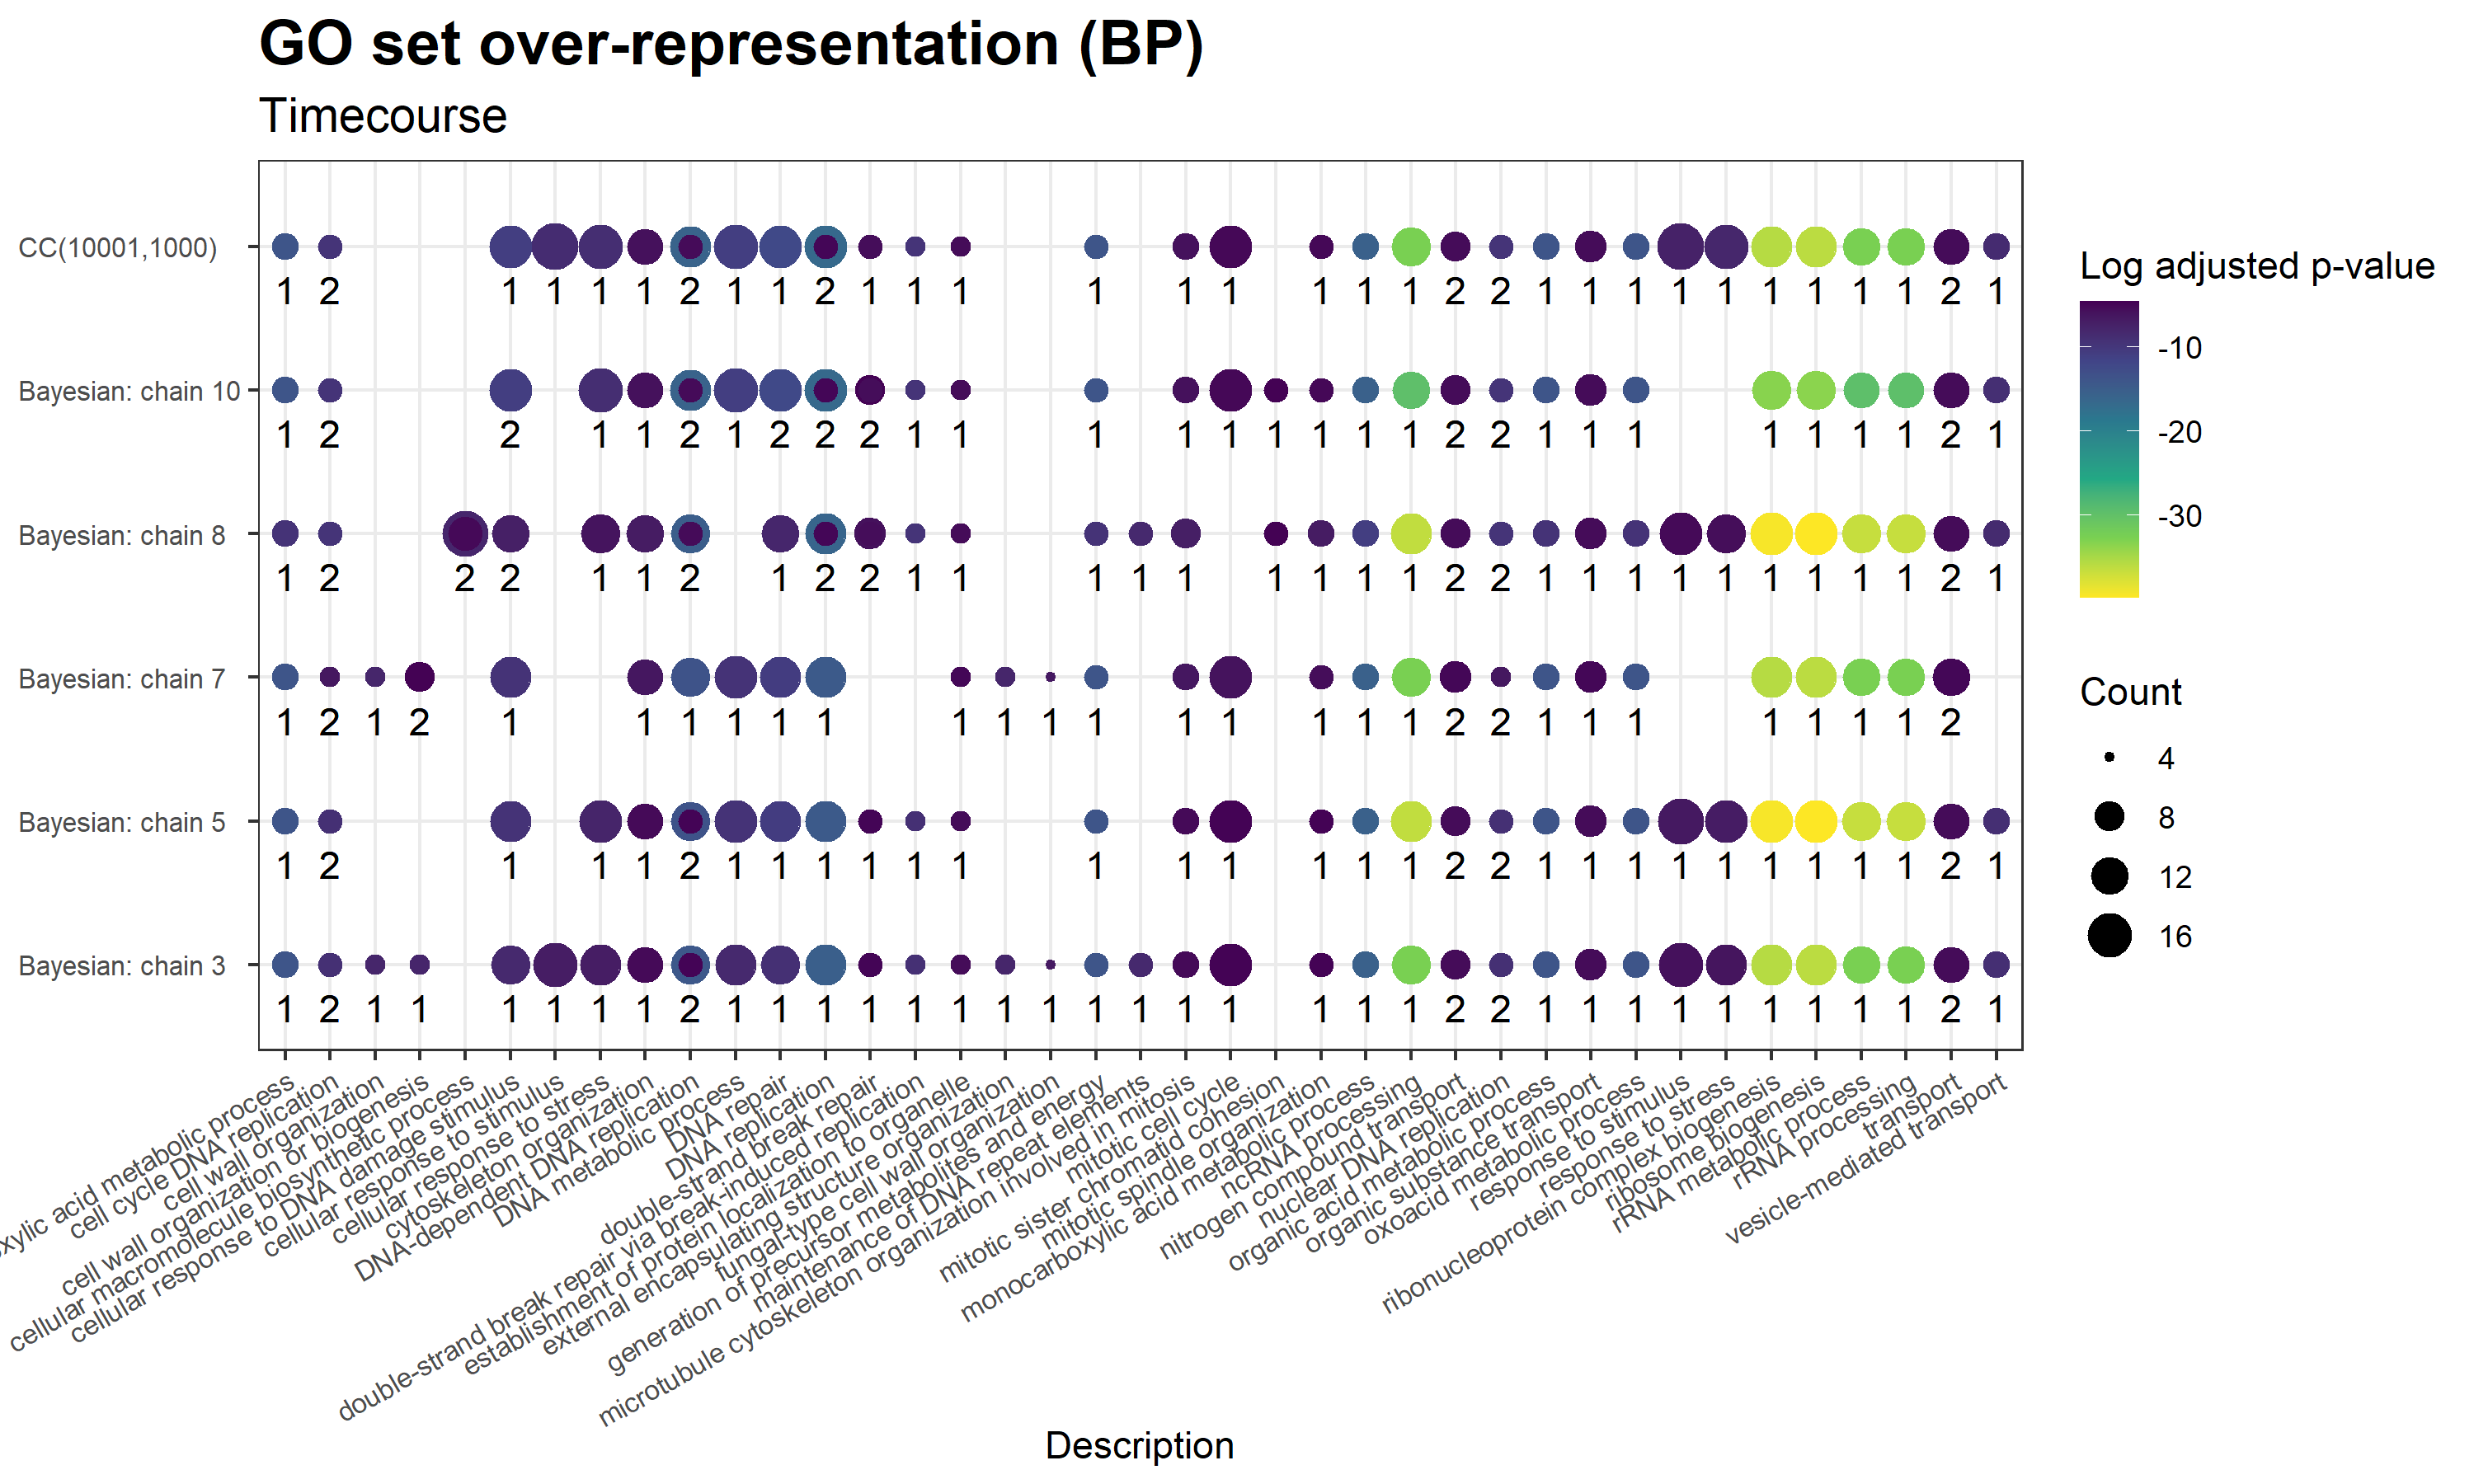
\includegraphics[scale=0.5]{./Images/Yeast/TimecoursegoEnrichmentCompBP.png}
%	\caption{GO enrichment for the Biological process ontology in the Timecourse dataset. Each dot corresponds to a GO term that was over-represented in at least one cluster in the analysis, with colour corresponding to the adjusted $p$-value and size to the number items associated with that term in the given cluster. The number below each dot is the number of clusters from the analysis that were enriched for the term.}
%	\label{fig:timecourseGOBP}
%\end{figure}
%
%\begin{figure}
%	\centering
%	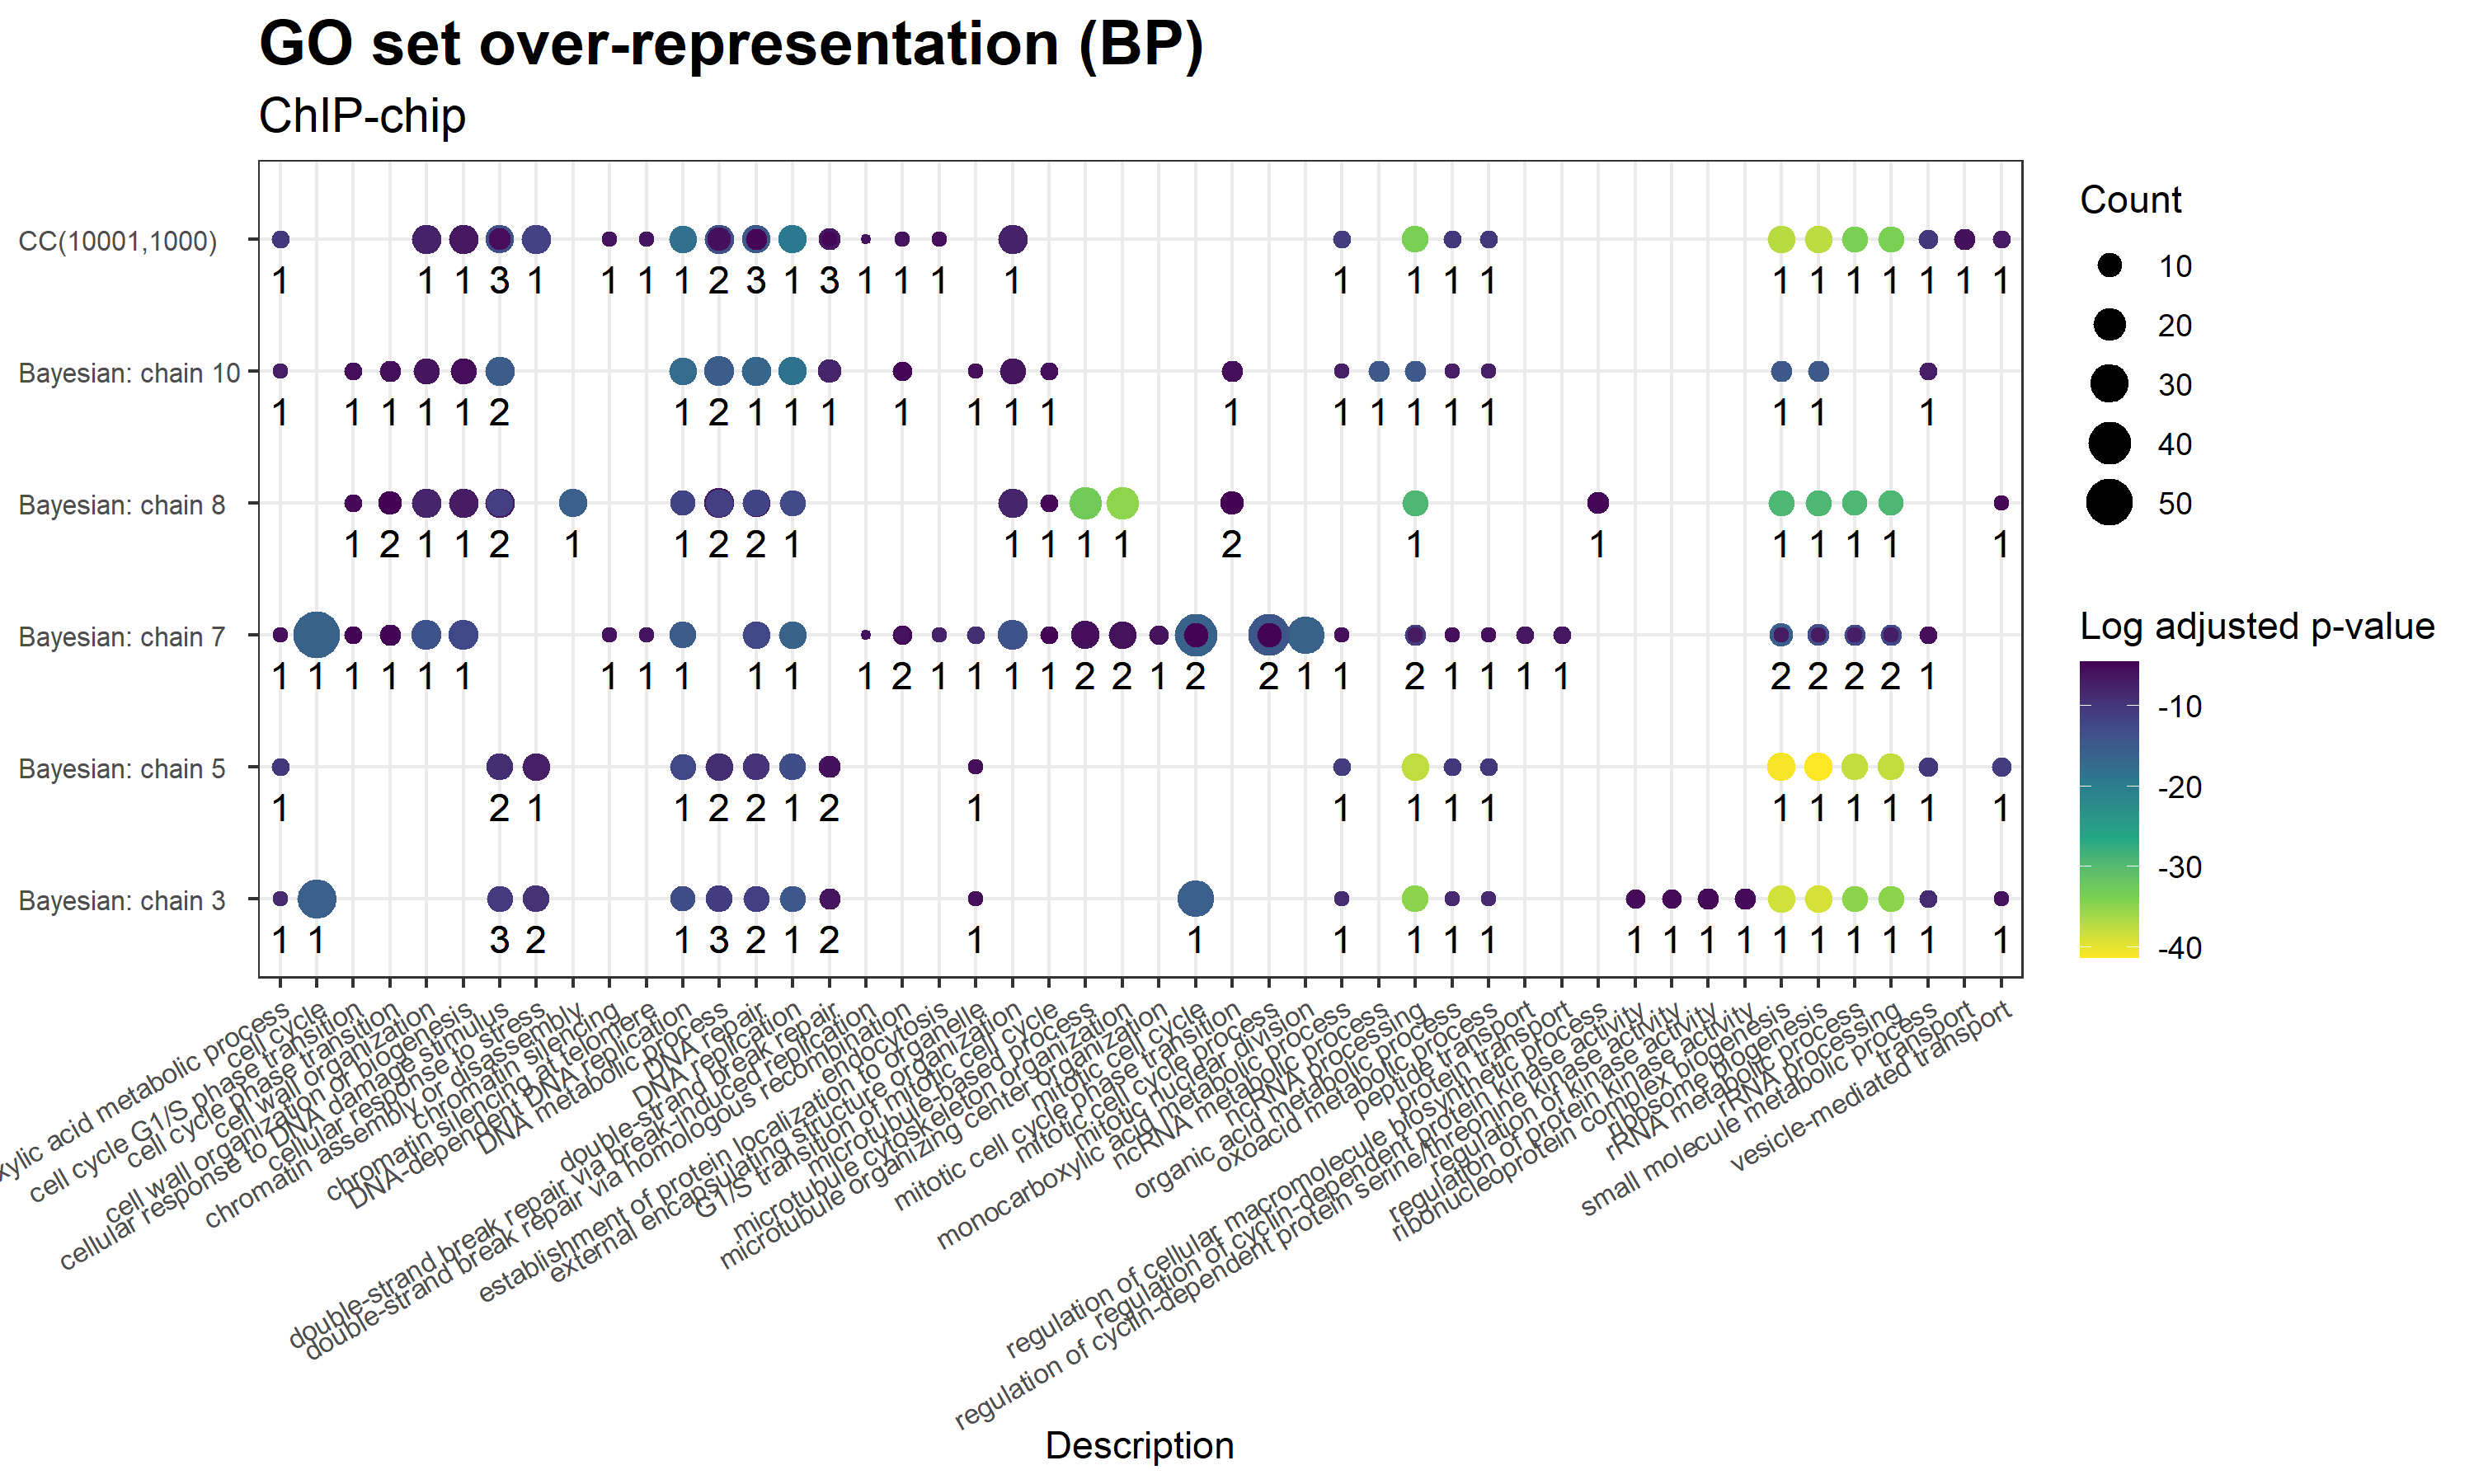
\includegraphics[scale=0.5]{./Images/Yeast/ChIP-chipgoEnrichmentCompBP.png}
%	\caption{GO enrichment for the Biological process ontology in the ChIP-chip dataset. Each dot corresponds to a GO term that was over-represented in at least one cluster in the analysis, with colour corresponding to the adjusted $p$-value and size to the number items associated with that term in the given cluster. The number below each dot is the number of clusters from the analysis that were enriched for the term.}
%	\label{fig:chipchipGOBP}
%\end{figure}
%
%\begin{figure}
%	\centering
%	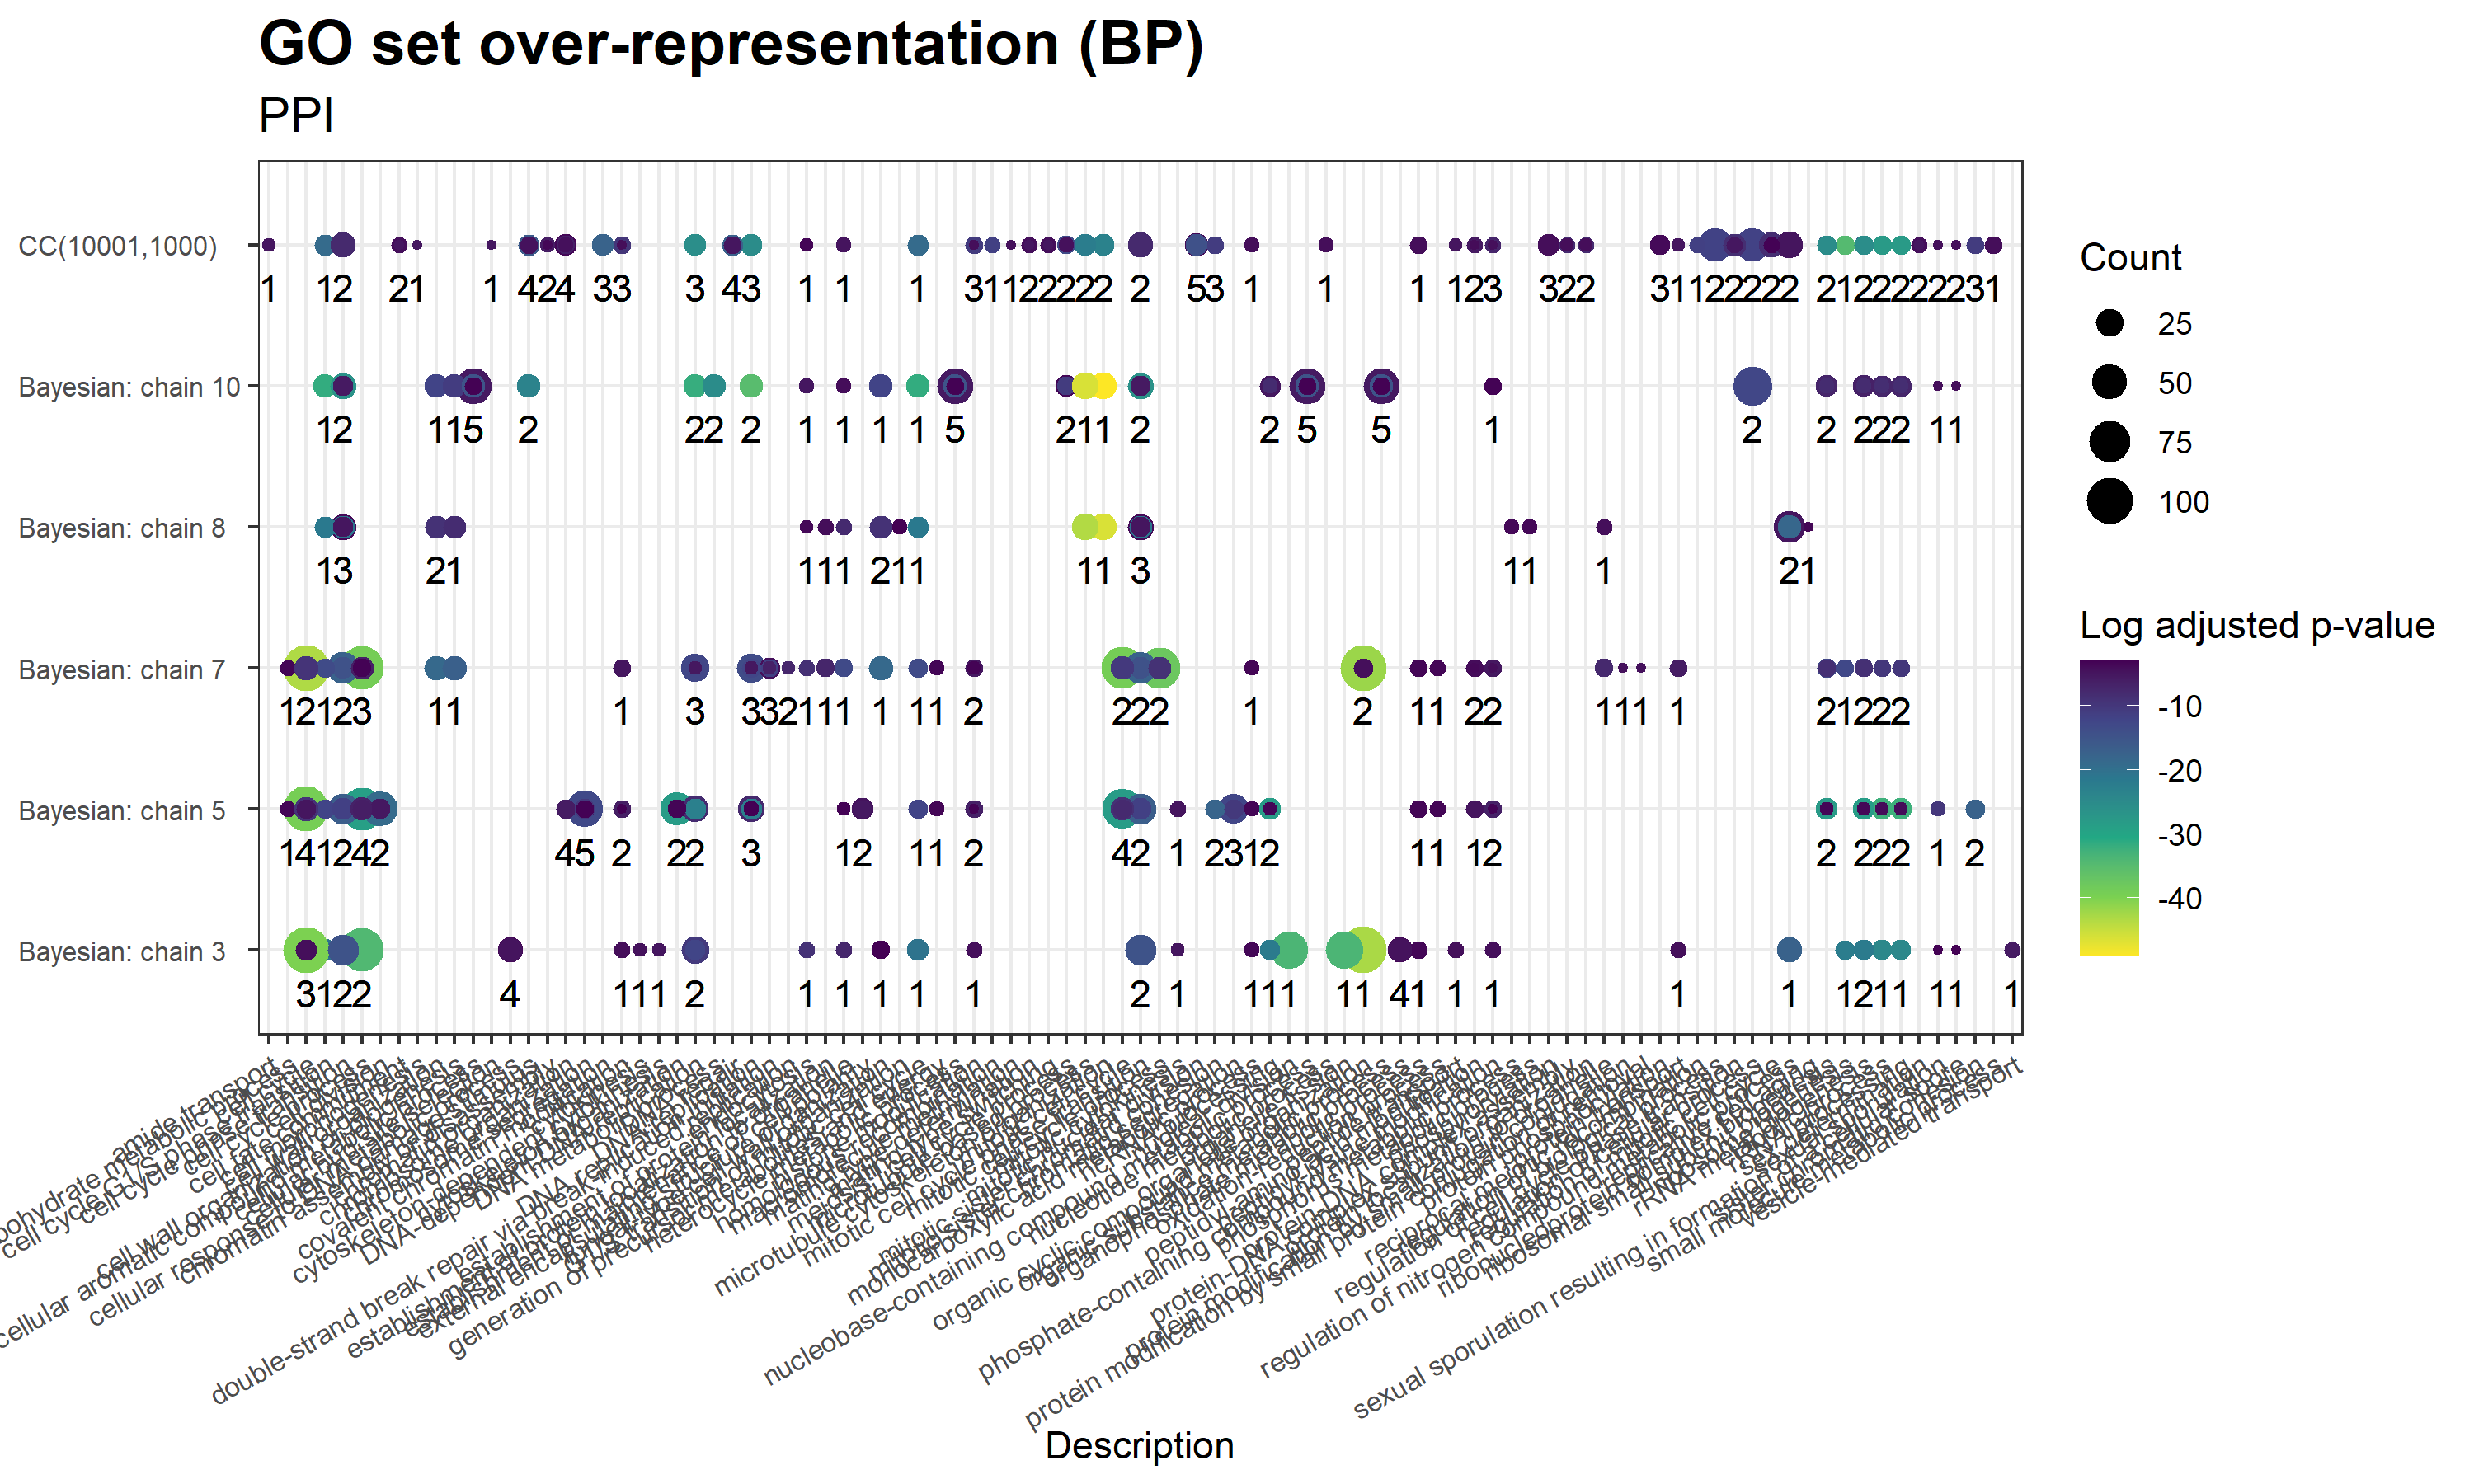
\includegraphics[scale=0.5]{./Images/Yeast/PPIgoEnrichmentCompBP.png}
%	\caption{GO enrichment for the Biological process ontology in the PPI dataset. Each dot corresponds to a GO term that was over-represented in at least one cluster in the analysis, with colour corresponding to the adjusted $p$-value and size to the number items associated with that term in the given cluster. The number below each dot is the number of clusters from the analysis that were enriched for the term.}
%	\label{fig:ppiGOBP}
%\end{figure}
%
%\begin{figure}
%	\centering
%	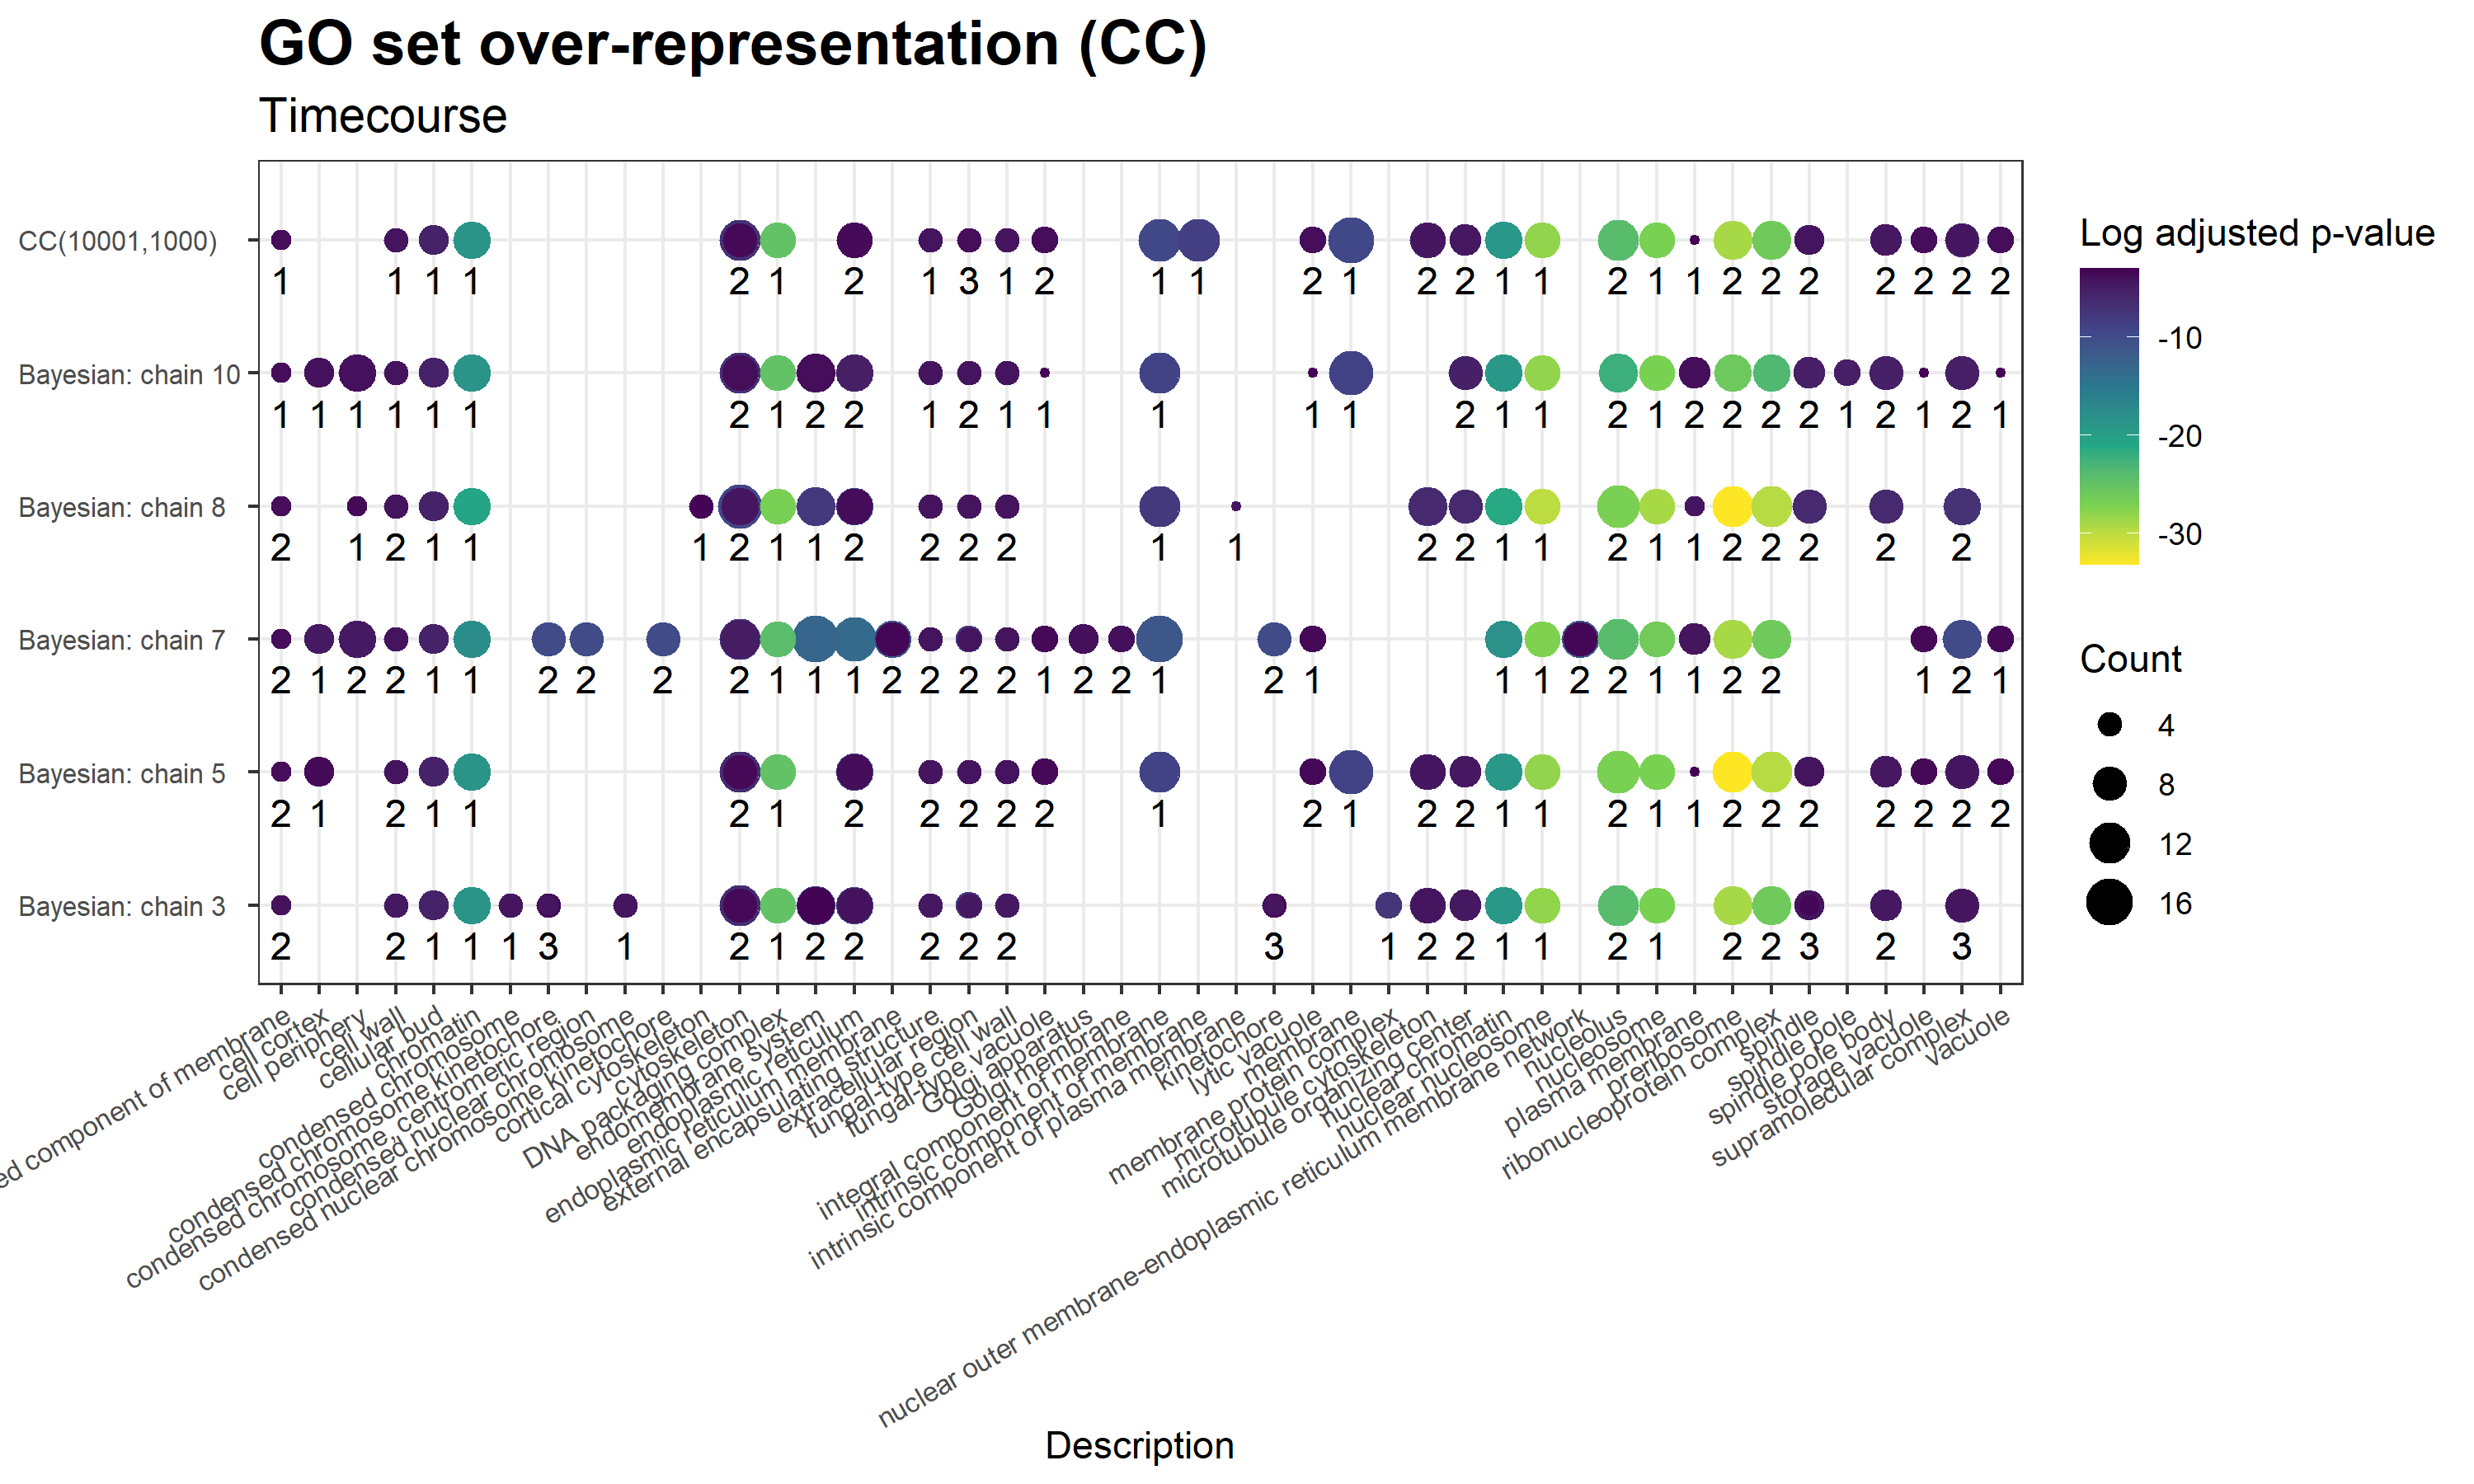
\includegraphics[scale=0.5]{./Images/Yeast/TimecoursegoEnrichmentCompCC.png}
%	\caption{GO enrichment for the Cellular component ontology in the Timecourse dataset. Each dot corresponds to a GO term that was over-represented in at least one cluster in the analysis, with colour corresponding to the adjusted $p$-value and size to the number items associated with that term in the given cluster. The number below each dot is the number of clusters from the analysis that were enriched for the term.}
%	\label{fig:timecourseGOCC}
%\end{figure}
%
%\begin{figure}
%	\centering
%	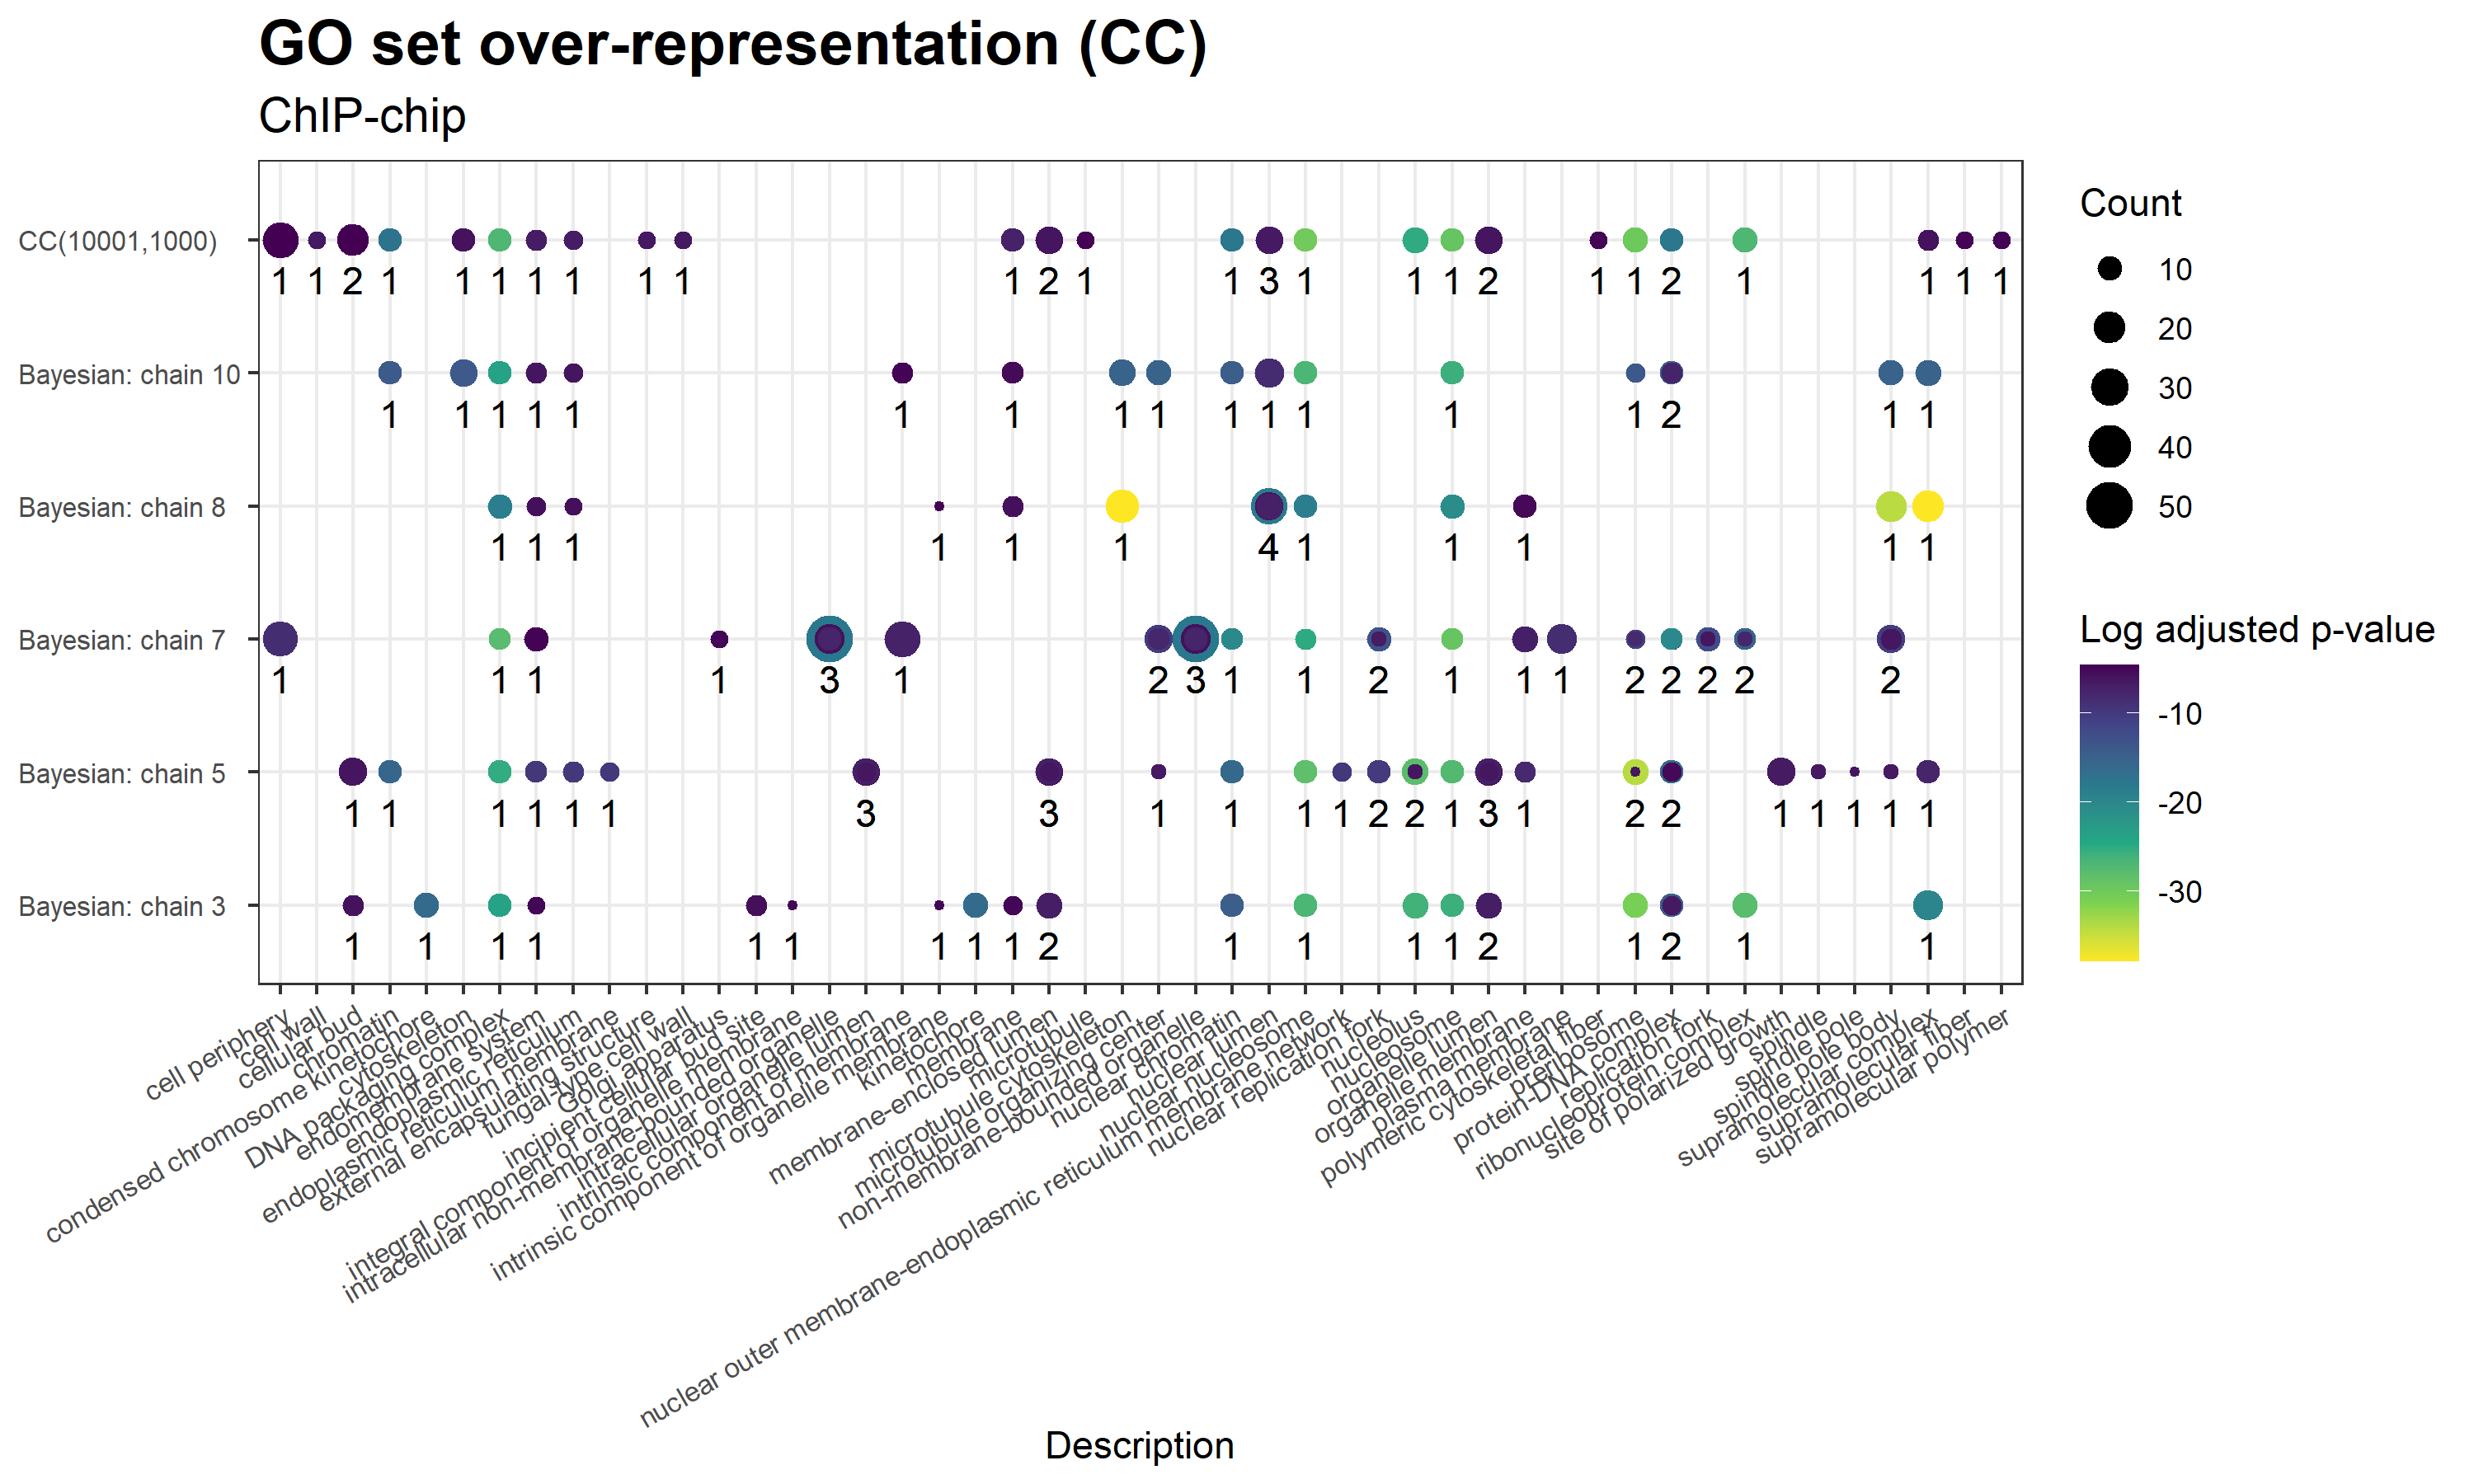
\includegraphics[scale=0.5]{./Images/Yeast/ChIP-chipgoEnrichmentCompCC.png}
%	\caption{GO enrichment for the Cellular component ontology in the ChIP-chip dataset. Each dot corresponds to a GO term that was over-represented in at least one cluster in the analysis, with colour corresponding to the adjusted $p$-value and size to the number items associated with that term in the given cluster. The number below each dot is the number of clusters from the analysis that were enriched for the term.}
%	\label{fig:chipchipGOCC}
%\end{figure}
%
%\begin{figure}
%	\centering
%	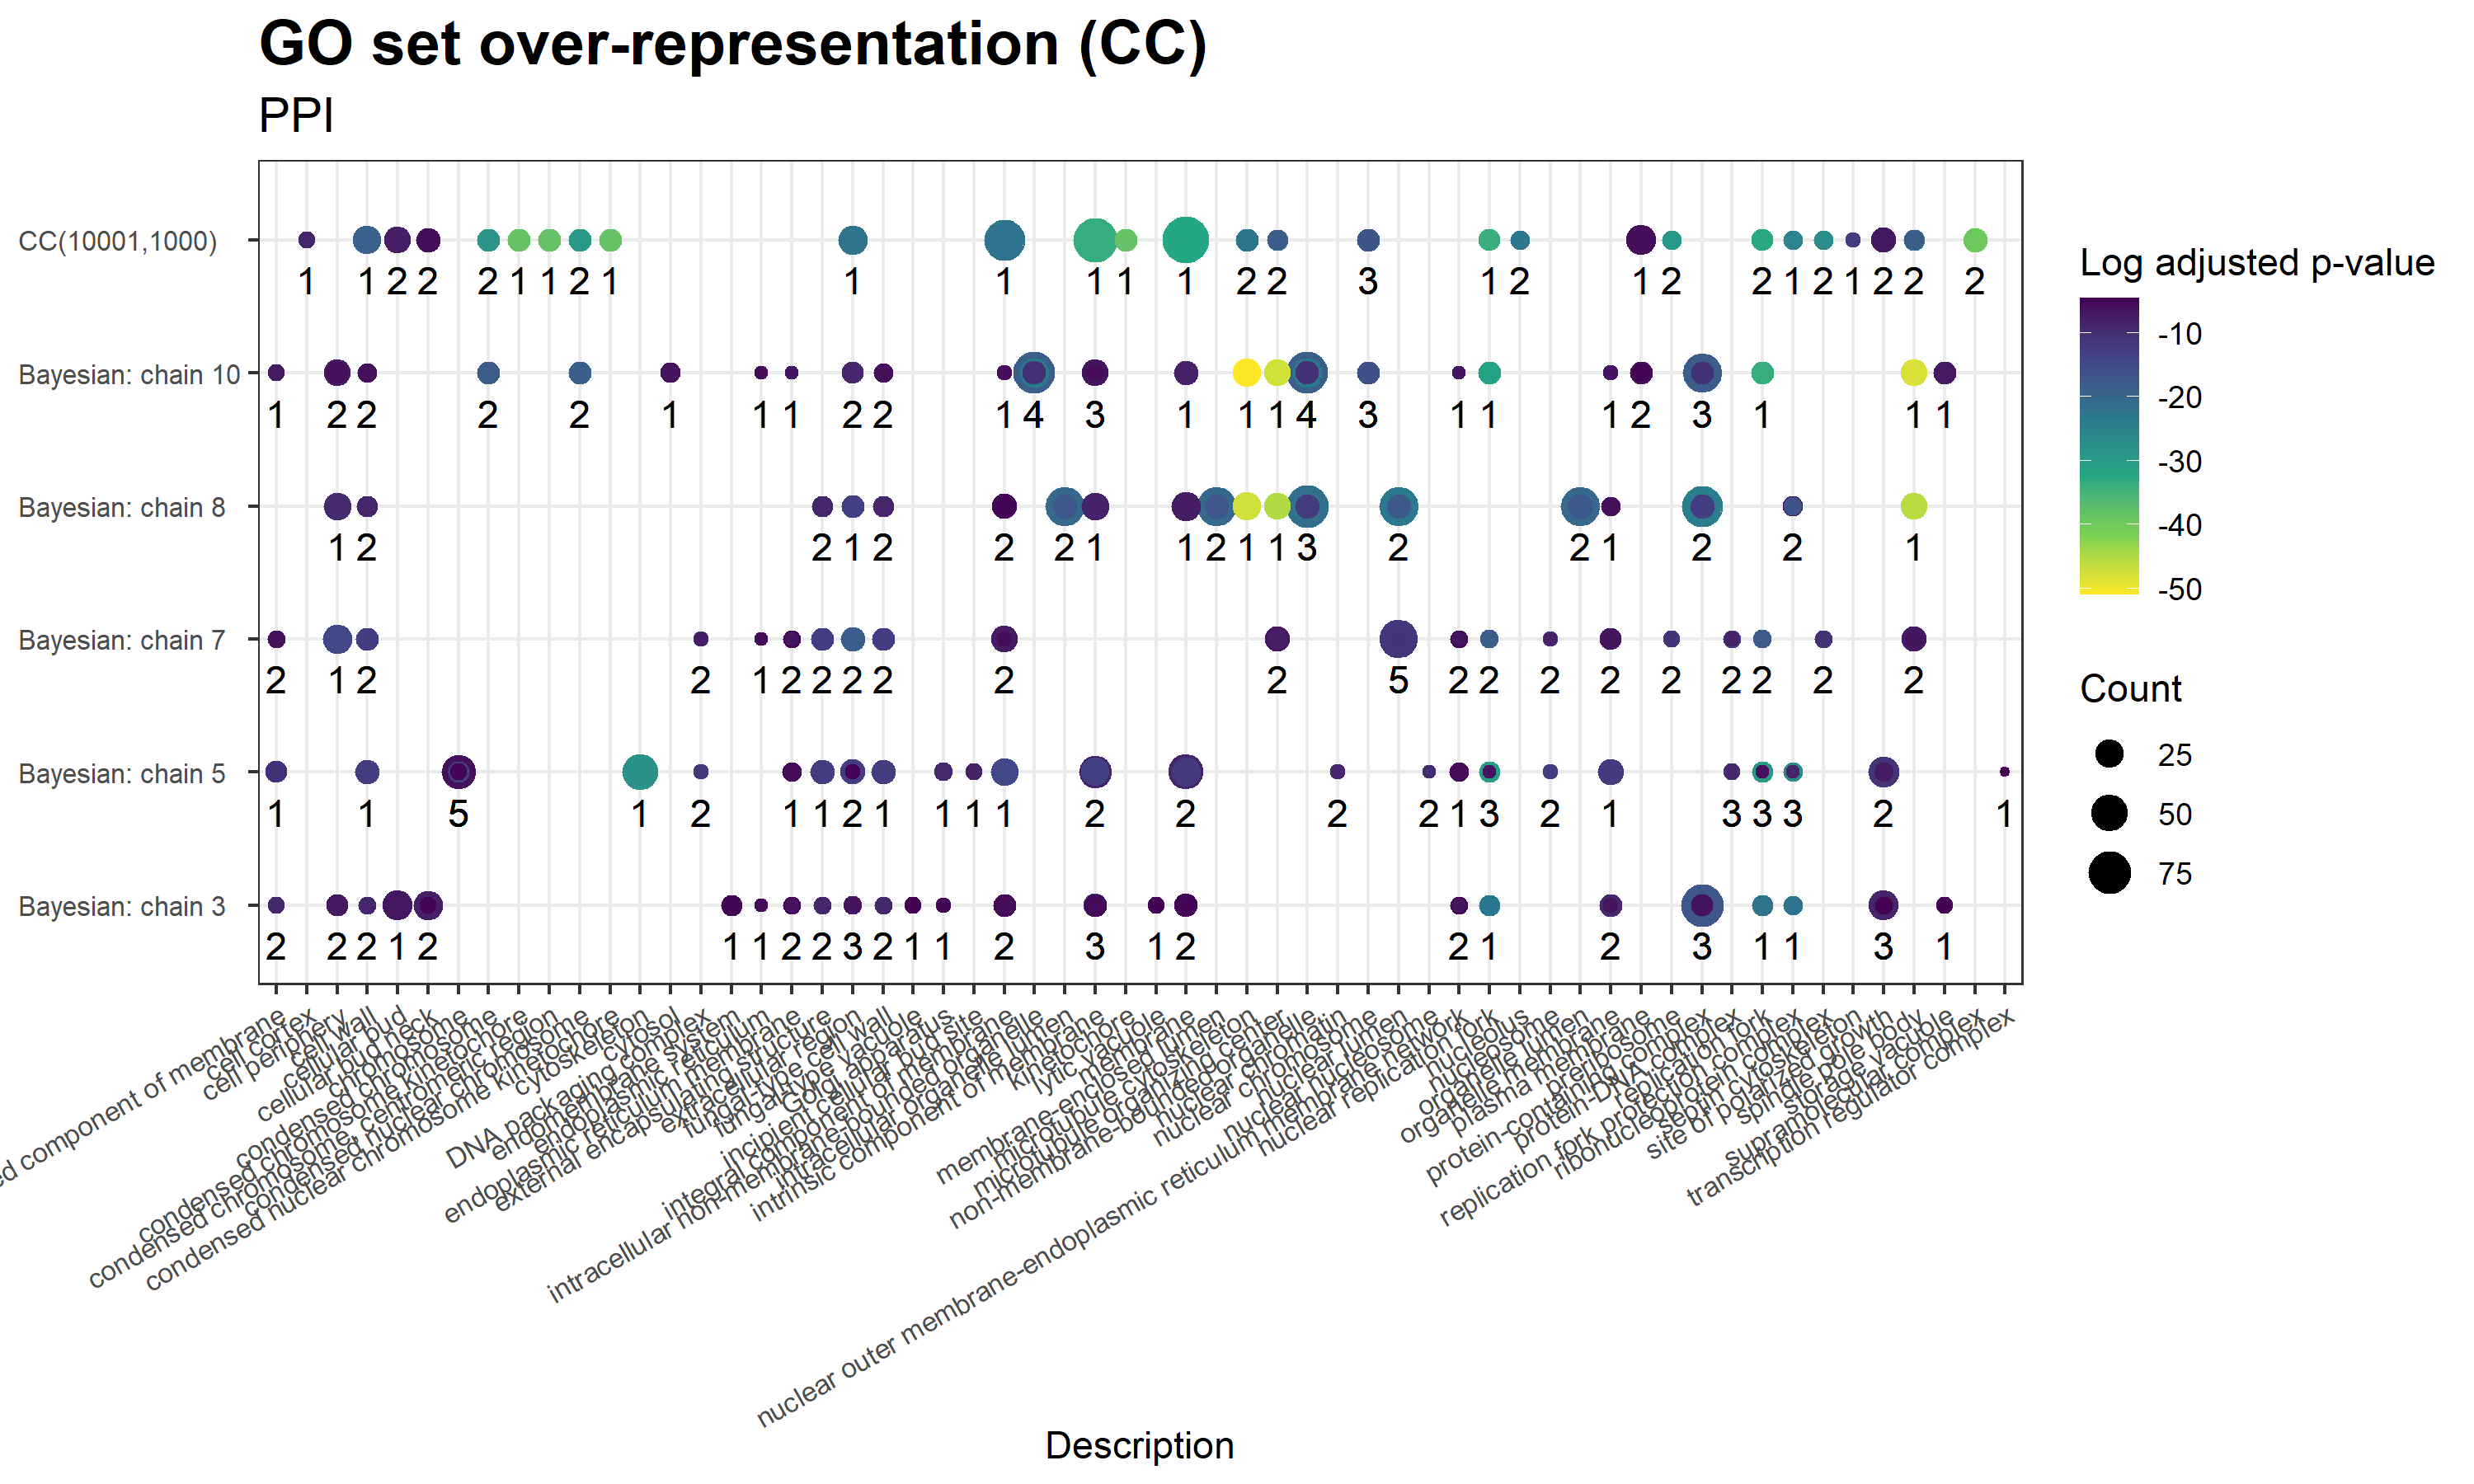
\includegraphics[scale=0.5]{./Images/Yeast/PPIgoEnrichmentCompCC.png}
%	\caption{GO enrichment for the Cellular component ontology in the PPI dataset. Each dot corresponds to a GO term that was over-represented in at least one cluster in the analysis, with colour corresponding to the adjusted $p$-value and size to the number items associated with that term in the given cluster. The number below each dot is the number of clusters from the analysis that were enriched for the term.}
%	\label{fig:ppiGOCC}
%\end{figure}

\begin{figure}
	\centering
	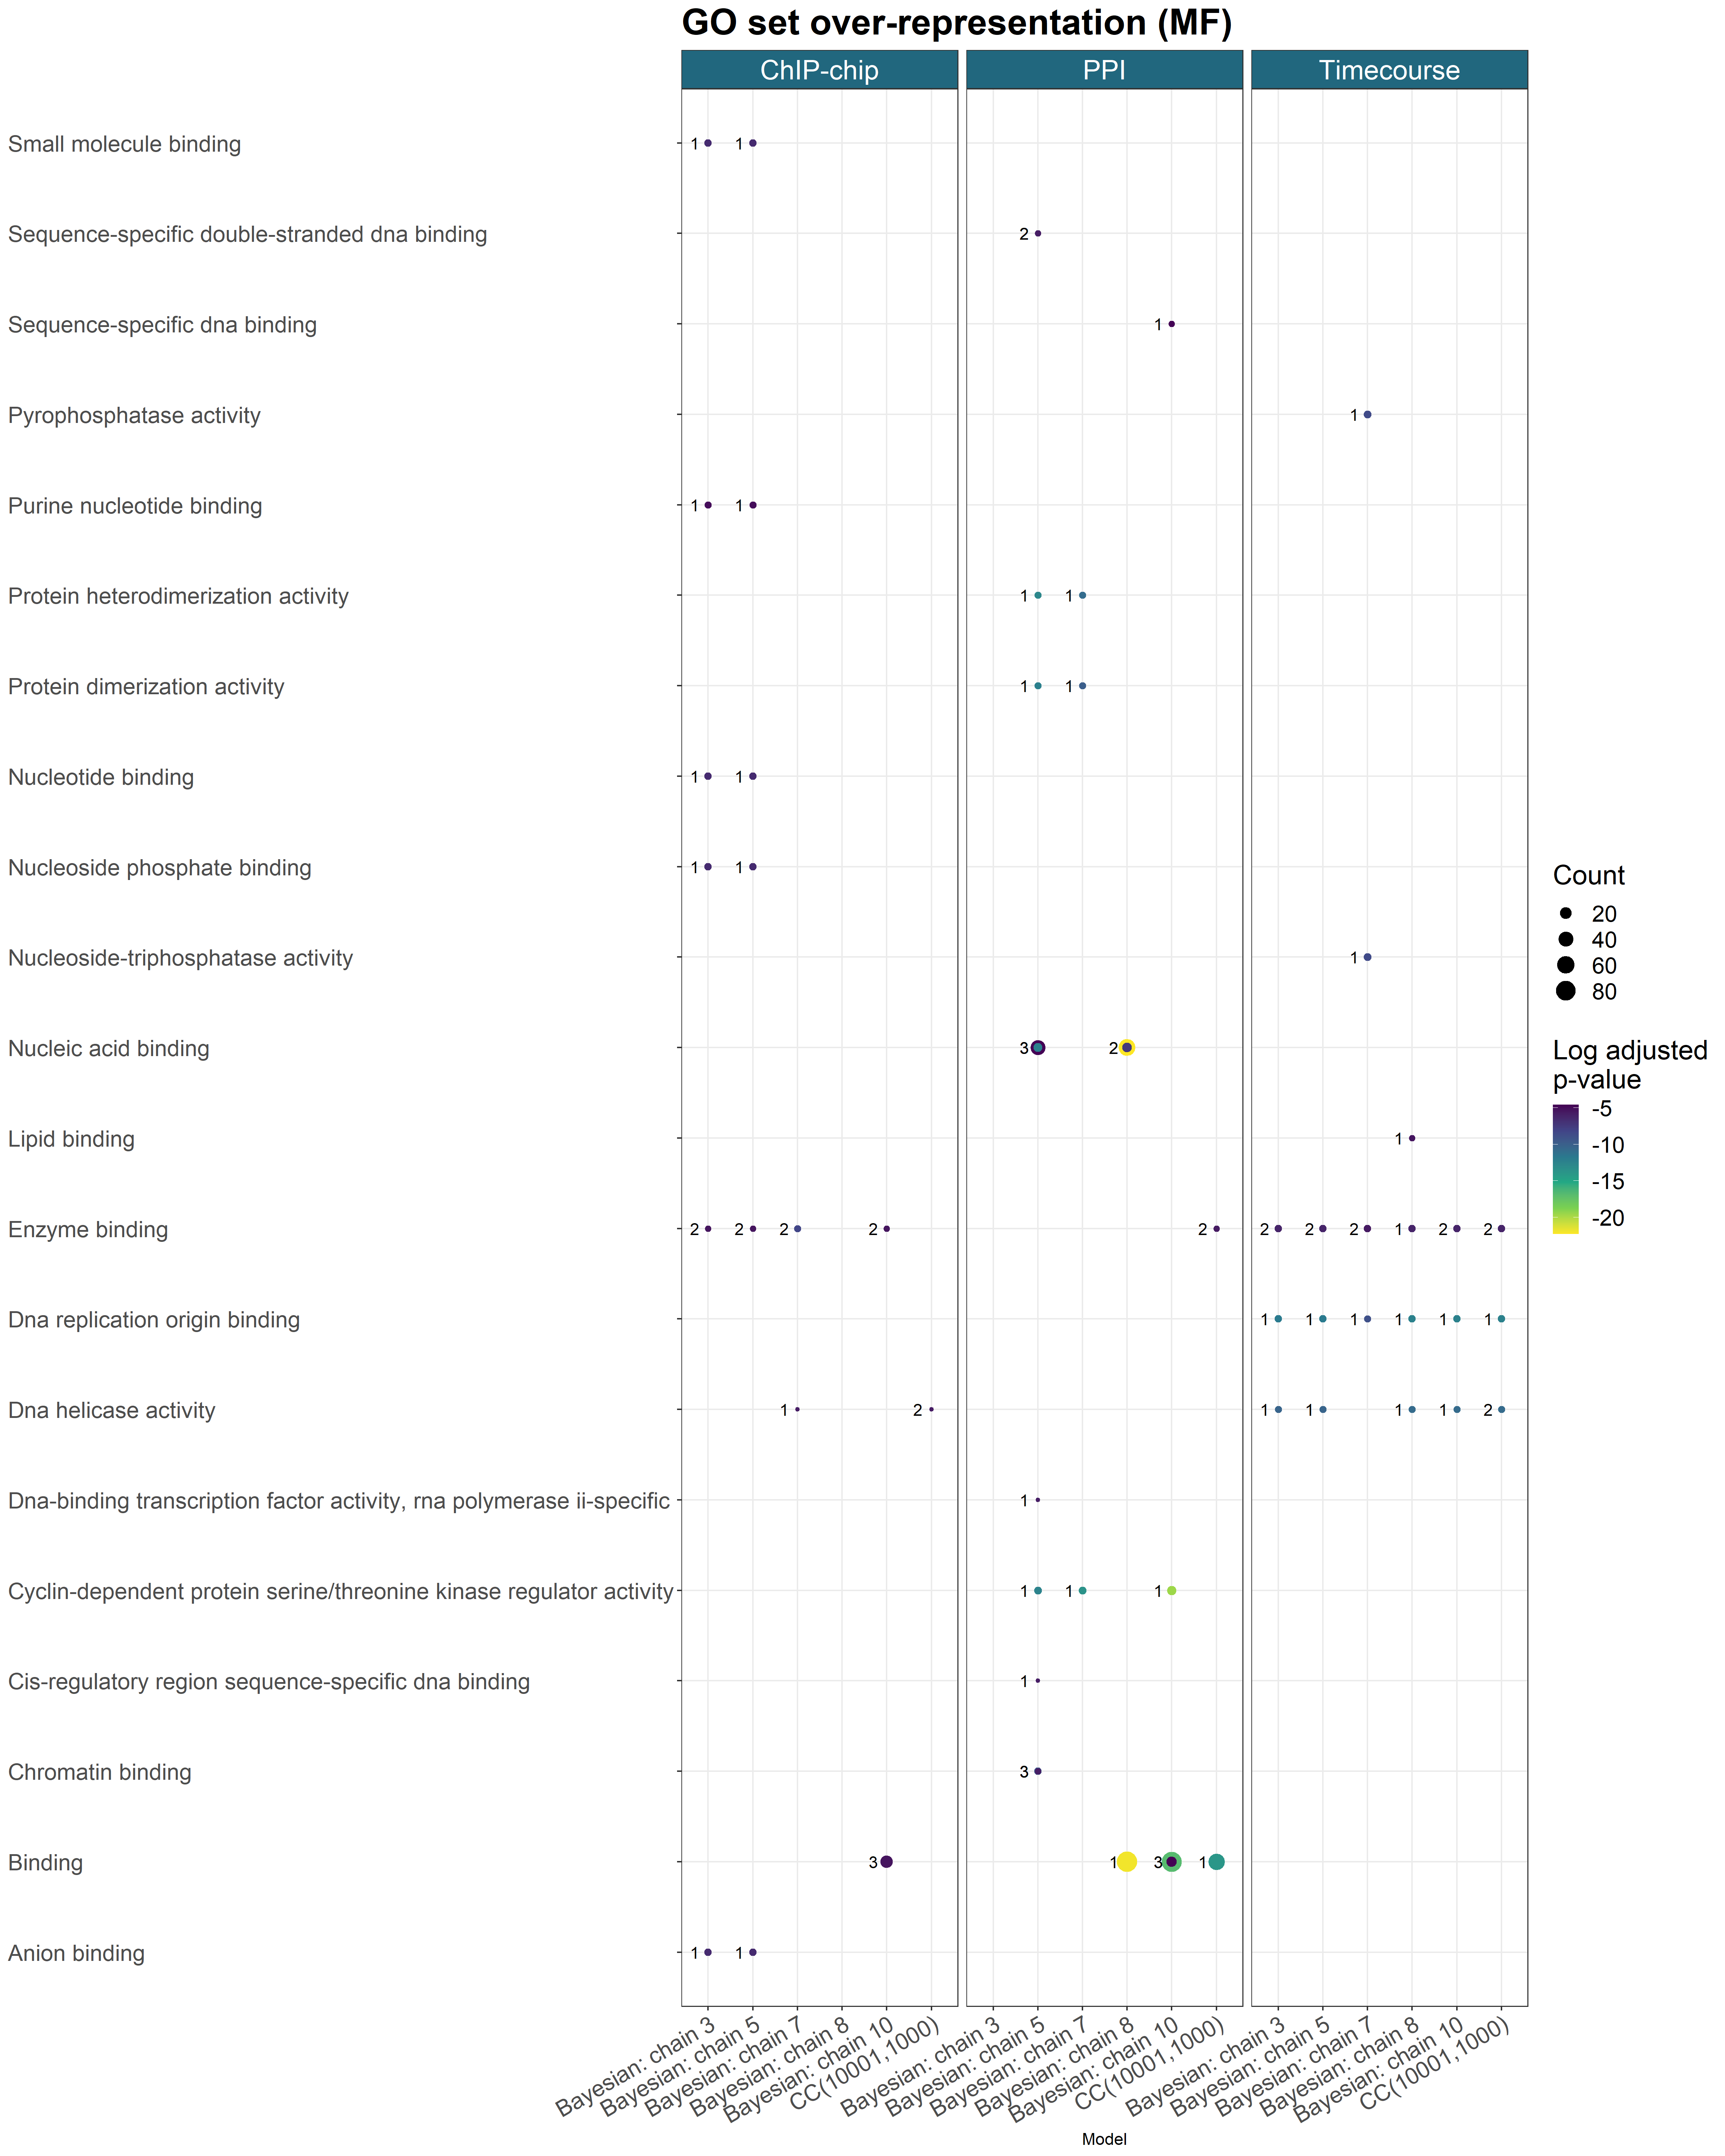
\includegraphics[scale=0.365]{./Images/Yeast/goEnrichmentCompMFvertical.png}
	\caption{GO term over-representation for the Molecular function ontology for each dataset from the final clustering of each method.}
	\label{fig:yeastGOMF}
\end{figure}

\begin{figure}
	\centering
	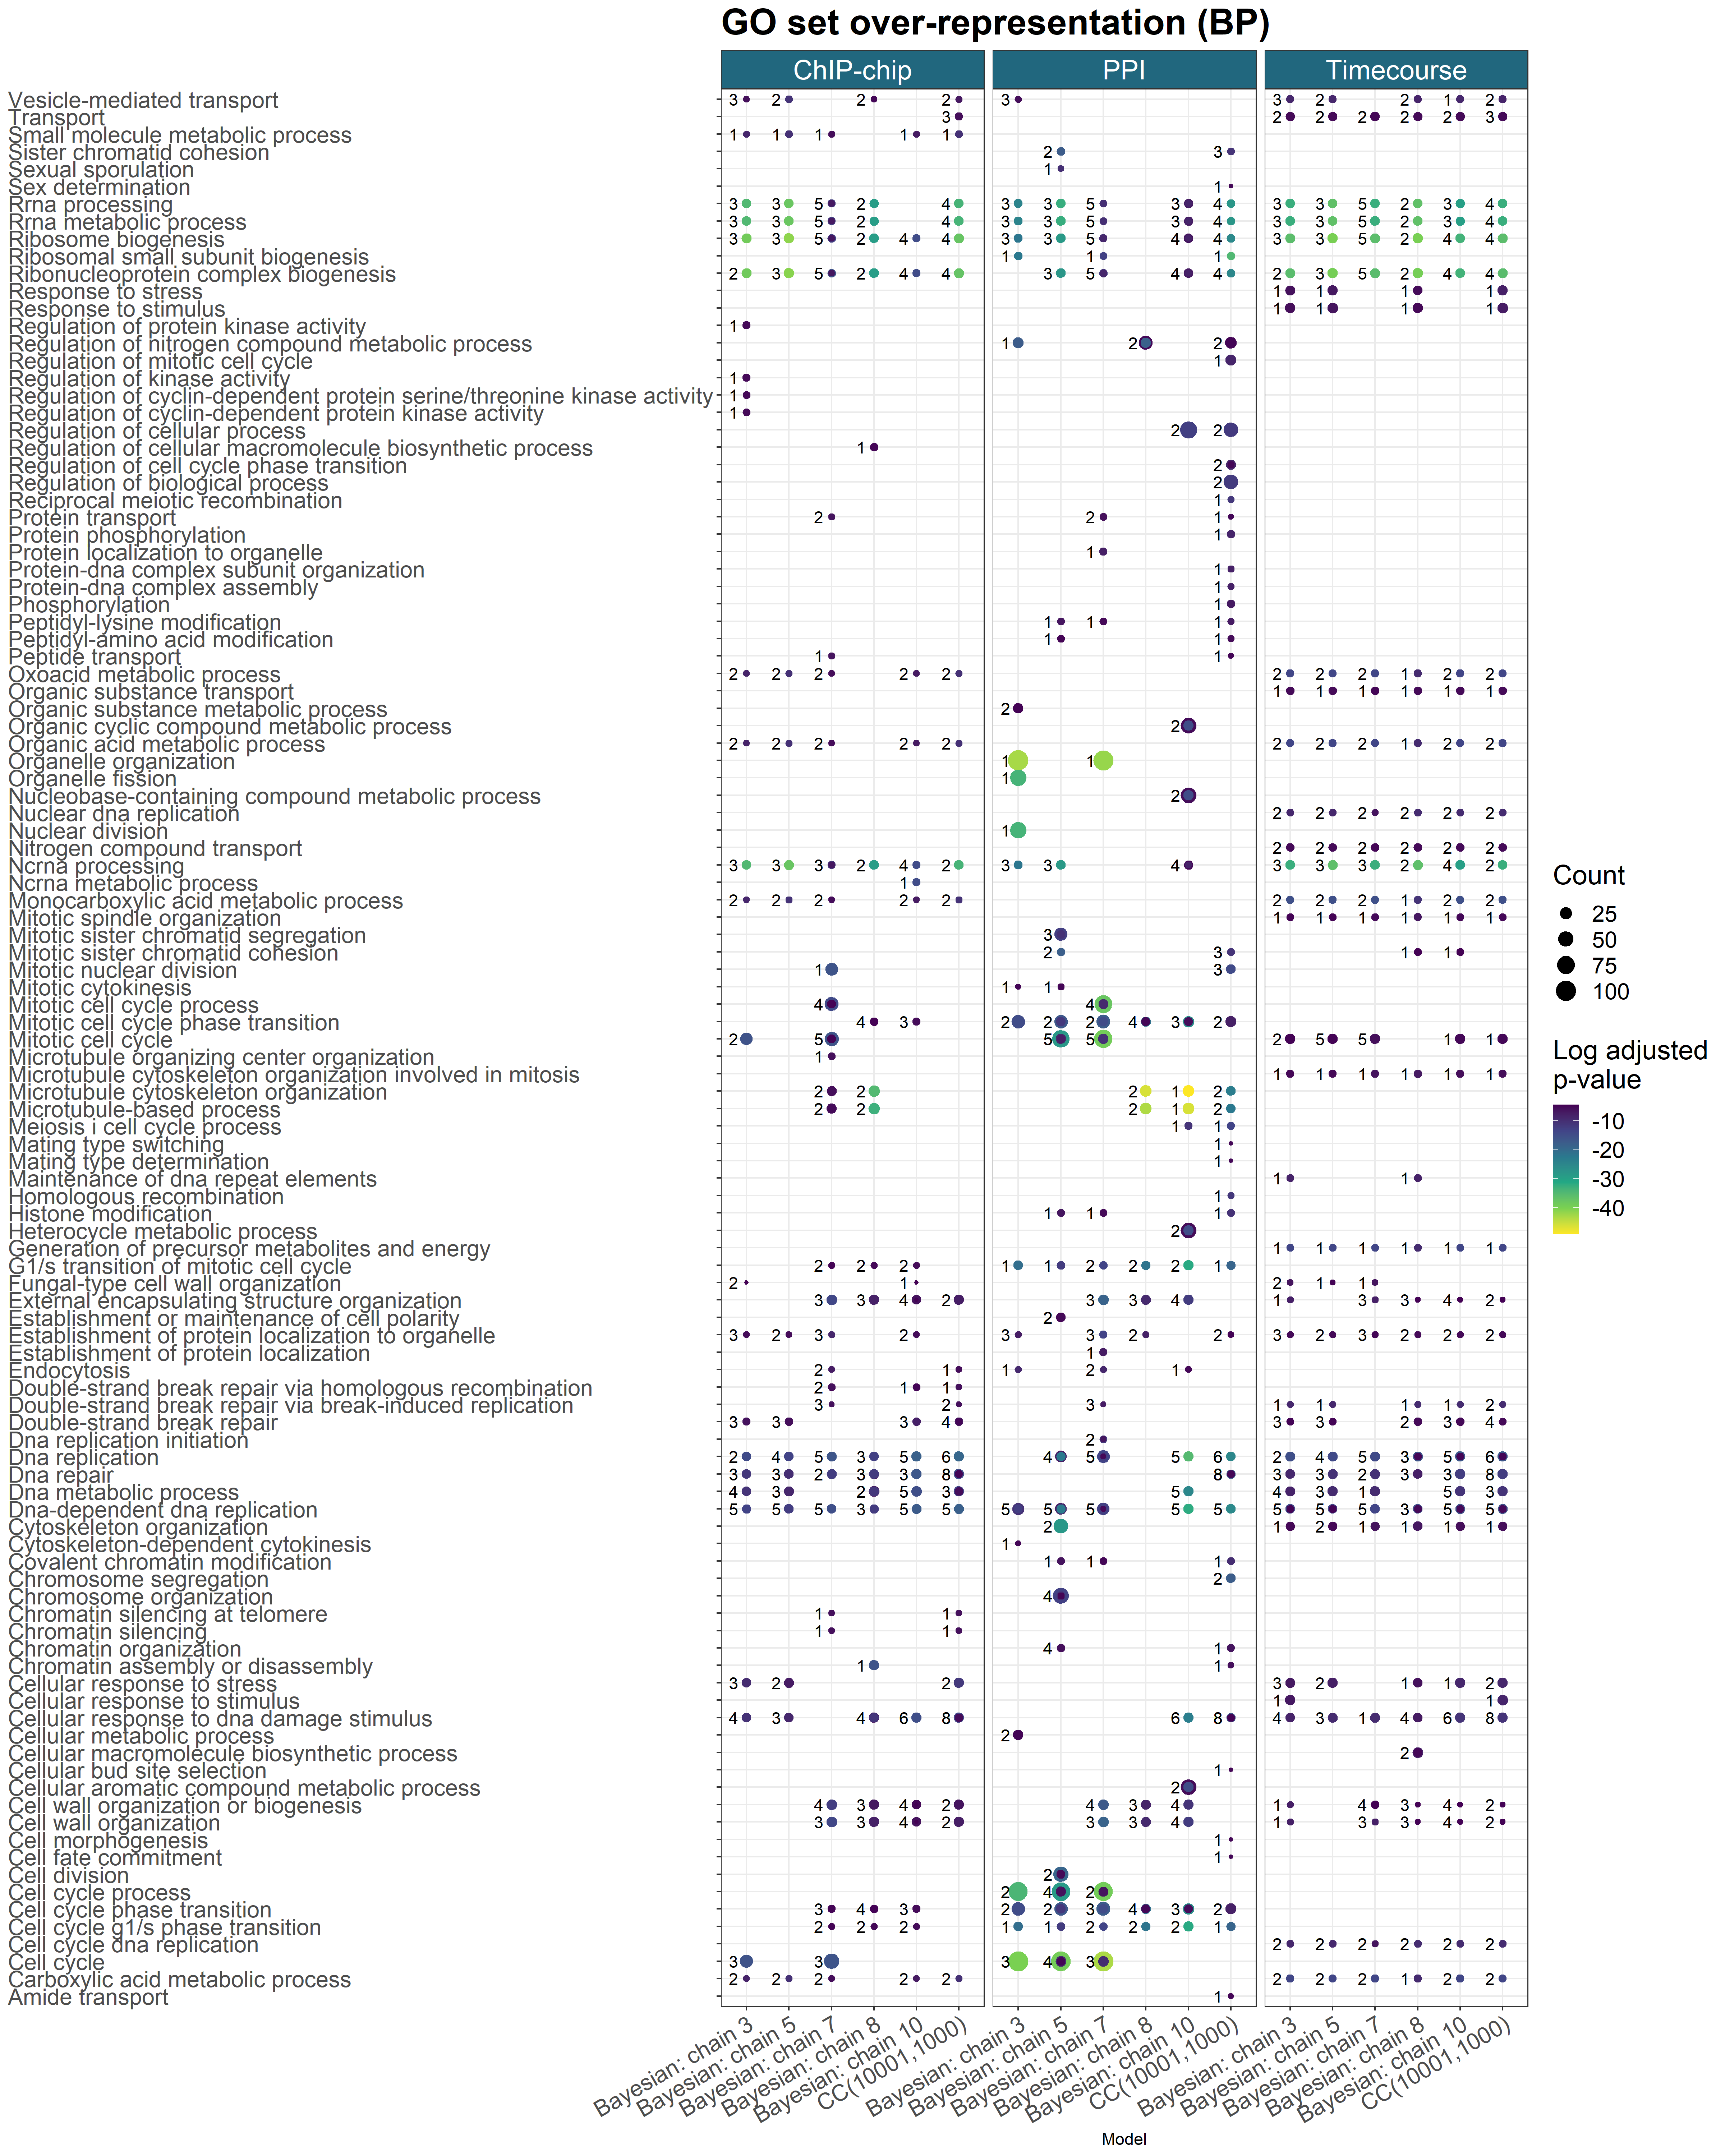
\includegraphics[scale=0.365]{./Images/Yeast/goEnrichmentCompBPvertical.png}
	\caption{GO term over-representation for the Biological process ontology for each dataset from the final clustering of each method.}
	\label{fig:yeastGOBP}
\end{figure}

\begin{figure}
	\centering
	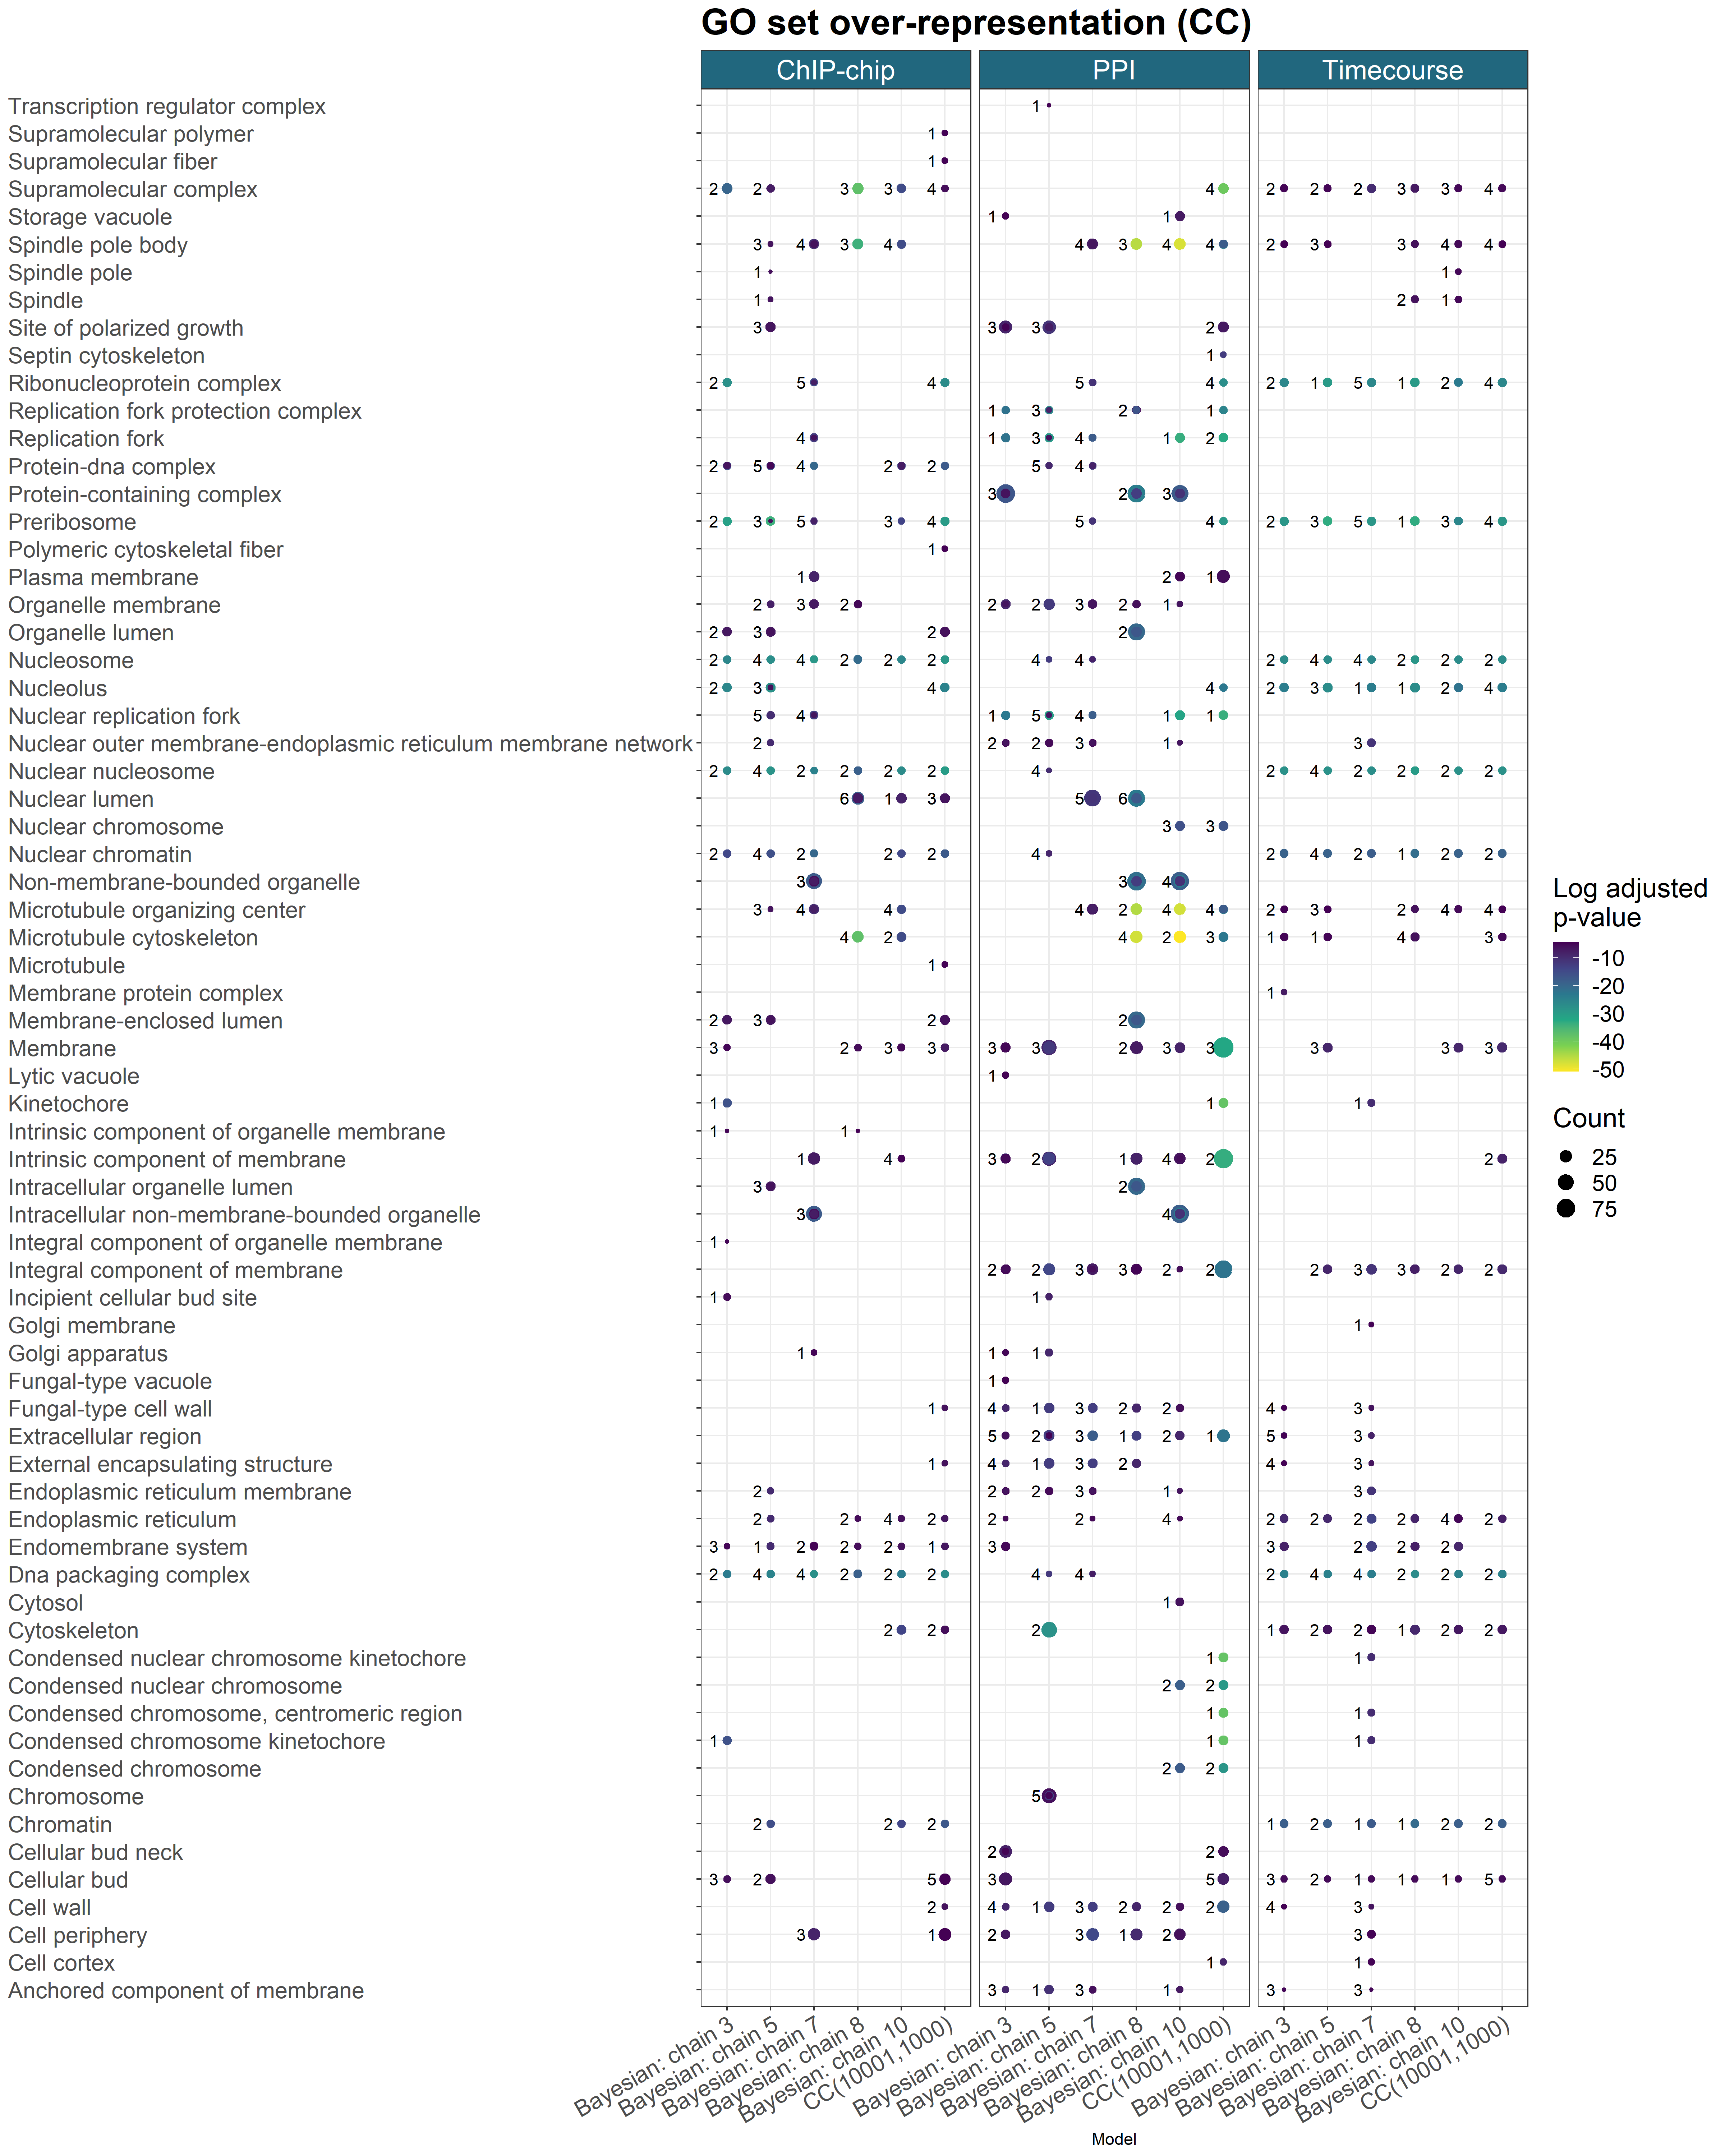
\includegraphics[scale=0.365]{./Images/Yeast/goEnrichmentCompCCvertical.png}
	\caption{GO term over-representation for the Cellular component ontology for each dataset from the final clustering of each method.}
	\label{fig:yeastGOCC}
\end{figure}

%\begin{sidewaysfigure}
%	\centering
%	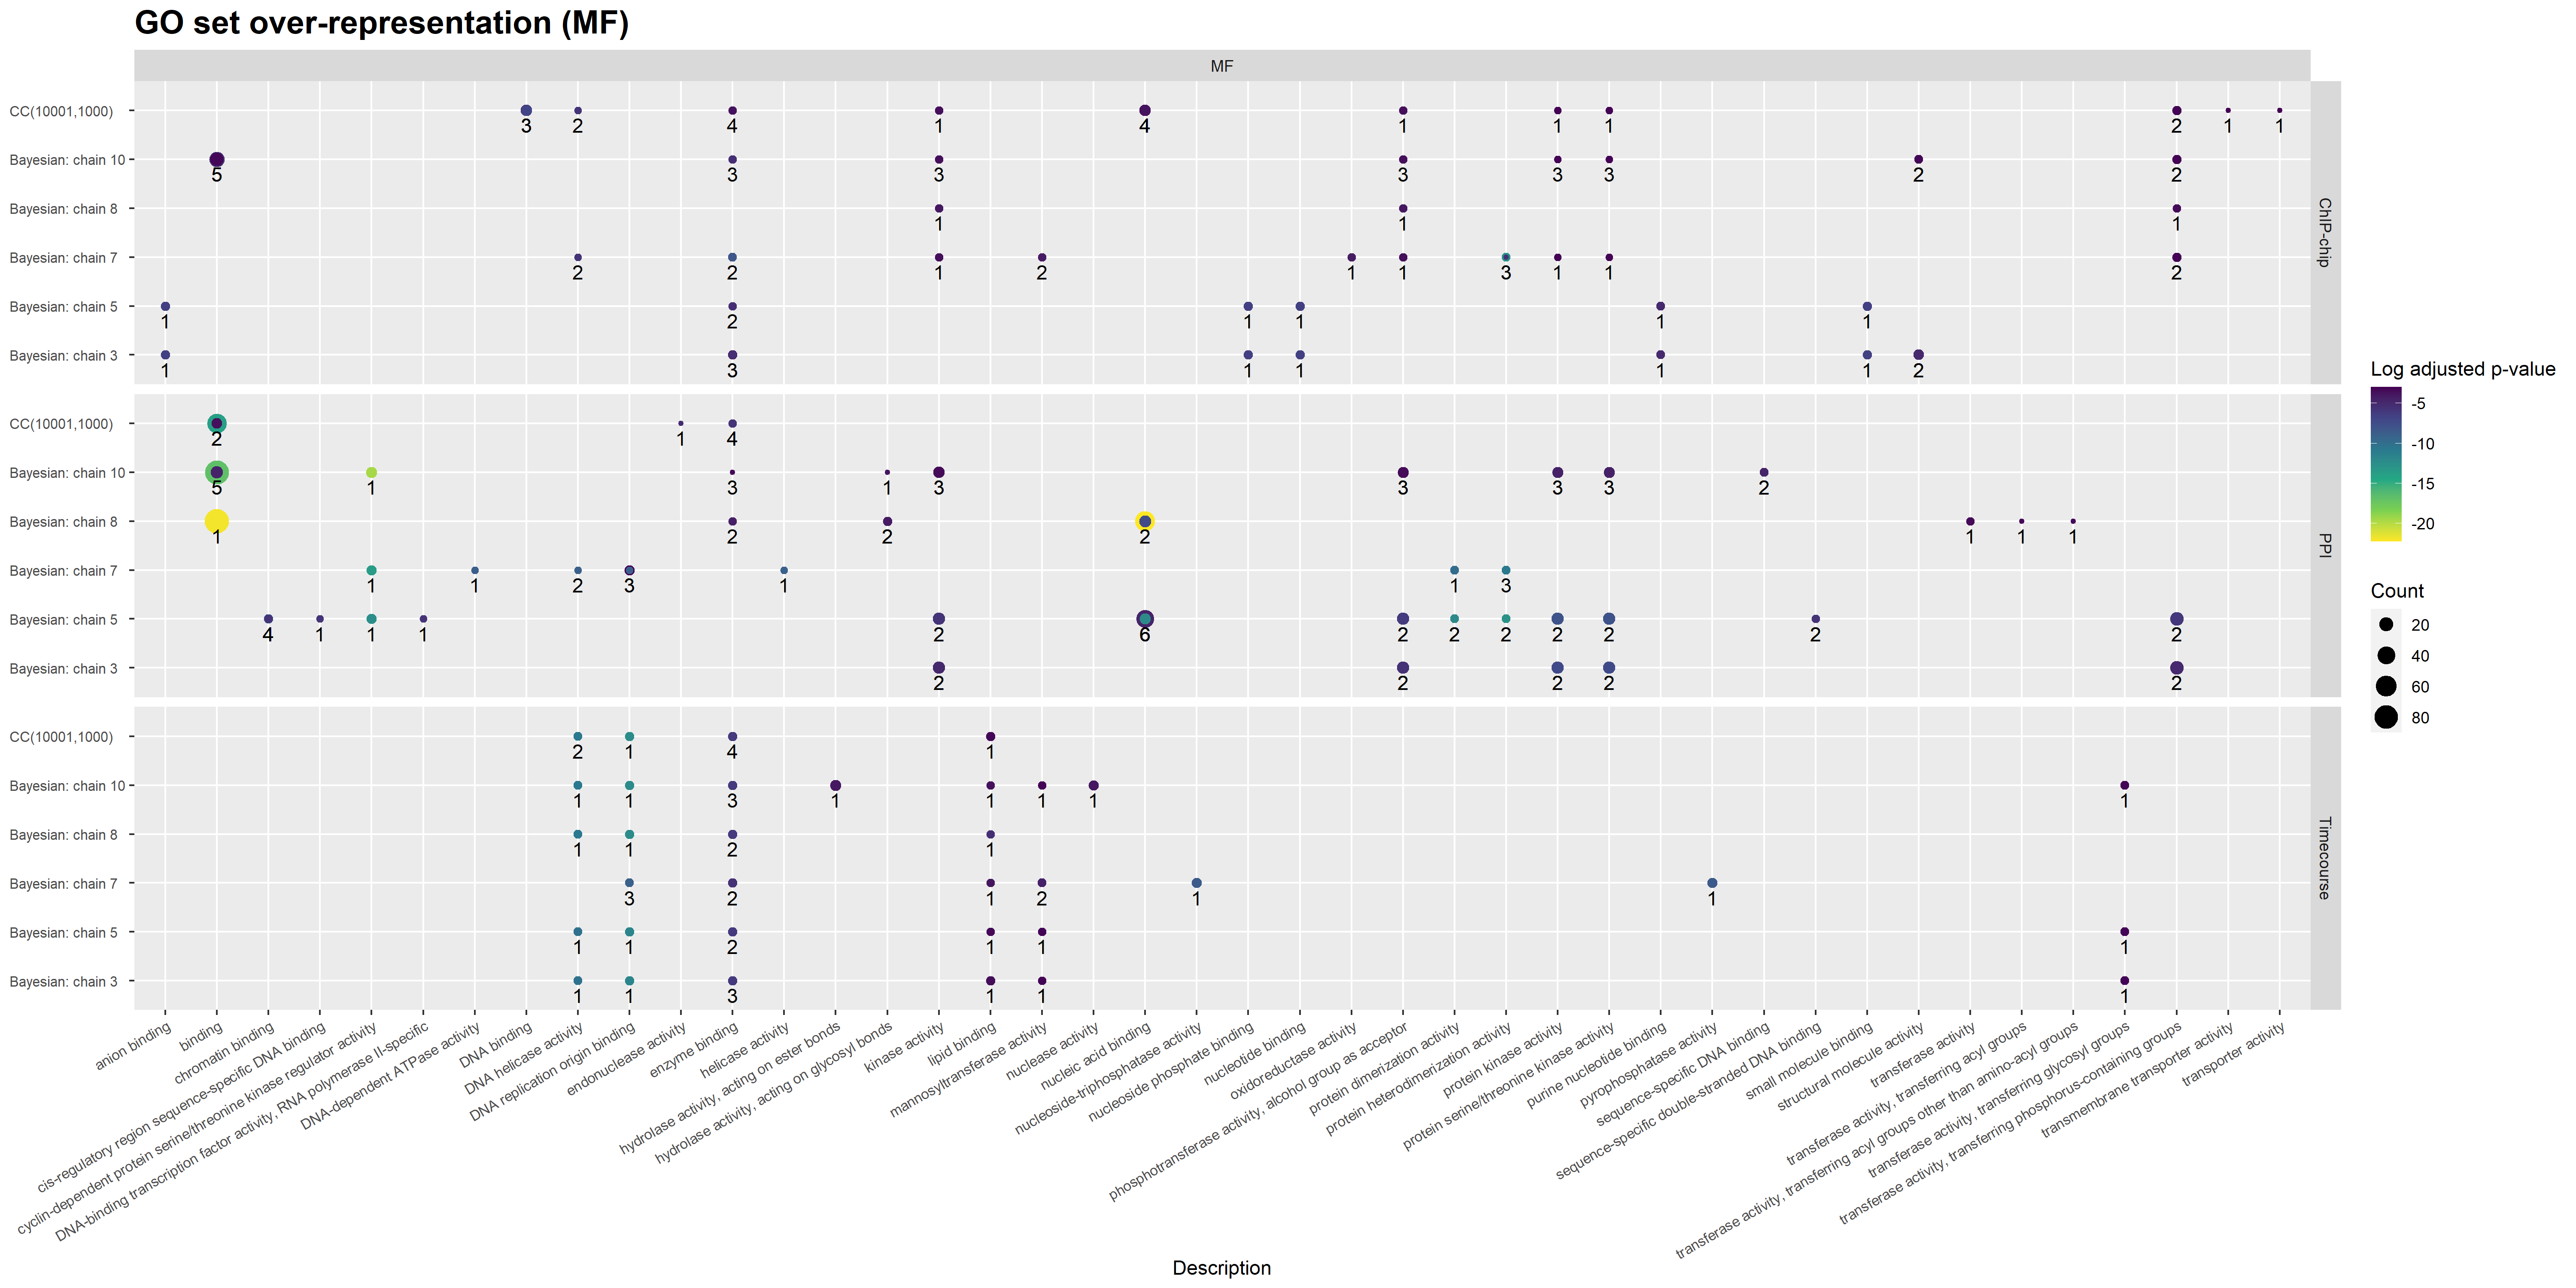
\includegraphics[scale=0.5]{./Images/Yeast/goEnrichmentCompMF.png}
%	\caption{.}
%	\label{fig:yeastGOMF}
%\end{sidewaysfigure}
%
%\begin{sidewaysfigure}
%	\centering
%	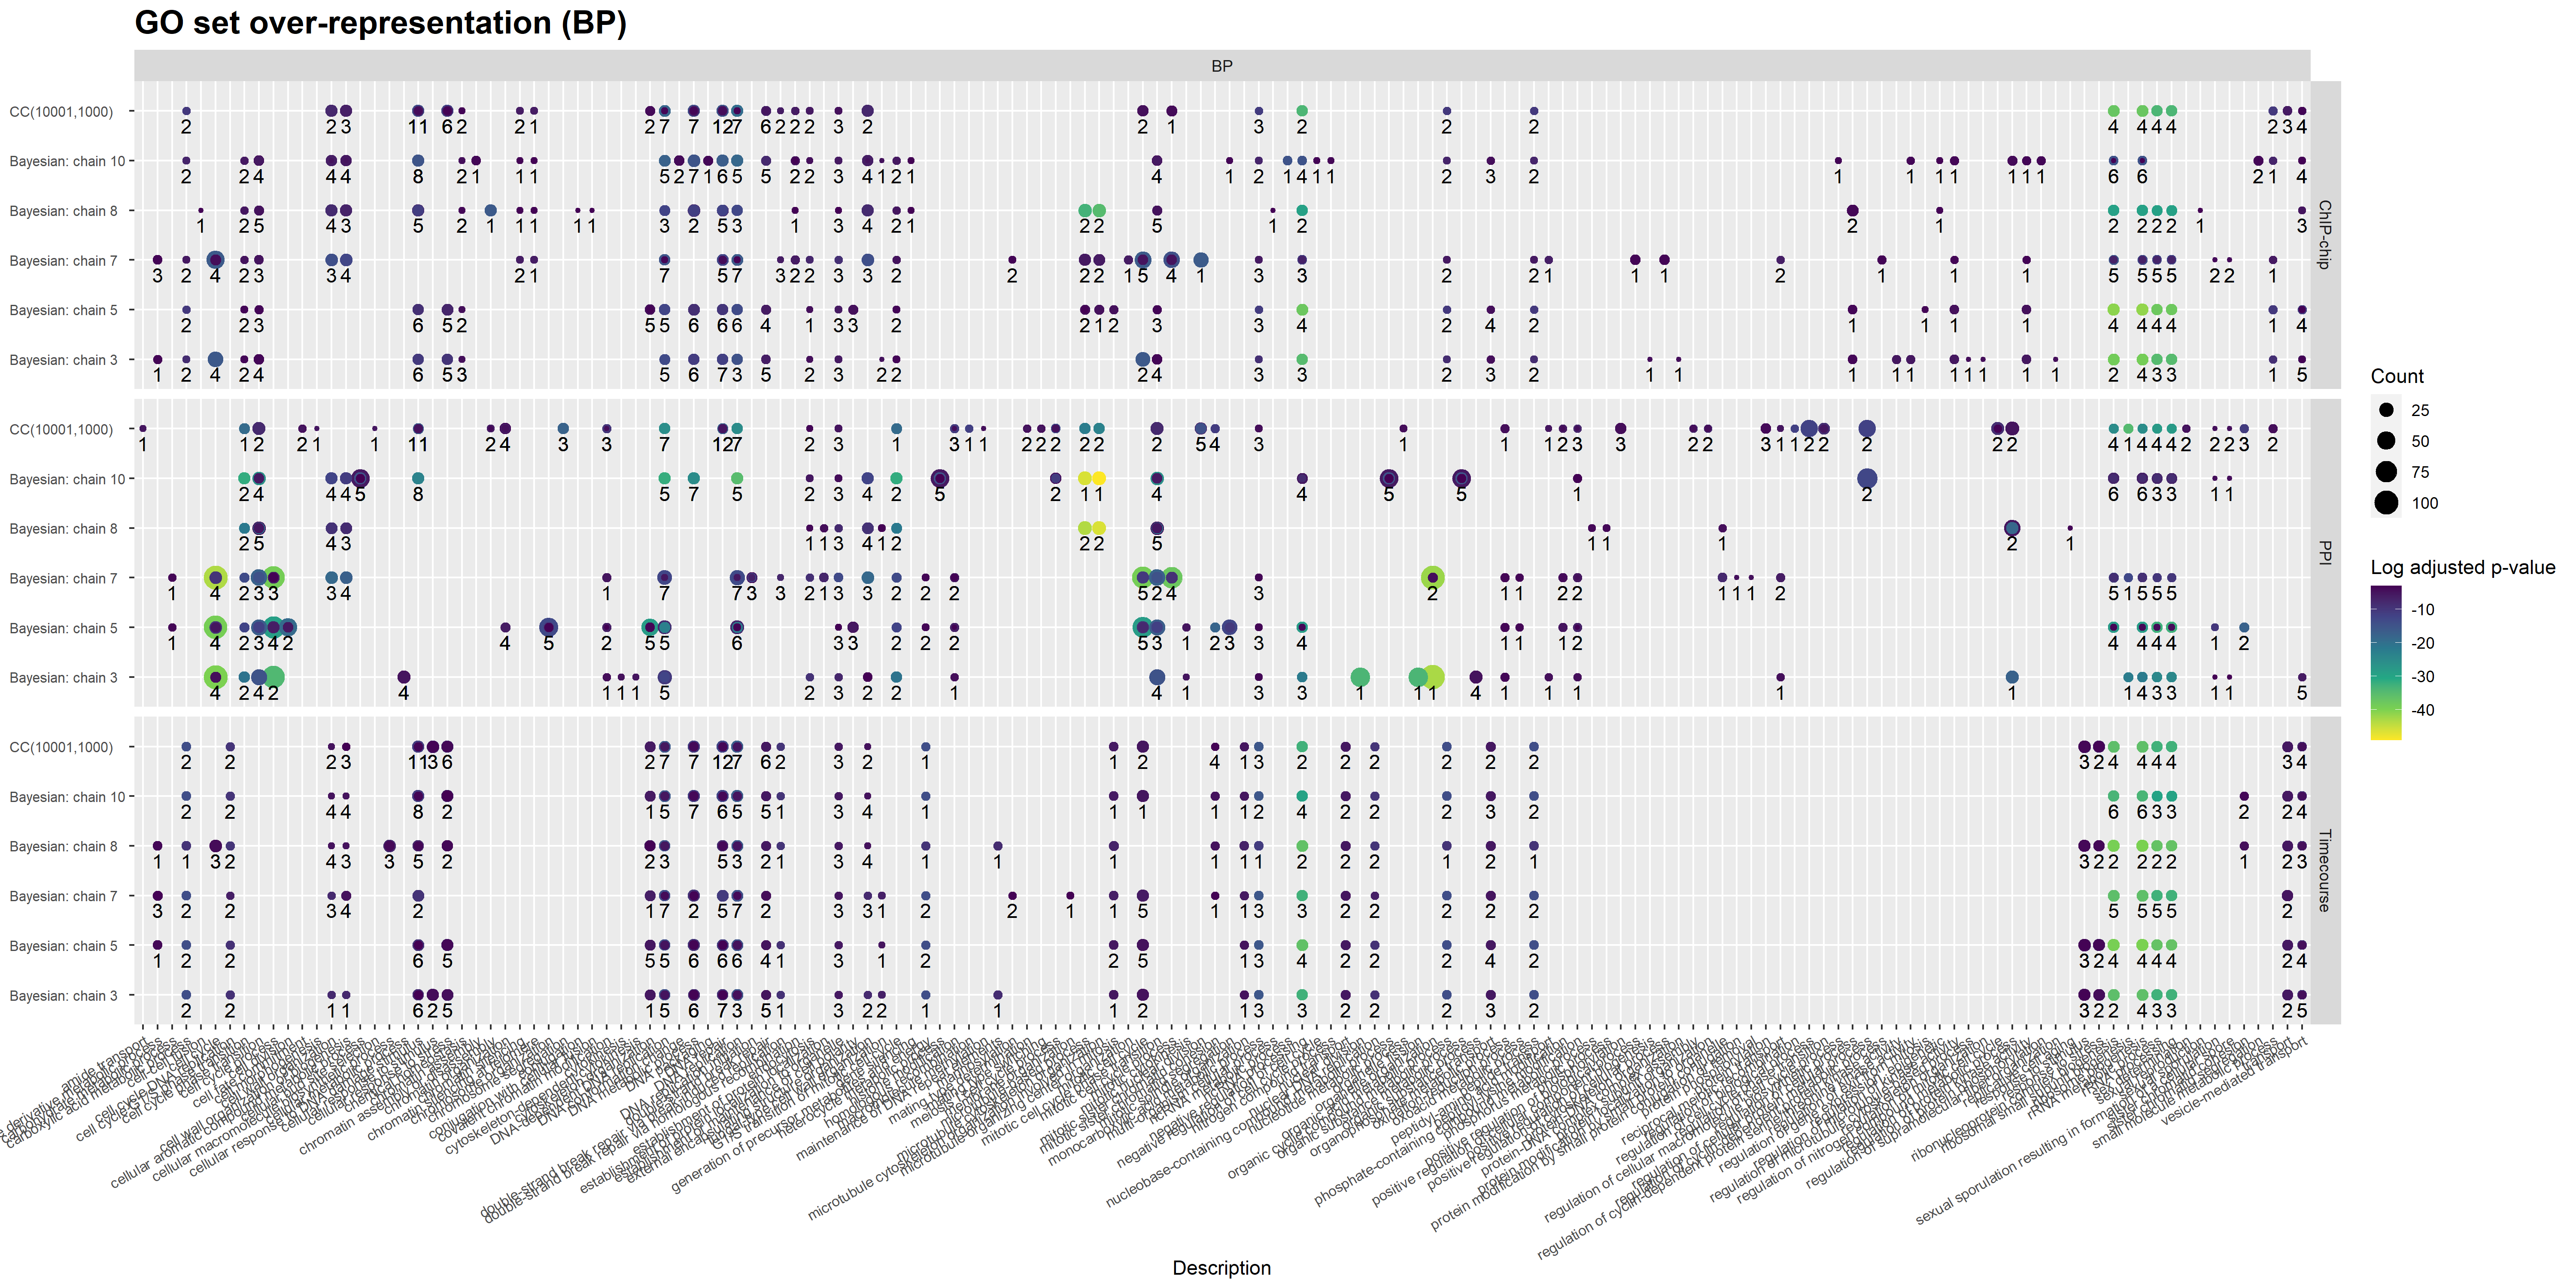
\includegraphics[scale=0.4]{./Images/Yeast/goEnrichmentCompBP.png}
%	\caption{.}
%	\label{fig:yeastGOBP}
%\end{sidewaysfigure}
%
%\begin{sidewaysfigure}
%	\centering
%	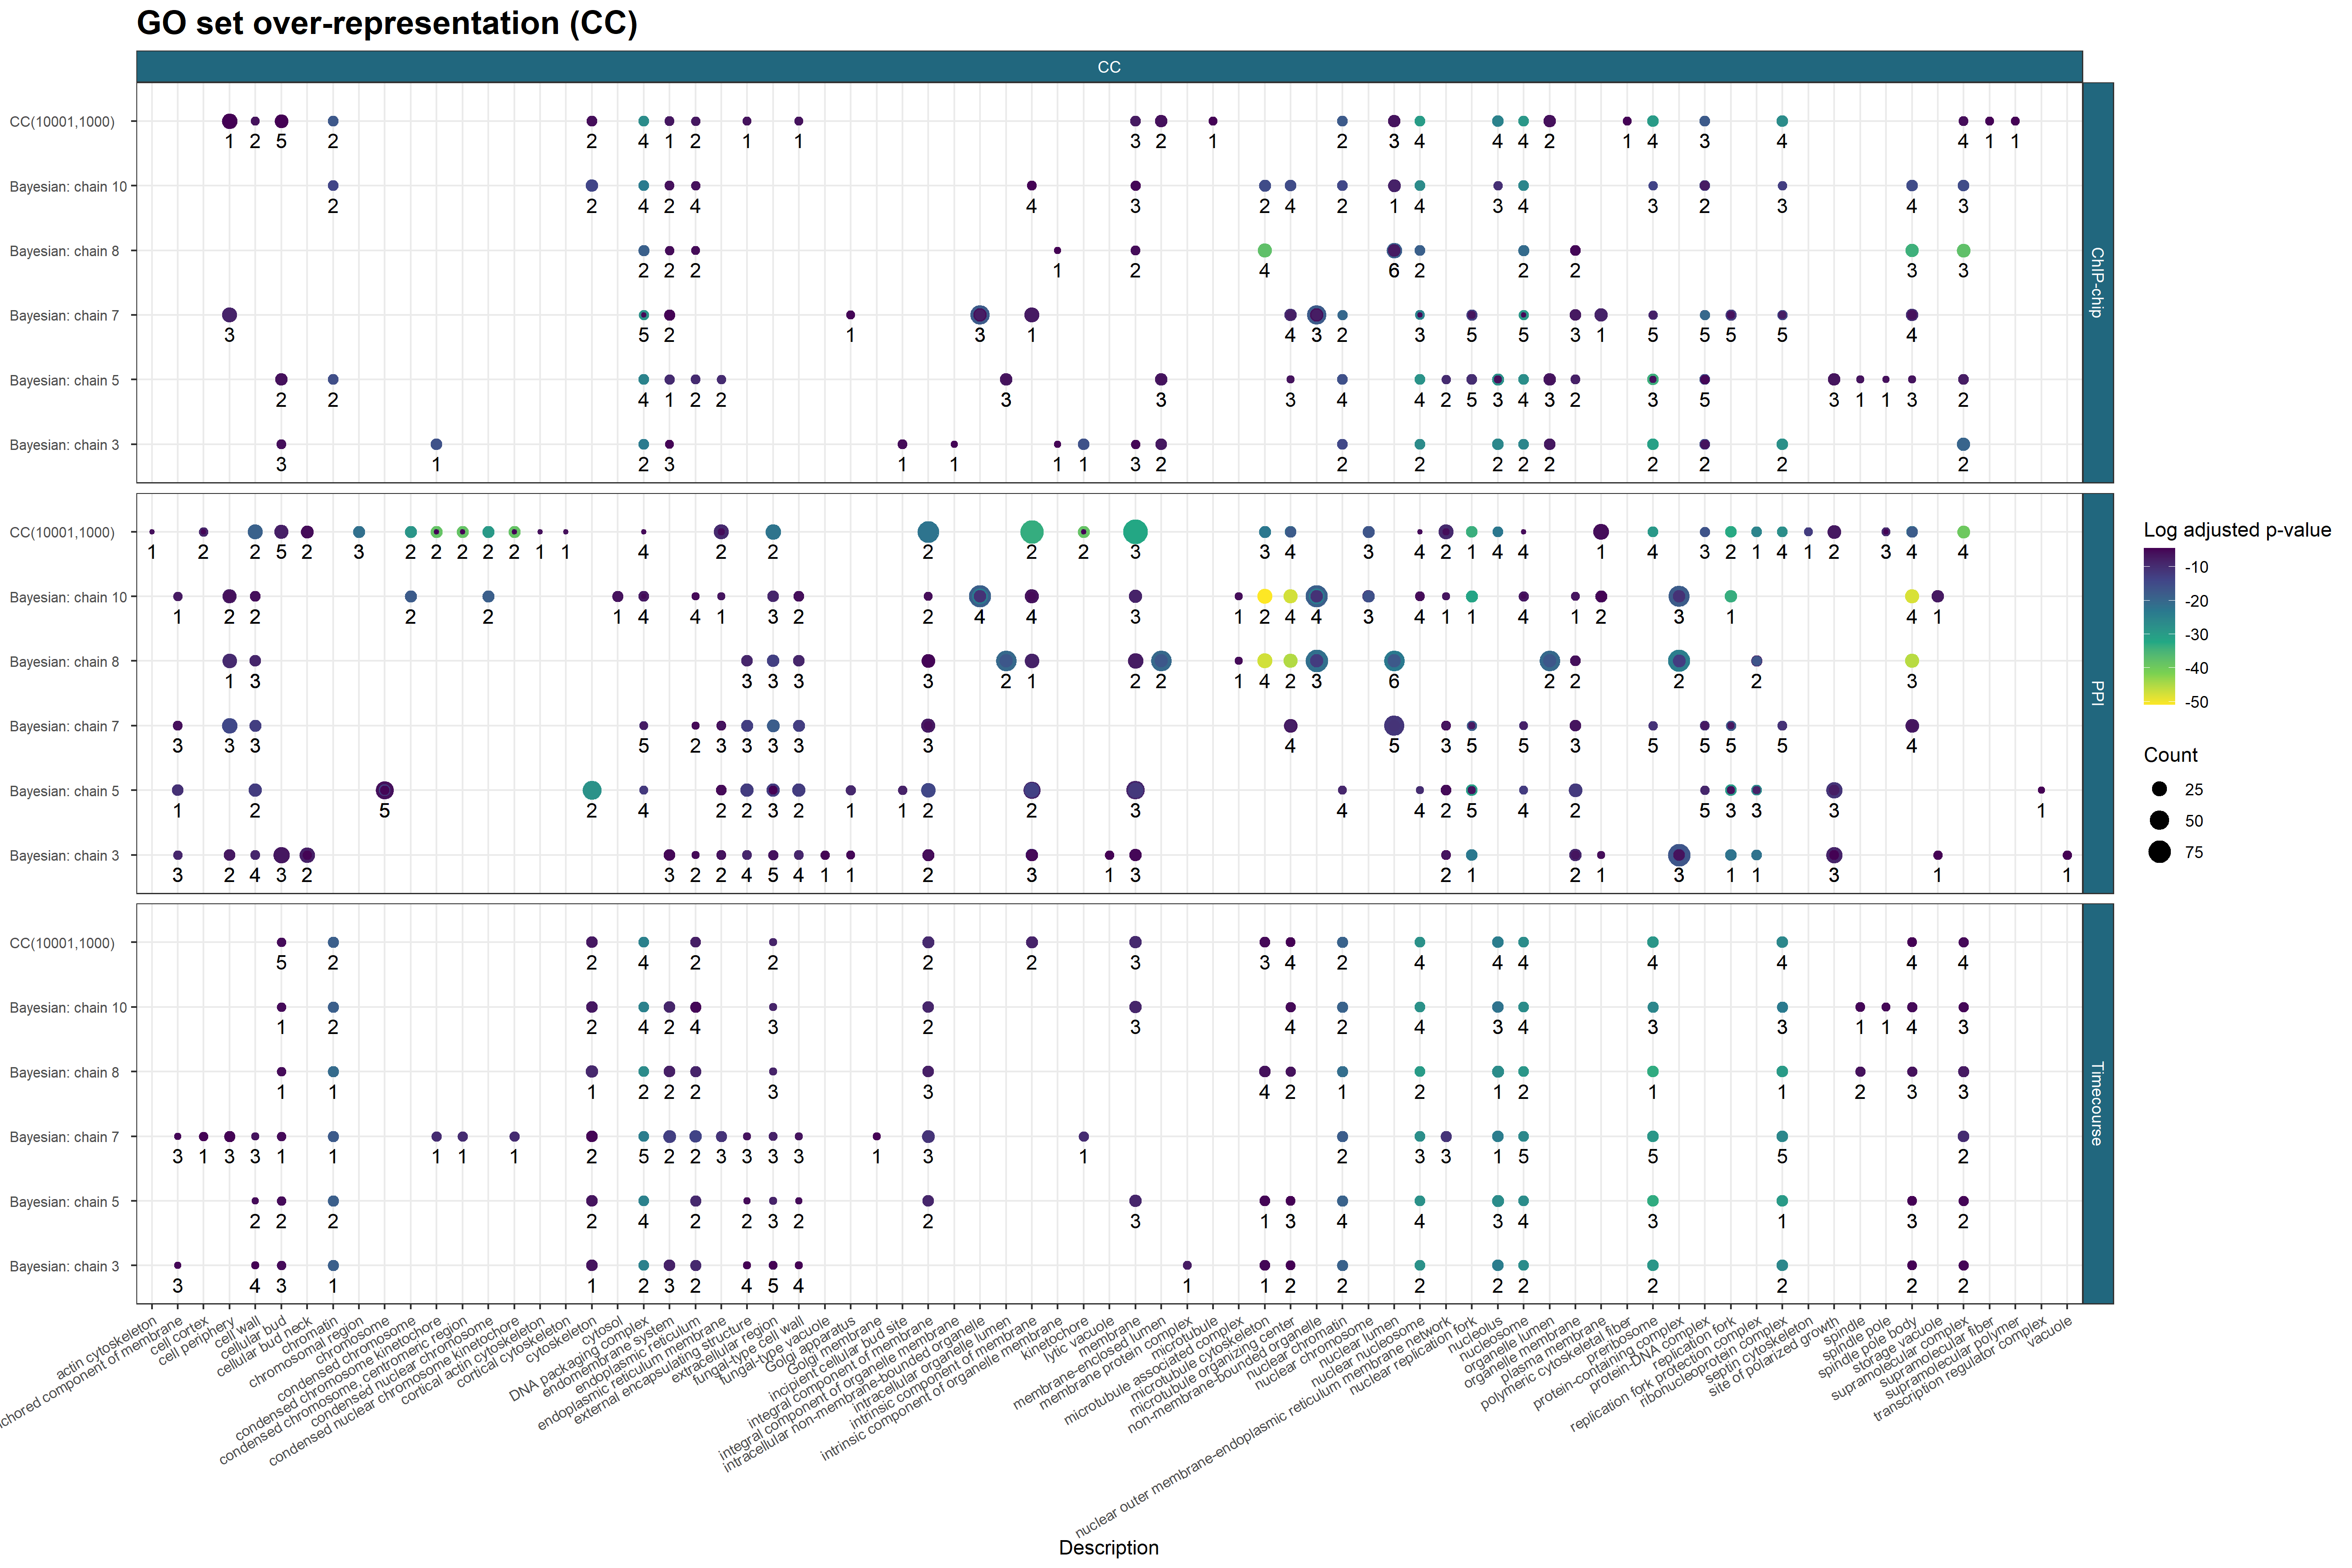
\includegraphics[scale=0.4]{./Images/Yeast/goEnrichmentCompCC.png}
%	\caption{.}
%	\label{fig:yeastGOCC}
%\end{sidewaysfigure}

\bibliographystyle{plainnat}
\bibliography{suppMat}  

\end{document}
